%%%%%%%%%%%%%%%
%%%   TWC %%%%%
%%%%%%%%%%%%%%%

\section{Introduction}

Future generations of cellular networks will provide groundbreaking network capacity, in conjunction with a significantly lower delay and ubiquitous coverage~\cite{Ericss_rep}. \gls{5g} and beyond deployments will support new mobile broadband use cases, e.g., Augmented (AR) and \gls{vr}, and expand into new vertical markets, enabling an unprecedented degree of automation in industrial scenarios, \gls{v2x} communications, remote medical surgery and smart electrical grids.

To this end, the \gls{3gpp} has introduced various technological advancements with the specifications of the \gls{5g} \gls{ran} and \gls{cn}, namely \gls{nr} and \gls{5gc}~\cite{3gpp_38_300}. In particular, \gls{nr} features a user and control plane split, a flexible \gls{ofdm} frame structure, and the support for \gls{mmwave} communications, while the \gls{cn} introduces virtualization and slicing~\cite{yousaf2017nfv}. 

Specifically, the \gls{mmwave} band, i.e., the portion of the spectrum between 30 GHz and 300 GHz, represents the major technological enabler toward the Gbit/s capacity target. These frequencies are characterized by the availability of vast chunks of contiguous and currently unused spectrum, in stark contrast with the crowded sub-6 GHz frequencies. However, \glspl{mmwave} exhibit unfavorable propagation characteristics such as high isotropic losses and a marked susceptibility to blockages and signal attenuation~\cite{khan2011mmwave, rangan2014millimeter}.
These issues can be partially mitigated using beamforming through large antenna arrays, thanks to the small wavelengths and advances in low-power \gls{cmos} RF circuits~\cite{hemadeh2017millimeter}; nevertheless, their introduction alone is not enough for meeting the high service availability requirement. 
Therefore, \glspl{mmwave} networks also need densification, to decrease the average distance between mobile terminals and base stations and improve the average \gls{sinr}. The theoretical effectiveness of this technique is well understood~\cite{gomez2017capacity}; however, achieving dense \gls{5g} deployments is extremely challenging from a practical point of view. Specifically, providing a fiber backhaul among base stations and toward the \gls{cn} is deemed economically impractical, even more so in the initial \gls{5g} deployments~\cite{polese2020integrated}.

Recently, wireless backhaul solutions for \gls{5g} networks have emerged as a viable strategy toward cost effective, dense \gls{mmwave} deployments. Notably, the \gls{3gpp} has promoted \gls{iab}~\cite{3gpp_38_874}, i.e., a wireless backhaul architecture which dynamically splits the overall system bandwidth for backhaul and access purposes. \gls{iab} has been integrated in the latest release of the \gls{3gpp} \gls{nr} specifications. Prior research has highlighted that \gls{iab} represents a cost-performance trade-off~\cite{stoch_geom2, polese2020integrated}, as base stations need to multiplex access and backhaul resources, and as the wireless backhaul at \glspl{mmwave} is less reliable than a fiber connection. In particular, \gls{iab} networks may suffer from excessive buffering (and, consequently, high latency and low throughput) when a suboptimal partition of access and backhaul resources is selected, thus hampering the benefits that the high bandwidth \gls{mmwave} links introduce~\cite{polese2020integrated,polese2018end}. Therefore, it is fundamental to solve these non-trivial challenges to enable a smooth integration of \gls{iab} in \gls{5g} and beyond deployments.
%TODO need for optimization of the resource allocation ?

\subsection{Contributions}
\label{sec:contributions}

This article tackles the access and backhaul partitioning problem by proposing an optimal, semi-centralized resource allocation scheme for \gls{3gpp} \gls{iab} networks, based on the \gls{mwm} problem on graphs.  It receives periodic L1 and/or L3 measurements from the nodes of the \gls{iab} deployment, a possibility which is explicitly mentioned by 3GPP in~\cite[Sec. 7.3.3]{3gpp_38_874}, constructs a spanning tree that represents the deployment, and uses a simplified, low-complexity version of the \gls{mwm} to partition the links between access and backhaul. After a feedback step, each node can then schedule the resources at a subframe-level among the connected devices. 

To the best of our knowledge, this is the first \gls{mwm}-based resource allocation framework for \gls{3gpp} \gls{iab} networks at \glspl{mmwave}. As such, it exhibits the following benefits:
\begin{enumerate*}[label=(\roman*)]
  \item no constraints on the number of hops in the \gls{iab}-network are introduced, and, more in general, it is \gls{3gpp}-compliant;
  \item a globally optimum is computed;
  \item generic network utility functions can be used;
  \item it features a computational complexity which is linear in the number of \glspl{gnb} which are connected to the same \gls{iab}-donor; and 
  \item a very limited communication overhead is required.
\end{enumerate*}

In particular, the flexibility makes it possible to easily adapt the resource allocation strategy to different requirements, use cases, and classes of traffic for \gls{5g} networks. We achieve this by developing a generic optimization algorithm, which identifies with a configurable periodicity the access and backhaul partition that optimizes a certain utility function. The selection of the utility function prioritizes the optimization of different metrics, e.g., throughput or latency, which in turn can be mapped to different classes of traffic.

Moreover, to achieve the compliance with the \gls{3gpp} \gls{iab} specifications, the resource allocation framework relies only on information that can be actually exchanged and reported in a \gls{3gpp} deployment. In this regard, we also review the latest updates related to the \gls{3gpp} \gls{iab} standardization activities. Nevertheless, our solution can be easily extended to consider other types of feedback information.
Finally, the algorithm operates with a low complexity, i.e., we propose a version of the \gls{mwm} algorithm that can be applied on spanning trees with linear complexity in the number of nodes in the network infrastructure, and demonstrate its equivalence to the generic (and more complex) \gls{mwm}. Additionally, the proposed framework also relies on a feedback exchange that is linear in the number of base stations, and is thus decoupled from the number of users. Along this line, the semi-centralized nature of the proposed solution combines the benefit of a centralized point of view for the allocation of inter-dependent \gls{iab} links and a limited complexity.

Furthermore, we evaluate the performance of the proposed scheme with an end-to-end, full-stack system-level simulation, using the ns-3 mmWave module~\cite{mezzavilla2018end} and its \gls{iab} extension~\cite{polese2018end}. This represents the first evaluation of an optimized resource allocation scheme for \gls{iab} with a simulator that is based on a \gls{3gpp}-compliant protocol stack, uses \gls{3gpp} channel models, and integrates realistic applications and transport protocols. The extended performance evaluation highlights how the proposed scheme improves the throughput of a diverse set of applications, with a 5-fold increase for the worst case users, with different packet sizes and transport protocols, while decreasing the latency and buffering at intermediate nodes by up to 25 times for the smallest packet sizes.

\subsection{State of the Art}
%TODO keep this subdvision wrt to the approach ? 
%TODO slim down
% Since this new-found interest on wireless backhauling for cellular networks is relatively recent, such topic has not been exhaustively studied yet. Nevertheless, m

% Multi-hop wireless networks have been already thoroughly studied in scenarios others from cellular networks, for instance in the context of wireless mesh networks~\cite{gambiroza2004end}. 
This section reviews relevant research on resources allocation in a multi-hop wireless network, deployed through either \gls{iab} or other wireless mesh solutions~\cite{gambiroza2004end}.

The literature adopts different approaches to model and solve the resource allocation problem. The first, discussed in~\cite{qualcomm1, qualcomm2, kulkarni2018max, lei2020deep, rasekh2015interference, bilal2014time, cruz2003optimal} is based on conventional optimization techniques.
Specifically, the authors of~\cite{qualcomm1} present a simple and thus tractable system model and find the minimal number of \glspl{gnb} featuring a wired backhaul that are needed to sustain a given traffic load. Their work is further extended in~\cite{qualcomm2}, which provides an analysis of the performance benefits introduced by additional, fiber-less \glspl{gnb}. 
In~\cite{kulkarni2018max}, the mobile network is modeled as a noise-limited, $k$-ring deployment. Such model is then used to obtain closed-form expressions for the max-min rates achieved by \glspl{ue} in the network. Moreover,~\cite{lei2020deep} proposes a system model which leads to an NP-hard optimization problem, even though it considers single-hop backhaul networks only, and uses deep \gls{rl} to reduce its computation complexity. In~\cite{rasekh2015interference}, the joint routing and resource allocation problem is tackled via a \gls{lp} technique. Notably, this work assumes that data can be transmitted (received) toward (from) multiple nodes at the same time.
Similarly, the authors of~\cite{bilal2014time} formulate a \gls{tdd}, multi-hop resource allocation optimization problem which leverages the directionality of \gls{mmwave} antennas, albeit in the context of \gls{wpans}. Since such problem is also NP-hard, a sub-optimum solution is found. Finally,~\cite{cruz2003optimal} focuses on joint link scheduling, routing and power allocation in multi-hop wireless networks. As in previous cases the obtained optimization problem is not tractable: in this instance such obstacle is overcome by studying the dual problem via an iterative approach.

%On the contrary, a portion of the available literature such as~\cite{semiari2015matching, loumiotis2014dynamic} tackles the resource allocation problem by using game theory. In particular, the authors of~\cite{semiari2015matching} formulate the optimization problem as a one-to-many matching game, obtaining a distributed algorithm that manages to outperform a best-effort approach; however, such analysis is limited to single-hop wireless networks. In~\cite{loumiotis2014dynamic}, the system is modeled as a multi-operator network where the former receive an utility that takes into account their backhaul usage cost. As a consequence, the game-theory-based algorithm that the authors propose aims at achieving an asymptotically stable allocation by targeting an equilibrium between the subscriber fees (hence, the amount of backhaul resources needed) and the fulfillment of the user requirements.

The second approach relies on stochastic geometry to model \gls{iab} networks~\cite{stoch_geom1, stoch_geom2}. Specifically,~\cite{stoch_geom1} determines the rate coverage probability of \gls{iab} networks and compares different access/backhaul resource partitioning strategies. Similarly,~\cite{stoch_geom2} provides a comparison of orthogonal and integrated resource allocation policies, although limited to single-hop wireless networks.  

Another significant body of literature leverages \glspl{mc} to study \gls{iab} networks; some of these works can be interpreted as a direct application of such theory~\cite{singh2018throughput, ji2012throughput}, while others~\cite{vu2018path,garcia2015analysis, gomez2016optimal, gomez2019optimal} exploit a more complex framework.  
The papers which belong to the former class are based on the  pioneering work of~\cite{tassiulas1990stability}, which inspects the stability of generic multi-hop wireless networks and formulates a throughput-maximizing algorithm known as \textit{back-pressure}. In particular,~\cite{singh2018throughput} focuses on the optimization of the timely-throughput, i.e., takes into account that packets usually have an arrival deadline. Such problem is then addressed by formulating a \gls{mdp}, leading to a distributed resource allocation algorithm. Similarly,~\cite{ji2012throughput} proposes an algorithm that also targets throughput optimality but, contrary to the back-pressure algorithm, manages to avoid the need for per-flow information.
On the other hand, the body of literature which belongs to the latter class uses the \gls{mc}-derived \gls{num} framework first introduced in~\cite{kelly1997charging} and ~\cite{kelly1998rate}. Specifically, the authors of~\cite{vu2018path} focus on satisfying the \gls{urllc} \gls{qos} requirements by jointly optimizing routing and resource allocation. Then, 
%the problem is decoupled into two successive phases, the first exploiting \gls{rl} for achieving an optimal routing and the latter employing convex optimization in order to solve the resource allocation problem%
the problem is solved using both convex optimization and \gls{rl} techniques. In~\cite{garcia2015analysis}, an in-depth analysis of a \gls{mmwave}, multi-hop wireless system is presented, proposing and comparing three different interference frameworks, under the assumption of a dynamic \gls{tdd} system. This work is extended in~\cite{gomez2016optimal} and~\cite{gomez2019optimal}, which consider respectively a \gls{sdma} and a \gls{mu}-\gls{mimo} capable system.

Finally, only a small portion of the literature~\cite{polese2018end, polese2018iab, polese2020integrated} analyzes the end-to-end performance of \gls{iab} networks. Specifically, the authors of~\cite{polese2018end} extend the ns-3 \gls{mmwave} module, introducing realistic \gls{iab} functionalities which are then used to characterize the benefit of deploying wireless relays in \gls{mmwave} networks. Their work is extended in~\cite{polese2018iab}, where path selection policies are formulated and their impact on the system performance is inspected. A further end-to-end analysis of \gls{iab} networks is carried out in~\cite{polese2020integrated}, providing insights into the potentials of this technology and the related open research challenges.

Concluding, the literature exhibits the presence of algorithms relying on a varying degree of assumptions on the network topology and the knowledge of system. Furthermore, most of the aforementioned studies lack an end-to-end, full-stack system-level analysis of the proposed solution.
Conversely, this paper proposes a semi-centralized resource allocation scheme, which also has a low complexity, both computationally and in terms of required feedback. Moreover, we provide considerations on how our proposed solution can be implemented and deployed in standard-compliant \gls{3gpp} \gls{iab} networks, and compare such solution to the state of the art with an end-to-end, realistic performance analysis.

\subsection{Paper structure}
The remainder of this paper is organized as follows. Sec.~\ref{Sec:Sys-model} describes our assumptions and the system model. Then, Sec.~\ref{Sec:scheme_main} presents a novel scheme for resource partitioning in \gls{mmwave} \gls{iab} networks, along with considerations on how it can be implemented in \gls{3gpp} NR. Finally, Sec.~\ref{Sec:perf_eval} describes the performance evaluation results and Sec.~\ref{Sec:conc} concludes this paper.

%TODO Is it a proper name?
\section{IAB networks}
\label{Sec:Sys-model}

%TODO Add, somewhere, a more in-depth introduction on IAB (what is a donor, what is a node, ecc.)
The following paragraphs identify the characteristics and constraints of \gls{mmwave} \gls{iab}, according to the \gls{3gpp} design guidelines presented in~\cite{3gpp_38_874} and the specifications of~\cite{3gpp_38_174}.

\subsection{Network topology}
In general, an \gls{iab} network is a deployment where a percentage of \glspl{gnb} (i.e., the \gls{iab}-nodes) use wireless backhaul connections to connect to a few \glspl{gnb} (i.e., the \gls{iab}-donors) which feature a wired connection to the core network, as can be seen in Fig.~\ref{Fig:IAB_top_not}.
Moreover, these deployments exhibit a \textit{multi-hop} topology where a strict parent-child relation is present. The former can be represented by the \gls{iab}-donor itself or an \gls{iab}-node; the latter by either \gls{ue}s or downstream \gls{iab}-nodes. In~\cite{3gpp_38_874}, no a priori limit on the number of backhaul hops is introduced. As a consequence, \gls{3gpp} argues that \gls{iab} protocols should provide sufficient flexibility with respect to the number of backhaul hops. 
Moreover, the \gls{si} on \gls{iab}~\cite{3gpp_38_874} highlights the support for both the topologies depicted in Fig.~\ref{Fig:IAB_topology}, i.e., \gls{st} and \gls{dag} \gls{iab}. Clearly, the former exhibits less complexity but, at the same time, poses some limits in terms of network performance: the possible presence of obstacles may result in a service interruption, due to the unique backhaul route established by the \glspl{ue}. 
On the other hand, a \gls{dag} topology offers routing redundancy, which can be used not only to decrease the probability of experiencing a ``topological blockage," but also for load balancing purposes.

%\begin{figure}[h!]
%\captionsetup{singlelinecheck=false, justification=justified}
%\centering
%\includegraphics[width=0.7\linewidth]{IAB_Topology.pdf}
%\caption{\gls{iab}-network topologies analyzed in~\cite{3gpp_38_874}.}
%\label{Fig:IAB_topology}
%\end{figure}

%More details on such regard are given in Sec.~\ref{Subsec:sys_model}.

\subsection{Multiple access schemes and scheduling}
An in-band, dynamic partitioning of the access and backhaul spectrum resources is currently preferred by \gls{3gpp}~\cite{3gpp_38_874, 3gpp_38_174}, together with half-duplex operations of the \gls{iab}-nodes. Moreover, most of the literature suggests that \gls{5g} \gls{mmwave} systems will operate in a \gls{tdd} fashion~\cite{khan2011mmwave, dutta2017frame}. This choice is mainly driven by the stringent latency requirements which the next generation of mobile networks will be required to support, and by the usage of analog or hybrid beamforming. The usage of \gls{fdd}, in conjunction with the presence of large chunks of bandwidth, would lead to severe resource under-utilization and make channel estimation more difficult.
Based on these considerations, the system model exhibits a \gls{tdd}, \gls{tdma}-based scheduling where the access/backhaul interfaces are multiplexed in a half-duplex manner. 
Coupled with \glspl{mmwave} directionality, this means that self and inter-cell-interference are both limited, as reported by~\cite{qualcomm1}.
Furthermore, at any given time instant, each node of the \gls{iab} network cannot be simultaneously involved in more than one transmission or reception. In particular, \gls{iab}-nodes cannot schedule time and frequency resources which are already allocated by their parent for backhaul communications which involve them.
Moreover, the backhaul links of a given \gls{gnb} might also carry data which is destined to (and/or generated by) \glspl{ue} which are connected to different base stations. 
As a consequence, an \gls{iab}-network exhibits a marked and peculiar inter-dependence between the resource allocations of the various base stations, which is the major motivation for the introduction of a semi-centralized framework. 

\begin{figure}[tbp]
	\centering
	%\captionsetup{singlelinecheck=false, justification=justified}
  % this sets the width of the figure, adjust to your needs
  	\subfloat[\gls{st} and \gls{dag} topologies.\label{Fig:IAB_topology}]{
  	\includegraphics[width=0.7\linewidth]{Figures/CentralResourceManagement/IAB_Topology.pdf}}\hfill
  	\subfloat[System model notation.\label{Fig:IAB_notation}]{
  	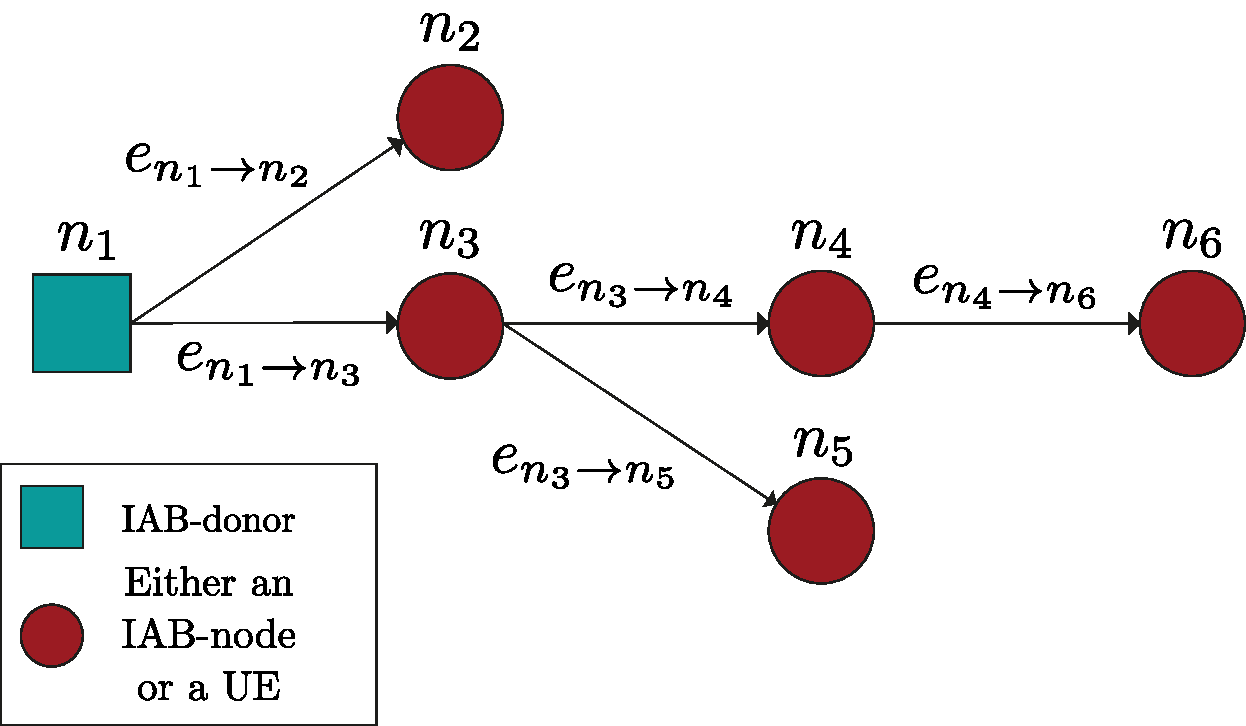
\includegraphics[width=0.7\linewidth]{Figures/CentralResourceManagement/IAB_Notation.pdf}}
    \caption{Comparison of the \gls{iab} network topologies analyzed in~\cite{3gpp_38_874} and related notation.}
    \label{Fig:IAB_top_not}
    % \vspace{-.6cm}  
\end{figure}

%TODO Explain scheduling and better formulation of the half-duplex explanation(e.g. the backhaul-aware)
Finally, the introduction of resource coordination mechanisms and related signaling is explicitly supported in the \gls{iab} specification drafts~\cite{3gpp_38_874, 3gpp_38_174}. Nevertheless, these solutions must reuse as much as possible the available NR specifications and
require at most minimal changes to the Rel.15 \gls{5gc} and \gls{nr}.

%According to these considerations, the remainder of this section will propose a generic algorithm for centralized access/backhaul resource partitioning which aims to be scalable, efficient and, in general, implementable in real-world deployments.

\subsection{System model}
\label{Subsec:sys_model}

According to these assumptions and referring to Fig.~\ref{Fig:IAB_notation}., a generic \gls{iab} network can be modeled as a directed graph $\mathcal{G} = \{\mathcal{N},  \mathcal{E} \}$, where the set of nodes $\mathcal{N} \mathop = \limits^{\Delta} \, \{ n_1, \, n_2, \, \ldots \, n_{\vert \mathcal{N} \vert }  \}$ comprises the \gls{iab}-donor, the various \gls{iab}-nodes and the \glspl{ue}. 
Accordingly, the set of directed edges $\mathcal{E} \mathop = \limits^{\Delta} \, \{ e_{1} , \, e_{2}, \, \ldots \, \allowbreak e_{\vert \mathcal{E} \vert} \} \equiv \{ e_{n_j \to n_k} \}_{j, k} $, where the edge $e_{n_j \to n_k}$ originates at the parent node $n_j$ and terminates at the children $n_k$, comprises in all the active cell attachments, either of mobile terminals to a \gls{gnb} or from \gls{iab}-nodes towards their parent node.
Since the goal of this paper is to study backhaul/access resource partitioning policies, this generic model can be actually simplified: in fact, all the \glspl{ue} connected to a given \gls{gnb} can be represented by a single node in $\mathcal{G}$ without any loss of generality. Similarly, the same holds true for their links toward the serving \gls{gnb}, which can then be represented by a single edge. 
%TODO Maybe mention that as a consequence the number of edges is significantly reduced, taking into consideration the expected # of UEs connected to a BS in 5G systems
Furthermore, this work focuses on \gls{st} topologies only. 

We define as \textit{feasible schedule} any set of links $\mathcal{E'} \subseteq \mathcal{E}$ such that none of them share a common vertex, i.e., $ \forall \, e_{n_j \to n_k} \neq e_{n_l \to n_m} \in \mathcal{E'}$ it holds that $n_{j} \neq n_{m}$ and $n_{l} \neq n_{k}$. Let then $f_u$ be a utility \textit{additive map}, namely, a function such that the overall utility experienced by the system when scheduling edges $e_1$ and $e_2$ satisfies $f_u (e_1, e_2) = f_u (e_1) + f_u(e_2)$. Let also $\mathcal{W} \mathop = \limits^{\Delta} \, \{ w_1, \, w_2, \, \ldots \, w_{\vert \mathcal{E} \vert } \}$ be the set of positive weights whose generic entry $w_j$ represents the utility which is obtained when scheduling the $j$-th edge, namely, $w_j \mathop = \limits^{\Delta} \, f_u (e_j)$. Then, the overall utility of the system is $\mathcal{U} \mathop = \limits^{\Delta} \, \sum_{e_k \, \in \, \mathcal{E'}} f_u(e_k) = \sum_{e_k \, \in \, \mathcal{E'}} w_k $.
The goal is to find the feasible set $\mathcal{E'}^{*}$ which maximizes the overall utility, i.e., $\underset{\mathcal{E'}}{\mathrm{argmax}} \,\, \mathcal{U} $. In computer science, this task is typically referred to as the \textit{Maximum Weighted Matching} problem~\cite{Korte2002}.

Finding the \gls{mwm} of a given graph, in the general case, is not trivial from a computational point of view. 
In fact, the fastest known \gls{mwm} algorithm for generic graphs has a complexity of \bigO{\vert V \vert \vert E \vert + \vert V \vert^2 \log{\vert V \vert}}~\cite{1990Gabow}, posing serious limitations to the suitability of such algorithm to \gls{5g} and beyond networks, which target a connection density of 1 million devices per km\textsuperscript{2}. However, we argue that under the aforementioned assumptions on the system model, which restrict the network to an \gls{st} topology, it is possible to design an \gls{mwm}-based semi-centralized resource partitioning framework which exhibits linear complexity with respect to the network size and which, as a result, is able to satisfy the scalability requirements highlighted by \gls{3gpp} in~\cite{3gpp_38_874}. 
Nevertheless, the proposed framework can be easily extended to the case of a \gls{dag} \gls{iab} network. In such regard, a sub-optimal strategy is to periodically discard, during each centralized allocation, the redundant edges of each node. In such a way, the input which is fed to the \texttt{T-MWM} algorithm is, effectively, an \gls{st}. A second, optimal extension can be obtained by computing at the controller the \gls{mwm} of the network via a generic \gls{mwm} algorithm, instead of using the \gls{st}-specific \texttt{T-MWM} as in the proposed framework. However, this strategy would feature a higher computational complexity.

\section{Semi-centralized resource allocation scheme for IAB networks}
\label{Sec:scheme_main}

This section presents an \gls{mwm} algorithm for \gls{st} topologies (Sec.~\ref{Sec:T-MWM}), an efficient and \gls{mwm}-based semi-centralized resource partitioning framework for \gls{iab} networks (Sec.~\ref{Sec:Cent-scheme}) and some considerations about its implementation (Sec.~\ref{Sec:ns3-impl}). 
Specifically, the proposed scheme collects at a controller installed on the \gls{iab}-donor L1 and/or L3 measurements from the various \glspl{gnb}. Then, it uses such information to build a weighted \gls{st} which represents the \gls{iab}-network. In particular, the network topology is inferred by examining the incoming parent-child associations. The edge weights are also computed from the received measurements, based on the specific policy (hence, of target \glspl{kpi}) of choice. Finally, the resource partitioning is optimized by computing an \gls{mwm} of the network and then prioritizing the links which comprise it. A high level diagram of is provided in Fig.~\ref{Fig:Diagram}.

\begin{figure}[t]
    \subfloat[IAB protocol stack and topology.\label{Fig:IAB-net}]{
    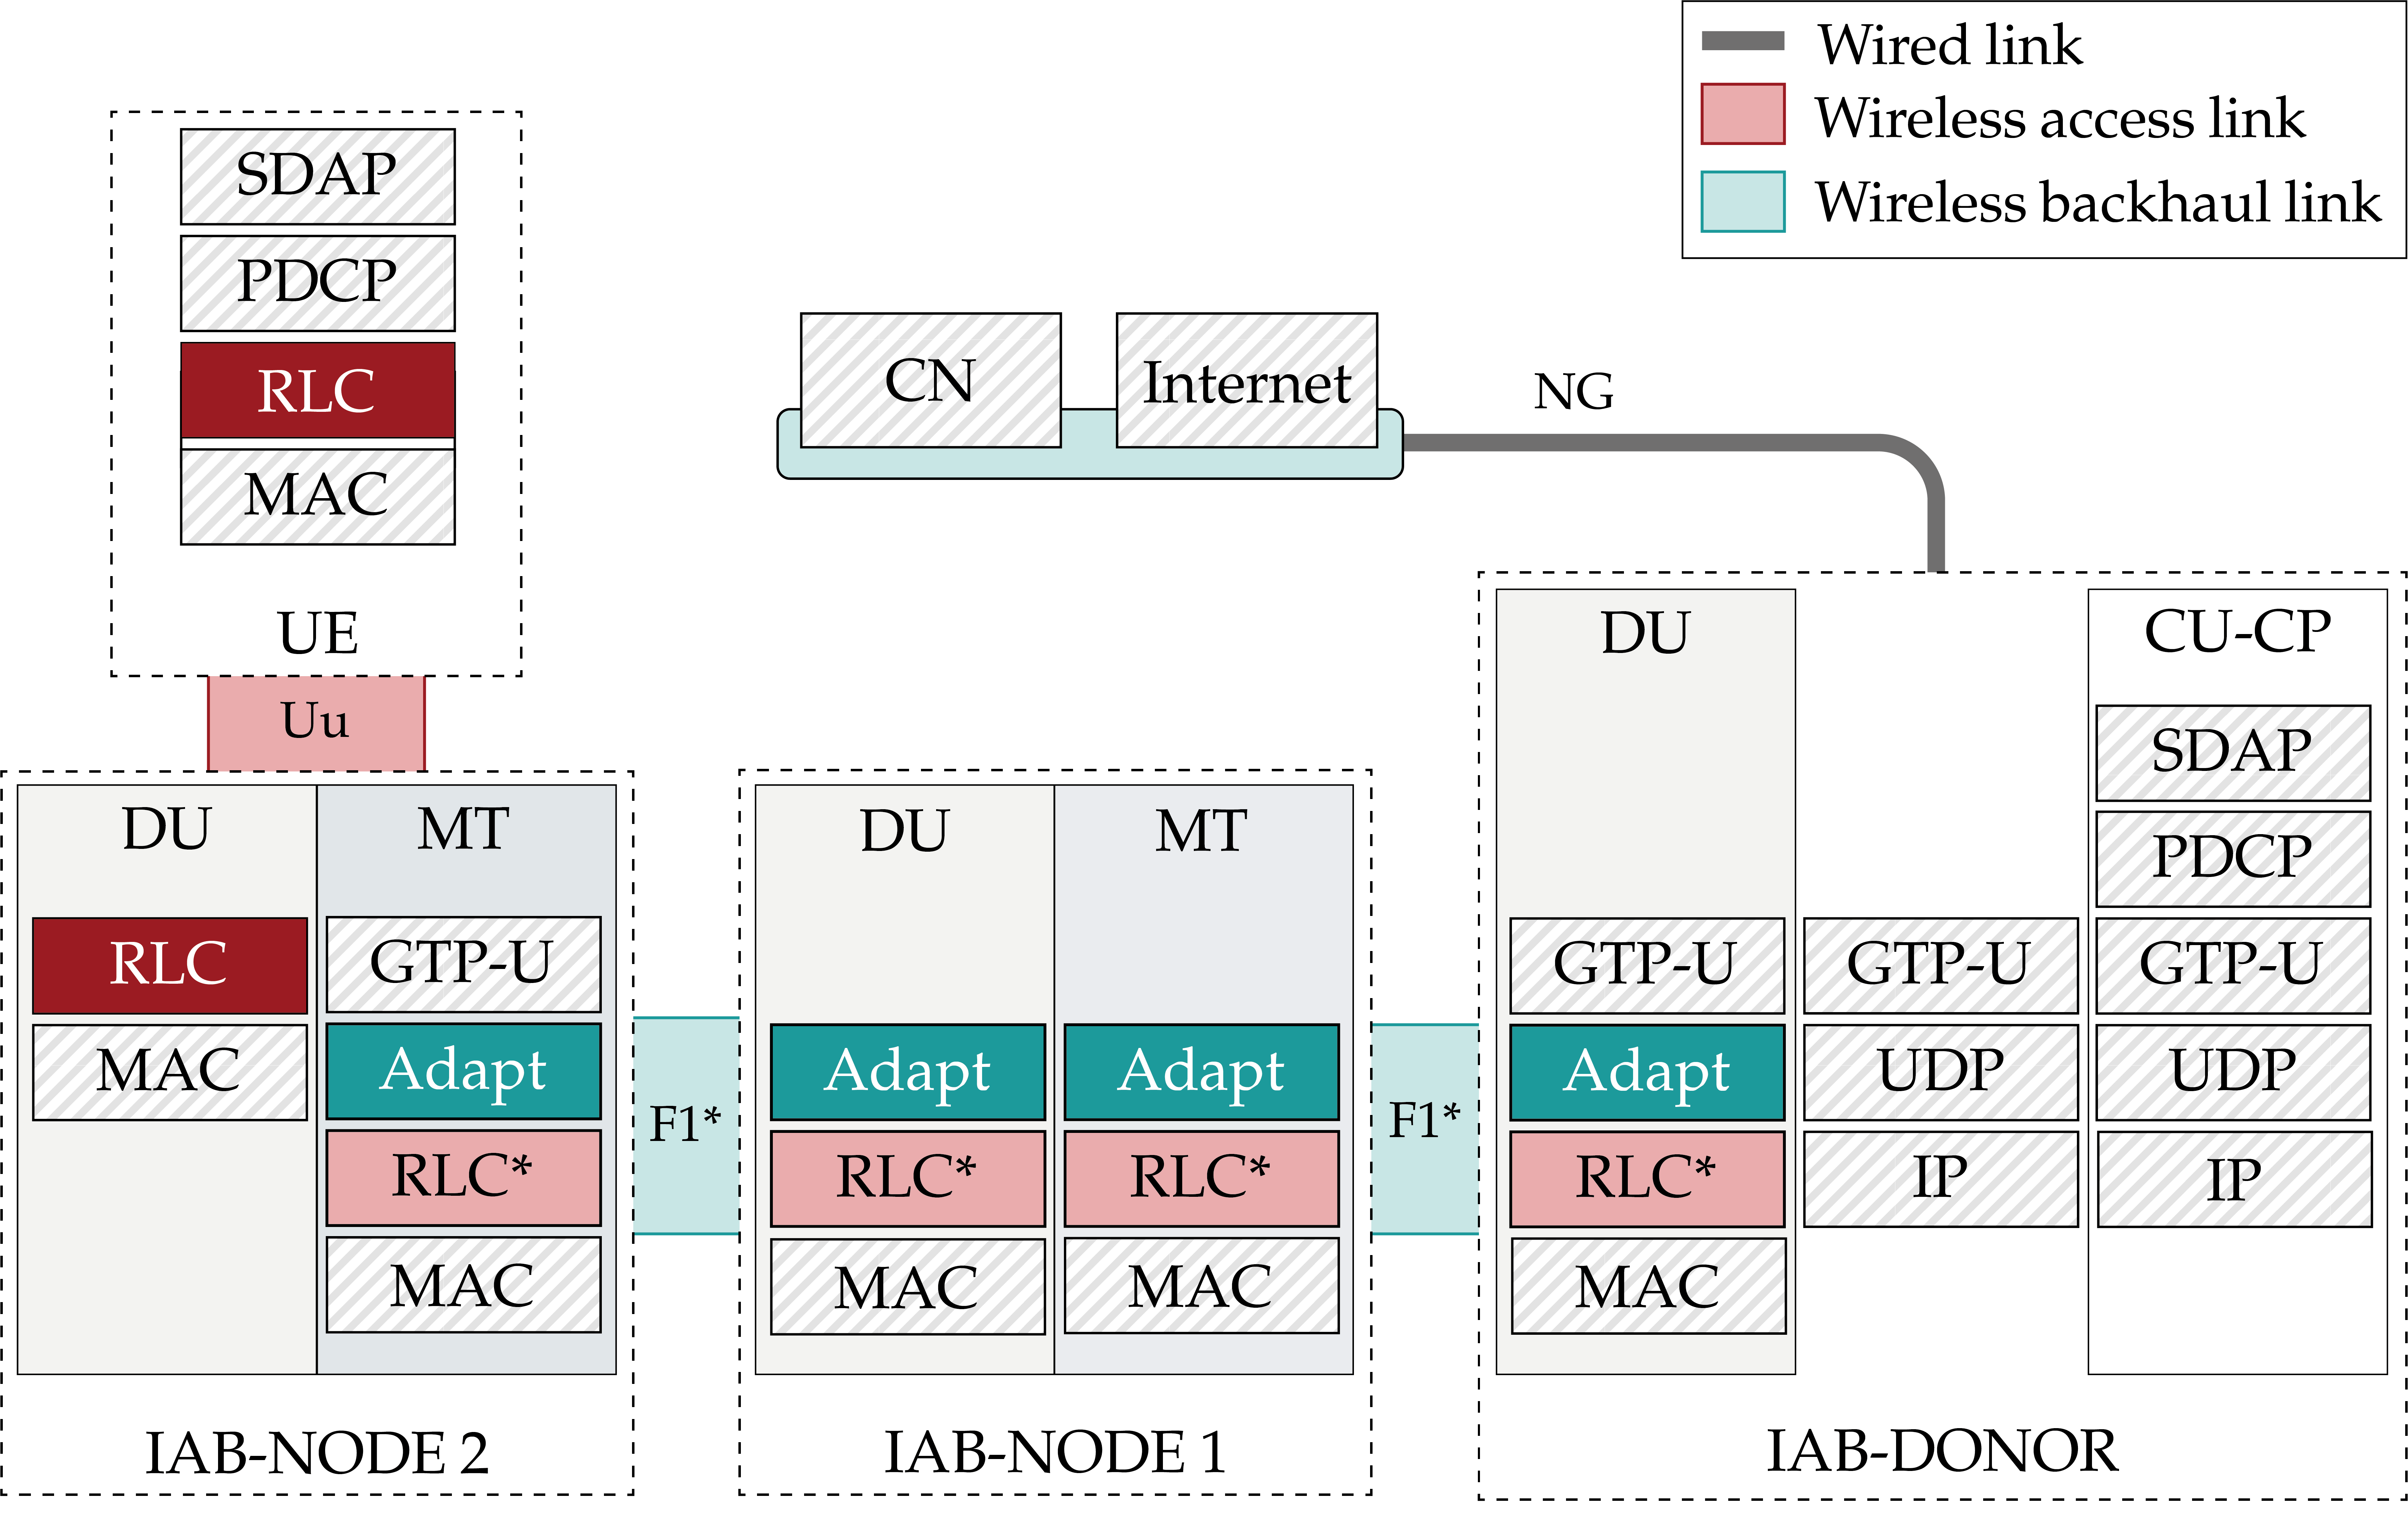
\includegraphics[width=0.95\linewidth]{Figures/CentralResourceManagement/architecture_full.png}}\hfill
    \subfloat[High level diagram of the proposed \gls{mwm}-based framework.\label{Fig:Diagram}]{
    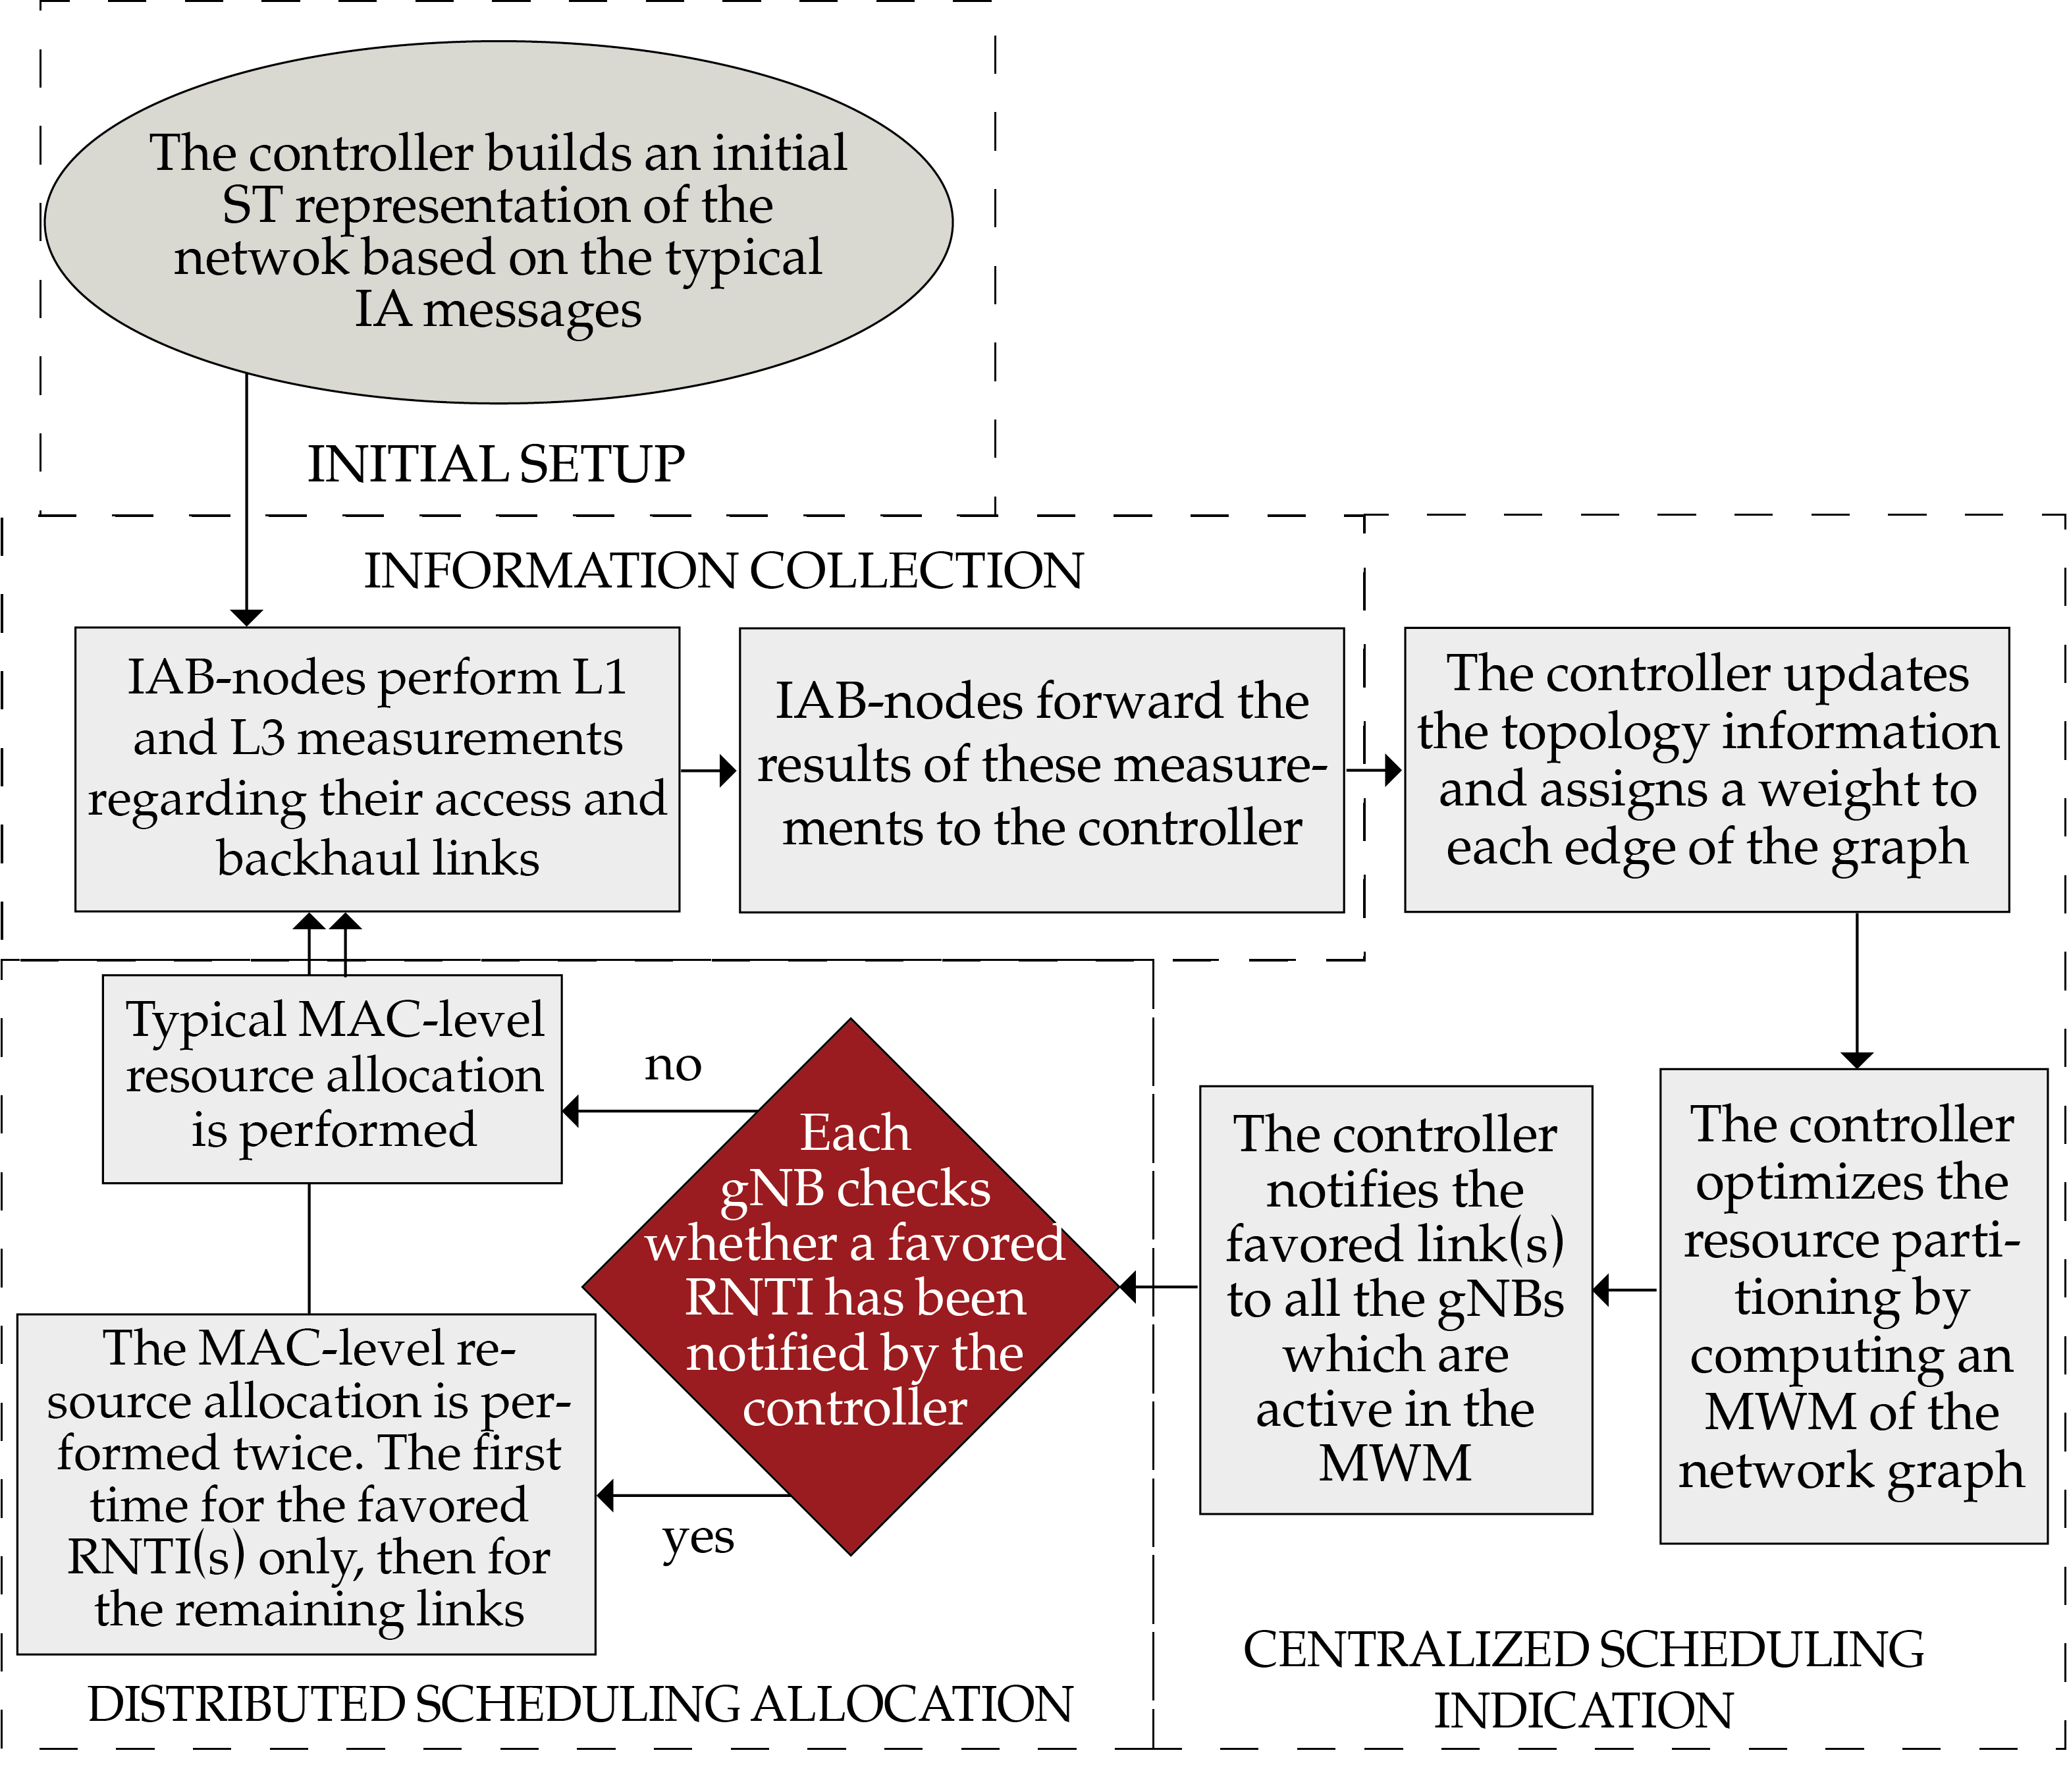
\includegraphics[width=0.95\linewidth]{Figures/CentralResourceManagement/FlowChart_IAB.png}}
    \caption{IAB topology and proposed MWM-based framework.}
    \label{fig:fr-top}
\end{figure}

\subsection{MWM for ST graphs}
\label{Sec:T-MWM}

As the first of our contributions, we present an algorithm, hereby called \texttt{T-MWM}, which computes the \gls{mwm} of an \gls{st} in linear time. In particular, \texttt{T-MWM} is a bottom-up algorithm which, upon receiving as input a weighted \gls{st} $\mathcal{G}$ described by its edge map $\mathbf{E}$ and the corresponding weight map $\mathbf{W}$, produces as output a set of active edges $\mathbf{E^*}$ which are an \gls{mwm} of $\mathcal{G}$. That is to say, $\mathbf{E^*}$ is a matching of $\mathcal{G}$ which yields the globally maximum utility.
Furthermore, $\mathbf{E}$ is from now on assumed to exhibit the following invariant: each \gls{iab} parent precedes its children in the map, hence avoiding the need for a recursion. 
%TODO can remove this when we add the discussion on the complexity of each phase
This is automatically obtained as each \gls{iab} child connects after its parent, and is thus added to the map in a subsequent position.
Nevertheless, this assumption can be easily relaxed, albeit at the cost of losing as a side-effect the bottom-up design.

%TODO rewrite, do not include what used to be Lemma 1.
% Needs a link between these two sections

The proposed algorithm is designed starting from the observation that, given the generic node $n_k \in \mathcal{G}$ and a matching $\mathbf{\bar{E}}$ of $\mathcal{G}$, we can identify the following mutually exclusive and collectively exhaustive cases: $\mathbf{\bar{E}}$ can contain either one or zero edges which originate from $n_k$. Based on this fact, we then discern the optimal utilities which can be obtained in each of these cases. Specifically, we define the maximum utilities yielded by a matching of $n_k$'s sub-tree which either contains a link originating from $n_k$ or not as $\mathbf{F}(n_k)$ and $\mathbf{G}(n_k)$, respectively.
Then, as can be seen in Alg.~\ref{Alg:tmwm}, the \texttt{T-MWM} algorithm basically consists in two traversals of the network graph. During the first one we compute the $\mathbf{G}$ and $\mathbf{F}$ functions for all the nodes in $\mathcal{G}$ using the recursive formulas provided by Lemma~\ref{lemma_utils}. Finally, during the second traversal, this knowledge is used for computing an \gls{mwm} of the network; the correctness of this last phase is proved by Lemma~\ref{lemma_active_edges}.

%Specifically, these formulas are based on the following observations.
%First, given the generic internal node $n \in \mathcal{G}$, any \gls{mwm} contains an edge which originates either from $n$ or one of its children, as stated in Lemma~\ref{lemma_ch_par}. It follows that if the \gls{mwm} does not contain any edge which originates from $n$, the maximum utility is achieved when activating \textit{all} the edges which originate from its children. On the other hand, whenever the edge from $n$ to its generic child $m$ is included in the \gls{mwm}, the
%All together, these first two Lemmas prove the correctness of the first part of Alg.~\ref{Alg:tmwm}.

%TODO Maybe rework edges notation here as well, in order to make it slightly more uniform
\begin{algorithm}[tbp!]
\small
    \caption{Tree-Maximum Weighted Matching}
    \label{Alg:tmwm}
    \hspace*{\algorithmicindent} \textbf{Input:} A weighted \gls{st} $\mathcal{G}$ encoded by a map $\mathbf{E}$, which associates each node in $\mathcal{G}$ to its edges, and the corresponding weights map $\mathbf{W}$. \\ 
    \hspace*{\algorithmicindent} \textbf{Output:} An \gls{mwm} $\mathbf{E^*}$ of $\mathcal{G}$. 
    \begin{algorithmic}[1] % The number tells where the line numbering should start
        \Procedure{\texttt{T-MWM}}{$\mathbf{E}, \mathbf{W}$} 
            \State $\mathbf{F} \gets \mathbf{0}$; $\mathbf{G} \gets \mathbf{0}$ \Comment{Initialize the utility vectors to zero vectors}
            \State $\mathbf{E^*} \gets \{ \}$ \Comment{Initialize the set of active edges as empty}
            \For{each internal node $n_k \in \mathbf{E}$} \Comment{\parbox[t]{.43\linewidth}{In ascending order w.r.t. to their depth in $\mathcal{G}$}}
            \State $maxUtil \gets - \infty$;  $\mathbf{maxUtilChild}(n_k) \gets \{ \}$
            \For{each edge $e_{n_k \to n_j} \in \mathbf{E}(n_k) $} \Comment{Iterate over its edges}
                \State $\mathbf{G}(n_k) \gets \mathbf{G}(n_k) + \max \left\{ \mathbf{F}(n_j), \mathbf{G}(n_j) \right\}$
                \State $currUtil \gets \mathbf{W} ( e_{n_k \to n_j} ) - \left[ \mathbf{F}(n_j) - \mathbf{G}(n_j) \right]^+  $
            \If{$currUtil > maxUtil$}
            	\State $maxUtil \gets currUtil$;  $\mathbf{maxUtilChild}(n_k) \gets n_j$ 
            \EndIf
            \EndFor\label{edgesFor}
            \State $\mathbf{F}(n_k) \gets \mathbf{G}(n_k) + maxUtil$ 
            \EndFor\label{nodesFor}
			
			\For{each internal node $n_k \in \mathbf{E}$} \Comment{\parbox[t]{.43\linewidth}{In ascending order w.r.t. to their depth in $\mathcal{G}$}}			
			
				\If { $\mathbf{F}(n_k) \geq \mathbf{G}(n_k)$}
					\State $\mathbf{E^*} \gets \mathbf{E^*} \cup e_{n_k \to \mathbf{maxUtilChild}(n_k)}$
					\State $\mathbf{F}(\mathbf{maxUtilChild}(n_k)) \gets -\infty$ \Comment{\parbox[t]{.3\linewidth}{Ensure child does not get activated multiple times}}
				\EndIf\label{activeIf}
			\EndFor\label{edgesFor2}            
            
            \State \textbf{return} $\mathbf{E^*}$
        \EndProcedure
    \end{algorithmic}
\end{algorithm}

%\begin{lem}
%\label{lemma_ch_par}
%Let $n_k$ be an arbitrary internal node of $\mathcal{G}$ and $\{ n_j \}_k$ be the set of its children. Then, any \gls{mwm} of $\mathcal{G}$ must contain an edge which has as one of its vertices either $n_k$ or an element of  $\{ n_j \}_k$.
%\end{lem}
%
%\begin{IEEEproof}
%Suppose there exists an \gls{mwm} $\mathbf{E^*}$ of $\mathcal{G}$ which does not contain any such edge. Then the set $\hat{\mathbf{E}}^* \mathop = \limits^{\Delta} \, \mathbf{E^*} \cup \{ e_{n_k \to n_m} \}$, where $ e_{n_k \to n_m} $ is the edge from $n_j$ to its (arbitrary) child $n_m$ is still a feasible activation set, since no edge in $\mathbf{E^*}$ shares such vertices. Furthermore, since the weights are positive we have that $f_u (\hat{\mathbf{E}}^*) = f_u (\mathbf{E^*}) + \mathbf{W} (e_{n_k \to n_m}) > f_u (\mathbf{E^*}) $, which is clearly a contradiction.
%\end{IEEEproof}

\begin{lem}
\label{lemma_utils}
Given an \gls{st} $\mathcal{G}$, consider its generic internal node $n_k$. Let then $\mathbf{F}(n_k)$ be the maximum utility yielded by a matching of $n_k$'s sub-tree which activates a link originating from $n_k$, and $\mathbf{G}(n_k)$, conversely, the utility provided when such matching contains no links which feature $n_k$ as parent. Then, we have that:
\[ 
\begin{cases}
\mathbf{G}(n_k) = \sum\limits_{ \{ n_j \}_k} \max \left\{ \mathbf{F}(n_j), \mathbf{G}(n_j) \right\} \\

\begin{aligned}
\mathbf{F}(n_k) &= \mathbf{G}(n_k) + \underset{\{ n_j \}_k }{\max} \{ \mathbf{W} ( e_{n_k \to n_j} ) \\
&- \left[ \mathbf{F}(n_j) - \mathbf{G}(n_j) \right]^+ \}
\end{aligned}


\end{cases}
\]
where the set $\{ n_j \}_k$ comprises all the children of $n_k$ and $\left[ x \right]^+ = \max\{x, 0\}$ is the positive part of $x$.
%
Conversely, for leaf nodes $n_l$ it holds that $\mathbf{F}(n_l) \equiv \mathbf{G}(n_l) \equiv 0 $.
\end{lem}

\begin{proof}
This lemma can be proved by induction over the height $h_k$ of the sub-tree corresponding to node $n_k$. The base case is $h_k = 0$, i.e., when $n_k$ is a leaf node; in this case, trivially, both $\mathbf{F}(n_k)$ and $\mathbf{G}(n_k)$ are zero since no links exhibit $n_k$ as parent node and the sub-tree of $\mathcal{G}$ which originates in $n_k$ consists of $n_k$ only, respectively.

Then, assume that $n_k$'s sub-tree exhibits a generic height $h_k > 0$, and that the above formulas hold for each of its children sub-trees, which exhibit a height $h_j < h_k$. If we do not activate any edge which originates from $n_k$, then no added constraints are introduced concerning the edges which can be activated in its children sub-trees. Therefore, %the maximum utility achieved by any matching of $n_k$'s sub-tree, without activating any node which originates from $n_k$, 
$\mathbf{G}(n_k)$ is simply the sum of the utilities achieved by any \gls{mwm} computed on its children sub-trees, i.e.,  $\mathbf{G}(n_k) = \sum\limits_{ \{ n_j \}_k} \max \left\{ \mathbf{F}(n_j), \mathbf{G}(n_j) \right\}$.
The remaining option is to activate exactly one edge, hereby called $e_{n_k \to n_m}$, which originates from $n_k$. In this case, no additional edges which feature $n_m$ as parent can be added to the matching. As a consequence, the contribution of $n_m$'s sub-tree on $\mathbf{F}(n_k)$ reads $\mathbf{G}(n_m)$. Conversely, no additional constraints are introduced regarding the other nodes. It follows that the utility obtained in this instance reads:
\[ \sum_{ \{ n_j \neq n_m\}_k } \max \left\{ \mathbf{F}(n_j), \mathbf{G}(n_j) \right\} +  \mathbf{W} ( e_{n_k \to n_m} ) + \mathbf{G}(n_m) \]
and can be rewritten as:
\[  \mathbf{G}(n_k) + \mathbf{W} ( e_{n_k \to n_m} ) - \left[ \mathbf{F}(n_m) - \mathbf{G}(n_m) \right]^+ \]
Finally, such utility is clearly maximized when $n_m$ is chosen as $ \underset{ \{ n_j \}_k }{\mathrm{argmax}} \, \{ \mathbf{W} ( e_{n_k \to n_j} ) - \left[ \mathbf{F}(n_j) - \mathbf{G}(n_j) \right]^+ \}$, yielding:
\[ \mathbf{F}(n_k) = \mathbf{G}(n_k) + \underset{\{ n_j \}_k }{\max} \, \{ \mathbf{W} ( e_{n_k \to n_j} ) - \left[ \mathbf{F}(n_j) -  \mathbf{G}(n_j) \right]^+ \} \qedhere \] 
\end{proof}

\begin{lem}
\label{lemma_active_edges}
Given an \gls{st} $\mathcal{G}$ of root $n_r$ and the $\mathbf{F}$ and $\mathbf{G}$ functions computed as per Lemma~\ref{lemma_utils}, an \gls{mwm} $\mathbf{E^*}$ of $\mathcal{G}$ can be computed by performing the following procedure:
%, in a recursive fashion
\begin{enumerate}
\item If $ \, \mathbf{F}(n_r) \geq \mathbf{G}(n_r) $, add to $\mathbf{E^*}$ the edge from $n_r$ to $n_m$, where the latter is defined as $n_m \mathop = \limits^{\Delta} \, \underset{ \{ n_j \}_r }{\mathrm{argmax}} \, \{ \mathbf{W} ( e_{n_r \to n_j} ) - \left[ \mathbf{F}(n_j) - \mathbf{G}(n_j) \right]^+ \}$. Then, repeat recursively on all the sub-trees corresponding to $n_r$'s children $\{ n_j\}_r \, \vert \, n_j \neq n_m$ and on the children of $n_m$ itself.
\item If $ \, \mathbf{F}(n_r) < \mathbf{G}(n_r) $, repeat recursively on all the sub-trees corresponding to $n_r$'s children.
\end{enumerate}
\end{lem}

%TODO Add more details
\begin{proof}
The above procedure always yields a feasible activation, i.e., a matching of $\mathcal{G}$.  In particular, in either options we never recurse on a node which has already been activated, hence no pair of edges $\in \mathbf{E^*}$ can share any vertices. Furthermore, due to the properties of $\mathbf{F}$ and $\mathbf{G}$, whenever $\mathbf{F}(n_r) \geq \mathbf{G}(n_r)$ a matching yielding maximal utility can be obtained by activating the edge $e_{ n_r \to n_m }$, where $n_m \mathop = \limits^{\Delta} \, \underset{ \{ n_j \}_r }{\mathrm{argmax}} \, \{ \mathbf{W} ( e_{n_r \to n_j} ) - \left[ \mathbf{F}(n_j) - \mathbf{G}(n_j) \right]^+ \}$.
Since the procedure is then recursively repeated on $n_r$'s children and the validity of $\mathbf{F}$ and $\mathbf{G}$ properties holds for each sub-tree in $\mathcal{G}$, the set of edges $\mathbf{E^*}$ produced by the above procedure comprise a \textit{maximal} matching, i.e., they yield the maximum possible utility among all the feasible schedules. 
\end{proof}

%TODO consider moving this paragraph to the framework steps, together with the complexity and overhead considerations provided in the review for all the framework steps
Regarding the computational complexity of the proposed algorithm, it can be observed that during the first phase the main loop effectively scans each edge of $\mathcal{G}$, hence exhibiting a complexity \bigO{\vert \mathbf{E} \vert}. Moreover,
the second phase of \texttt{T-MWM} has complexity \bigO{\vert \mathbf{V} \vert}, since it loops through all the network nodes.
Therefore, we can conclude that the overall asymptotic complexity of the algorithm is \bigO{\vert \mathbf{V} \vert + \vert \mathbf{E} \vert}, or, equivalently, \bigO{\vert \mathbf{V} \vert} since in an \gls{st} the number of edges equals $\vert \mathbf{V} \vert - 1$.

\subsection{Semi-centralized resource partitioning scheme}
\label{Sec:Cent-scheme}
Based on the system model introduced in Sec.~\ref{Sec:Sys-model}, and the \texttt{T-MWM} algorithm, we present a generic optimization framework which partially centralizes the backhaul/access resource partitioning process, in compliance with the guidelines of~\cite{3gpp_38_874}. 
The goal of this framework is to aid the distributed schedulers, adapting the number of \gls{ofdm} symbols allocated to the backhaul and access interfaces to the phenomena which exhibit a sufficiently slow evolution over time, i.e., large scale fading and local congestion. % Maybe mention also effectiveness of centralized is exarcebated by TDD constraints
This optimization is undertaken with respect to a generic additive utility function $f_u$. An \gls{iab} network of arbitrary size is considered, composed of a single \gls{iab}-donor, multiple \gls{iab}-nodes and a (possibly time-varying) number of \glspl{ue} which connect to both types of \glspl{gnb}. %TODO Ask Tommaso/Michele 
%The choice of neglecting cooperation among neighboring sectors is motivated by the fact that different \gls{iab}-donors are likely to be separated by a distance which is significantly greater than their respective coverage area (in fact, if this would not be the case, there would not be the need for \gls{iab} in the first place). % Not impossible, but arguably sub-optimal
%Therefore, we deem an inter \gls{iab}-donors resource coordination to be an unrealistic scenario, which as a consequence is out of the scope of this paper.
%TODO But wired info exchange is actually possible (X2), needs further work or remove entirely 
Furthermore, %let the topology of the \gls{iab} network be pre-computed, for instance by using the policies of~\cite{polese2018iab}, and 
assume that a central controller is installed on the \gls{iab}-donor. 

The proposed framework can be subdivided into the following phases, which are periodically repeated every $T_{alloc}$ subframes:
\begin{enumerate}
\item \label{Enum_frameword:item_one} \textbf{Initial setup}. This step, which is depicted in Fig.~\ref{Fig:Phase0}, consists in the computation of the simplified \gls{iab} network graph $\mathcal{G} \equiv \{ \mathcal{V}, \mathcal{E} \}$. Specifically, after this phase $\mathcal{V}$ comprises the donor and the various \gls{iab}-nodes. Accordingly, $\mathcal{E}$ contains their active cell associations.

\item \label{Enum_frameword:item_two} \textbf{Information collection}. During this phase, the various \gls{iab}-nodes send to the central controller a pre-established set of information for each of their children in $\mathcal{G}$. For instance, this feedback may consist in their congestion status and/or  information regarding their channel quality. To such end, the implementation of this paper uses modified versions of pre-existing \gls{nr} Release 16 \glspl{ce}, as strongly recommended in the \gls{iab} SI~\cite{3gpp_38_874}. However, the scheme does not actually impose any limitations in such regard.
\item \label{Enum_frameword:item_three} \textbf{Centralized scheduling indication}. Upon reception of the feedback information, the central controller updates $\mathcal{G}$ by inspecting the received node-parent associations. Then, the set of weights $\mathcal{W}$ is calculated and an \gls{mwm} of $\mathcal{G}$ is computed, using the \texttt{T-MWM} algorithm. The output of this procedure is the activation set $\mathbf{E^*}$, which yields a globally optimum solution with respect to the chosen utility function. Subsequently, $\mathbf{E^*}$ is used as to create a set of \textit{favored} downstream nodes, i.e., of children which will be served with the highest priority by their parent, as depicted in Fig.~\ref{Fig:Phase2}. Finally, these scheduling indications are forwarded to the various \gls{iab}-nodes which act as parents in the edges of $\mathbf{E^*}$.

\begin{figure}[tbp]
	\centering
	%\captionsetup{singlelinecheck=false, justification=justified}
  % this sets the width of the figure, adjust to your needs
  	\subfloat[The original topology, exhibiting the actual cell attachments, is depicted on the left. Conversely, the reduced one is shown on the right.\label{Fig:Phase0}]{
  	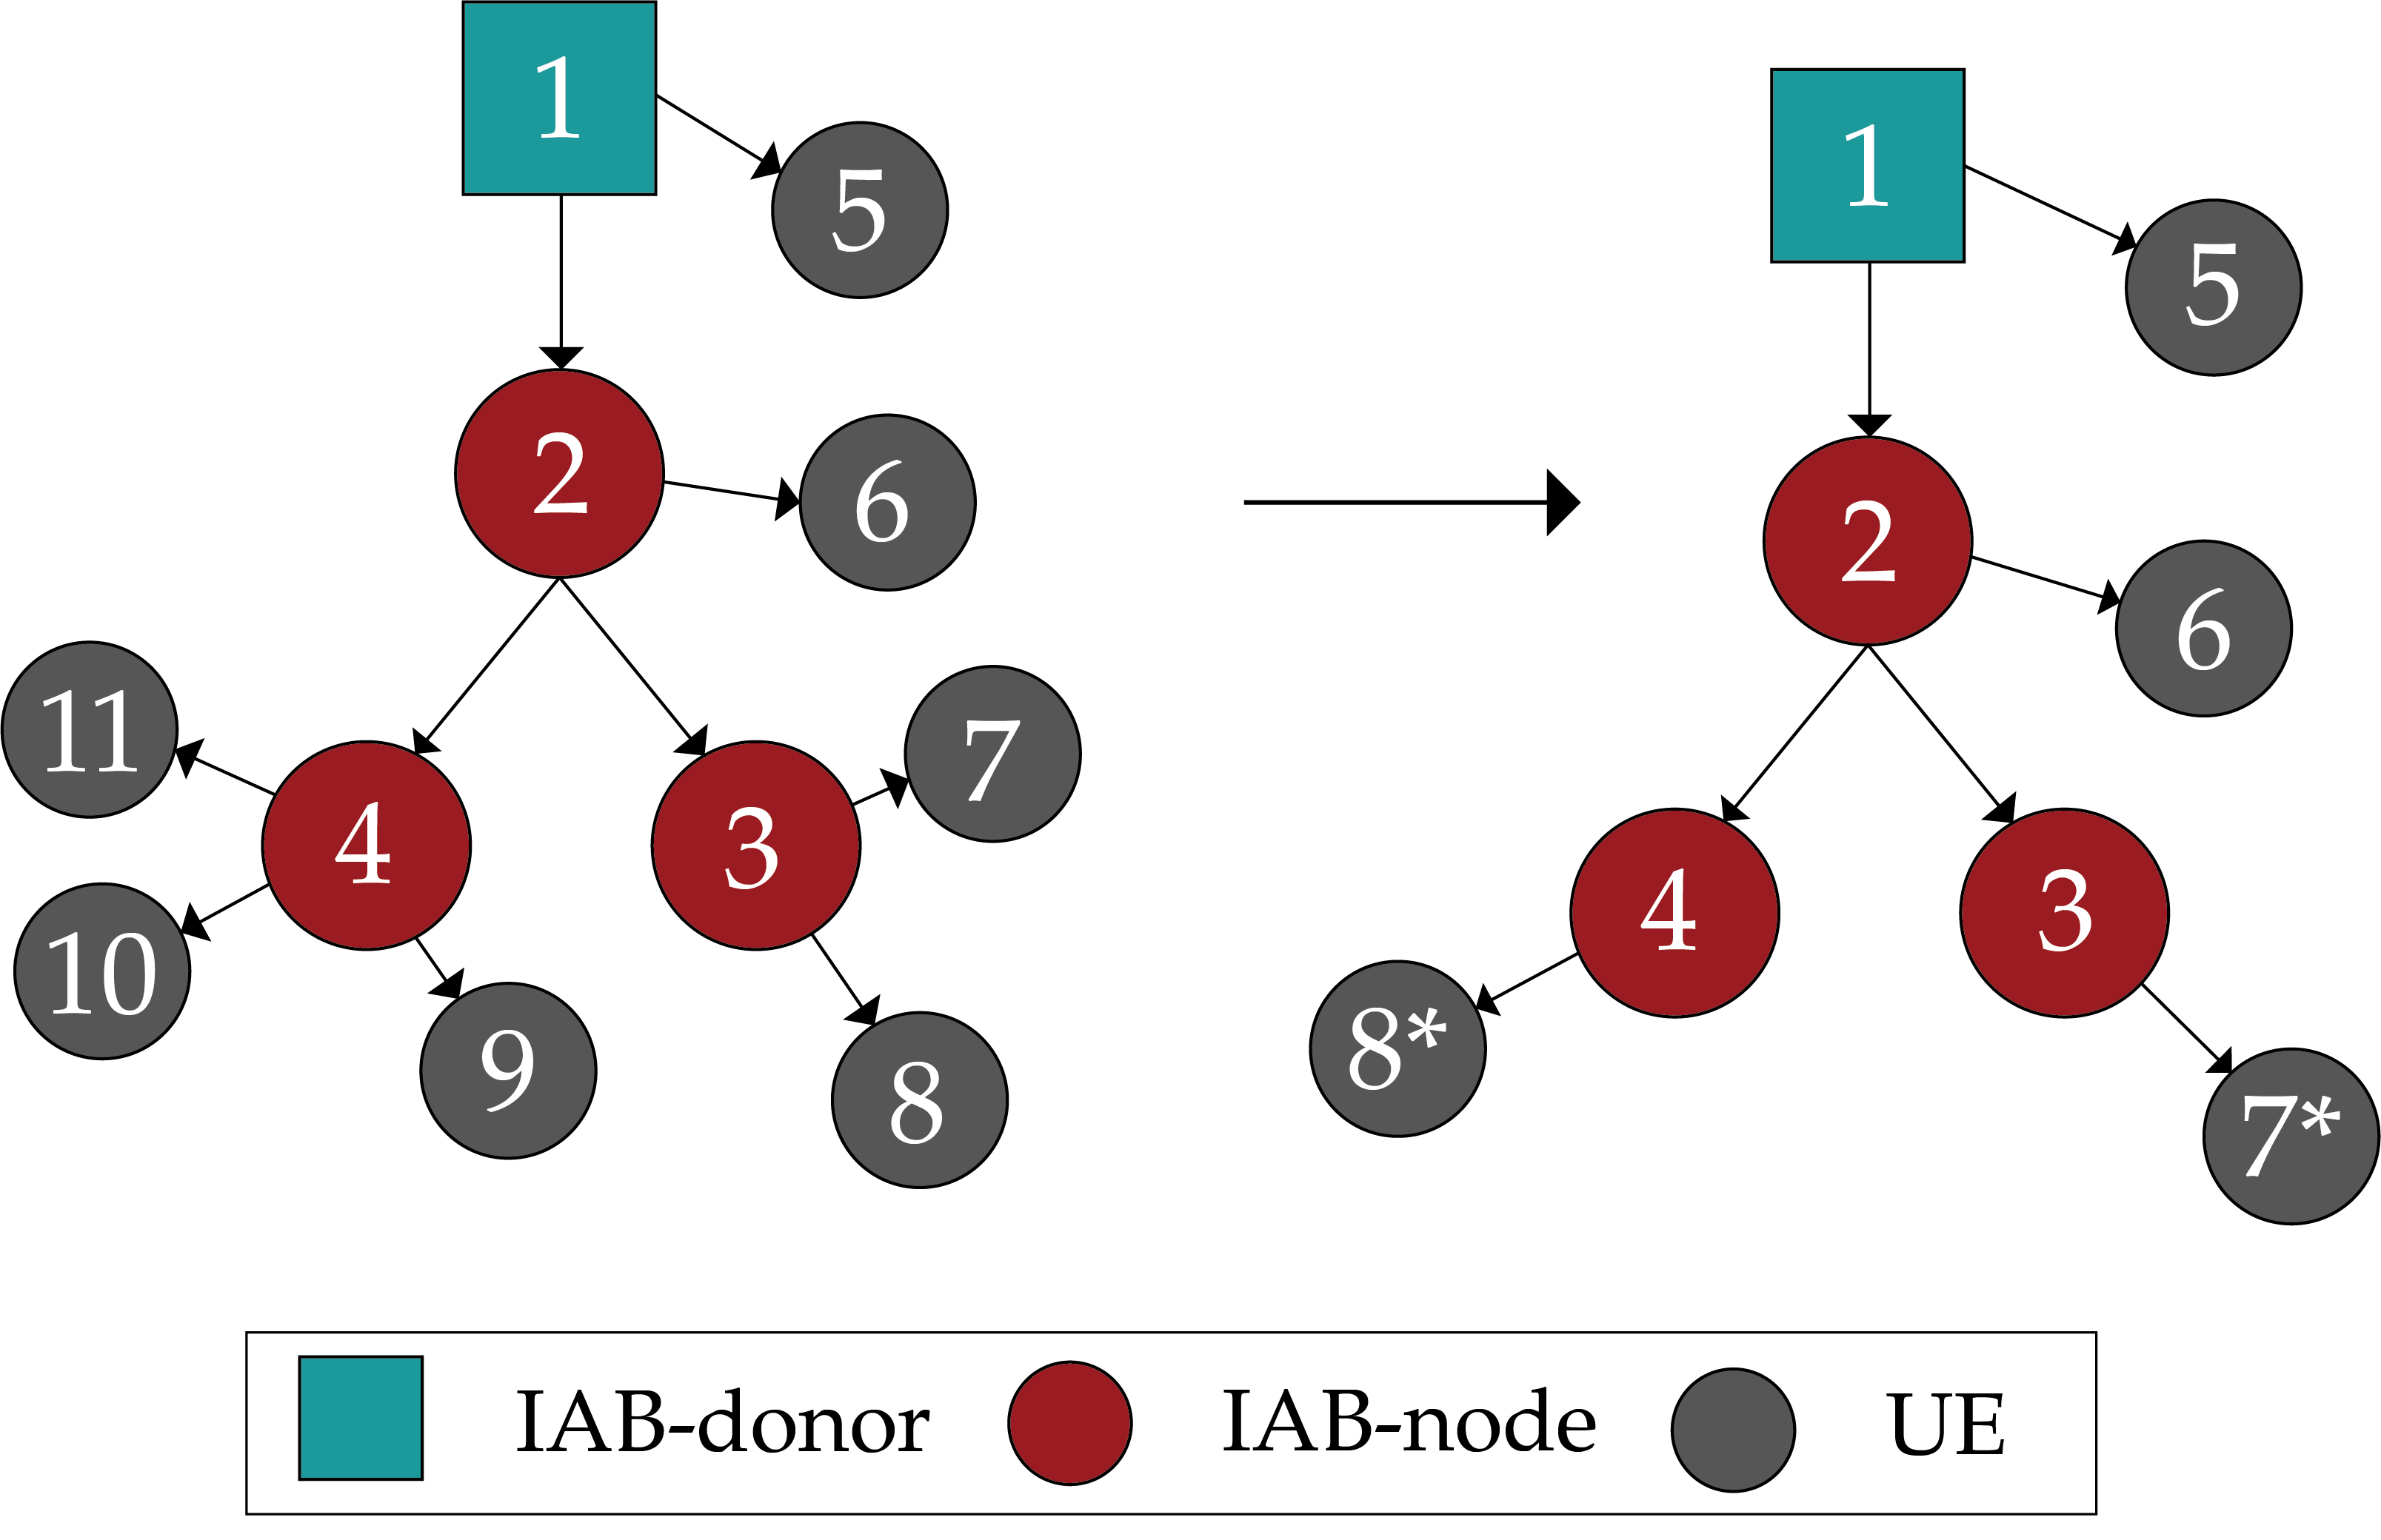
\includegraphics[width=0.7\linewidth]{Figures/CentralResourceManagement/Phase0.png}
    }\hfill
  	\subfloat[Computation of the \gls{mwm} and of the corresponding scheduling indications.\label{Fig:Phase2}]{
  	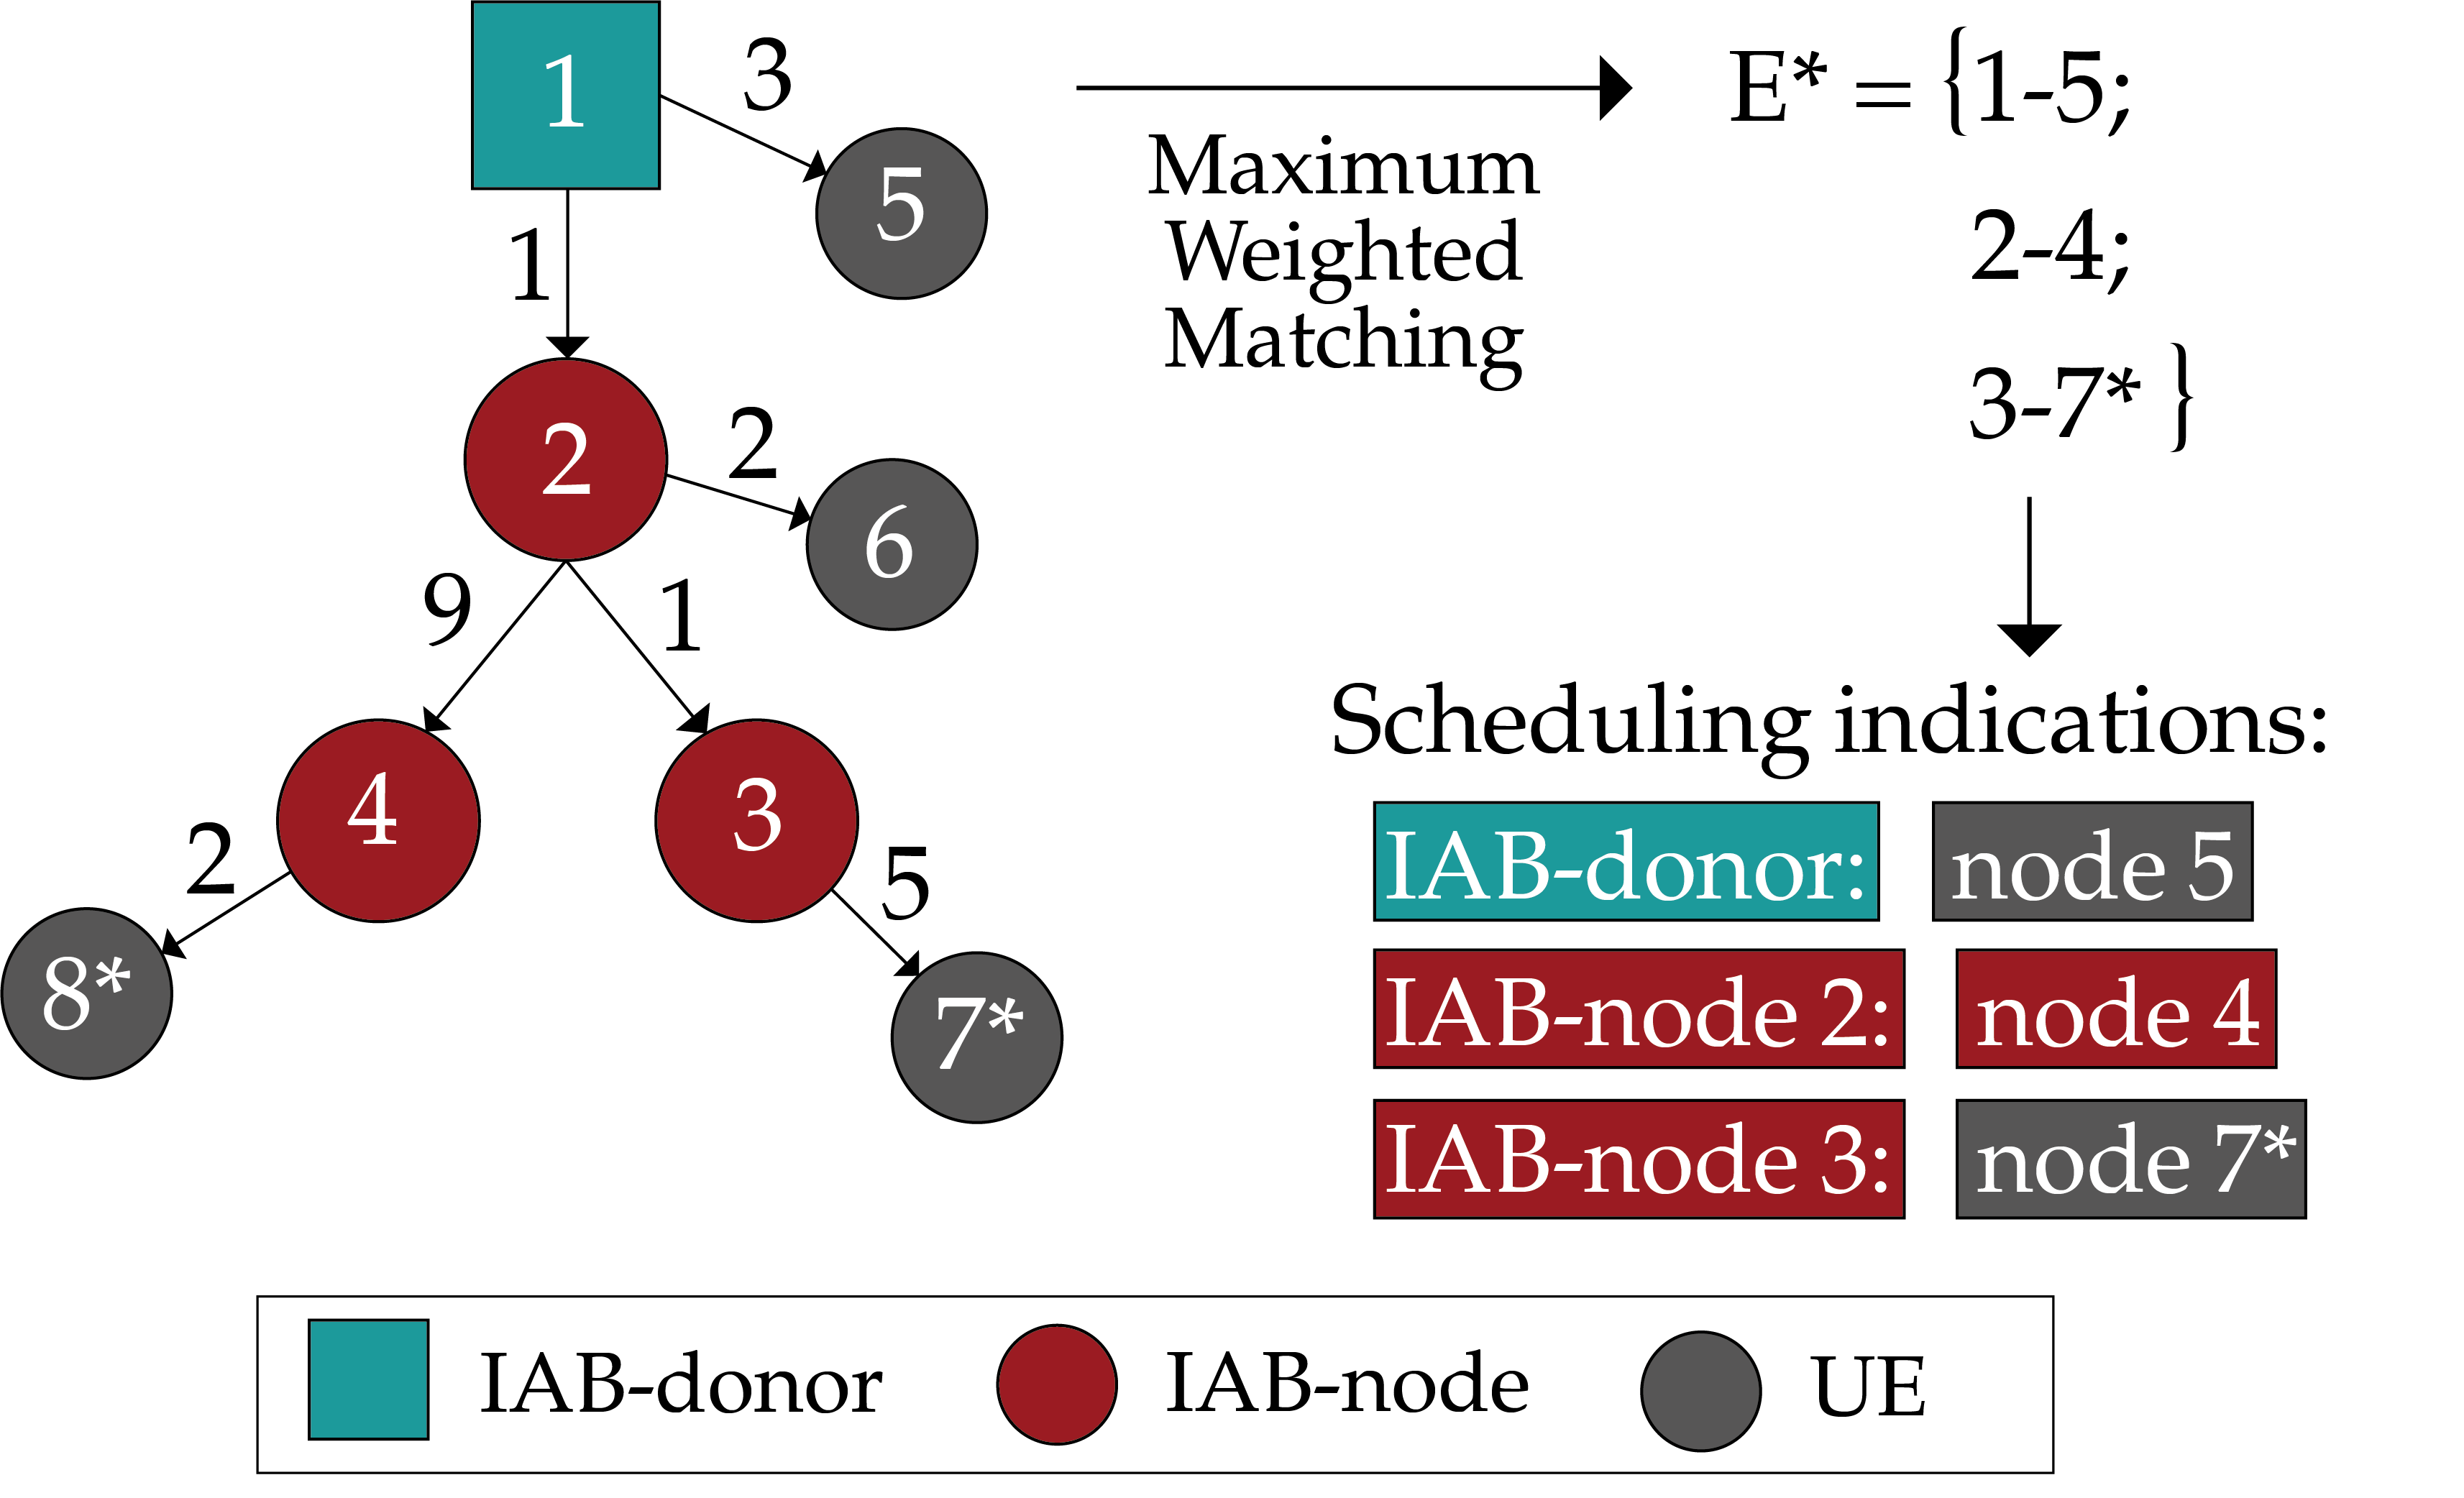
\includegraphics[width=0.7\linewidth]{Figures/CentralResourceManagement/Phase2.png}
    }
    \caption{High level scheme of the initial setup and centralized scheduling indication phases.}
    \label{Fig:Phases}
    %\vspace{-.6cm}  
\end{figure}


\item \textbf{Distributed scheduling allocation}. During this phase, the various \gls{iab}-nodes make use of the indications received by the central controller, if available, in order to perform the actual scheduling (which is, therefore, predominantly distributed). Specifically, the favored nodes are served with the highest priority, while the remaining downstream nodes are scheduled if and only if the resource allocation of the former does not exhaust the available \gls{ofdm} symbols.
\end{enumerate}
It is important to note that since $\mathcal{G}$ contains only the \gls{iab}-nodes, the donor and at most one ``representative" \gls{ue} per \gls{gnb}, the proposed scheme effectively performs only the backhaul/access resource partitioning in a centralized manner. On the other hand, the actual \gls{mac}-level scheduling is still undertaken in a distributed fashion, albeit leveraging the indications produced by the central controller. The major advantages which this two-tier design exhibits, compared to a completely centralized solution, are the presence of a relatively light signaling overhead and the ability to promptly react to fast channel variations, for instance caused by small scale fading.  

\subsection{Implementation of semi-centralized allocation schemes in mmWave IAB networks}
\label{Sec:ns3-impl}

The remainder of this section discusses how the proposed scheme can be implemented in \gls{iab} deployments, with references to how the \gls{3gpp} specifications can support it. Moreover, an in-depth analysis of the framework's communication overhead and computational complexity is provided. To such end, let $\mathcal{G} = \{ V, E \}$ be the reduced network graph, computed as per Sec.~II-C, and, conversely, let $\mathcal{\bar{G}} = \{ \bar{V}, \bar{E} \}$ comprise all the nodes in the \gls{iab} network.
% presents an implementation of the proposed scheme in the network simulator ns-3, along with considerations on its implementation in real world deployments.

In general, the resource allocation framework requires (i) a central controller, which is installed on the \gls{iab}-donor, or could be deployed in a \gls{ric} following the O-RAN architecture~\cite{bonati2020open}; and (ii) a scheduler which exchanges resource coordination information with the former. %and computes the weights for the resource allocation.
In particular, and referring to the aforementioned phases of the proposed scheme, the following %communication overhead, computational complexity and implementation  
additional considerations can be made. 

% Might be of interest and/or relevant
% In particular, \gls{rlc} bearers are independently setup for each hop in the \gls{iab}-network and an above-\gls{pdcp} adaptation layer forwards the various packet to either the access or the backhaul \gls{pdcp}s. Therefore, \textit{MmWaveIabNetDevice}s exhibit all the L2 \gls{5g} stack layers up to and including the latter, as can be seen in Fig.~\ref{Fig:mmWaveIabNetDevice}.

\subsubsection{Initial setup}
%The setup of the various centralized mechanisms is subdivided into two sub-phases: an initial configuration, where the relevant entities are initialized, and a periodic update of the topology information.
%The initial configuration . 
During this phase, which takes place when the \gls{iab}-nodes perform their first connection to the network, the controller acquires preliminary topology information by leveraging the configuration messages which are already exchanged during the typical Rel.16 \gls{ia} procedure~\cite[Sec. 9.6]{3gpp_38_874}. Therefore, no additional overhead is introduced. 
Specifically, a map which associates each \gls{iab}-node in the network to a list of its edges, identified by global identifiers (which from now on will be referred to as ``IDs"), is computed. %Since this phase takes place when no \gls{ue} has performed its \gls{ia} procedure yet, the exchanged topology information concerns the donor and \gls{iab}-nodes only.
As a consequence, $\mathcal{O} \left( \vert V \vert \right) $ insertions in a sorted map are performed and this one-time setup exhibits a computational complexity of $\mathcal{O} \left( \vert V \vert \log( \vert V \vert ) \right) $.

\subsubsection{Information collection}
The generation of the feedback information is performed in a distributed manner by  the \glspl{gnb}. To such end, the current implementation features the forwarding of information on the channel quality and buffer status, in the form of \glspl{cqi} and \glspl{bsr} respectively. This choice is driven by both the will of maximizing the re-utilization of the \gls{nr} Rel.16 specifications and the goal of making use of \gls{mac}-level \glspl{ce} only, hence avoiding the introduction of any constraint regarding the supported \gls{iab}-relaying architecture.
% Not so relevant for real deployments
%This periodic feedback to the controller is started by the \texttt{Do\-Sched\-Trigger\-Req} method of the various \texttt{MmWave\-RrIab\-Mac\-Scheduler} instances, which in turn calls the \texttt{Gen\-Cumulative\-Map} methods each subframe. However, the central controller can periodically discard the received feedback; by leveraging this possibility, the information collection can be configured to exhibit a period of $T_{collect} > 1$ subframes. 
In particular, the \gls{cqi} and \gls{bsr} information is generated by analyzing the corresponding \glspl{ce}, which are already received by the scheduler of each \gls{gnb}, and checking whether the source \gls{rnti} belongs to an \gls{iab}-node or to a \gls{ue}. In the first case, the corresponding ID
%\footnote{This change of identifiers is extremely important, as \gls{rnti}s are unique only within the scope of the \gls{gnb} they are attached to. Conversely, the IDs are globally unambiguous by design, hence suited for identifying terminals which may be connected to different \gls{gnb}s. \textbf{TODO: is this footnote necessary?}} 
is retrieved and an entry carrying such identifier along with its \gls{cqi}/\gls{bsr} value is generated. 
The feedback information concerning the \glspl{ue}, instead, is averaged in the case of the \glspl{cqi} and added up for the \glspl{bsr}, to obtain a single value for each \glspl{gnb}.
%It can be noted that both \glspl{cqi} and \glspl{bsr} are available to the scheduler, since the UL buffer statuses are already periodically reported by the downstream nodes via their \gls{bsr}s and the DL statuses can be easily retrieved by the former, since the \gls{rlc} buffers reside on the same node as the scheduler itself, i.e., the \gls{gnb}.

Referring to the \gls{3gpp} specifications of~\cite{3gpp_38_321}, the buffers occupancy can then be forwarded to the \gls{iab}-donor by introducing a Short \gls{bsr}, which carries a single \gls{lcg} ID and its respective buffer size. This is motivated by the fact that we do not keep track of per-flow information, i.e., we aggregate all the different \gls{rlc} bearers into a single measurement report. 
Similarly, the channel qualities can be reported by the various \gls{iab}-nodes via an additional \gls{cqi}-only \gls{csi} report, based on a \gls{wb} measurement. Therefore, we can upper bound the size of these \glspl{ce} as 11~\cite{3gpp_38_321} and 7 bits~\cite{3gpp_r1_1713763} respectively. 
%Both additional \glspl{ce} leverage pre-existing \gls{nr} measurements: the main novelty would be the introduction of their periodic reporting to the \gls{iab}-donor. 
%To such end, the \gls{5g} \gls{cqi} and \gls{bsr} data-structures require an additional field which carries the ID, if the chosen \gls{iab}-relaying architecture does not feature an Adaptation Layer~\cite{3gpp_38_874}. Conversely, relaying solutions which support the latter can reuse the \gls{nr} \glspl{ce} and let such layer introduce an additional header.
Regarding the computational complexity, in this phase we generate, at each \gls{gnb}, one \gls{cqi} and one \gls{bsr} for each backhaul link, and (possibly) compute one cumulative \gls{cqi} and \gls{bsr} for the \glspl{ue}. Therefore, the asymptotic complexity of this phase can be identified as $ \mathcal{O} \left(\vert V \vert \right)$.

\subsubsection{Centralized scheduling indication}
\label{Sec:cent_indic}
During this phase, the controller makes use of the feedback received from the \glspl{gnb} to update the topology information, compute the weights of the various network links and to generate the centralized scheduling indications. 

Regarding the former, no additional control information is required. In fact, the periodic feedback received from the various \gls{iab}-nodes, which carries a list of ID-value pairs, can be used in such regard. In particular, the controller checks the child-parent associations for discrepancies with its local knowledge, and, if so, updates the stored associations. Discrepancies can arise under two circumstances: the connection of the first \gls{ue} to an \gls{iab}-node and the handover to a different parent of any \gls{iab}-node. In the first case, just the corresponding ``cumulative access node'' needs to be added to the aforementioned map. On the other hand, whenever a backhaul link changes, the topological information for the whole subtending tree must be updated. Since in the worst case this might require an update of the whole map, the asymptotic complexity of the topology information update is $\mathcal{O} \left( \vert V \vert \right) $. Thanks to this periodic update, our framework is robust with respect to \glspl{rlf} and handovers, which may occur due to blockages or mobility of \glspl{ue} and, possibly, \glspl{gnb}.

With respect to the computation of weights for the \gls{mwm} problem, we propose the following policies:

\begin{enumerate}
\item \textbf{\gls{msr}}. 
This policy maximizes the overall \gls{phy}-layer throughput, i.e., the utility function is 
\[ f_u^{\mathrm{MSR}} \mathop = \limits^{\Delta} \, \sum_{e_{i \to k} \, \in \, \mathbf{E^*}} c_{i, \, k}, \]
 and the weight assigned to the edge from node $i$ to node $k$ reads $w_{i, \, k} \mathop = \limits^{\Delta} \, c_{i, \, k}$, where $c_{i, \, k}$ is the capacity of the link $e_{i \to k}$.
\item \textbf{\gls{ba}}.
This resource partitioning strategy aims at avoiding congestion. Therefore, the system utility is:
\[ f_u^{\mathrm{BA}} \mathop = \limits^{\Delta} \, \sum_{e_{i \to k} \, \in \, \mathbf{E^*}} q_{i, \, k}, \]
where the weight $w_{i, \, k}$ reads $q_{i, \, k}$, namely, the amount of buffered data which would reach its next hop in the \gls{iab} network by crossing the link $e_{i \to k}$.
\item \textbf{\gls{mrba}}. 
This represents the most balanced option among the three, since it exploits favorable channel conditions while also preventing network congestion and favoring network fairness. The weight assigned to link $e_{i \to k}$ is:
\[ w_{i, \, k} \mathop = \limits^{\Delta} \, c_{i, \, k} + \eta \cdot q_{i, \, k} \cdot \left( \frac{\mu}{\mu_{thr}} \right)^{k}, \]
where $\eta$, $\, \mu_{thr}$ and $k$ are arbitrary parameters and $\mu$ represents the number of subframes which have elapsed since the last time edge $e_{i \to k}$ has been marked as favored.
\end{enumerate}
Regardless of the specific policy used, the computation of the weights exhibits a complexity which is linear in the number of edges $\vert E \vert$.

Once the weights are computed, the controller obtains an \gls{mwm} of the network via an implementation of the aforementioned \texttt{T-MWM}. The algorithm outputs the activation set $\mathbf{E^*}$, i.e., a map associating the ID of the parent \glspl{gnb} to the one of their favored downstream node. Moreover, $\mathbf{E^*}$ is also used by the controller in order to keep track of which link has not been favored and for how long; this information may then be used to introduce a weight prediction mechanism, improving the robustness of the scheme with respect to the information collection period. 
In terms of overhead, the reporting of $\mathbf{E^*}$ to the \glspl{gnb} would feature as payload just one C-\gls{rnti} per \gls{iab}-node (at most, since some nodes might not receive any whenever they are not active in the specific \gls{mwm} solution). In fact, by exploiting the \gls{bap}, we can encapsulate this payload as part of a \gls{bap} message, while the destination node is already included as part of the \gls{bap} header in the ``\gls{bap} destination'' field. Therefore, the payload size of the scheduling indications is 16 bits. 

Finally, based on the previous considerations and the analysis of Sec.~\ref{Sec:T-MWM}, the overall complexity of this phase is $ \mathcal{O} \left( \vert E \vert + \vert E \vert + \vert V \vert \right)$, which, when considering \gls{st} topologies, is perfectly equivalent to $ \mathcal{O} \left(  \vert V \vert \right)$.

\subsubsection{Distributed scheduling allocation}
The last phase of the resource allocation procedure consists in the distributed \gls{mac}-level scheduling. Before assigning the available resources, the various schedulers check whether any indication has been received from the controller. Based on this condition, the buffer occupancy information is then split into two groups.
The first contains the \gls{bsr}s related to the favored \gls{rnti} (if any), with the caveat that if the latter indicates the cumulative access link, then this set contains the \gls{bsr}s of all the \gls{ue}s attached to the host \gls{gnb}, while the other comprises the remaining control information.
The resource allocation process is then undertaken twice: first considering the set of favored \gls{bsr}s only, then the remainder of these \glspl{ce}. 
Thanks to this repeated allocation, the favored link(s) is (are) scheduled with the highest priority, while the rest of the network only gets the remaining resources. In such a way, the information received by the controller is actually used as an \textbf{indication} and not as the eventual \textbf{resource allocation}. For instance, the \glspl{gnb} are free to override these indications whenever the buffer of the favored child is actually empty, due to discrepancies between its actual status and the related information available to the controller. Moreover, the actual \glspl{dci} can then be generated by the various \glspl{gnb} themselves (instead of being generated only by the controller and then forwarded to the \gls{iab}-nodes), hence making use of the most updated information on the channel quality and buffer status as well. In fact, the exchange of information between the \gls{iab}-nodes and the \gls{iab}-donor introduces an inevitable delay, proportional to their distance in terms of wireless hops, between the generation of the control information at a given node (\glspl{bsr} and/or \glspl{cqi}) and the reception of the corresponding scheduling indications computed by the controller. Thanks to the aforementioned architecture, we limit quite significantly the performance degradation caused by these possible discrepancies between the actual nodes statuses and the (slightly outdated) information which the controller holds about them.

The computational complexity of this last phase is different from the baseline, since it requires an additional \gls{mac}-level resource allocation. However, the specific impact of this modification is difficult to determine, since the choice of the scheduling algorithm is not part of the \gls{nr} specifications. Anyhow, it is reasonable to assume such algorithm to exhibit an asymptotic complexity which is at least linear in the number of users $N$ to be scheduled, i.e., the number of computational steps is $ \mathcal{O} \left( N^{\alpha} \right) \, | \, N \in \mathbb{N}^+ ; \, \alpha \in \mathbb{R}, \, \alpha \geq 1$. Furthermore, it can be observed that in our framework, the two allocations receive as input disjoint subsets of the links; let $\hat{N}, \bar{N} \,\, | \,\, \hat{N}, \bar{N} \in \mathbb{N}; \hat{N} + \bar{N} = N$ be their respective sizes. Therefore, 
the number of operations required for the scheduling can be estimated as $ \mathcal{O} \left( (\hat{N} + \bar{N})^{\alpha} \right)$ for the typical network operation and $ \mathcal{O} \left( \hat{N}^{\alpha} + \bar{N}^{\alpha} \right) $ when using our framework. Since the following holds:
\begin{align*}
(\hat{N} + \bar{N})^{\alpha} & \geq \hat{N}^{\alpha} + \bar{N}^{\alpha} \,\,\, \forall \, \alpha \in \mathbb{N}^+
\end{align*}
we can claim that, under the aforementioned assumptions, the last phase of the proposed framework introduces no computational overhead with respect to the typical network operation.

In addition of the previous considerations, we also need to take into account that, if no modifications to the Rel.~16 \gls{nr} specifications are introduced, a set of \gls{mac} and \gls{bap} headers would also be added to the aforementioned payload estimates; their respective sizes can be estimated as 16~\cite{3gpp_38_321} and 46~\cite{3gpp_38_340} bits, respectively. Accordingly, the worst-case \textit{overall} network overhead can be estimated as follows.
During phase 2, for each backhaul link in the network and towards the controller, up to two \glspl{bsr} and \glspl{cqi} are exchanged, originating from the link's parent and child respectively. Moreover, for each \gls{iab}-node in the network, one \gls{bsr} and one \gls{cqi} are exchanged for the (possible) ``cumulative'' access link. Then, in phase 3 the controller sends up to one scheduling indication per \gls{iab}-node. Letting then $N$ be the number of \gls{iab}-nodes which are connected to the same \gls{iab}-donor, the communication overhead can be upper bounded by $N \cdot (2 + 1) \cdot (65 + 69)$ = $402 \cdot N$ [bits] in the UL and $76 \cdot N$ [bits] in the DL.

% reported in response to R1 C1
Notably, the \gls{3gpp} also considered the possibility of realizing heterogeneous \gls{iab} deployments \cite{3gpp_38_874}, in which \gls{iab}-nodes hold an additional connection with a macro cell (ideally co-located with the \gls{iab}-donor) to handle the control plane. 
In this context, our framework can be enhanced by carrying feedback information (i.e., \glspl{cqi} and \glspl{bsr}) and scheduling indications over the additional connection, reducing the overhead and avoiding the need to travel through multiple hops before reaching the \gls{iab}-donor.

We implemented the proposed resource allocation scheme in the popular open source simulator ns-3, exploiting the \gls{mmwave} module~\cite{mezzavilla2018end} and its \gls{iab} extension~\cite{polese2018end}, to characterize the system-level performance of the proposed solution with realistic protocol stacks, scenarios, and user applications.

The ns-3 \gls{mmwave} module is based on~\cite{baldo2011open} and features highly customizable \gls{phy} and \gls{mac} layer implementations, with an NR-like flexible \gls{ofdm} numerology and frame structure.
It also includes accurate interference and error models, as well as a detailed channel model, which is compliant with the \gls{3gpp} specifications~\cite{zugno2020implementation} and accounts for large and small scale fading phenomena, as well as for interference.
Additionally, the \gls{iab} module~\cite{polese2018end} models wireless relaying functionalities which mimic the specifications presented in~\cite{3gpp_38_874}. Specifically, this module supports both single and multi-hop deployment scenarios, auto-configuration (within the network) of the \gls{iab}-nodes and a detailed \gls{3gpp} protocol stack, allowing wireless researchers to perform system-level analyses of \gls{iab} systems in ns-3.

It is of particular relevance to understand how the scheduling operations are implemented in the \gls{iab} module, since they offer not only the baseline for the proposed scheme, but also valid guidelines for real-world deployments. 
The current ns-3 \gls{iab} schedulers exhibit a \gls{tdma}-based multiplexing between the access and backhaul interfaces. Moreover, scheduling decisions are undertaken in a distributed manner across the \gls{iab} network, i.e., each \gls{gnb} allocates the resources which its access interface offers (to both \gls{ue}s and  \gls{iab}-nodes) independently of the other \gls{gnb}s in the network. 
% performed by the various \gls{gnb}s
In fact, in an \gls{iab} network these scheduling decisions are \textit{almost} independent of one another: if a parent node schedules the backhaul interface of a downstream node, clearly the latter will be constrained in its own scheduling decisions, as it will not be allowed to allocate the time resources which have already been scheduled for backhaul transmissions by its parent. Therefore, in a tree-based, multi-hop wireless network the various \glspl{gnb} need to know in advance the scheduling decisions performed by their upstream nodes: to solve this problem, the authors of the \gls{iab} module for ns-3 introduced a ``\textit{look-ahead backhaul-aware scheduling mechanism}"~\cite{polese2018end}. 
Such mechanism features an exchange of \gls{dci} between the access and backhaul interfaces: in such a way, any time resources already scheduled by the parent for backhaul communications can be marked as such by the corresponding downstream node, preventing any overlap with other transmissions.
Furthermore, the \textit{look-ahead} mechanism requires the schedulers of the various \gls{gnb}s to commit to their resource allocation for a given time $T$ at a time $T - k$, where $k - 1$ is the maximum distance (in terms of wireless hops) of any node from the donor. In such a way, the \gls{dci}s will have time to propagate across the \gls{iab} network and reach the farthest node at time $T - 1$, thus allowing its scheduler to perform the resource allocation process at least one radio subframe in advance.

%\begin{figure}[tbp]
%%\captionsetup{singlelinecheck=false, justification=justified}
%\centering
%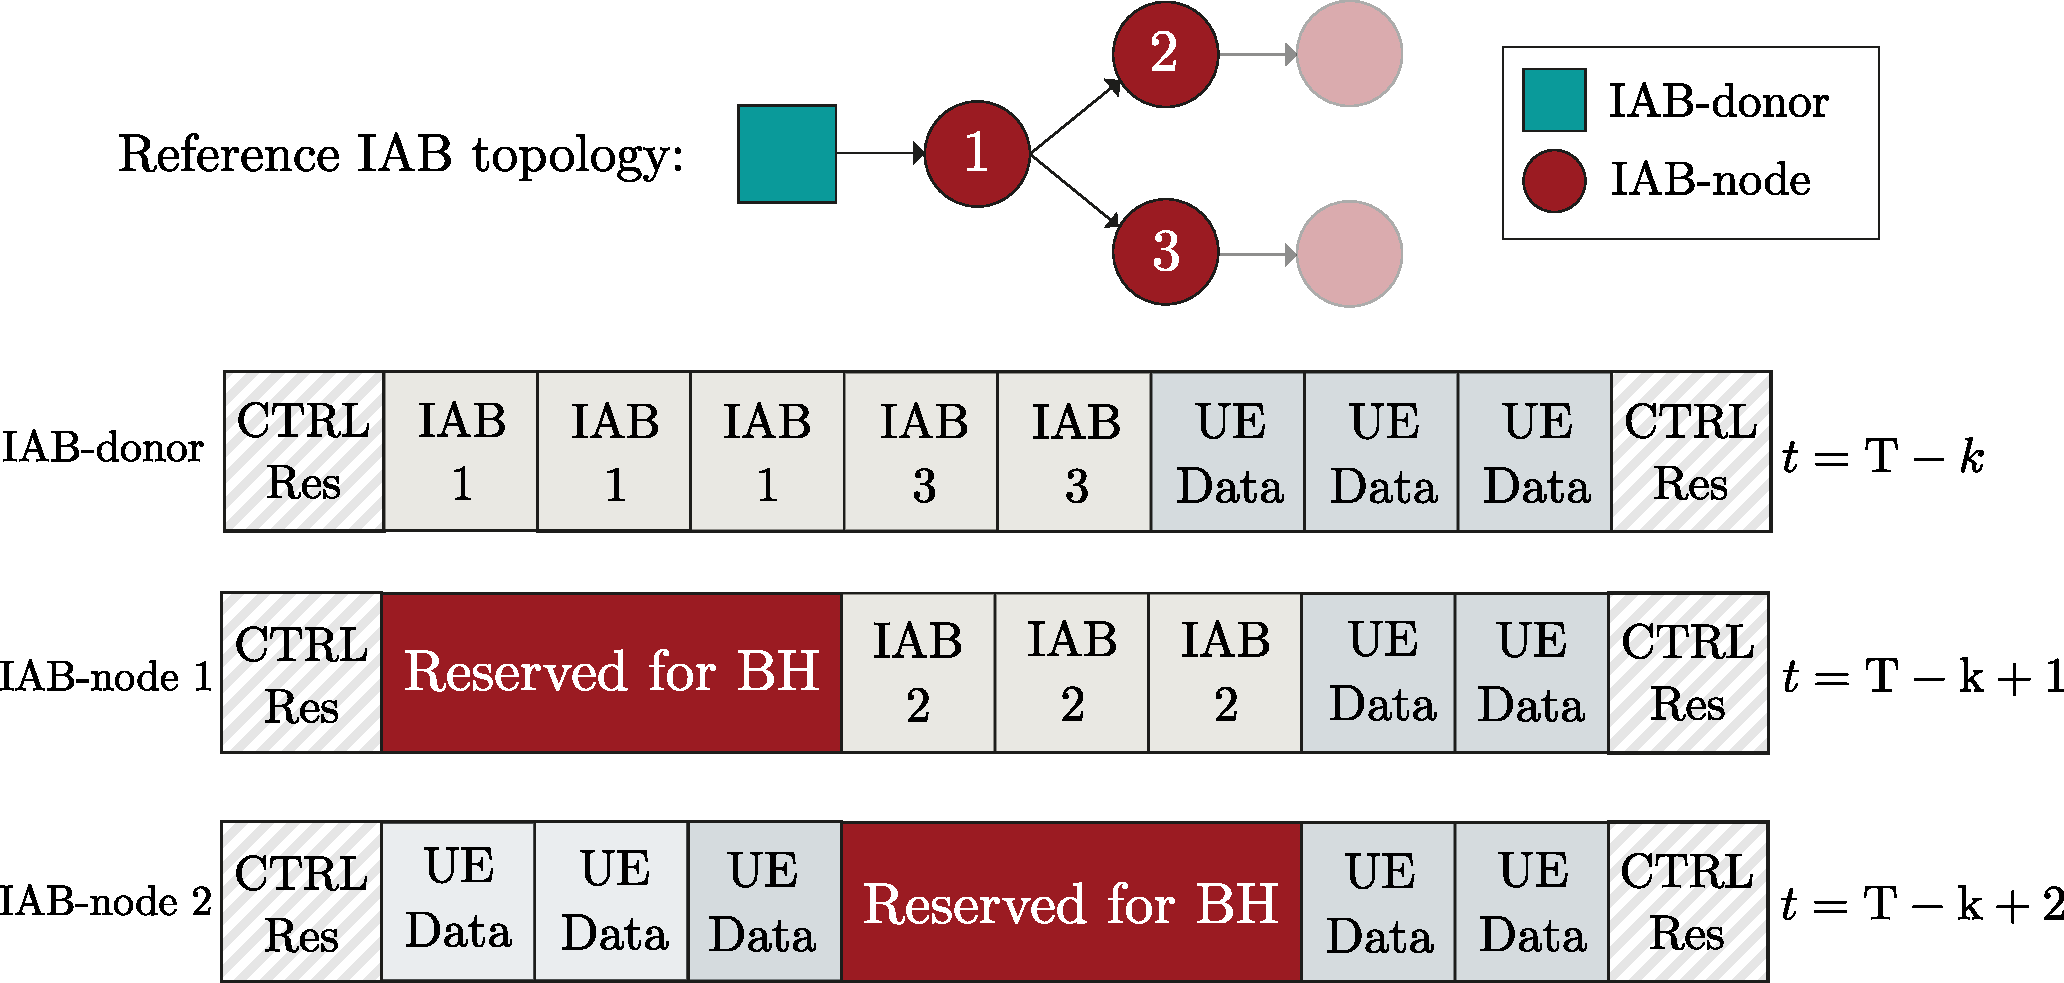
\includegraphics[width=0.75\linewidth]{IabSchedAlloc.pdf}
%\caption{Baseline distributed scheduler: example of a resource allocation at time $T$, for the depicted reference topology and where $k - 1$ indicates the maximum depth in the \gls{iab} network. Figure adapted from~\cite{polese2018end}.}
%\label{Fig:iab_sched_alloc}
%\vspace{-.6cm}
%\end{figure}

%An example of this scheduling mechanism is depicted in Fig.~\ref{Fig:iab_sched_alloc}: it can be noted how, for instance, the time resources which the donor has scheduled for backhauling purposes towards \gls{iab}-node 1 are marked as reserved by the latter. As a consequence, such node constraints its resource allocation to the remaining time slots only. 

\subsection{Simulation scenario and parameters}
The purpose of these simulations is to understand the performance of the proposed resource partitioning framework in the context of its target deployment, i.e., a multi-hop \gls{iab} network. As a consequence, the reference scenario consists of a dense urban deployment with a single \gls{iab}-donor and multiple \gls{iab}-nodes, as depicted in Fig.~\ref{Fig:Sim_scen}. In particular, the various \glspl{gnb} are distributed along an urban grid where the donor is located at the origin while the \gls{iab}-nodes are deployed along the street intersections, with a minimum inter-site distance of 100 m. The \gls{iab}-nodes attachments are computed using the so-called \textit{HQF} policy presented in~\cite{polese2018iab}; however, this choice does not introduce any loss of generality since such parameter is fixed for all the runs. A given number of \glspl{ue} are deployed within the surroundings of these base stations, with an initial position which is randomly sampled from circles of radius $\rho$ and whose centers are the various \glspl{gnb}. A summary of the simulation parameters in provided in Tab.~\ref{Tab:Sim_params}.
%Notably, the choice of not considering mobile \glspl{ue} is driven exclusively by concerns regarding the time needed to run our simulation campaigns. In fact, our framework introduces no limitations in such regard, due to the way the \gls{iab} topology is retrieved and the fact that we do not keep track of the per-flow information.
%The lack of mobility is mainly driven by concerns over the computational complexity of the simulations. 

\begin{figure}[tbp]
    \centering
    \subfloat[A realization of the simulation scenario; the dotted lines represent the cell-attachments of the \gls{iab}-nodes.\label{Fig:Sim_scen}]{
     % this sets the width of the figure, adjust to your needs
     \setlength\fwidth{0.7\columnwidth}
     % this sets the height of the figure, adjust to your needs
     \setlength\fheight{0.35\columnwidth}
       \raisebox{-.5\height}{\begin{tikzpicture}

    \definecolor{UNIPDRED}{RGB}{155,0,20}
	\definecolor{COMPLEMENTARY}{RGB}{0,153,153}
	\definecolor{DARKGREY}{RGB}{55,65,64}
	\definecolor{BLACK}{RGB}{20, 20, 20}
    
    \begin{axis}[
    width=\fwidth,
    height=\fheight,
    at={(0\fwidth,0\fheight)},
    scale only axis,
    legend style={
    	/tikz/every even column/.append style={column sep=0.3cm},
    	at={(0.5,0.98)},
    	anchor=south, 
    	draw=white!80!black, 
    	font=\small
    	},
    legend columns=3,
    %axis line style={white!80!black},
    %tick align=outside,
    %x grid style={white!80!black},
    xlabel style={font=\footnotesize},
    xlabel={},
    xtick={-100, -50, 0, 50, 100, 150},
    xmajorgrids,
    %xmajorticks=false,
    xmin=-150, xmax=150,
    xtick style={color=white!15!black},
    %y grid style={white!80!black},
    ylabel style={font=\footnotesize},
    ylabel={},
    ymajorgrids,
    %ymajorticks=false,
    ymin=-50, ymax=150,
    ytick style={color=white!15!black}
	]
	
	% IAB-node attachments
	\addplot[very thick, UNIPDRED, forget plot, dash pattern=on 5 pt off 3 pt] 
	table {%
	-100 0 
	0 0 
	};
	\addplot[very thick, UNIPDRED, forget plot, dash pattern=on 5 pt off 3 pt] 
	table {%
	100 100 
	0 0 
	};
	\addplot[very thick, UNIPDRED, forget plot, dash pattern=on 5 pt off 3 pt] 
	table {%
	-100 100 
	0 0 
	};
	\addplot[very thick, UNIPDRED, forget plot, dash pattern=on 5 pt off 3 pt] 
	table {%
	100 0 
	100 100 
	};
	\addplot[very thick, UNIPDRED, forget plot, dash pattern=on 5 pt off 3 pt] 
	table {%
	0 100 
	-100 100 
	};

    \addplot[
      scatter,
      only marks,
      scatter src=explicit,
      scatter/classes={1={DARKGREY, mark=square*}, 2={UNIPDRED, mark=diamond*}, 3={COMPLEMENTARY}},
      visualization depends on=\thisrow{sizedata}\as\sizedata,
      scatter/@pre marker code/.append style={
          /tikz/mark size=\sizedata
      }
    ]
    table[x=x,y=y, meta=class]{%
    x                      y                      sizedata                class
    0 0 5 1 
	100 0 6 2 
	-100 0 6 2 
	0 100 6 2 
	100 100 6 2 
	-100 100 6 2 
	28.8603 6.70813 2 3 
	22.1839 0.179283 2 3 
	-25.8695 -4.74675 2 3 
	-25.698 1.31045 2 3 
	-26.1185 5.61727 2 3 
	-18.8974 12.8042 2 3 
	-25.8278 8.77018 2 3 
	-11.9403 24.625 2 3 
	86.2329 -14.9938 2 3 
	113.411 -25.4381 2 3 
	80.796 10.6876 2 3 
	89.0457 9.21925 2 3 
	87.952 27.3012 2 3 
	89.4537 -0.761095 2 3 
	108.92 -15.5517 2 3 
	84.0229 -13.509 2 3 
	-71.3282 -2.49305 2 3 
	-114.738 26.7601 2 3 
	-115.867 28.3354 2 3 
	-117.757 24.2406 2 3 
	-103.439 -22.3846 2 3 
	-89.1148 5.80584 2 3 
	-116.494 -26.2217 2 3 
	-130.211 3.15653 2 3 
	-19.5929 85.0171 2 3 
	-22.2209 78.2847 2 3 
	13.0963 129.843 2 3 
	-15.409 112.165 2 3 
	-26.1002 118.747 2 3 
	12.3455 84.2945 2 3 
	-30.9925 96.9305 2 3 
	-33.7183 108.212 2 3 
	125.011 97.7272 2 3 
	112.293 126.281 2 3 
	113.959 76.0568 2 3 
	103.236 114.801 2 3 
	104.862 76.3655 2 3 
	131.206 109.996 2 3 
	114.825 128.336 2 3 
	90.7864 78.3714 2 3 
	-109.959 77.6437 2 3 
	-83.8184 115.384 2 3 
	-78.9347 82.8969 2 3 
	-114.208 81.4837 2 3 
	-123.238 80.8704 2 3 
	-104.259 88.5412 2 3 
	-94.1952 108.948 2 3 
	-114.781 80.0824 2 3 
    };
    \legend{\gls{iab}-donor, \gls{iab}-node, \gls{ue}}

    \end{axis}
    
\end{tikzpicture}




}
    }\hfill
    \subfloat[Simulation parameters.\label{Tab:Sim_params}]{
     \small
   \begin{tabular}{cc}
   \multicolumn{2}{c}{\textsc{Simulation parameters}}\\
   \hline
   \textsc{Parameter} & \textsc{Value} \\
   \hline
   Number of runs $N_{runs}$ & 25  \\
   \rowcolor{gray!15} Simulation time $T_{sim}$ & 3 s \\
   \gls{mwm} period $T_{alloc}$ & $\{ 1, 2, 4\}$ subframes \\
   \rowcolor{gray!15} Layer 4 protocol & $\{ $UDP, TCP$ \}$ \\
   UDP packet size $s_{UDP}$ & $\{50, 100, 200, 500 \}$ B \\
   \rowcolor{gray!15} Weight policy $f_u$ & $\{$\gls{msr}, \gls{ba}, \gls{mrba}$\}$ \\
   \hline
   \end{tabular}
    }
    \label{Float:Sim_scen_and_params}
    \caption{Simulation configuration.}
    \vspace{-.6cm}
\end{figure}

\section{Performance evaluation}
\label{Sec:perf_eval}

\begin{figure*}[tbp]
	\centering
	%\captionsetup{singlelinecheck=false, justification=justified}
  % this sets the width of the figure, adjust to your needs
  	\subfloat[$s_{UDP}$ = 100 B, i.e., \gls{udp} rate of 8 Mbps.\label{Fig:Thr_ECDF_100}]{
  	\setlength\fwidth{0.85\columnwidth}
    % this sets the height of the figure, adjust to your needs
    \setlength\fheight{0.33\columnwidth}
    % This file was created by tikzplotlib v0.9.4.
\begin{tikzpicture}

\pgfplotsset{every tick label/.append style={font=\footnotesize}}

\definecolor{UNIPDRED}{RGB}{155,0,20}
\definecolor{LIGHT_GREY}{RGB}{189,195,199}
\definecolor{COMPLEMENTARY}{RGB}{0,153,153}
\definecolor{DARKGREY}{RGB}{55,65,64}
\definecolor{SAND}{RGB}{180,160,135}

\begin{axis}[
width=\fwidth,
height=\fheight,
at={(0\fwidth,0\fheight)},
scale only axis,
%axis line style={white!80!black},
legend style={
    /tikz/every even column/.append style={column sep=0.2cm},
    at={(0.3,0.65)}, 
    anchor=south, 
    draw=white!80!black, 
    font=\scriptsize
    },
legend columns=2,
%tick align=outside,
%x grid style={white!80!black},
xlabel style={font=\footnotesize},
xlabel={UE throughput [Mbps]},
xtick={0, 1, 2, 3, 4, 5, 6, 7, 8},
xmajorgrids,
%xmajorticks=false,
xmin=0, xmax=8.5,
xtick style={color=white!15!black},
%y grid style={white!80!black},
ylabel shift = -1 pt,
ylabel style={font=\footnotesize},
ylabel={},
ymajorgrids,
%ymajorticks=false,
ymin=0, ymax=1.05,
ytick style={color=white!15!black},
ytick={0.2,0.4,0.6,0.8,1},
]

\addplot [very thick, SAND]
table {%
0.26964259147644 0
0.440404176712036 0.00265252590179443
0.609135508537292 0.00353670120239258
0.860332727432251 0.00442087650299072
1.0021516084671 0.00530505180358887
1.80407619476318 0.00618922710418701
1.86674773693085 0.00707340240478516
1.86872935295105 0.0079575777053833
1.86899101734161 0.00972592830657959
1.86937344074249 0.012378454208374
1.87010157108307 0.0159151554107666
1.87021577358246 0.0194518566131592
2.07712340354919 0.0203360319137573
2.41580104827881 0.0212202072143555
2.42250800132751 0.0229885578155518
2.49782967567444 0.0238727331161499
2.49792218208313 0.0300618410110474
2.49854469299316 0.0309460163116455
2.49861669540405 0.0362510681152344
2.53574633598328 0.0371352434158325
2.62055969238281 0.0380194187164307
2.62811470031738 0.0389035940170288
2.6283221244812 0.039787769317627
2.62947773933411 0.0406719446182251
2.62970066070557 0.0415561199188232
2.63152194023132 0.0424402952194214
2.63152813911438 0.0442086458206177
2.63292241096497 0.0450928211212158
2.70582509040833 0.045976996421814
2.7062041759491 0.0468611717224121
2.74750280380249 0.0477453470230103
2.74760341644287 0.052166223526001
2.74846625328064 0.0530503988265991
2.74853825569153 0.0557029247283936
2.75460028648376 0.0565871000289917
2.75477480888367 0.0592396259307861
2.7600576877594 0.0601238012313843
2.76282501220703 0.0610079765319824
2.76886248588562 0.0618921518325806
2.76891660690308 0.0654288530349731
2.77063202857971 0.0663130283355713
2.77686285972595 0.0671972036361694
2.77710485458374 0.0733864307403564
2.80236387252808 0.0742706060409546
2.8199348449707 0.0760389566421509
2.82017755508423 0.0822280645370483
2.85566520690918 0.0839964151382446
2.85595607757568 0.0901856422424316
2.8617091178894 0.0910698175430298
2.92173385620117 0.0919539928436279
2.92190027236938 0.0946065187454224
2.92191123962402 0.0963748693466187
2.92233276367188 0.0981432199478149
2.92234015464783 0.0999115705490112
2.92527842521667 0.100795745849609
2.92528581619263 0.101679921150208
2.9258246421814 0.102564096450806
2.929114818573 0.104332447052002
2.92912936210632 0.1052166223526
2.93662095069885 0.106100797653198
2.94025444984436 0.106984972953796
2.94139933586121 0.107869148254395
2.95004892349243 0.108753323554993
2.95006012916565 0.109637498855591
2.95263600349426 0.110521674156189
3.05221819877625 0.111405849456787
3.10105562210083 0.113174200057983
3.10163307189941 0.11494255065918
3.10173964500427 0.122015953063965
3.1021363735199 0.123784303665161
3.10239195823669 0.125552654266357
3.1034996509552 0.126436829566956
3.10382151603699 0.128205180168152
3.10409879684448 0.132626056671143
3.13609457015991 0.133510112762451
3.1746392250061 0.136162638664246
3.17652249336243 0.13881516456604
3.17669486999512 0.143236041069031
3.17720103263855 0.145004391670227
3.17746067047119 0.146772742271423
3.17749857902527 0.14854109287262
3.1819634437561 0.150309443473816
3.18213176727295 0.15296196937561
3.18215084075928 0.155614495277405
3.18521070480347 0.156498670578003
3.18546652793884 0.16268789768219
3.18967056274414 0.163572072982788
3.19050908088684 0.167108774185181
3.1905243396759 0.168877124786377
3.19163966178894 0.169761300086975
3.22586989402771 0.170645475387573
3.2259795665741 0.175950527191162
3.22825646400452 0.17683470249176
3.22887134552002 0.177718877792358
3.22895216941833 0.179487228393555
3.22963714599609 0.180371403694153
3.22964477539062 0.18213963508606
3.23387002944946 0.183023929595947
3.23403215408325 0.185676336288452
3.23405933380127 0.189213037490845
3.24865412712097 0.190097212791443
3.25200819969177 0.190981388092041
3.26675033569336 0.191865563392639
3.26687836647034 0.195402264595032
3.26724529266357 0.200707316398621
3.26732730865479 0.202475666999817
3.2810640335083 0.203359842300415
3.28848099708557 0.204244017601013
3.31646943092346 0.205128192901611
3.33002424240112 0.206012368202209
3.44054198265076 0.206896543502808
3.44539618492126 0.207780718803406
3.44547009468079 0.211317420005798
3.4528751373291 0.212201595306396
3.45287919044495 0.213085770606995
3.45335388183594 0.213969945907593
3.45357251167297 0.217506647109985
3.45441627502441 0.219274997711182
3.45453190803528 0.223695874214172
3.45682525634766 0.225464224815369
3.46599340438843 0.226348400115967
3.49390959739685 0.227232575416565
3.49476051330566 0.228116750717163
3.49514007568359 0.234305858612061
3.49550652503967 0.236074209213257
3.50014185905457 0.237842559814453
3.50015044212341 0.238726854324341
3.50125217437744 0.239610910415649
3.50149917602539 0.242263436317444
3.50174760818481 0.24403178691864
3.50176906585693 0.248452663421631
3.50679159164429 0.249336838722229
3.50679588317871 0.250221014022827
3.50864505767822 0.251105189323425
3.51900315284729 0.25375771522522
3.52100944519043 0.254641890525818
3.52105116844177 0.255526065826416
3.52260971069336 0.256410241127014
3.52292323112488 0.260831117630005
3.52386355400085 0.261715292930603
3.52944040298462 0.264367818832397
3.52968239784241 0.266136169433594
3.52969074249268 0.267020344734192
3.53243970870972 0.26790452003479
3.53249073028564 0.268788695335388
3.53440809249878 0.273209571838379
3.53442907333374 0.275862097740173
3.53707981109619 0.27763044834137
3.54024815559387 0.279398798942566
3.54046893119812 0.283819675445557
3.63516759872437 0.284703731536865
3.67046523094177 0.286472082138062
3.70479202270508 0.287356376647949
3.77303051948547 0.288240432739258
3.77917289733887 0.289124727249146
3.77976870536804 0.290893077850342
3.78155207633972 0.29177713394165
3.78209376335144 0.292661428451538
3.78363299369812 0.293545484542847
3.78388023376465 0.295313835144043
3.7852737903595 0.296198010444641
3.79006505012512 0.297082185745239
3.79036831855774 0.302387237548828
3.79567718505859 0.304155588150024
3.80048441886902 0.305039763450623
3.80264544487 0.305923938751221
3.80306959152222 0.308576464653015
3.80311512947083 0.309460639953613
3.82224583625793 0.310344815254211
3.8991870880127 0.31122899055481
3.90082430839539 0.312113165855408
3.90106749534607 0.313881516456604
3.90127801895142 0.317418217658997
3.90210723876953 0.318302392959595
3.90306997299194 0.323607444763184
3.9030978679657 0.327144145965576
3.92078280448914 0.328912496566772
3.92103576660156 0.331565022468567
3.92293262481689 0.332449197769165
3.92621231079102 0.333333373069763
3.98159027099609 0.334217548370361
3.98194789886475 0.340406656265259
3.98215365409851 0.341290950775146
4.01277494430542 0.342175006866455
4.01874113082886 0.343059301376343
4.0387282371521 0.343943357467651
4.05502891540527 0.345711708068848
4.16511964797974 0.346596002578735
4.17559957504272 0.347480058670044
4.23066568374634 0.348364353179932
4.24002552032471 0.350132584571838
4.27321434020996 0.351016759872437
4.2744312286377 0.352785110473633
4.27443647384644 0.353669285774231
4.30599355697632 0.354553461074829
4.3209490776062 0.355437636375427
4.3435754776001 0.356321811676025
4.58782386779785 0.358090162277222
4.64074563980103 0.359858512878418
4.64150619506836 0.362511038780212
4.64165592193604 0.363395214080811
4.64242935180664 0.365163564682007
4.64243507385254 0.366047739982605
4.72712326049805 0.366931915283203
4.72848701477051 0.371352791786194
4.72852659225464 0.37312114238739
4.73176956176758 0.374005317687988
4.73201608657837 0.374889492988586
4.73816013336182 0.375773668289185
4.99486064910889 0.376657843589783
4.99780225753784 0.377542018890381
4.9992036819458 0.378426194190979
4.99922752380371 0.379310369491577
5.00031185150146 0.380194544792175
5.00619983673096 0.381078720092773
5.00699758529663 0.38284707069397
5.00713300704956 0.386383771896362
5.00887537002563 0.389036178588867
5.00924777984619 0.39257287979126
5.0092716217041 0.393457174301147
5.01016283035278 0.396109580993652
5.36077451705933 0.397877931594849
5.45640563964844 0.398762226104736
5.59347248077393 0.399646282196045
5.59372854232788 0.404951333999634
5.71079158782959 0.405835509300232
5.71807241439819 0.40671968460083
5.71811294555664 0.407603859901428
5.71947479248047 0.408488035202026
5.71977233886719 0.409372210502625
5.9135046005249 0.410256385803223
5.95501756668091 0.411140561103821
5.96454858779907 0.412024736404419
5.96482753753662 0.413793087005615
5.96508502960205 0.41644561290741
5.98064374923706 0.417329788208008
6.34759044647217 0.418213963508606
6.48497629165649 0.419982314109802
6.4860372543335 0.4208664894104
6.48632860183716 0.425287365913391
6.48778867721558 0.426171541213989
6.50417757034302 0.427055716514587
6.50450038909912 0.428824067115784
6.504554271698 0.432360768318176
6.53208923339844 0.433244943618774
6.53364706039429 0.435013294219971
6.53366279602051 0.435897469520569
6.71247386932373 0.437665820121765
6.71300649642944 0.438549995422363
6.85143709182739 0.439434170722961
6.85148572921753 0.44031834602356
6.85364723205566 0.441202402114868
6.85380268096924 0.442970752716064
6.87466621398926 0.443855047225952
6.95184946060181 0.444739103317261
6.96869039535522 0.446507453918457
6.96899509429932 0.450928449630737
6.97008609771729 0.451812505722046
7.01210975646973 0.452696800231934
7.01526260375977 0.453580856323242
7.02312421798706 0.45446503162384
7.02828359603882 0.456233382225037
7.02868795394897 0.458885908126831
7.03365659713745 0.459770083427429
7.03687238693237 0.461538434028625
7.03884840011597 0.463306784629822
7.03897762298584 0.465075135231018
7.04769659042358 0.467727661132812
7.04871797561646 0.470380187034607
7.04896020889282 0.476569414138794
7.06435680389404 0.477453589439392
7.06582593917847 0.47833776473999
7.06814908981323 0.479221940040588
7.06824493408203 0.480106115341187
7.07024717330933 0.480990290641785
7.07034254074097 0.483642816543579
7.10552263259888 0.484526991844177
7.10553121566772 0.485411167144775
7.12034606933594 0.486295342445374
7.12035465240479 0.487179517745972
7.12568378448486 0.48806369304657
7.12577247619629 0.488947868347168
7.12878942489624 0.491600394248962
7.12909984588623 0.494252920150757
7.12917041778564 0.496905326843262
7.19264221191406 0.498673677444458
7.19721364974976 0.499557971954346
7.19817972183228 0.500442028045654
7.19826078414917 0.504863023757935
7.20064449310303 0.505747079849243
7.20089721679688 0.507515430450439
7.20201778411865 0.508399724960327
7.20212602615356 0.512820482254028
7.20610332489014 0.513704657554626
7.27363061904907 0.514588832855225
7.27442312240601 0.515473008155823
7.27444124221802 0.517241358757019
7.2751145362854 0.518125534057617
7.27545595169067 0.520778059959412
7.27801990509033 0.52166223526001
7.27887773513794 0.522546410560608
7.2790994644165 0.528735637664795
7.28205442428589 0.529619812965393
7.28302431106567 0.530503988265991
7.28306102752686 0.531388163566589
7.36370086669922 0.532272338867188
7.36590242385864 0.533156514167786
7.42193555831909 0.534924864768982
7.42232847213745 0.537577390670776
7.54834079742432 0.538461565971375
7.54871797561646 0.540229797363281
7.54880714416504 0.544650793075562
7.68753862380981 0.54553484916687
7.75189876556396 0.547303199768066
7.7585825920105 0.548187494277954
7.7586555480957 0.554376602172852
7.78432655334473 0.555260896682739
7.78829669952393 0.556144952774048
7.78843402862549 0.55968165397644
7.80472946166992 0.560565948486328
7.80569553375244 0.562334299087524
7.805748462677 0.566755056381226
7.84723281860352 0.567639231681824
7.84967947006226 0.571175932884216
7.84972238540649 0.573828458786011
7.88307237625122 0.574712634086609
7.88419818878174 0.575596809387207
7.88420915603638 0.576480984687805
7.88542222976685 0.5791335105896
7.88546514511108 0.580901861190796
7.90265941619873 0.581786036491394
7.93057441711426 0.582670211791992
7.93491506576538 0.58355438709259
7.93495893478394 0.587091088294983
7.93593549728394 0.587975263595581
7.93594646453857 0.588859438896179
7.94893455505371 0.589743614196777
7.9490761756897 0.590627789497375
7.94977140426636 0.591511964797974
7.95147800445557 0.592396020889282
7.95183038711548 0.59328031539917
7.9531192779541 0.594164371490479
7.95380258560181 0.596817016601562
7.9541220664978 0.599469423294067
7.95531272888184 0.600353717803955
7.95600700378418 0.602122068405151
7.95806932449341 0.60300612449646
7.95811367034912 0.603890419006348
7.95934963226318 0.604774475097656
7.95951461791992 0.606542825698853
7.9607720375061 0.60742712020874
7.96089458465576 0.608311176300049
7.96199893951416 0.609195470809937
7.96215343475342 0.615384578704834
7.96322441101074 0.616268873214722
7.9634895324707 0.622457981109619
7.96455001831055 0.623342156410217
7.96477127075195 0.627763032913208
7.96508073806763 0.629531383514404
7.96534585952759 0.633952260017395
7.96560001373291 0.635720610618591
7.96586561203003 0.640141487121582
7.96607542037964 0.641909837722778
7.9674243927002 0.780725002288818
7.96773386001587 0.887709975242615
7.96797704696655 0.889478325843811
7.96834135055542 0.897435903549194
7.96849679946899 0.900972604751587
7.96870708465576 0.946065425872803
7.96904993057251 0.999115824699402
8.5 1
};
\addlegendentry{Distr}


\addplot [very thick, COMPLEMENTARY, mark=square*, mark repeat=60, mark phase=40]
table {%
0.000693440437316895 0
0.119515538215637 0.000922560691833496
0.159256935119629 0.00184500217437744
0.597056031227112 0.00461256504058838
0.712712645530701 0.00553500652313232
0.726806163787842 0.00645756721496582
0.726821184158325 0.0119925737380981
0.759883642196655 0.0129151344299316
0.760014295578003 0.0193727016448975
0.992992997169495 0.0202951431274414
1.00686490535736 0.0212177038192749
1.00782418251038 0.0221402645111084
1.0082551240921 0.0276752710342407
1.07422256469727 0.0285978317260742
1.23650026321411 0.0295202732086182
1.24447298049927 0.0304428339004517
1.24472653865814 0.0341328382492065
1.25939452648163 0.03505539894104
1.26051843166351 0.035977840423584
1.3560699224472 0.0369004011154175
1.37027359008789 0.0387454032897949
1.37027680873871 0.0396678447723389
1.37143182754517 0.0405904054641724
1.37257981300354 0.0424354076385498
1.3732488155365 0.0433579683303833
1.44303858280182 0.0442804098129272
1.44760024547577 0.0452029705047607
1.44767200946808 0.0553505420684814
1.44881331920624 0.0562731027603149
1.44886040687561 0.0581181049346924
1.4539886713028 0.0599631071090698
1.45400047302246 0.0636531114578247
1.46569454669952 0.0645756721496582
1.5681084394455 0.0654981136322021
1.56836795806885 0.0673432350158691
1.56838297843933 0.071955680847168
1.9457221031189 0.0728782415390015
1.94600713253021 0.0747232437133789
1.946009516716 0.0756458044052124
1.94791996479034 0.0765682458877563
1.9479501247406 0.0784132480621338
1.95214557647705 0.0793358087539673
1.95215487480164 0.0830258131027222
1.95394539833069 0.0839483737945557
1.95394778251648 0.0848708152770996
1.99196577072144 0.0857933759689331
2.00361347198486 0.0867158174514771
2.02677488327026 0.0876383781433105
2.03139662742615 0.088560938835144
2.03273844718933 0.089483380317688
2.03275299072266 0.0913283824920654
2.03436756134033 0.0922509431838989
2.11717700958252 0.0931733846664429
2.12111163139343 0.0940959453582764
2.12173199653625 0.0959409475326538
2.12183690071106 0.104243516921997
2.12198424339294 0.106088519096375
2.12270855903625 0.107011079788208
2.12271428108215 0.108856081962585
2.1304190158844 0.109778642654419
2.13463735580444 0.110701084136963
2.13466668128967 0.113468647003174
2.13652753829956 0.114391088485718
2.18809390068054 0.116236209869385
2.1887571811676 0.117158651351929
2.18899250030518 0.122693777084351
2.21482110023499 0.123616218566895
2.21729159355164 0.125461220741272
2.22486162185669 0.126383781433105
2.22808194160461 0.127306222915649
2.22856187820435 0.128228783607483
2.23040413856506 0.129151344299316
2.26028728485107 0.13007378578186
2.26797556877136 0.130996346473694
2.26861238479614 0.136531352996826
2.27123975753784 0.13745391368866
2.36648774147034 0.138376355171204
2.36989164352417 0.139298915863037
2.37159609794617 0.140221357345581
2.37233400344849 0.142988920211792
2.37260818481445 0.143911480903625
2.41940212249756 0.144833922386169
2.41964530944824 0.145756483078003
2.42206501960754 0.146678924560547
2.42693829536438 0.14760148525238
2.42717909812927 0.151291489601135
2.4275426864624 0.152214050292969
2.42995262145996 0.153136491775513
2.43535137176514 0.154059052467346
2.43768572807312 0.15498161315918
2.44726800918579 0.155904054641724
2.46195650100708 0.156826615333557
2.46219205856323 0.160516619682312
2.46288466453552 0.161439180374146
2.46297359466553 0.163284182548523
2.46382284164429 0.164206624031067
2.47657942771912 0.1651291847229
2.47667551040649 0.166051626205444
2.47775530815125 0.166974186897278
2.47780537605286 0.169741630554199
2.49199962615967 0.170664191246033
2.4981062412262 0.171586751937866
2.49834179878235 0.174354195594788
2.49867010116577 0.176199197769165
2.49881720542908 0.178966760635376
2.4992470741272 0.180811762809753
2.49961495399475 0.184501886367798
2.50682592391968 0.185424327850342
2.50773572921753 0.187269330024719
2.50836801528931 0.188191890716553
2.50860404968262 0.196494460105896
2.50996613502502 0.197417020797729
2.51020765304565 0.199262022972107
2.52322888374329 0.202952027320862
2.52448034286499 0.204797029495239
2.52550864219666 0.205719590187073
2.52551198005676 0.206642031669617
2.52628231048584 0.20756459236145
2.53637742996216 0.208487033843994
2.53685307502747 0.209409594535828
2.53725171089172 0.215867161750793
2.53755116462708 0.217712163925171
2.5375611782074 0.220479726791382
2.54133033752441 0.221402168273926
2.54211711883545 0.223247289657593
2.54214453697205 0.22509229183197
2.54261207580566 0.226014733314514
2.55435681343079 0.226937294006348
2.55480432510376 0.227859735488892
2.55734658241272 0.228782296180725
2.57158017158508 0.230627298355103
2.57307934761047 0.231549859046936
2.58276295661926 0.234317302703857
2.58307123184204 0.235239863395691
2.584144115448 0.236162424087524
2.59009289741516 0.238929867744446
2.60104560852051 0.240774869918823
2.6070122718811 0.241697430610657
2.61967539787292 0.24261999130249
2.66720509529114 0.244464993476868
2.66725587844849 0.245387434959412
2.72790575027466 0.247232437133789
2.72818279266357 0.251845002174377
2.72862124443054 0.252767562866211
2.73049545288086 0.253690004348755
2.73609709739685 0.255535125732422
2.736483335495 0.259225130081177
2.73679137229919 0.261992692947388
2.81280612945557 0.263837575912476
2.83584880828857 0.264760136604309
2.83783507347107 0.265682697296143
2.95929646492004 0.269372701644897
2.96097469329834 0.270295143127441
2.96567916870117 0.271217703819275
2.96619153022766 0.272140264511108
2.96729707717896 0.273062705993652
2.96801328659058 0.27490770816803
2.96865940093994 0.275830268859863
2.96866989135742 0.276752710342407
2.97192597389221 0.277675271034241
2.97657895088196 0.280442833900452
2.99721527099609 0.282287836074829
3.0449481010437 0.284132838249207
3.04524064064026 0.290590405464172
3.05891418457031 0.291512966156006
3.05913615226746 0.29243540763855
3.09333443641663 0.293357968330383
3.10531139373779 0.295202970504761
3.16781735420227 0.296125411987305
3.18863844871521 0.297047972679138
3.18915510177612 0.297970533370972
3.18941736221313 0.303505539894104
3.18967962265015 0.305350542068481
3.18969559669495 0.309040546417236
3.19570779800415 0.30996310710907
3.19670009613037 0.310885667800903
3.19858813285828 0.311808109283447
3.2024610042572 0.312730669975281
3.20366549491882 0.313653111457825
3.20367336273193 0.314575672149658
3.20530080795288 0.315498113632202
3.20531678199768 0.316420674324036
3.36194229125977 0.317343235015869
3.42266368865967 0.318265676498413
3.42354035377502 0.320110678672791
3.42375755310059 0.324723243713379
3.50149536132812 0.325645685195923
3.51525497436523 0.326568245887756
3.56066226959229 0.328413248062134
3.56259059906006 0.330258369445801
3.5631160736084 0.331180810928345
3.56805229187012 0.332103252410889
3.568204164505 0.333948373794556
3.5710117816925 0.3348708152771
3.57147884368896 0.336715936660767
3.58437633514404 0.337638378143311
3.58603763580322 0.338560819625854
3.58673048019409 0.340405941009521
3.58921003341675 0.342250943183899
3.60637378692627 0.343173503875732
3.61262488365173 0.344095945358276
3.62165451049805 0.34501838684082
3.6219437122345 0.349630951881409
3.62346935272217 0.350553512573242
3.6261613368988 0.351475954055786
3.62666988372803 0.35239851474762
3.63200402259827 0.354243516921997
3.63224840164185 0.356088519096375
3.63386368751526 0.357011079788208
3.68670630455017 0.357933521270752
3.69633603096008 0.358856081962585
3.69879579544067 0.359778642654419
3.72128319740295 0.360701084136963
3.72143459320068 0.361623644828796
3.74851179122925 0.36254608631134
3.75784826278687 0.363468647003174
3.75816464424133 0.365313649177551
3.75844478607178 0.369003653526306
3.7591495513916 0.36992621421814
3.75941681861877 0.374538779258728
3.76022744178772 0.375461220741272
3.79992628097534 0.376383781433105
3.80160331726074 0.377306222915649
3.85554623603821 0.38007378578186
3.876544713974 0.380996346473694
3.94954562187195 0.381918787956238
4.02695846557617 0.383763790130615
4.09507656097412 0.384686350822449
4.12194061279297 0.386531352996826
4.14429044723511 0.38745391368866
4.35945320129395 0.390221357345581
4.35966157913208 0.392066478729248
4.36110973358154 0.392988920211792
4.36112546920776 0.393911480903625
4.39790821075439 0.395756483078003
4.4080286026001 0.396678924560547
4.41130590438843 0.39760148525238
4.87467813491821 0.398524045944214
4.9422812461853 0.399446487426758
4.95907831192017 0.400369048118591
4.96778535842896 0.402214050292969
4.97122573852539 0.403136491775513
4.97210836410522 0.404059052467346
4.97302675247192 0.407749056816101
4.98327779769897 0.408671617507935
5.00254821777344 0.409594058990479
5.00930595397949 0.410516619682312
5.0093297958374 0.412361621856689
5.01085090637207 0.413284063339233
5.04663467407227 0.414206624031067
5.13907670974731 0.4151291847229
5.34705781936646 0.416051626205444
5.34793853759766 0.416974186897278
5.35226726531982 0.417896747589111
5.38592481613159 0.418819189071655
5.38914728164673 0.419741630554199
5.39950656890869 0.420664191246033
5.42634010314941 0.421586751937866
5.45551300048828 0.423431754112244
5.55426406860352 0.424354314804077
5.55430364608765 0.427121758460999
5.63289642333984 0.428044319152832
6.02040863037109 0.430811882019043
6.02500772476196 0.431734323501587
6.08387899398804 0.432656764984131
6.73705244064331 0.433579325675964
6.74483633041382 0.434501886367798
6.74887037277222 0.435424327850342
6.7491021156311 0.439114332199097
6.85364723205566 0.440959453582764
6.85635662078857 0.441881895065308
6.87699699401855 0.444649457931519
6.87701320648193 0.445571899414062
6.87871122360229 0.446494460105896
6.8796010017395 0.447417020797729
6.88149785995483 0.448339462280273
6.88155555725098 0.450184464454651
6.88558340072632 0.451107025146484
6.88758230209351 0.452029466629028
6.89099740982056 0.452952027320862
6.89266014099121 0.453874588012695
6.89994239807129 0.454797029495239
6.90160942077637 0.456642031669617
6.91130590438843 0.45756459236145
6.9207124710083 0.459409594535828
6.92298269271851 0.461254596710205
6.9279203414917 0.462177157402039
6.95650482177734 0.463099598884583
6.95882415771484 0.464022159576416
6.97282075881958 0.46494460105896
6.98741865158081 0.466789722442627
6.98815011978149 0.467712163925171
7.00506782531738 0.468634724617004
7.00670099258423 0.469557166099548
7.00720548629761 0.472324728965759
7.00770139694214 0.473247289657593
7.00770998001099 0.474169731140137
7.00936126708984 0.47509229183197
7.01292324066162 0.476014733314514
7.0336480140686 0.477859735488892
7.05020666122437 0.478782296180725
7.05145359039307 0.479704856872559
7.06788778305054 0.480627298355103
7.07065629959106 0.481549859046936
7.07211971282959 0.48247230052948
7.08277320861816 0.483394861221313
7.08382177352905 0.484317302703857
7.08559703826904 0.485239863395691
7.08585929870605 0.486162424087524
7.08767032623291 0.487084865570068
7.08778381347656 0.488007307052612
7.09101438522339 0.489852428436279
7.0950984954834 0.490774869918823
7.09628248214722 0.491697430610657
7.09643125534058 0.494464874267578
7.09959077835083 0.497232437133789
7.10164594650269 0.498154997825623
7.10471343994141 0.499077558517456
7.10477495193481 0.5
7.12326955795288 0.500922441482544
7.1237211227417 0.501845002174377
7.12589645385742 0.502767562866211
7.1291880607605 0.503690004348755
7.13091468811035 0.505535125732422
7.13128709793091 0.506457567214966
7.13555908203125 0.50738000869751
7.13758230209351 0.508302569389343
7.13759994506836 0.510147571563721
7.1408314704895 0.511070132255554
7.1425461769104 0.513837575912476
7.16809701919556 0.514760136604309
7.17349863052368 0.515682697296143
7.17351627349854 0.516605138778687
7.19400310516357 0.518450260162354
7.19401216506958 0.519372701644897
7.20268630981445 0.520295143127441
7.20301151275635 0.522140264511108
7.21727418899536 0.523062705993652
7.21957015991211 0.523985266685486
7.21958827972412 0.525830268859863
7.31250619888306 0.526752710342407
7.31355905532837 0.527675271034241
7.31362438201904 0.528597831726074
7.31456565856934 0.529520273208618
7.3147144317627 0.533210277557373
7.37175703048706 0.534132838249207
7.37609481811523 0.53505539894104
7.3762845993042 0.537822961807251
7.37632274627686 0.540590405464172
7.55123043060303 0.541512966156006
7.55334615707397 0.54243540763855
7.58306884765625 0.543357849121094
7.5868067741394 0.544280529022217
7.59393215179443 0.545202970504761
7.59402275085449 0.547970533370972
7.61951303482056 0.548892974853516
7.62096929550171 0.54981541633606
7.62558555603027 0.550738096237183
7.62667989730835 0.551660537719727
7.62693309783936 0.555350542068481
7.68902111053467 0.556272983551025
7.72382164001465 0.557195544242859
7.74306344985962 0.558118104934692
7.74579000473022 0.559040546417236
7.75875043869019 0.55996310710907
7.76130962371826 0.560885667800903
7.76247453689575 0.561808109283447
7.76265287399292 0.563653111457825
7.79379463195801 0.564575672149658
7.79404878616333 0.565498113632202
7.79484272003174 0.566420674324036
7.79517078399658 0.571033239364624
7.8927321434021 0.571955680847168
7.9016695022583 0.572878241539001
7.90321445465088 0.579335808753967
7.93168115615845 0.582103252410889
7.95135688781738 0.583025813102722
7.95372581481934 0.583948373794556
7.95413303375244 0.586715936660767
7.95533466339111 0.588560819625854
7.95557737350464 0.590405941009521
7.95690059661865 0.591328382492065
7.95977973937988 0.596863508224487
7.96177816390991 0.598708510398865
7.96199893951416 0.601475954055786
7.96295928955078 0.60239851474762
7.9632134437561 0.604243516921997
7.9634895324707 0.608856081962585
7.96401882171631 0.609778642654419
7.96428489685059 0.611623644828796
7.96455001831055 0.613468647003174
7.96551084518433 0.630996227264404
7.9656777381897 0.633763790130615
7.96746826171875 0.816420674324036
7.96772289276123 0.867158651351929
7.96796607971191 0.869003772735596
7.96837425231934 0.876383781433105
7.96856355667114 0.879151344299316
7.96865224838257 0.917896747589111
7.96897268295288 0.999077558517456
8.5 1
};
\addlegendentry{\gls{msr}}

\addplot [very thick, DARKGREY, mark=*, mark repeat=60, mark phase=40]
table {%
0.234191179275513 0
0.281193256378174 0.00118064880371094
0.577000975608826 0.00236129760742188
0.63570237159729 0.00354194641113281
0.715597152709961 0.00472259521484375
2.6375572681427 0.00826442241668701
2.79069304466248 0.00944507122039795
2.88134479522705 0.0106257200241089
3.13204503059387 0.0118063688278198
3.14603781700134 0.0129870176315308
3.27042412757874 0.0141676664352417
3.65718984603882 0.0165289640426636
3.66828012466431 0.0177096128463745
3.85161876678467 0.0188901424407959
4.45079612731934 0.0212514400482178
4.52173185348511 0.0224320888519287
4.81968212127686 0.0236127376556396
5.00756978988647 0.0247933864593506
5.12364816665649 0.0259740352630615
5.47601079940796 0.0271546840667725
5.55078983306885 0.0283353328704834
5.80145311355591 0.0306966304779053
5.80315160751343 0.0318771600723267
5.80337381362915 0.0389610528945923
5.82239866256714 0.0401417016983032
5.82262086868286 0.0460448265075684
5.8230938911438 0.0472254753112793
6.00642681121826 0.0484061241149902
6.12701177597046 0.0495867729187012
6.17299699783325 0.0507674217224121
6.17315292358398 0.053128719329834
6.17396926879883 0.0543093681335449
6.17413330078125 0.0590318441390991
6.19868755340576 0.0602124929428101
6.19936847686768 0.061393141746521
6.20334625244141 0.0625737905502319
6.20465517044067 0.0637544393539429
6.20956516265869 0.0649350881576538
6.20965385437012 0.0672963857650757
6.22274255752563 0.0684769153594971
6.22341108322144 0.0708382129669189
6.22371101379395 0.0767414569854736
6.2290415763855 0.0779221057891846
6.23125219345093 0.0791027545928955
6.23155546188354 0.0861865282058716
6.2318000793457 0.0885478258132935
6.23534774780273 0.0897284746170044
6.23544311523438 0.0968122482299805
6.24525499343872 0.0979928970336914
6.24762630462646 0.0991735458374023
6.24795055389404 0.109799265861511
6.24859094619751 0.110979914665222
6.24881458282471 0.114521861076355
6.24885940551758 0.115702509880066
6.30343389511108 0.116883158683777
6.49414300918579 0.118063807487488
6.49481868743896 0.123966932296753
6.4948263168335 0.125147581100464
6.49542331695557 0.126328229904175
6.49547004699707 0.133412003517151
6.49991273880005 0.134592652320862
6.50055313110352 0.135773301124573
6.50082921981812 0.142857193946838
6.50360870361328 0.14403772354126
6.50397443771362 0.152302265167236
6.50939321517944 0.153482913970947
6.51118469238281 0.154663562774658
6.51146125793457 0.160566687583923
6.51471042633057 0.161747336387634
6.51506376266479 0.170011758804321
6.54694223403931 0.171192407608032
6.54775238037109 0.172373056411743
6.54802846908569 0.179456949234009
6.54883432388306 0.18063759803772
6.54892778396606 0.186540722846985
6.60878324508667 0.187721371650696
6.61003971099854 0.188902020454407
6.61057043075562 0.190082669258118
6.61864233016968 0.191263318061829
6.62090349197388 0.19244396686554
6.62114858627319 0.193624496459961
6.62281608581543 0.194805145263672
6.62286376953125 0.197166442871094
6.62870597839355 0.198347091674805
6.63044548034668 0.200708389282227
6.63075733184814 0.203069686889648
6.63173198699951 0.204250335693359
6.63178730010986 0.210153460502625
6.63322639465332 0.211334109306335
6.63388299942017 0.21723735332489
6.63473892211914 0.218417882919312
6.63480234146118 0.221959829330444
6.63534879684448 0.223140478134155
6.6353645324707 0.224321126937866
6.64044427871704 0.225501775741577
6.65826416015625 0.226682424545288
6.65831184387207 0.227863073348999
6.65894508361816 0.22904372215271
6.66067028045654 0.230224370956421
6.66130256652832 0.231405019760132
6.66305732727051 0.232585549354553
6.6633939743042 0.247933864593506
6.66427230834961 0.249114513397217
6.66447782516479 0.25265645980835
6.66450977325439 0.256198406219482
6.66619348526001 0.257379055023193
6.66637659072876 0.264462828636169
6.70076084136963 0.26564347743988
6.72005796432495 0.266824126243591
6.72196578979492 0.268004655838013
6.72199821472168 0.271546602249146
6.7226676940918 0.272727251052856
6.72272443771362 0.280991792678833
6.76421022415161 0.282172441482544
6.76430892944336 0.284533619880676
6.78140926361084 0.285714268684387
6.7816948890686 0.293978691101074
6.79471206665039 0.295159339904785
6.79652547836304 0.296339988708496
6.79733276367188 0.298701286315918
6.79770708084106 0.303423881530762
6.79794073104858 0.305785179138184
6.79798984527588 0.310507655143738
6.83917284011841 0.311688303947449
6.83949947357178 0.316410899162292
6.84021949768066 0.317591428756714
6.84061241149902 0.32585597038269
6.84079122543335 0.334120392799377
6.84119987487793 0.343565464019775
6.84451484680176 0.344746112823486
6.84469509124756 0.348288059234619
6.84473609924316 0.353010654449463
6.85029602050781 0.354191303253174
6.86941242218018 0.355371952056885
6.86956882476807 0.356552600860596
6.87249898910522 0.357733249664307
6.87255001068115 0.358913779258728
6.87306118011475 0.360094428062439
6.8731632232666 0.362455725669861
6.94546318054199 0.363636374473572
6.98510313034058 0.364817023277283
6.98515558242798 0.365997672080994
7.0257716178894 0.367178320884705
7.03333759307861 0.368358850479126
7.03713989257812 0.369539499282837
7.08486223220825 0.370720148086548
7.10189533233643 0.371900796890259
7.10194969177246 0.37308144569397
7.11906576156616 0.374262094497681
7.11914491653442 0.382526636123657
7.1237211227417 0.383707165718079
7.12441921234131 0.3860684633255
7.12495851516724 0.387249112129211
7.12517070770264 0.389610409736633
7.1262059211731 0.393152236938477
7.12664794921875 0.403778076171875
7.1276216506958 0.407320022583008
7.12770986557007 0.412042498588562
7.13669490814209 0.413223147392273
7.13941955566406 0.414403796195984
7.13985443115234 0.422668218612671
7.14984941482544 0.423848867416382
7.15009880065918 0.430932760238647
7.15110540390015 0.432113409042358
7.15116739273071 0.439197182655334
7.15798854827881 0.440377831459045
7.15889930725098 0.441558480262756
7.16438674926758 0.443919658660889
7.16461753845215 0.446280956268311
7.16466188430786 0.451003551483154
7.17371368408203 0.452184200286865
7.17488813400269 0.453364849090576
7.17522001266479 0.459267973899841
7.17820739746094 0.460448622703552
7.18009281158447 0.461629271507263
7.18014669418335 0.468713045120239
7.20384311676025 0.46989369392395
7.20500040054321 0.471074342727661
7.23035955429077 0.472254991531372
7.24466133117676 0.473435640335083
7.33897113800049 0.474616289138794
7.34754705429077 0.475796937942505
7.39095687866211 0.476977586746216
7.45756053924561 0.478158235549927
7.46381425857544 0.479338884353638
7.47392988204956 0.480519533157349
7.50526571273804 0.48170018196106
7.50832843780518 0.485242009162903
7.50846576690674 0.499409675598145
7.52174139022827 0.501770973205566
7.52270269393921 0.502951622009277
7.52311658859253 0.505312919616699
7.52316617965698 0.510035395622253
7.60781002044678 0.511216044425964
7.61590433120728 0.512396693229675
7.61735963821411 0.513577342033386
7.6306939125061 0.514757990837097
7.69751691818237 0.51829981803894
7.69755792617798 0.519480466842651
7.71661996841431 0.520661115646362
7.71698999404907 0.521841764450073
7.72263765335083 0.523022413253784
7.78663778305054 0.524203062057495
7.86779594421387 0.526564359664917
7.86843204498291 0.527745008468628
7.87892866134644 0.528925657272339
7.88024806976318 0.53010630607605
7.8803129196167 0.536009430885315
7.88176298141479 0.537190079689026
7.88681936264038 0.538370728492737
7.88808727264404 0.539551377296448
7.90061473846436 0.540731906890869
7.90190887451172 0.543093204498291
7.9021372795105 0.546635150909424
7.90217018127441 0.548996448516846
7.90732622146606 0.550177097320557
7.90760135650635 0.552538394927979
7.90763425827026 0.556080341339111
7.90927934646606 0.557260990142822
7.909508228302 0.561983466148376
7.91154670715332 0.563164114952087
7.92654466629028 0.564344763755798
7.92678546905518 0.566705942153931
7.92703723907471 0.569067239761353
7.92784738540649 0.573789834976196
7.92806625366211 0.574970483779907
7.93442153930664 0.577331781387329
7.93443250656128 0.57851243019104
7.93546342849731 0.579693078994751
7.93574857711792 0.587957501411438
7.93662691116333 0.589138150215149
7.9372410774231 0.605667114257812
7.93838262557983 0.609209060668945
7.93920612335205 0.610389590263367
7.93946981430054 0.617473363876343
7.94069957733154 0.618654012680054
7.94154500961304 0.623376607894897
7.94225931167603 0.624557256698608
7.94267702102661 0.636363625526428
7.94398498535156 0.637544274330139
7.94412755966187 0.642266750335693
7.94418287277222 0.645808696746826
7.94478750228882 0.648169994354248
7.9448094367981 0.649350643157959
7.9469633102417 0.65053129196167
7.94725131988525 0.652892589569092
7.947350025177 0.656434535980225
7.94893455505371 0.659976363182068
7.94911098480225 0.663518309593201
7.95081758499146 0.664698958396912
7.95102643966675 0.665879487991333
7.95203971862793 0.667060136795044
7.95210552215576 0.672963380813599
7.95310831069946 0.675324678421021
7.95315217971802 0.676505327224731
7.95422124862671 0.677685976028442
7.95472812652588 0.690672874450684
7.95573139190674 0.691853523254395
7.95621681213379 0.714285731315613
7.95686721801758 0.716646909713745
7.9571099281311 0.719008207321167
7.95713186264038 0.720188856124878
7.95761728286743 0.721369504928589
7.95803642272949 0.728453397750854
7.95841121673584 0.735537171363831
7.95880889892578 0.741440296173096
7.95950365066528 0.742620944976807
7.95974636077881 0.74734354019165
7.96004438400269 0.753246784210205
7.96132516860962 0.760330557823181
7.96170091629028 0.763872504234314
7.96247386932373 0.765053153038025
7.96277189254761 0.768594980239868
7.96335744857788 0.776859521865845
7.963942527771 0.778040170669556
7.96455001831055 0.811097979545593
7.9647159576416 0.815820455551147
7.96508073806763 0.824084997177124
7.96526861190796 0.827626943588257
7.96614170074463 0.883116960525513
7.96636295318604 0.886658787727356
7.96693754196167 0.914994120597839
7.9671368598938 0.918535947799683
7.96772289276123 0.956316471099854
7.96859693527222 0.961038947105408
7.96900606155396 0.998819351196289
8.5 1
};
\addlegendentry{\gls{ba}}


\addplot [very thick, UNIPDRED, mark=triangle*, mark repeat=60, mark phase=40]
table {%
0.12256932258606 0
0.38178026676178 0.00192868709564209
0.6866055727005 0.00289297103881836
0.736319899559021 0.00385725498199463
1.07956194877625 0.00482165813446045
1.16768050193787 0.00578594207763672
1.45352613925934 0.00675022602081299
1.61505031585693 0.00771450996398926
2.43438696861267 0.00867891311645508
2.66059112548828 0.0106074810028076
3.05167412757874 0.0125361680984497
3.48434042930603 0.013500452041626
3.49458479881287 0.0144648551940918
3.49554419517517 0.0192863941192627
3.49565052986145 0.020250678062439
3.70280957221985 0.0212150812149048
3.70297288894653 0.0260366201400757
3.72270226478577 0.0279653072357178
3.72906732559204 0.0318225622177124
3.7293119430542 0.0327868461608887
3.73013782501221 0.0337512493133545
3.73020911216736 0.035679817199707
3.7307014465332 0.0366442203521729
3.83266949653625 0.0376085042953491
3.84835004806519 0.0385727882385254
3.85103154182434 0.0395370721817017
3.85126495361328 0.0405014753341675
3.8830943107605 0.0414657592773438
3.96365022659302 0.04243004322052
4.09733200073242 0.0433944463729858
4.36823558807373 0.0443587303161621
4.43013715744019 0.0453230142593384
5.49280834197998 0.0472517013549805
5.49434328079224 0.0482159852981567
5.49438285827637 0.0540019273757935
5.80271148681641 0.0549662113189697
5.88212442398071 0.0559306144714355
6.13301181793213 0.0568948984146118
6.18410301208496 0.0578591823577881
6.19260692596436 0.0588235855102539
6.22052145004272 0.0597878694534302
6.22077322006226 0.0636451244354248
6.2208104133606 0.0655738115310669
6.2242431640625 0.0665380954742432
6.22893285751343 0.0703953504562378
6.22897005081177 0.0752170085906982
6.22946453094482 0.0761812925338745
6.22953128814697 0.0790742635726929
6.28768920898438 0.081002950668335
6.2915096282959 0.0819672346115112
6.29179906845093 0.0867887735366821
6.3637900352478 0.0877531766891479
6.54740047454834 0.0887174606323242
6.87631320953369 0.0896817445755005
6.88263607025146 0.0906461477279663
6.94804382324219 0.0916104316711426
6.95997142791748 0.0925747156143188
6.96118688583374 0.0935389995574951
6.96122884750366 0.0983606576919556
6.97293090820312 0.0993249416351318
6.97455739974976 0.100289344787598
6.97493886947632 0.107039570808411
6.97656631469727 0.108968138694763
6.97688865661621 0.112825512886047
6.97690534591675 0.113789796829224
6.98298168182373 0.116682767868042
6.98300743103027 0.11957573890686
7.01012277603149 0.120540022850037
7.01199865341187 0.121504306793213
7.01217794418335 0.122468709945679
7.01310348510742 0.124397277832031
7.01312065124512 0.126325964927673
7.01409721374512 0.12729024887085
7.01418304443359 0.134040474891663
7.06626987457275 0.135004758834839
7.08109569549561 0.135969161987305
7.08313131332397 0.136933445930481
7.08318376541138 0.141755104064941
7.08372592926025 0.143683671951294
7.0838041305542 0.149469614028931
7.12262487411499 0.150433897972107
7.13728904724121 0.151398301124573
7.13750219345093 0.154291272163391
7.13818597793579 0.155255556106567
7.1385669708252 0.159112811088562
7.1415867805481 0.160077095031738
7.14913749694824 0.161041498184204
7.153395652771 0.16200578212738
7.15441179275513 0.162970066070557
7.15459012985229 0.164898753166199
7.15547323226929 0.165863037109375
7.1556601524353 0.166827440261841
7.15975666046143 0.167791724205017
7.16074752807617 0.168756008148193
7.16340160369873 0.169720411300659
7.1739559173584 0.170684695243835
7.17997598648071 0.171648979187012
7.18257236480713 0.17454195022583
7.1835789680481 0.180327892303467
7.19634771347046 0.181292176246643
7.19651937484741 0.182256460189819
7.19730424880981 0.183220863342285
7.19738531112671 0.188042402267456
7.20851993560791 0.189006805419922
7.21453475952148 0.189971089363098
7.21678400039673 0.190935373306274
7.23643350601196 0.192864060401917
7.23693513870239 0.193828344345093
7.2688045501709 0.194792628288269
7.26904392242432 0.195757031440735
7.26973438262939 0.196721315383911
7.26975250244141 0.198650002479553
7.27026796340942 0.199614286422729
7.27027750015259 0.200578570365906
7.28007793426514 0.203471541404724
7.28308153152466 0.2044358253479
7.29841279983521 0.205400228500366
7.29923868179321 0.206364512443542
7.30019474029541 0.210221767425537
7.30038022994995 0.214079022407532
7.30067729949951 0.218900680541992
7.30645704269409 0.219864964485168
7.30730056762695 0.221793651580811
7.30752658843994 0.223722219467163
7.30756378173828 0.226615190505981
7.3110728263855 0.227579593658447
7.31156444549561 0.228543877601624
7.31193017959595 0.233365535736084
7.31496620178223 0.23432981967926
7.31791305541992 0.236258387565613
7.31819295883179 0.238187074661255
7.31832313537598 0.24204432964325
7.32328081130981 0.243008613586426
7.33352422714233 0.243973016738892
7.33376789093018 0.248794555664062
7.33680486679077 0.250723242759705
7.33692646026611 0.254580497741699
7.34375 0.255544900894165
7.34748125076294 0.257473468780518
7.34791374206543 0.258437871932983
7.34797954559326 0.261330723762512
7.35384368896484 0.262295007705688
7.35387182235718 0.265187978744507
7.35497426986694 0.268080949783325
7.35499286651611 0.269045352935791
7.35903406143188 0.270009636878967
7.36771774291992 0.270973920822144
7.37012004852295 0.272902607917786
7.37018585205078 0.278688549995422
7.38831233978271 0.281581521034241
7.38839817047119 0.282545804977417
7.39063310623169 0.28447437286377
7.39100456237793 0.291224718093872
7.39316511154175 0.292189002037048
7.41623067855835 0.29411768913269
7.41633558273315 0.300867915153503
7.4246711730957 0.30183219909668
7.42791795730591 0.302796602249146
7.43132162094116 0.305689454078674
7.43149471282959 0.308582425117493
7.43151426315308 0.310511112213135
7.43620252609253 0.311475396156311
7.43715620040894 0.312439680099487
7.43730020523071 0.313404083251953
7.43862056732178 0.314368367195129
7.44425392150879 0.315332651138306
7.44427299499512 0.317261338233948
7.47711324691772 0.318225622177124
7.49139738082886 0.31919002532959
7.51271057128906 0.320154309272766
7.51611375808716 0.322082996368408
7.51614332199097 0.324975848197937
7.51731443405151 0.325940251350403
7.52178621292114 0.326904535293579
7.53600454330444 0.327868819236755
7.53849840164185 0.328833103179932
7.54947233200073 0.330761790275574
7.55256128311157 0.33172607421875
7.55661773681641 0.333654761314392
7.55662727355957 0.334619045257568
7.55850791931152 0.337512016296387
7.55855751037598 0.338476419448853
7.56412315368652 0.339440703392029
7.58857154846191 0.340404987335205
7.59821367263794 0.341369390487671
7.59868669509888 0.342333674430847
7.59972286224365 0.343297958374023
7.59984350204468 0.345226645469666
7.60053777694702 0.346190929412842
7.60058784484863 0.347155213356018
7.60621738433838 0.348119616508484
7.61253118515015 0.350048184394836
7.61257171630859 0.351976871490479
7.61300611495972 0.353905439376831
7.61301612854004 0.354869842529297
7.61410617828369 0.355834126472473
7.64242744445801 0.356798410415649
7.65205383300781 0.357762813568115
7.65569686889648 0.358727097511292
7.65682983398438 0.359691381454468
7.65937376022339 0.360655784606934
7.66000699996948 0.36162006855011
7.66001749038696 0.362584352493286
7.68516159057617 0.363548755645752
7.69393682479858 0.364513039588928
7.69908571243286 0.365477323532104
7.69915771484375 0.371263265609741
7.72582769393921 0.373191833496094
7.72681570053101 0.37415623664856
7.72705507278442 0.376084804534912
7.7270655632019 0.377049207687378
7.72828245162964 0.37897777557373
7.7586555480957 0.379942178726196
7.76368141174316 0.380906462669373
7.76369190216064 0.381870746612549
7.76492071151733 0.382835149765015
7.76494169235229 0.383799433708191
7.76557493209839 0.385728120803833
7.76578235626221 0.386692404747009
7.77222728729248 0.387656688690186
7.77356386184692 0.388621091842651
7.77738666534424 0.389585375785828
7.77867221832275 0.390549659729004
7.77879858016968 0.393442630767822
7.78010559082031 0.394406914710999
7.8078293800354 0.395371198654175
7.80820083618164 0.396335601806641
7.81037902832031 0.397299885749817
7.81083536148071 0.401157140731812
7.823805809021 0.402121543884277
7.82960605621338 0.403085827827454
7.82970190048218 0.406943082809448
7.83783721923828 0.407907485961914
7.84068441390991 0.40887176990509
7.85152578353882 0.409836053848267
7.85293292999268 0.410800457000732
7.85560846328735 0.411764740943909
7.85688781738281 0.412729024887085
7.85702753067017 0.415621995925903
7.86067485809326 0.41658627986908
7.87388229370117 0.417550563812256
7.87491893768311 0.422372221946716
7.87513494491577 0.425265192985535
7.87673425674438 0.429122447967529
7.8768744468689 0.432979822158813
7.87750196456909 0.43394410610199
7.87870168685913 0.434908390045166
7.87876605987549 0.436836957931519
7.88032388687134 0.437801361083984
7.8873724937439 0.438765645027161
7.88744783401489 0.439729928970337
7.88797903060913 0.440694332122803
7.88809823989868 0.444551587104797
7.8899302482605 0.445515871047974
7.88994121551514 0.446480274200439
7.89038562774658 0.447444558143616
7.8904185295105 0.450337529182434
7.89205646514893 0.45130181312561
7.89390134811401 0.455159187316895
7.89410734176636 0.4590163230896
7.90219163894653 0.459980726242065
7.90267038345337 0.460945010185242
7.90312719345093 0.470588207244873
7.90326929092407 0.471552610397339
7.90462923049927 0.472516894340515
7.90666532516479 0.473481178283691
7.90712213516235 0.478302836418152
7.90715503692627 0.480231404304504
7.90804815292358 0.481195688247681
7.90813541412354 0.486017346382141
7.90961408615112 0.486981630325317
7.90986776351929 0.488910317420959
7.90996599197388 0.492767572402954
7.9141640663147 0.49373197555542
7.91631412506104 0.494696259498596
7.91735124588013 0.497589230537415
7.91736221313477 0.499517798423767
7.91937160491943 0.500482082366943
7.92010402679443 0.501446485519409
7.92024564743042 0.508196711540222
7.92080354690552 0.509160995483398
7.92086887359619 0.513982653617859
7.92398500442505 0.514946937561035
7.92541790008545 0.516875624656677
7.92575693130493 0.52362585067749
7.92669820785522 0.524590134620667
7.92677450180054 0.529411792755127
7.92831802368164 0.530376076698303
7.92864656448364 0.543876647949219
7.92956686019897 0.544840812683105
7.92996072769165 0.551591157913208
7.93044281005859 0.554484128952026
7.93074941635132 0.556412696838379
7.93168115615845 0.557377099990845
7.931725025177 0.559305667877197
7.93291997909546 0.560270071029663
7.93310689926147 0.564127206802368
7.93488216400146 0.565091609954834
7.93521118164062 0.572806119918823
7.93732881546021 0.574734807014465
7.93759202957153 0.575699090957642
7.93886566162109 0.577627778053284
7.93962335586548 0.579556465148926
7.93994140625 0.589199542999268
7.9404468536377 0.590163946151733
7.94047975540161 0.59112823009491
7.94173192977905 0.592092514038086
7.94227027893066 0.594021201133728
7.9423360824585 0.600771427154541
7.94303941726685 0.601735830307007
7.94306135177612 0.602700114250183
7.94416046142578 0.604628801345825
7.94462251663208 0.606557369232178
7.94523811340332 0.610414743423462
7.94597482681274 0.611378908157349
7.94636011123657 0.618129253387451
7.94645881652832 0.619093537330627
7.94694328308105 0.620057821273804
7.94706392288208 0.621986508369446
7.94871473312378 0.622950792312622
7.94967222213745 0.628736734390259
7.95103740692139 0.629701137542725
7.95206165313721 0.631629705429077
7.95210552215576 0.632594108581543
7.95341682434082 0.634522676467896
7.95347213745117 0.635486960411072
7.9541220664978 0.637415647506714
7.95472812652588 0.640308618545532
7.95495986938477 0.641272902488708
7.95589685440063 0.642237186431885
7.95633792877197 0.648023128509521
7.95686721801758 0.648987531661987
7.95765018463135 0.66345226764679
7.95898485183716 0.665380954742432
7.96114873886108 0.687560319900513
7.96207618713379 0.689488887786865
7.96250677108765 0.696239233016968
7.96304798126221 0.702989339828491
7.96344566345215 0.704918026924133
7.96432971954346 0.731919050216675
7.96455001831055 0.733847618103027
7.96488189697266 0.745419502258301
7.96507930755615 0.748312473297119
7.96533489227295 0.767598867416382
7.96556568145752 0.769527435302734
7.96595430374146 0.805207252502441
7.96611976623535 0.810993194580078
7.96644067764282 0.848601818084717
7.96665048599243 0.852458953857422
7.96701431274414 0.863066554069519
7.96714782714844 0.867888212203979
7.96777820587158 0.908389568328857
7.9680438041687 0.9103182554245
7.96906089782715 0.999035596847534
8.5 1
};
\addlegendentry{\gls{mrba}}

% First quartile
\addplot[mark=none, black, dashed] coordinates {(0, 0.25) (8.5, 0.25)};

% Almos there
\draw[dashed] (7.85, 0) -- (7.85,1.05);

% Source rate
\draw[very thick, dashed] (8,0) -- (8,1.05);

\end{axis}

\end{tikzpicture}

  	}
  	\hfill
  	\subfloat[$s_{UDP}$ = 500 B, i.e., \gls{udp} rate of 40 Mbps.\label{Fig:Thr_ECDF_500}]{
  	% this sets the width of the figure, adjust to your needs
    \setlength\fwidth{0.85\columnwidth}
    % this sets the height of the figure, adjust to your needs
    \setlength\fheight{0.33\columnwidth}
    % This file was created by tikzplotlib v0.9.4.
\begin{tikzpicture}


\pgfplotsset{every tick label/.append style={font=\footnotesize}}

\definecolor{UNIPDRED}{RGB}{155,0,20}
\definecolor{LIGHT_GREY}{RGB}{189,195,199}
\definecolor{COMPLEMENTARY}{RGB}{0,153,153}
\definecolor{DARKGREY}{RGB}{55,65,64}
\definecolor{SAND}{RGB}{180,160,135}

\begin{axis}[
width=\fwidth,
height=\fheight,
at={(0\fwidth,0\fheight)},
scale only axis,
%axis line style={white!80!black},
legend style={
	/tikz/every even column/.append style={column sep=0.2cm},
	at={(0.65,0.05)}, 
	anchor=south, 
	draw=white!80!black, 
	font=\scriptsize
	},
legend columns=2,
%tick align=outside,
%x grid style={white!80!black},
xlabel style={font=\footnotesize},
xlabel={UE throughput [Mbps]},
xtick={0, 5, 10, 15, 20, 25, 30, 35, 40},
xmajorgrids,
%xmajorticks=false,
xmin=0, xmax=42,
xtick style={color=white!15!black},
%y grid style={white!80!black},
ylabel shift = -1 pt,
ylabel style={font=\footnotesize},
ylabel={},
ymajorgrids,
%ymajorticks=false,
ymin=0, ymax=1.05,
ytick style={color=white!15!black},
ytick={0.2,0.4,0.6,0.8,1}
]


\addplot [very thick, SAND]
table {%
0.129986047744751 0
0.208846092224121 0.000852465629577637
0.411074638366699 0.00170505046844482
0.62745475769043 0.00341010093688965
0.981753706932068 0.00426256656646729
1.24124300479889 0.00596761703491211
1.49696743488312 0.00682008266448975
1.49731290340424 0.0144927501678467
1.4975723028183 0.0161978006362915
1.49768853187561 0.0213128328323364
1.49857831001282 0.0221654176712036
1.49859797954559 0.0247229337692261
1.51681232452393 0.0255753993988037
1.51767420768738 0.0264279842376709
1.51767599582672 0.0272804498672485
1.5185478925705 0.0289855003356934
1.51892924308777 0.0315430164337158
1.51896917819977 0.0375106334686279
1.52039885520935 0.0383632183074951
1.52044975757599 0.0426257848739624
1.56242024898529 0.04347825050354
1.72775232791901 0.0443308353424072
1.75439143180847 0.0451833009719849
1.75500857830048 0.0468883514404297
1.75522232055664 0.0485934019088745
1.75590753555298 0.0494458675384521
1.75617170333862 0.0571185350418091
1.75648629665375 0.0588235855102539
1.75651979446411 0.062233567237854
1.86238789558411 0.0630861520767212
2.23472952842712 0.0639386177062988
2.24480962753296 0.0647910833358765
2.24563956260681 0.0792838335037231
2.2459614276886 0.0826939344406128
2.33434247970581 0.0835464000701904
2.33728432655334 0.0843989849090576
2.33787941932678 0.0852514505386353
2.33962106704712 0.103154301643372
2.45186376571655 0.104859352111816
2.48925375938416 0.105711817741394
2.48941612243652 0.107416868209839
2.49069356918335 0.108269453048706
2.49100017547607 0.109974384307861
2.4915452003479 0.112532019615173
2.49174118041992 0.119352102279663
2.49197721481323 0.122762203216553
2.83707904815674 0.124467134475708
2.85702347755432 0.125319719314575
2.85740232467651 0.131287336349487
2.85847663879395 0.13384485244751
2.85851764678955 0.137254953384399
2.86026477813721 0.138107419013977
2.86032962799072 0.142369985580444
2.87474942207336 0.143222570419312
2.87603282928467 0.144075036048889
2.87604641914368 0.144927501678467
2.87698769569397 0.145780086517334
2.87741947174072 0.157715320587158
2.87816882133484 0.162830352783203
3.0395929813385 0.163682818412781
3.04804491996765 0.164535403251648
3.04842352867126 0.166240453720093
3.04871153831482 0.167945384979248
3.04885315895081 0.173060536384583
3.04947948455811 0.174765586853027
3.050621509552 0.182438135147095
3.15609550476074 0.183290719985962
3.50785851478577 0.18414318561554
3.51062703132629 0.185848236083984
3.51067709922791 0.189258337020874
3.51420378684998 0.190110802650452
3.51505160331726 0.190963387489319
3.51639127731323 0.196930885314941
3.51647520065308 0.202046036720276
3.91863012313843 0.204603552818298
3.9211323261261 0.205456137657166
3.92265439033508 0.20716118812561
3.92270135879517 0.209718704223633
3.9234619140625 0.21057116985321
3.92408871650696 0.215686321258545
3.92485046386719 0.216538786888123
3.92502379417419 0.219948887825012
3.92514586448669 0.222506403923035
3.95205450057983 0.223358869552612
3.9553530216217 0.224211454391479
3.95697498321533 0.225063920021057
3.95720195770264 0.22762143611908
3.95764183998108 0.228474020957947
3.95765113830566 0.230179071426392
3.95885753631592 0.231884002685547
3.95891427993774 0.234441637992859
3.95976519584656 0.235294103622437
3.95994019508362 0.238704204559326
3.95995426177979 0.241261720657349
3.983078956604 0.243819236755371
3.98348832130432 0.248934388160706
3.98396444320679 0.252344369888306
3.98427367210388 0.256607055664062
3.98497891426086 0.25745952129364
3.98516941070557 0.261722087860107
4.0243091583252 0.262574553489685
4.02452039718628 0.265132188796997
4.03191041946411 0.265984654426575
4.03248405456543 0.26768970489502
4.03268671035767 0.270247220993042
4.03269672393799 0.271099805831909
4.0337872505188 0.271952271461487
4.03396034240723 0.273657321929932
4.0471510887146 0.274509787559509
4.04716062545776 0.275362253189087
4.04831647872925 0.276214838027954
4.04835033416748 0.279624938964844
4.15023756027222 0.281329870223999
4.15024757385254 0.282182455062866
4.15132284164429 0.283034920692444
4.15284061431885 0.291560173034668
4.15308856964111 0.29411768913269
4.15853357315063 0.295822620391846
4.15946340560913 0.296675205230713
4.1641058921814 0.298380255699158
4.16422510147095 0.30093777179718
4.17177963256836 0.302642822265625
4.17180967330933 0.30434775352478
4.17284154891968 0.305200338363647
4.17288160324097 0.306905388832092
4.17410278320312 0.30775785446167
4.17421245574951 0.312873005867004
4.17518997192383 0.313725471496582
4.17528486251831 0.319693088531494
4.18008279800415 0.320545673370361
4.18028688430786 0.327365756034851
4.18116283416748 0.329070806503296
4.18118286132812 0.330775737762451
4.18230199813843 0.331628322601318
4.18598318099976 0.332480788230896
4.18666315078735 0.335038423538208
4.18672800064087 0.336743354797363
4.68331861495972 0.338448405265808
4.68391180038452 0.341858506202698
4.68459463119507 0.342710971832275
4.68460607528687 0.34441602230072
4.69431209564209 0.345268487930298
4.69467353820801 0.346973538398743
4.69507169723511 0.35123610496521
4.6959376335144 0.355498790740967
4.72796297073364 0.356351256370544
4.79839563369751 0.357203722000122
4.79917192459106 0.358056306838989
4.79921770095825 0.359761238098145
4.80037975311279 0.360613822937012
4.80040264129639 0.363171339035034
4.81961107254028 0.364023923873901
4.82008266448975 0.364876389503479
4.82014036178589 0.368286371231079
4.82088899612427 0.369991540908813
4.82128667831421 0.375106573104858
4.82165431976318 0.375959038734436
4.82713842391968 0.376811623573303
4.83794355392456 0.377664089202881
4.83801317214966 0.381074190139771
4.84100532531738 0.381926655769348
4.84200096130371 0.382779240608215
4.84253406524658 0.38448429107666
4.84315299987793 0.386189222335815
4.84501171112061 0.387041807174683
4.84505796432495 0.38789427280426
4.84616374969482 0.388746738433838
4.8463716506958 0.392156839370728
4.84806203842163 0.393861889839172
4.84807395935059 0.395566940307617
5.02341651916504 0.397271990776062
5.17784738540649 0.39812445640564
5.1784462928772 0.398977041244507
5.17873668670654 0.407502174377441
5.17945003509521 0.408354640007019
5.17980241775513 0.410059690475464
5.18534708023071 0.410912156105042
5.18571853637695 0.416027307510376
5.18610334396362 0.416879773139954
5.23218536376953 0.417732238769531
5.2332444190979 0.418584823608398
5.23328161239624 0.421142339706421
5.23444032669067 0.421994924545288
5.2344651222229 0.423699855804443
5.32032203674316 0.424552440643311
5.58010911941528 0.425404906272888
5.58056259155273 0.426257491111755
5.58082246780396 0.433930158615112
5.58126211166382 0.436487674713135
5.58126878738403 0.437340140342712
6.1191987991333 0.43819260597229
6.14779376983643 0.439045190811157
6.22085475921631 0.439897656440735
6.22121381759644 0.442455291748047
6.22305488586426 0.445012807846069
6.48036098480225 0.445865273475647
6.48259115219116 0.447570323944092
6.48486804962158 0.448422908782959
6.48596811294556 0.449275374412537
6.48612260818481 0.451832890510559
6.5813775062561 0.452685356140137
6.73504018783569 0.453537940979004
6.73705530166626 0.455242991447449
6.73713159561157 0.459505558013916
6.73846292495728 0.460358023643494
6.73962497711182 0.465473175048828
6.87663316726685 0.466325640678406
6.87710189819336 0.468030691146851
6.87737274169922 0.473998308181763
6.87833499908447 0.475703358650208
6.87852430343628 0.479113340377808
7.11522912979126 0.479965925216675
7.12092590332031 0.480818390846252
7.12101078033447 0.48508095741272
7.29292964935303 0.485933542251587
7.62705564498901 0.486786007881165
7.62892055511475 0.487638473510742
7.62922716140747 0.491901159286499
7.62981033325195 0.493606090545654
7.63183879852295 0.495311141014099
7.63213014602661 0.498721241950989
7.73075151443481 0.499573707580566
7.73100805282593 0.501278758049011
7.7310357093811 0.503836393356323
7.73213624954224 0.504688858985901
7.73219156265259 0.505541324615479
7.81046962738037 0.506393909454346
7.81550121307373 0.508951425552368
7.82009506225586 0.509804010391235
7.82235908508301 0.510656356811523
7.82251787185669 0.512361526489258
7.99982833862305 0.513213992118835
8.46230506896973 0.514066457748413
8.46448707580566 0.51491904258728
8.46538066864014 0.515771508216858
8.46879863739014 0.516623973846436
8.46895027160645 0.519181609153748
8.46998500823975 0.520034074783325
8.96028614044189 0.520886659622192
8.96055316925049 0.524296760559082
8.96117496490479 0.52514910697937
8.96138858795166 0.526854276657104
9.48142528533936 0.527706742286682
9.49146938323975 0.52855920791626
9.65873718261719 0.529411792755127
9.65902519226074 0.531116724014282
9.65997695922852 0.531969308853149
9.66011524200439 0.535379409790039
9.7736701965332 0.536231875419617
9.77374076843262 0.538789510726929
9.77470016479492 0.539641857147217
9.77493286132812 0.542199492454529
10.7434329986572 0.543051958084106
11.0150499343872 0.543904542922974
11.0151815414429 0.546462059020996
11.0161437988281 0.547314643859863
11.0163803100586 0.549872159957886
11.0426378250122 0.550724625587463
11.0427570343018 0.554134726524353
11.0436391830444 0.554987192153931
11.0436925888062 0.556692242622375
11.4753274917603 0.557544708251953
11.4785833358765 0.55839729309082
11.4866428375244 0.559249758720398
11.4869775772095 0.560102224349976
11.4913902282715 0.560954809188843
11.492564201355 0.56180739402771
11.493950843811 0.56521737575531
11.4941425323486 0.566922426223755
11.4969997406006 0.567775011062622
11.4970817565918 0.570332527160645
11.6116943359375 0.5720374584198
11.8623094558716 0.574594974517822
11.8630752563477 0.576300144195557
11.8644218444824 0.577152609825134
11.8644495010376 0.578005075454712
11.8651428222656 0.578857660293579
11.865270614624 0.579710125923157
12.5548419952393 0.580562591552734
12.5548572540283 0.581415176391602
12.557578086853 0.583120226860046
12.557713508606 0.586530208587646
12.6835193634033 0.587382793426514
12.6835346221924 0.588235378265381
12.6846199035645 0.589087724685669
12.6846504211426 0.589940309524536
12.6850681304932 0.590792894363403
12.7551918029785 0.591645359992981
13.1291580200195 0.592497825622559
13.1336660385132 0.595907926559448
13.1336812973022 0.596760511398315
13.1347808837891 0.597612977027893
13.1351261138916 0.598465442657471
13.2411737442017 0.599318027496338
13.2480754852295 0.600170493125916
13.2488574981689 0.601022958755493
13.249792098999 0.604433059692383
13.5578231811523 0.60528564453125
13.5579042434692 0.606990575790405
13.55872631073 0.607843160629272
13.5589370727539 0.610400676727295
13.5589532852173 0.611253261566162
13.6179647445679 0.61210572719574
13.621826171875 0.612958192825317
13.6242647171021 0.614663243293762
13.6243619918823 0.616368293762207
13.6252317428589 0.617220878601074
13.6255407333374 0.618073344230652
14.3958950042725 0.618925809860229
14.4324531555176 0.619778394699097
14.4518518447876 0.621483325958252
14.4518690109253 0.622335910797119
14.4528093338013 0.623188376426697
14.4528436660767 0.624893426895142
14.4935922622681 0.625746011734009
14.4962024688721 0.626598477363586
14.4962711334229 0.629155993461609
14.4973316192627 0.630008459091187
14.4976425170898 0.630861043930054
14.7473278045654 0.631713628768921
14.747612953186 0.633418560028076
14.7485990524292 0.634271144866943
14.7488985061646 0.637681245803833
14.9105558395386 0.638533592224121
14.9112997055054 0.639386177062988
14.9115133285522 0.642796277999878
14.9124994277954 0.643648743629456
14.9339199066162 0.644501209259033
15.0716495513916 0.6453537940979
15.3789911270142 0.646206378936768
15.4292640686035 0.647058844566345
15.4301538467407 0.64876389503479
15.4317035675049 0.649616360664368
15.4317588806152 0.650468826293945
15.4338302612305 0.651321411132812
15.4339590072632 0.653026342391968
15.4646635055542 0.653878927230835
16.0611896514893 0.654731512069702
16.0983505249023 0.65558397769928
16.1047992706299 0.656436443328857
16.1058101654053 0.657289028167725
16.1062717437744 0.659846544265747
16.1649837493896 0.660699129104614
16.1939487457275 0.661551594734192
16.1959400177002 0.66240406036377
16.1965389251709 0.664961576461792
16.1975879669189 0.665814161300659
16.2511959075928 0.666666746139526
16.2546939849854 0.667519092559814
16.254768371582 0.670076727867126
16.2559375762939 0.672634243965149
16.6186904907227 0.673486709594727
16.7732334136963 0.674339294433594
16.7738990783691 0.676044344902039
16.7740001678467 0.679454326629639
16.9356689453125 0.680306911468506
16.9385795593262 0.681159496307373
16.9399700164795 0.683717012405396
16.9402332305908 0.686274528503418
16.9881477355957 0.687127113342285
16.9925918579102 0.687979459762573
16.9928741455078 0.691389560699463
17.233470916748 0.69224214553833
17.2876319885254 0.693094611167908
17.4820976257324 0.693947076797485
17.483283996582 0.694799661636353
17.4835338592529 0.699914693832397
17.8256053924561 0.700767278671265
17.8270053863525 0.70247220993042
17.827278137207 0.703324794769287
17.8284854888916 0.704177379608154
17.8289527893066 0.706734895706177
17.8803749084473 0.707587361335754
17.9872341156006 0.708439826965332
17.9880123138428 0.709292411804199
17.9894199371338 0.710144996643066
17.9894618988037 0.711849927902222
17.9901142120361 0.712702512741089
17.9901580810547 0.713554978370667
17.9906520843506 0.714407444000244
18.0246391296387 0.715260028839111
18.0255603790283 0.716112613677979
18.0256462097168 0.718670129776001
18.026834487915 0.721227645874023
18.3914775848389 0.722080111503601
18.3928737640381 0.723785161972046
18.3946876525879 0.724637746810913
18.3947086334229 0.725490212440491
18.395679473877 0.728047728538513
18.4256725311279 0.728900194168091
18.4278373718262 0.729752779006958
18.4279251098633 0.73231029510498
18.4290943145752 0.734015345573425
18.5433769226074 0.734867811203003
18.5437088012695 0.73913049697876
18.5437526702881 0.739982962608337
18.5447006225586 0.740835428237915
18.6930961608887 0.741688013076782
18.6995868682861 0.743392944335938
18.6996421813965 0.745098114013672
18.7001457214355 0.746803045272827
18.7007102966309 0.748508095741272
18.7362365722656 0.74936056137085
18.7397480010986 0.750213146209717
18.7401733398438 0.751918077468872
18.7402172088623 0.752770662307739
18.7407817840576 0.753623247146606
18.7408714294434 0.755328178405762
18.9144439697266 0.756180763244629
18.919469833374 0.757033228874207
18.919490814209 0.757885694503784
18.9206829071045 0.759590864181519
18.920841217041 0.762148380279541
18.9939460754395 0.763000845909119
18.9940338134766 0.763853311538696
18.995023727417 0.764705896377563
18.9952735900879 0.768115997314453
19.2727127075195 0.768968462944031
19.2760124206543 0.769820928573608
19.2760601043701 0.771525979042053
19.2766571044922 0.772378444671631
19.2767028808594 0.774083614349365
19.2772274017334 0.774936079978943
19.3479671478271 0.775788545608521
19.3481597900391 0.778346061706543
19.3494358062744 0.780051231384277
19.3494815826416 0.780903577804565
19.751392364502 0.781756162643433
19.7901859283447 0.7826087474823
19.7907543182373 0.783461213111877
19.7940979003906 0.784313678741455
19.7947368621826 0.787723779678345
19.8875885009766 0.788576364517212
19.8876132965088 0.78942883014679
19.8892402648926 0.790281295776367
19.8892993927002 0.791986346244812
19.8903522491455 0.79283881187439
19.8904933929443 0.794543981552124
19.9300899505615 0.795396447181702
20.0484313964844 0.796248912811279
20.0507411956787 0.797101497650146
20.051815032959 0.797953963279724
20.0520305633545 0.802216529846191
20.5827884674072 0.803069114685059
20.606746673584 0.803921580314636
20.6158676147461 0.805626630783081
20.6166687011719 0.806479096412659
20.6168155670166 0.809036731719971
20.6428241729736 0.809889197349548
21.1165103912354 0.810741662979126
21.1167869567871 0.813299179077148
21.1168613433838 0.815004348754883
21.1176052093506 0.815856695175171
21.1176300048828 0.816709280014038
21.5513706207275 0.817561864852905
21.5522480010986 0.819266796112061
21.5523262023926 0.820971846580505
21.5533180236816 0.821824312210083
21.5534973144531 0.82267689704895
21.9652404785156 0.823529481887817
22.0216674804688 0.824381947517395
22.023265838623 0.825234413146973
22.0238437652588 0.827791929244995
22.0238952636719 0.828644514083862
22.0245952606201 0.829497098922729
22.734094619751 0.830349445343018
22.73752784729 0.831202030181885
22.7375602722168 0.832054615020752
22.7396087646484 0.83290708065033
22.7397441864014 0.834612131118774
22.7406463623047 0.835464596748352
22.9172611236572 0.837169647216797
23.226167678833 0.838022232055664
23.226749420166 0.838874697685242
23.231029510498 0.840579748153687
23.2322044372559 0.841432213783264
23.2324523925781 0.843989849090576
23.8109455108643 0.844842195510864
24.9493255615234 0.845694780349731
31.773458480835 0.848252296447754
32.9804725646973 0.849104881286621
33.087718963623 0.849957346916199
34.0723686218262 0.850809812545776
36.6251373291016 0.851662397384644
37.1573791503906 0.852514982223511
37.8556900024414 0.855072498321533
37.9823722839355 0.855924963951111
39.5839157104492 0.856777429580688
39.7093200683594 0.857630014419556
39.7398872375488 0.858482599258423
39.7501220703125 0.859335064888
39.7528686523438 0.860187530517578
39.7572250366211 0.861040115356445
39.7673072814941 0.861892580986023
39.7704467773438 0.862745046615601
39.7705574035645 0.863597631454468
39.7831802368164 0.864450216293335
39.7840042114258 0.865302562713623
39.7889633178711 0.86615514755249
39.8267288208008 0.870417714118958
39.8333053588867 0.872122764587402
39.8333625793457 0.87297534942627
39.8358993530273 0.873827815055847
39.8371200561523 0.874680280685425
39.8373413085938 0.875532865524292
39.8386688232422 0.87638533115387
39.8386688232422 0.878090381622314
39.8413162231445 0.87979531288147
39.8415946960449 0.882352948188782
39.841926574707 0.884057998657227
39.8421478271484 0.888320565223694
39.8423690795898 0.890878081321716
39.8424835205078 0.896845698356628
39.8428726196289 0.898550748825073
39.8431510925293 0.907928466796875
39.8434791564941 0.937766432762146
39.8435897827148 0.944586515426636
39.8439712524414 0.968456983566284
39.844367980957 0.976129531860352
39.8446426391602 0.979539632797241
39.8449745178223 0.990622282028198
39.8452491760254 0.999147415161133
42 1
};
\addlegendentry{Distr}

\addplot [very thick, COMPLEMENTARY, mark=square*, mark repeat=100, mark phase=50]
table {%
0.0588369369506836 0
0.0915436744689941 0.00106382369995117
0.0915658473968506 0.00319147109985352
0.0928685665130615 0.00425529479980469
0.0928930044174194 0.00851058959960938
0.109171509742737 0.00957441329956055
0.109453439712524 0.0127660036087036
0.109490275382996 0.021276593208313
0.110548257827759 0.0223404169082642
0.110823273658752 0.0255318880081177
0.14970874786377 0.02765953540802
0.149710655212402 0.0319149494171143
0.150996923446655 0.0329787731170654
0.151027798652649 0.0351064205169678
0.172860383987427 0.0361702442169189
0.17294442653656 0.0414893627166748
0.172944664955139 0.042553186416626
0.174272894859314 0.0436170101165771
0.179250121116638 0.0446808338165283
0.179420828819275 0.0478723049163818
0.180488109588623 0.048936128616333
0.180750131607056 0.0521275997161865
0.495107889175415 0.0531915426254272
0.499173879623413 0.0542553663253784
0.499773859977722 0.0574468374252319
0.499805450439453 0.0606383085250854
0.546842217445374 0.0617021322250366
0.546852827072144 0.063829779624939
0.551425933837891 0.0648936033248901
0.551694869995117 0.0691488981246948
0.555766344070435 0.070212721824646
0.573949575424194 0.0712765455245972
0.574269533157349 0.0734043121337891
0.57429313659668 0.0744681358337402
0.574743628501892 0.0765957832336426
0.574808835983276 0.0808510780334473
0.577682256698608 0.0819149017333984
0.583598852157593 0.0829787254333496
0.584206819534302 0.0840425491333008
0.584212779998779 0.085106372833252
0.666892409324646 0.0861701965332031
0.66849672794342 0.0872340202331543
0.673334836959839 0.0882978439331055
0.675912857055664 0.0904254913330078
0.675920128822327 0.0936169624328613
0.789131879806519 0.0946809053421021
0.817227363586426 0.0957447290420532
0.819967865943909 0.0968085527420044
0.821553230285645 0.0978723764419556
0.821813821792603 0.100000023841858
0.831995964050293 0.101063847541809
0.835191965103149 0.103191494941711
0.83613109588623 0.104255318641663
0.836979508399963 0.108510613441467
0.837059020996094 0.109574437141418
0.837994575500488 0.11063826084137
0.838468670845032 0.118085145950317
0.885288715362549 0.119148969650269
0.898977279663086 0.12021279335022
0.899104118347168 0.124468088150024
0.899499535560608 0.13936173915863
0.899969577789307 0.140425562858582
0.899970531463623 0.141489386558533
0.934601783752441 0.143617033958435
0.939913272857666 0.145744681358337
0.939954996109009 0.151063799858093
0.940550804138184 0.152127623558044
0.940752506256104 0.156383037567139
0.941036701202393 0.160638332366943
0.941165208816528 0.164893627166748
0.976792335510254 0.165957450866699
1.2139003276825 0.16702127456665
1.21406686306 0.172340393066406
1.21522355079651 0.173404216766357
1.21522641181946 0.174468040466309
1.26098346710205 0.176595687866211
1.42542481422424 0.177659511566162
1.49506938457489 0.178723454475403
1.4971741437912 0.179787278175354
1.49752759933472 0.193616986274719
1.49815428256989 0.19468080997467
1.49854338169098 0.201063871383667
1.53071331977844 0.202127695083618
1.53677022457123 0.203191518783569
1.53698170185089 0.205319166183472
1.53736937046051 0.214893579483032
1.53772032260895 0.217021226882935
1.537921667099 0.219148874282837
1.53815245628357 0.223404288291931
1.61670422554016 0.224468111991882
1.61793804168701 0.225531935691833
1.61836087703705 0.231914877891541
1.61867880821228 0.241489410400391
1.61890041828156 0.243617057800293
1.61926746368408 0.248936176300049
1.66874170303345 0.25
1.9722216129303 0.251063823699951
1.97222661972046 0.253191471099854
1.97345900535583 0.254255294799805
1.9737149477005 0.258510589599609
2.04862117767334 0.259574413299561
2.07608413696289 0.260638236999512
2.07694458961487 0.265957474708557
2.07724142074585 0.268085122108459
2.14399528503418 0.269148945808411
2.16301655769348 0.270212769508362
2.22615313529968 0.271276593208313
2.32117462158203 0.272340416908264
2.32440567016602 0.274468064308167
2.32523918151855 0.275531888008118
2.32526993751526 0.27765953540802
2.32765603065491 0.278723478317261
2.32807588577271 0.281914949417114
2.32824373245239 0.285106420516968
2.32825613021851 0.288297891616821
2.33021998405457 0.292553186416626
2.33023762702942 0.293617010116577
2.33079314231873 0.294680833816528
2.33186721801758 0.295744657516479
2.33549666404724 0.296808481216431
2.33848094940186 0.298936128616333
2.33872938156128 0.310638308525085
2.45488786697388 0.311702132225037
2.45687913894653 0.312765955924988
2.45797944068909 0.31489360332489
2.46947860717773 0.317021250724792
2.47009134292603 0.318085074424744
2.53129529953003 0.319148898124695
2.53697824478149 0.320212721824646
2.53698539733887 0.322340488433838
2.53873562812805 0.323404312133789
2.5387601852417 0.327659606933594
2.53920960426331 0.328723430633545
2.53957724571228 0.33297872543335
2.54027223587036 0.341489315032959
2.54054808616638 0.343616962432861
2.60555696487427 0.344680786132812
2.63303852081299 0.345744609832764
2.81871342658997 0.346808552742004
2.82102632522583 0.347872376441956
2.82103800773621 0.351063847541809
2.82167792320251 0.35212767124176
2.82168960571289 0.355319142341614
2.82280325889587 0.357446789741516
2.82280707359314 0.358510613441467
2.82446622848511 0.36063826084137
2.82485842704773 0.361702084541321
2.82964253425598 0.362766027450562
2.84504890441895 0.364893674850464
2.84827733039856 0.365957498550415
2.85783004760742 0.367021322250366
2.86008620262146 0.368085145950317
2.86275100708008 0.37021279335022
2.8653450012207 0.371276617050171
2.87504863739014 0.372340440750122
2.87935853004456 0.373404264450073
2.89246678352356 0.374468088150024
2.89275074005127 0.377659559249878
2.90837693214417 0.378723382949829
2.98578381538391 0.37978720664978
3.00974321365356 0.380851030349731
3.01101922988892 0.382978677749634
3.01112747192383 0.386170148849487
3.01239275932312 0.387233972549438
3.01246333122253 0.38936173915863
3.01912546157837 0.390425562858582
3.02000761032104 0.391489386558533
3.02483105659485 0.392553210258484
3.0266375541687 0.393617033958435
3.02694654464722 0.394680857658386
3.02766704559326 0.395744681358337
3.02786016464233 0.405319213867188
3.21626615524292 0.406383037567139
3.29669857025146 0.40744686126709
3.32299709320068 0.408510684967041
3.33112120628357 0.410638332366943
3.33276748657227 0.42553186416626
3.33372807502747 0.426595687866211
3.33373212814331 0.427659511566162
3.33573126792908 0.428723335266113
3.34723877906799 0.429787278175354
3.3473174571991 0.432978749275208
3.3485689163208 0.434042572975159
3.34867548942566 0.437234044075012
3.49579334259033 0.439361691474915
3.49743390083313 0.442553162574768
3.49783229827881 0.445744752883911
3.5202043056488 0.446808576583862
3.5244140625 0.448936223983765
3.52441883087158 0.450000047683716
3.52494430541992 0.451063871383667
3.52532482147217 0.454255342483521
3.52559947967529 0.456382989883423
3.52559947967529 0.457446813583374
3.52602386474609 0.458510637283325
3.52603340148926 0.460638284683228
3.56488490104675 0.461702108383179
3.567138671875 0.46276593208313
3.56737422943115 0.463829755783081
3.56995630264282 0.467021226882935
3.57001638412476 0.469148874282837
3.57225370407104 0.471276521682739
3.57259821891785 0.476595759391785
3.57502818107605 0.477659583091736
3.57519865036011 0.480851054191589
3.57521271705627 0.484042525291443
3.57995104789734 0.485106348991394
3.58086061477661 0.486170172691345
3.58086919784546 0.488297939300537
3.58130192756653 0.489361763000488
3.5813148021698 0.490425586700439
3.5819354057312 0.491489410400391
3.58196544647217 0.492553234100342
3.58850002288818 0.493617057800293
3.58892226219177 0.506382942199707
3.70874214172363 0.507446765899658
3.75121855735779 0.508510589599609
3.75224423408508 0.509574413299561
3.75317144393921 0.520212769508362
3.75344491004944 0.524468064308167
3.94248867034912 0.525531888008118
4.04702281951904 0.52765965461731
4.05680370330811 0.528723478317261
4.05717182159424 0.530851125717163
4.05728626251221 0.532978773117065
4.05771398544312 0.534042596817017
4.05772876739502 0.535106420516968
4.06383037567139 0.536170244216919
4.06522798538208 0.53723406791687
4.06586265563965 0.538297891616821
4.06672716140747 0.545744657516479
4.06673717498779 0.546808481216431
4.06739664077759 0.547872304916382
4.06756687164307 0.548936128616333
4.35805988311768 0.549999952316284
4.35879898071289 0.553191423416138
4.36052227020264 0.554255247116089
4.36138725280762 0.55531907081604
4.36168575286865 0.557446837425232
4.40021324157715 0.558510661125183
4.68547630310059 0.559574484825134
4.68549299240112 0.561702132225037
4.68664503097534 0.562765955924988
4.68671226501465 0.56489360332489
4.68785047531128 0.568085193634033
4.68789672851562 0.572340488433838
4.68899917602539 0.573404312133789
4.68954753875732 0.576595783233643
4.69754934310913 0.577659606933594
4.70555114746094 0.579787254333496
4.71020364761353 0.580851078033447
4.71022033691406 0.581914901733398
5.24801349639893 0.58297872543335
5.24802589416504 0.584042549133301
5.2489275932312 0.585106372833252
5.2492036819458 0.588297843933105
5.24921607971191 0.590425491333008
5.28419494628906 0.591489315032959
6.98654460906982 0.593616962432861
7.09497451782227 0.594680786132812
7.66022682189941 0.595744609832764
7.67670202255249 0.596808433532715
7.67870473861694 0.597872257232666
7.67942237854004 0.600000023841858
7.67996311187744 0.601063847541809
7.68007469177246 0.603191494941711
8.41905975341797 0.604255318641663
8.67696762084961 0.605319142341614
10.8593196868896 0.606382966041565
10.8782539367676 0.607446789741516
11.2308034896851 0.608510613441467
11.2443819046021 0.609574556350708
11.2892866134644 0.610638380050659
11.3007001876831 0.61170220375061
11.301905632019 0.612766027450562
11.3019618988037 0.613829851150513
11.3149108886719 0.614893674850464
11.3186178207397 0.615957498550415
11.8331842422485 0.617021322250366
11.8710966110229 0.618085145950317
11.872241973877 0.619148969650269
11.8722743988037 0.62021279335022
11.8737802505493 0.621276617050171
11.8738288879395 0.622340440750122
11.8784561157227 0.623404264450073
11.8785839080811 0.624468088150024
12.0357885360718 0.625531911849976
12.4097537994385 0.626595735549927
12.4814157485962 0.627659559249878
12.5037336349487 0.630851030349731
12.5049047470093 0.631914854049683
12.5051422119141 0.632978677749634
12.5077695846558 0.634042501449585
13.0998868942261 0.635106325149536
13.4096307754517 0.637233972549438
13.656361579895 0.63829779624939
13.8872957229614 0.640425443649292
13.8875074386597 0.641489386558533
13.8886203765869 0.642553210258484
13.8887529373169 0.643617033958435
13.8954658508301 0.644680857658386
13.9106349945068 0.645744681358337
13.9372129440308 0.646808505058289
13.9875602722168 0.64787232875824
14.0023765563965 0.648936152458191
14.0024261474609 0.649999976158142
14.0034561157227 0.651063919067383
14.0036392211914 0.652127742767334
14.0311136245728 0.653191566467285
14.0456209182739 0.654255390167236
14.2724752426147 0.656383037567139
14.4447431564331 0.65744686126709
14.4870557785034 0.658510684967041
14.5074272155762 0.659574508666992
14.7083978652954 0.660638332366943
14.8123846054077 0.663829803466797
14.9560890197754 0.664893627166748
14.9605484008789 0.66702127456665
15.2269792556763 0.668085098266602
15.6039867401123 0.669148921966553
15.842004776001 0.670212745666504
15.9256916046143 0.671276569366455
15.9278326034546 0.672340393066406
15.9281740188599 0.674468040466309
16.1743087768555 0.67553186416626
16.8338394165039 0.676595687866211
18.4353523254395 0.677659511566162
18.6004333496094 0.678723335266113
18.9580459594727 0.679787158966064
19.7111988067627 0.680850982666016
23.8813934326172 0.681914806365967
24.8949203491211 0.682978749275208
25.7206230163574 0.686170220375061
26.25612449646 0.687234044075012
33.9830131530762 0.690425515174866
34.5780868530273 0.691489338874817
39.6907615661621 0.69468092918396
39.7563438415527 0.695744752883911
39.758544921875 0.696808576583862
39.7706108093262 0.697872400283813
39.7897987365723 0.701063871383667
39.8026504516602 0.703191518783569
39.804141998291 0.704255342483521
39.8172836303711 0.705319166183472
39.8174476623535 0.707446813583374
39.8239135742188 0.708510637283325
39.8239669799805 0.709574460983276
39.8266754150391 0.711702108383179
39.8267288208008 0.713829755783081
39.8293762207031 0.715957403182983
39.8295478820801 0.717021226882935
39.830322265625 0.718085050582886
39.8305969238281 0.72234034538269
39.8307075500488 0.737234115600586
39.8315925598145 0.738297939300537
39.8319816589355 0.740425586700439
39.8320350646973 0.748936176300049
39.8327560424805 0.75
39.8333625793457 0.753191471099854
39.834300994873 0.754255294799805
39.8346328735352 0.757446765899658
39.8346900939941 0.758510589599609
39.8353538513184 0.759574413299561
39.8357887268066 0.767021298408508
39.8360137939453 0.781914949417114
39.8366241455078 0.782978773117065
39.8367919921875 0.792553186416626
39.8371200561523 0.837234020233154
39.837230682373 0.845744609832764
39.8373413085938 0.856382966041565
39.838062286377 0.857446789741516
39.8382263183594 0.86170220375061
39.8385581970215 0.876595735549927
39.8386154174805 0.878723382949829
39.8398857116699 0.87978720664978
39.840217590332 0.881914854049683
39.8411026000977 0.882978677749634
39.841926574707 0.890425443649292
39.8422622680664 0.896808505058289
39.8425407409668 0.899999976158142
39.8428726196289 0.918085098266602
39.8429832458496 0.926595687866211
39.8433151245117 0.97234034538269
39.8434257507324 0.977659583091736
39.8441467285156 0.978723406791687
39.8444786071777 0.992553234100342
39.8446960449219 0.998936176300049
42 1
};
\addlegendentry{\gls{msr}}

\addplot [very thick, DARKGREY, mark=*, mark repeat=100, mark phase=50]
table {%
0.0539746284484863 0
0.106436252593994 0.00354611873626709
0.14661693572998 0.00531911849975586
0.15156877040863 0.00709223747253418
0.152182340621948 0.00886523723602295
0.160274267196655 0.0106383562088013
0.17281711101532 0.01241135597229
0.174540400505066 0.0141843557357788
0.182033061981201 0.0159574747085571
0.224661707878113 0.0177304744720459
0.238125205039978 0.0195035934448242
0.288020610809326 0.021276593208313
0.305088758468628 0.0230495929718018
0.422278165817261 0.0248227119445801
0.435307502746582 0.0265957117080688
0.453988075256348 0.0283688306808472
0.485289216041565 0.0301418304443359
0.545061349868774 0.0319149494171143
0.580368757247925 0.033687949180603
0.603639245033264 0.0354609489440918
0.613306999206543 0.0372340679168701
0.683740973472595 0.0407801866531372
0.733785152435303 0.042553186416626
0.741040825843811 0.0443261861801147
0.826243162155151 0.0460993051528931
0.873779058456421 0.0478723049163818
0.897204875946045 0.0496454238891602
0.97306752204895 0.0514184236526489
0.999323606491089 0.0531915426254272
1.0150955915451 0.054964542388916
1.04146230220795 0.0567375421524048
1.13696372509003 0.0602836608886719
1.20984351634979 0.0620567798614502
1.26089477539062 0.063829779624939
1.28740727901459 0.0656027793884277
1.32435977458954 0.0673758983612061
1.33550214767456 0.0691488981246948
1.38115477561951 0.0709220170974731
1.57411074638367 0.0726950168609619
1.59578323364258 0.0744681358337402
1.64875543117523 0.076241135597229
1.80660569667816 0.0780141353607178
1.81992483139038 0.0797872543334961
1.89919698238373 0.0815602540969849
1.91526865959167 0.0833333730697632
1.94397258758545 0.085106372833252
2.01950836181641 0.0868794918060303
2.12499189376831 0.0904254913330078
2.12565422058105 0.0921986103057861
2.12705230712891 0.0939716100692749
2.12740039825439 0.102836847305298
2.15245604515076 0.104609966278076
2.1537880897522 0.117021322250366
2.23864054679871 0.118794322013855
2.30494809150696 0.120567321777344
2.32683062553406 0.122340440750122
2.3814480304718 0.124113440513611
2.53310561180115 0.125886559486389
2.56741499900818 0.127659559249878
2.59314465522766 0.129432678222656
2.63045120239258 0.131205677986145
2.63746666908264 0.132978677749634
2.66195106506348 0.134751796722412
2.67833685874939 0.136524796485901
2.68296504020691 0.138297915458679
2.71867299079895 0.140070915222168
2.7267484664917 0.141844034194946
2.78589129447937 0.143617033958435
2.87576842308044 0.145390033721924
2.89776372909546 0.147163152694702
3.02707147598267 0.148936152458191
3.08672833442688 0.150709271430969
3.19226312637329 0.152482271194458
3.36950325965881 0.154255270957947
3.4512779712677 0.156028389930725
3.50131821632385 0.157801389694214
3.50244426727295 0.161347508430481
3.50331044197083 0.16312050819397
3.5035240650177 0.166666626930237
3.50441193580627 0.168439745903015
3.51328325271606 0.170212745666504
3.5155508518219 0.171985864639282
3.53115725517273 0.173758864402771
3.53162217140198 0.17553186416626
3.53287935256958 0.177304983139038
3.53307771682739 0.182624101638794
3.53313708305359 0.186170220375061
3.55517721176147 0.18794322013855
3.63413834571838 0.189716339111328
3.68061685562134 0.191489338874817
3.81429004669189 0.193262457847595
3.83803057670593 0.195035457611084
3.87838172912598 0.196808576583862
4.02982139587402 0.198581576347351
4.03938817977905 0.20035457611084
4.14340496063232 0.202127695083618
4.14405536651611 0.203900694847107
4.15304040908813 0.205673694610596
4.15491056442261 0.207446813583374
4.15491580963135 0.209219813346863
4.15587377548218 0.21276593208313
4.15608263015747 0.216312050819397
4.16792249679565 0.218085050582886
4.16854953765869 0.22517728805542
4.16918182373047 0.228723406791687
4.1694507598877 0.230496406555176
4.25075244903564 0.232269525527954
4.25283432006836 0.234042525291443
4.25290203094482 0.235815644264221
4.25649976730347 0.23758864402771
4.25651502609253 0.239361763000488
4.25693321228027 0.241134762763977
4.25695371627808 0.244680881500244
4.25972080230713 0.246453881263733
4.27274227142334 0.248227000236511
4.3163890838623 0.25
4.33041858673096 0.251773118972778
4.3322811126709 0.253546118736267
4.3347430229187 0.255319118499756
4.3381142616272 0.257092237472534
4.33928108215332 0.258865237236023
4.33934307098389 0.26241135597229
4.34324789047241 0.264184355735779
4.49100542068481 0.265957474708557
4.58942031860352 0.267730474472046
4.60836172103882 0.269503593444824
4.64377593994141 0.271276593208313
4.64775562286377 0.273049592971802
4.69711112976074 0.27482271194458
4.71506595611572 0.276595711708069
4.74794483184814 0.278368830680847
4.7960319519043 0.280141830444336
4.83051919937134 0.281914949417114
4.85634613037109 0.283687949180603
4.86467552185059 0.285460948944092
4.9105486869812 0.28723406791687
4.91065883636475 0.289007067680359
4.94137001037598 0.292553186416626
4.9585747718811 0.294326305389404
4.96017694473267 0.296099305152893
4.99746894836426 0.297872304916382
4.99865102767944 0.29964542388916
4.99875259399414 0.303191423416138
5.02163219451904 0.304964542388916
5.02163791656494 0.306737661361694
5.02288055419922 0.310283660888672
5.02292919158936 0.31205677986145
5.02362537384033 0.313829779624939
5.02363729476929 0.315602779388428
5.02412366867065 0.317375898361206
5.02944278717041 0.319148898124695
5.12238121032715 0.322695016860962
5.13179588317871 0.32446813583374
5.13738679885864 0.326241135597229
5.17736148834229 0.328014135360718
5.18684720993042 0.329787254333496
5.19340229034424 0.331560254096985
5.22552061080933 0.333333373069763
5.24735498428345 0.33687949180603
5.24855756759644 0.338652491569519
5.27135801315308 0.340425491333008
5.31447744369507 0.342198610305786
5.40179204940796 0.343971610069275
5.41910457611084 0.345744609832764
5.41940975189209 0.34929084777832
5.41942262649536 0.351063847541809
5.42005681991577 0.354609966278076
5.42925834655762 0.358155965805054
5.42999792098999 0.359929084777832
5.43185615539551 0.361702084541321
5.44445133209229 0.363475203514099
5.44961404800415 0.367021322250366
5.45411539077759 0.368794322013855
5.45413494110107 0.370567321777344
5.45877504348755 0.372340440750122
5.46097421646118 0.374113440513611
5.46150159835815 0.382978677749634
5.46251249313354 0.386524796485901
5.46289348602295 0.397163152694702
5.46312665939331 0.398936152458191
5.46379899978638 0.40070915222168
5.46389675140381 0.402482271194458
5.46468687057495 0.404255390167236
5.46469354629517 0.406028389930725
5.4653525352478 0.407801389694214
5.46543073654175 0.41312050819397
5.49481344223022 0.414893627166748
5.49629735946655 0.416666626930237
5.49640655517578 0.421985864639282
5.49735164642334 0.423758864402771
5.49737167358398 0.427304983139038
5.5629301071167 0.429077982902527
5.70527696609497 0.430851101875305
5.71401309967041 0.432624101638794
5.79212331771851 0.434397220611572
5.79228782653809 0.436170220375061
5.86151170730591 0.43794322013855
5.87132501602173 0.439716339111328
5.89577722549438 0.441489338874817
5.95128345489502 0.443262338638306
6.03591203689575 0.445035457611084
6.04547166824341 0.446808576583862
6.13753986358643 0.448581576347351
6.13815879821777 0.45035457611084
6.18069171905518 0.453900694847107
6.2465968132019 0.457446813583374
6.26118659973145 0.459219932556152
6.30142259597778 0.460992932319641
6.30354070663452 0.46276593208313
6.30595016479492 0.466312050819397
6.30597305297852 0.469858169555664
6.30946350097656 0.471631169319153
6.31947708129883 0.473404288291931
6.34589958190918 0.47517728805542
6.36881923675537 0.478723406791687
6.37872219085693 0.480496406555176
6.37875270843506 0.48758864402771
6.37990808486938 0.489361763000488
6.37992334365845 0.492907762527466
6.38595199584961 0.494680881500244
6.39061594009399 0.496453881263733
6.39063119888306 0.498226881027222
6.3917236328125 0.5
6.3918080329895 0.503546118736267
6.39318943023682 0.507092237472534
6.39319705963135 0.508865237236023
6.39378547668457 0.510638236999512
6.39519834518433 0.51241135597229
6.39586305618286 0.514184474945068
6.47256755828857 0.515957474708557
6.49686670303345 0.517730474472046
6.53334331512451 0.519503593444824
6.58725214004517 0.521276593208313
6.60464429855347 0.523049592971802
6.61067962646484 0.52482271194458
6.6709566116333 0.526595830917358
6.6810097694397 0.528368711471558
6.75380945205688 0.530141830444336
6.78057241439819 0.531914949417114
6.79382181167603 0.533687949180603
6.79478168487549 0.535460948944092
6.79481410980225 0.53723406791687
6.79534339904785 0.539007067680359
6.79566097259521 0.542553186416626
6.79694843292236 0.546099305152893
6.80241203308105 0.547872304916382
6.83628082275391 0.54964542388916
6.8378324508667 0.551418423652649
6.83861637115479 0.553191423416138
6.83877992630005 0.56205677986145
6.91642999649048 0.563829779624939
6.97434520721436 0.565602779388428
6.98548793792725 0.567375898361206
7.02509927749634 0.569149017333984
7.06727266311646 0.572695016860962
7.07648849487305 0.57446813583374
7.07651376724243 0.576241135597229
7.07884931564331 0.578014135360718
7.1803240776062 0.579787254333496
7.20379304885864 0.581560254096985
7.20555686950684 0.583333253860474
7.20666217803955 0.588652491569519
7.20669651031494 0.595744609832764
7.20713520050049 0.597517728805542
7.22050142288208 0.59929084777832
7.22134733200073 0.602836847305298
7.22139883041382 0.608155965805054
7.22248506546021 0.609929084777832
7.2265772819519 0.613475203514099
7.23810768127441 0.615248203277588
7.23818874359131 0.617021322250366
7.23954772949219 0.618794322013855
7.23974132537842 0.622340440750122
7.24061489105225 0.629432678222656
7.24170923233032 0.631205677986145
7.24634742736816 0.632978677749634
7.25472593307495 0.634751796722412
7.25745391845703 0.63829779624939
7.26077127456665 0.640070915222168
7.26086664199829 0.641844034194946
7.26189994812012 0.643617033958435
7.26201248168945 0.645390033721924
7.2637357711792 0.647163152694702
7.26420974731445 0.648936152458191
7.26433086395264 0.656028389930725
7.26769161224365 0.657801389694214
7.27713203430176 0.659574508666992
7.27728843688965 0.66312050819397
7.27812480926514 0.664893627166748
7.27830743789673 0.671985864639282
7.3056378364563 0.673758864402771
7.30564641952515 0.67553186416626
7.31445169448853 0.677304983139038
7.3145546913147 0.686170220375061
7.35543918609619 0.68794322013855
7.36637401580811 0.689716339111328
7.36907958984375 0.691489338874817
7.38915634155273 0.695035457611084
7.38994264602661 0.696808576583862
7.39040803909302 0.70035457611084
7.39235353469849 0.702127695083618
7.39262962341309 0.703900694847107
7.40310335159302 0.705673694610596
7.43337345123291 0.707446813583374
7.47938537597656 0.709219932556152
7.4797101020813 0.716312050819397
7.48081159591675 0.718085050582886
7.53626489639282 0.719858169555664
7.53683376312256 0.721631288528442
7.53684282302856 0.723404169082642
7.53911352157593 0.730496406555176
7.56246662139893 0.732269525527954
7.60928726196289 0.734042525291443
7.61447191238403 0.735815525054932
7.70555686950684 0.73758864402771
7.73093605041504 0.739361763000488
7.87439584732056 0.741134762763977
7.93169641494751 0.742907762527466
7.93859243392944 0.744680881500244
7.93860197067261 0.746453881263733
7.93981552124023 0.748226881027222
7.9398341178894 0.75
7.98386907577515 0.751773118972778
8.00903797149658 0.753546118736267
8.09889602661133 0.755319118499756
8.10149383544922 0.757092237472534
8.10719203948975 0.758865237236023
8.13069820404053 0.760638236999512
8.19550514221191 0.76241135597229
8.20631408691406 0.764184474945068
8.26634502410889 0.765957474708557
8.28299713134766 0.767730474472046
8.28917598724365 0.769503593444824
8.29952049255371 0.771276593208313
8.29957962036133 0.773049592971802
8.37172698974609 0.77482271194458
8.42477703094482 0.776595830917358
8.44437026977539 0.778368711471558
8.47740840911865 0.780141830444336
8.48142623901367 0.781914949417114
8.48150730133057 0.78723406791687
8.48644256591797 0.789007067680359
8.71205615997314 0.790780067443848
8.77990818023682 0.792553186416626
9.13625335693359 0.794326305389404
9.22186756134033 0.796099305152893
9.25271701812744 0.797872304916382
9.2529821395874 0.79964542388916
9.25442123413086 0.801418423652649
9.25443267822266 0.803191423416138
9.25551319122314 0.804964542388916
9.27456569671631 0.806737661361694
9.32382678985596 0.808510661125183
9.33235168457031 0.810283660888672
9.42926216125488 0.81205677986145
9.44106674194336 0.813829779624939
9.473876953125 0.815602779388428
9.48436069488525 0.817375898361206
9.48790550231934 0.819149017333984
9.48814105987549 0.822695016860962
9.48865127563477 0.828014135360718
9.48878765106201 0.831560254096985
9.49184322357178 0.833333253860474
9.49212646484375 0.838652491569519
9.49217128753662 0.842198610305786
9.53622627258301 0.845744609832764
9.65617942810059 0.847517728805542
9.66537189483643 0.84929084777832
9.70213413238525 0.851063847541809
9.84114646911621 0.854609966278076
10.1242904663086 0.856382966041565
10.144642829895 0.858155965805054
10.2803564071655 0.859929084777832
11.1652030944824 0.863475203514099
12.3951873779297 0.865248203277588
13.1391286849976 0.867021322250366
15.6654262542725 0.868794322013855
15.6657266616821 0.8741135597229
15.6658754348755 0.879432678222656
15.6669111251831 0.881205677986145
15.696364402771 0.882978677749634
15.7000560760498 0.884751796722412
15.7022666931152 0.886524796485901
15.7024164199829 0.891844034194946
15.7036180496216 0.893617033958435
15.7036743164062 0.895390033721924
17.397855758667 0.897163152694702
18.8170127868652 0.90070915222168
18.8171463012695 0.906028389930725
18.818338394165 0.907801389694214
18.8183822631836 0.909574508666992
18.8280735015869 0.911347508430481
19.5725612640381 0.91312050819397
19.9010105133057 0.914893627166748
19.9011535644531 0.923758864402771
19.9021835327148 0.92553186416626
20.3149719238281 0.927304983139038
20.3296394348145 0.929078102111816
20.3312397003174 0.930850982666016
20.3340339660645 0.932624101638794
20.3341293334961 0.93794322013855
20.3391590118408 0.939716339111328
20.3727474212646 0.941489338874817
20.3744812011719 0.943262338638306
20.3768730163574 0.95035457611084
20.3770961761475 0.953900694847107
20.3793659210205 0.955673694610596
20.3797798156738 0.96276593208313
20.3809566497803 0.964539051055908
20.3809795379639 0.966312050819397
20.7667655944824 0.968085050582886
20.7669887542725 0.97517728805542
20.7715930938721 0.976950407028198
20.7734241485596 0.978723406791687
20.7738952636719 0.985815525054932
20.8006782531738 0.98758864402771
20.8035736083984 0.989361763000488
20.803897857666 0.998226881027222
42 1
};
\addlegendentry{\gls{ba}}


\addplot [very thick, UNIPDRED, mark=triangle*, mark repeat=100, mark phase=50]
table {%
0.287332057952881 0
0.352545976638794 0.00118482112884521
0.459877252578735 0.00236964225769043
0.913225173950195 0.00355446338653564
1.06713235378265 0.00592422485351562
1.87353813648224 0.00710904598236084
1.87367260456085 0.0118483304977417
1.87368595600128 0.0142179727554321
1.87475121021271 0.0154027938842773
2.73719716072083 0.0177725553512573
2.73723649978638 0.0260663032531738
3.53133606910706 0.0272512435913086
3.66522192955017 0.0284360647201538
4.00376844406128 0.029620885848999
4.00398826599121 0.0308057069778442
4.0050802230835 0.0319905281066895
4.00526523590088 0.0355449914932251
4.00577211380005 0.0379147529602051
4.00581550598145 0.0426540374755859
4.00624132156372 0.0438388586044312
4.00628423690796 0.0473933219909668
4.01848697662354 0.048578143119812
4.02079391479492 0.0497630834579468
4.02081775665283 0.0533175468444824
4.02196884155273 0.0545023679733276
4.02198791503906 0.0556871891021729
4.03377342224121 0.0568720102310181
4.07832193374634 0.0580568313598633
4.19521236419678 0.0592416524887085
4.26801681518555 0.0604265928268433
4.26878213882446 0.0627962350845337
4.26922512054443 0.0651658773422241
4.26960754394531 0.0710901021957397
4.26995944976807 0.0746445655822754
4.26996994018555 0.0770142078399658
4.27078628540039 0.078199028968811
4.27083206176758 0.0841232538223267
4.39801216125488 0.0853080749511719
4.43647623062134 0.0864928960800171
4.4576530456543 0.0876777172088623
4.46870231628418 0.0888625383377075
4.50123310089111 0.0900473594665527
4.50970125198364 0.0912321805953979
4.50971698760986 0.0947867631912231
4.51056528091431 0.0983412265777588
4.51086902618408 0.100710868835449
4.51087951660156 0.10308051109314
4.51163291931152 0.10545027256012
4.511643409729 0.106635093688965
4.51239776611328 0.10781991481781
4.5124249458313 0.111374378204346
4.61040449142456 0.112559199333191
4.61151599884033 0.113744020462036
4.61166477203369 0.118483424186707
4.61336183547974 0.120853066444397
4.61354351043701 0.124407529830933
4.6136040687561 0.129146933555603
4.61449718475342 0.130331754684448
4.61453008651733 0.133886218070984
4.61535167694092 0.135071039199829
4.61559438705444 0.137440800666809
4.61655521392822 0.138625621795654
4.61915397644043 0.1398104429245
4.61929178237915 0.149289131164551
4.61982107162476 0.151658773422241
4.6205735206604 0.159952640533447
4.62226676940918 0.161137461662292
4.62253141403198 0.164691925048828
4.62304735183716 0.167061567306519
5.08707618713379 0.168246507644653
5.09082508087158 0.169431328773499
5.0924916267395 0.170616149902344
5.09335231781006 0.184834122657776
5.09366893768311 0.186018943786621
5.16043281555176 0.187203764915466
5.18018007278442 0.188388586044312
5.18208885192871 0.189573526382446
5.18288087844849 0.190758228302002
5.18296146392822 0.196682453155518
5.27987766265869 0.197867274284363
5.33525228500366 0.199052095413208
5.5206298828125 0.200236916542053
5.54930543899536 0.201421737670898
5.56841373443604 0.202606678009033
5.65181016921997 0.203791499137878
5.84699249267578 0.204976320266724
5.84873867034912 0.206161141395569
5.85232400894165 0.207345962524414
5.85449028015137 0.208530783653259
5.85457420349121 0.21327018737793
5.8568811416626 0.214455008506775
5.8569769859314 0.21563982963562
5.85752391815186 0.216824650764465
5.85764265060425 0.221563935279846
5.86024904251099 0.222748756408691
5.86031866073608 0.229857802391052
6.13940763473511 0.231042623519897
6.14362621307373 0.232227444648743
6.14372873306274 0.238151669502258
6.14474296569824 0.239336490631104
6.44174385070801 0.240521311759949
6.44222116470337 0.241706132888794
6.44518804550171 0.242890954017639
6.44605112075806 0.24763035774231
6.44625186920166 0.254739284515381
6.44705867767334 0.255924224853516
6.44764566421509 0.259478688240051
6.45604133605957 0.261848330497742
6.4563627243042 0.264217972755432
6.45746850967407 0.276066303253174
6.46034717559814 0.277251243591309
6.46073293685913 0.279620885848999
6.46085643768311 0.28436017036438
6.5728931427002 0.28672981262207
6.72318696975708 0.287914752960205
6.75155735015869 0.289099454879761
6.87944841384888 0.290284395217896
6.88367080688477 0.291469216346741
6.88747692108154 0.293838858604431
6.88848638534546 0.295023679733276
6.88881587982178 0.298578262329102
6.88884878158569 0.300947904586792
6.88940858840942 0.302132725715637
6.88962078094482 0.310426473617554
6.89003467559814 0.312796235084534
6.89028167724609 0.316350698471069
6.8910231590271 0.317535519599915
6.89126205444336 0.325829386711121
6.89189672470093 0.327014207839966
6.89225101470947 0.335308074951172
6.8933892250061 0.336492896080017
6.89891672134399 0.337677717208862
6.89892530441284 0.338862538337708
6.90012407302856 0.342417001724243
6.91920185089111 0.343601942062378
6.92073440551758 0.344786763191223
6.92153644561768 0.345971584320068
6.92189741134644 0.350710868835449
6.92266654968262 0.351895689964294
7.22438049316406 0.35308051109314
7.2574028968811 0.354265451431274
7.25943231582642 0.35545027256012
7.25979614257812 0.367298603057861
7.26048135757446 0.368483424186707
7.26088857650757 0.370853066444397
7.26196050643921 0.372037887573242
7.28166627883911 0.373222708702087
7.28347492218018 0.375592470169067
7.2856330871582 0.376777291297913
7.28594636917114 0.387440800666809
7.28691291809082 0.388625621795654
7.28696775436401 0.39691948890686
7.37959766387939 0.398104310035706
7.38136053085327 0.400473952293396
7.3817310333252 0.402843594551086
7.38178396224976 0.408767700195312
7.3822865486145 0.409952640533447
7.38412141799927 0.411137461662292
7.38418292999268 0.415876746177673
7.38502168655396 0.417061567306519
7.38504791259766 0.419431209564209
7.3862042427063 0.421800971031189
7.38630151748657 0.424170613288879
7.4192214012146 0.425355434417725
7.41930961608887 0.432464480400085
7.42143630981445 0.433649301528931
7.42353820800781 0.436018943786621
7.4246563911438 0.444312810897827
7.42489814758301 0.445497632026672
7.42583036422729 0.446682453155518
7.42584800720215 0.449052095413208
7.66786909103394 0.450237035751343
8.32453727722168 0.451421737670898
8.35068702697754 0.452606678009033
8.40950107574463 0.453791499137878
8.40963172912598 0.454976320266724
8.41063690185547 0.456161141395569
8.4106969833374 0.460900545120239
8.43507385253906 0.462085247039795
8.43511390686035 0.468009471893311
8.43629550933838 0.469194293022156
8.43674278259277 0.470379114151001
8.43687438964844 0.478672981262207
8.55680370330811 0.479857802391052
8.55693912506104 0.481042623519897
8.56441783905029 0.483412265777588
8.5644998550415 0.488151669502258
8.5653076171875 0.490521311759949
8.56532764434814 0.491706132888794
8.56679153442383 0.492890954017639
8.5671501159668 0.5
8.56818294525146 0.503554582595825
8.56826496124268 0.505924224853516
8.597412109375 0.507108926773071
8.60175037384033 0.508293867111206
8.60317230224609 0.509478688240051
8.60408210754395 0.515402793884277
8.60412311553955 0.517772436141968
8.60601329803467 0.518957376480103
8.60707759857178 0.520142197608948
8.60742282867432 0.523696660995483
8.8857889175415 0.524881601333618
8.88705635070801 0.527251243591309
8.88928318023682 0.529620885848999
8.88945388793945 0.533175349235535
8.90670585632324 0.53436017036438
8.91055583953857 0.535545110702515
8.91271495819092 0.53672981262207
8.91277885437012 0.537914752960205
8.91494369506836 0.540284395217896
8.91709136962891 0.541469216346741
8.91711235046387 0.543838858604431
8.95451641082764 0.545023679733276
9.01029586791992 0.546208620071411
9.0110445022583 0.547393321990967
9.01136207580566 0.549762964248657
9.01148509979248 0.553317546844482
9.24449157714844 0.554502367973328
9.99785137176514 0.556872010231018
10.0503311157227 0.559241771697998
10.0504150390625 0.563981056213379
10.0515394210815 0.565165877342224
10.0515508651733 0.566350698471069
10.2869539260864 0.56872034072876
10.2904262542725 0.569905281066895
11.7266855239868 0.57108998298645
11.7369441986084 0.57345974445343
11.738037109375 0.574644565582275
11.7387952804565 0.579383850097656
11.8563241958618 0.581753492355347
11.856351852417 0.582938432693481
11.8575267791748 0.584123134613037
11.8576965332031 0.590047359466553
11.918306350708 0.591232299804688
11.9189395904541 0.592417001724243
11.9200582504272 0.593601942062378
11.9203281402588 0.599526047706604
12.0329647064209 0.600710868835449
12.0396890640259 0.601895809173584
12.0424871444702 0.604265451431274
12.0436105728149 0.60545015335083
12.0436248779297 0.606635093688965
12.0477857589722 0.60781991481781
12.0988321304321 0.609004735946655
12.0990200042725 0.614928960800171
12.1000366210938 0.616113662719727
12.1000652313232 0.617298603057861
12.2418279647827 0.618483424186707
12.5693311691284 0.619668245315552
13.0668621063232 0.620853066444397
13.0705509185791 0.622037887573242
13.072361946106 0.623222827911377
13.0750036239624 0.624407529830933
13.0765914916992 0.625592470169067
13.076681137085 0.627962112426758
13.0780630111694 0.629146933555603
13.1543273925781 0.630331754684448
13.1566076278687 0.631516575813293
13.1587553024292 0.633886337280273
13.1590061187744 0.635071039199829
13.15993309021 0.636255979537964
13.1622562408447 0.63744068145752
13.1623039245605 0.638625621795654
13.5881061553955 0.6398104429245
13.5996074676514 0.640995264053345
13.9757471084595 0.64218008518219
14.629373550415 0.643364906311035
14.8050270080566 0.64454984664917
14.8321809768677 0.645734548568726
14.9273891448975 0.64691948890686
14.9281911849976 0.648104190826416
14.9282445907593 0.650473952293396
14.9293203353882 0.651658773422241
15.1099872589111 0.652843594551086
15.1107816696167 0.656398057937622
15.1108350753784 0.659952640533447
15.1120176315308 0.661137461662292
15.2655868530273 0.662322282791138
15.9184074401855 0.663507103919983
16.0623912811279 0.667061567306519
16.8025245666504 0.668246507644653
16.8935222625732 0.669431209564209
17.5587463378906 0.671800971031189
17.848876953125 0.672985792160034
18.3149375915527 0.674170613288879
18.7534484863281 0.67654025554657
18.8309688568115 0.677725076675415
19.0799446105957 0.67891001701355
19.0866851806641 0.680094718933105
19.0898532867432 0.682464480400085
19.0905685424805 0.683649301528931
19.090841293335 0.686018943786621
19.1500301361084 0.687203764915466
19.3470439910889 0.688388586044312
19.4348430633545 0.689573526382446
19.4372329711914 0.690758228302002
19.4375343322754 0.691943168640137
19.4385890960693 0.693127989768982
19.4386577606201 0.696682453155518
19.9725399017334 0.697867274284363
20.0942001342773 0.699052095413208
20.3961715698242 0.700237035751343
20.5279560089111 0.701421737670898
20.5404968261719 0.702606678009033
20.8071193695068 0.704976320266724
20.8192558288574 0.706161141395569
20.8962287902832 0.707345962524414
21.8615570068359 0.710900545120239
22.0453033447266 0.712085247039795
22.0510654449463 0.71327018737793
22.4293231964111 0.714454889297485
22.4298324584961 0.71563982963562
22.4308166503906 0.716824650764465
22.4308967590332 0.718009471893311
22.4329490661621 0.721564054489136
22.8297958374023 0.722748756408691
23.0834770202637 0.723933696746826
23.0844020843506 0.725118398666382
23.0850639343262 0.732227563858032
23.6215438842773 0.734597206115723
23.6550445556641 0.735781908035278
23.6698150634766 0.736966848373413
24.1455726623535 0.739336490631104
24.3353137969971 0.740521311759949
25.3451862335205 0.742891073226929
25.529764175415 0.744075775146484
25.566463470459 0.745260715484619
25.669282913208 0.746445417404175
25.9639873504639 0.74763035774231
26.0582714080811 0.748815178871155
26.2155609130859 0.75
26.6097755432129 0.751184821128845
26.6808032989502 0.753554582595825
26.6817264556885 0.754739284515381
26.6819171905518 0.757108926773071
26.6853046417236 0.758293867111206
26.6860179901123 0.759478688240051
26.749002456665 0.761848330497742
26.812068939209 0.763033151626587
26.8995609283447 0.764218091964722
26.9540462493896 0.765402793884277
27.0850715637207 0.766587734222412
27.259578704834 0.767772436141968
28.0264949798584 0.771327018737793
28.1188144683838 0.772511839866638
28.2607822418213 0.773696660995483
28.2859706878662 0.774881601333618
28.2867469787598 0.779620885848999
28.2871837615967 0.780805706977844
28.2880954742432 0.781990528106689
28.2882976531982 0.783175349235535
28.2972221374512 0.78436017036438
28.3637008666992 0.785545110702515
28.3657188415527 0.78672981262207
28.3670349121094 0.790284395217896
28.3682823181152 0.791469216346741
28.3684844970703 0.793838858604431
28.3723907470703 0.795023679733276
28.520622253418 0.796208620071411
28.5604934692383 0.797393321990967
28.7101078033447 0.798578262329102
28.7106380462646 0.800947904586792
28.7112731933594 0.802132725715637
28.7117862701416 0.804502367973328
28.71262550354 0.805687189102173
28.7224998474121 0.806872010231018
28.845817565918 0.808056831359863
28.8710174560547 0.809241771697998
29.1092834472656 0.810426473617554
29.1098728179932 0.81872034072876
29.198657989502 0.819905281066895
29.2215385437012 0.82108998298645
29.2651615142822 0.822274923324585
29.26975440979 0.82345974445343
29.269998550415 0.825829386711121
29.2705574035645 0.827014207839966
29.2710742950439 0.830568790435791
29.4053707122803 0.832938432693481
30.2970161437988 0.836492896080017
30.462345123291 0.837677717208862
30.5678596496582 0.838862538337708
30.6264209747314 0.840047359466553
30.820219039917 0.841232299804688
30.8400230407715 0.842417001724243
30.8418140411377 0.843601942062378
30.84250831604 0.849526047706604
30.969295501709 0.850710868835449
30.9743995666504 0.851895809173584
30.9756927490234 0.859004735946655
31.1788959503174 0.8601895570755
31.1905670166016 0.861374378204346
31.1917495727539 0.86255931854248
31.1923828125 0.866113662719727
31.19260597229 0.868483424186707
31.1949768066406 0.869668245315552
31.1950149536133 0.870853066444397
31.1956844329834 0.872037887573242
31.1969432830811 0.877962112426758
31.3714332580566 0.879146933555603
31.371883392334 0.883886337280273
31.3725051879883 0.885071039199829
31.3725414276123 0.886255979537964
31.373254776001 0.88744068145752
31.5016613006592 0.888625621795654
31.731237411499 0.8898104429245
31.7624969482422 0.890995264053345
31.7654151916504 0.89218008518219
31.7779388427734 0.893364906311035
31.7803211212158 0.89454984664917
31.780891418457 0.898104190826416
31.7815437316895 0.900473952293396
31.7858104705811 0.901658773422241
31.7868423461914 0.902843594551086
31.7871398925781 0.908767700195312
31.7967281341553 0.909952640533447
31.8222541809082 0.911137461662292
31.8276176452637 0.913507103919983
31.8282585144043 0.918246507644653
32.0970039367676 0.919431209564209
32.0988807678223 0.920616149902344
32.0993347167969 0.922985792160034
32.1008415222168 0.924170613288879
32.1020545959473 0.936018943786621
32.103816986084 0.937203764915466
32.2262878417969 0.939573526382446
32.2272758483887 0.940758228302002
32.2369842529297 0.941943168640137
32.2385292053223 0.943127989768982
32.2387199401855 0.945497632026672
32.2403373718262 0.947867274284363
32.2404518127441 0.949052095413208
32.3439407348633 0.951421737670898
32.6971282958984 0.953791379928589
32.6973571777344 0.956161141395569
32.6980743408203 0.957345962524414
32.6981506347656 0.958530783653259
32.6998062133789 0.959715604782104
32.7002410888672 0.960900545120239
33.5964698791504 0.962085247039795
33.7410774230957 0.96327018737793
35.9080543518066 0.964454889297485
36.0963973999023 0.96563982963562
36.3772773742676 0.966824650764465
36.5049209594727 0.968009471893311
36.529914855957 0.969194293022156
36.6970596313477 0.970379114151001
37.1244583129883 0.971564054489136
37.4035415649414 0.972748756408691
37.5397262573242 0.973933696746826
37.7306900024414 0.975118398666382
38.0071182250977 0.976303339004517
38.1361351013184 0.978672981262207
39.1343116760254 0.979857802391052
39.2767524719238 0.981042623519897
39.6417541503906 0.982227563858032
39.6782493591309 0.983412265777588
39.8370094299316 0.984597206115723
39.8385047912598 0.985781908035278
39.8386688232422 0.990521311759949
39.8408279418945 0.992891073226929
39.8412666320801 0.99763035774231
39.8434791564941 0.998815178871155
42 1
};
\addlegendentry{\gls{mrba}}

\draw[very thick, dashed] (40,0) -- (40, 1.05);

\end{axis}

\end{tikzpicture}

  	}
    \caption{Per-\gls{ue} end-to-end throughput \glspl{ecdf}. The thick dashed line represents the rate of the \gls{udp} sources.}
    \label{Fig:thr_ECDF}   
    \vspace{-.6cm} 
\end{figure*}


%TODO Not so important?
%The channel model presented in Sec.~\ref{Sec:mimo_channel} is used, since its UMi-StreetCanyon pathloss configuration represents the most suitable option given the deployment configuration. However, given the lack of mobility its spatial-consistency extensions has been disabled, with the goal of reducing the simulations running time. 

Both the \gls{iab}-donor and the \gls{iab}-nodes are equipped with a phased array featuring 64 antenna elements, and transmit with a power of 33 dBm; conversely \glspl{ue} are equipped with 16 antenna elements and their transmission power is restricted to 23 dBm. Notably, the presence of additional antenna elements at the \glspl{gnb} is a key (but reasonable) assumption, as it allows base stations to achieve a high beamforming gain. In turn, it is possible to achieve a high capacity, which is fundamental to avoid performance bottlenecks, given the absence of a fiber backhaul.
The \glspl{ue} download data which originates from sources that are installed on a remote host; both the \gls{udp} and the \gls{tcp} are used. For the \gls{udp} simulations, the rate of the sources is varied from 4 to 40 Mbps to introduce different degrees of saturation in the network. Therefore, in these simulations only DL traffic is considered.
Finally, the performance of the proposed policies is hereby compared with the baseline of~\cite{polese2018end}, indicated as ``Dist.'' by examining end-to-end throughput, latency, and a network congestion metric.

\subsection{Throughput}
\label{subsec_thr}

The first metric which is inspected in this analysis is the end-to-end throughput at the application layer. As a consequence, only the packets which are correctly received at the uppermost layer of the destination node in the network are taken into account. In particular, for each \gls{ue} and each simulation run, the long-term average throughput is computed as follows:
\[ S^{\mathrm{APP}}_{k, n} \mathop = \limits^{\Delta} \, \frac{B(T_{sim}, k, n)}{T_{sim}} \]
where $B(T, k, n)$ is the cumulative number of bits received up to time $T$ by the $k$-th \gls{ue}, during the $n$-th simulation run. Then, the distribution of 
$\mathbf{S}^{\mathrm{APP}}$, namely, the vector containing the collection of the $S^{\mathrm{APP}}_{k, n}$ values across the different runs and \glspl{ue}, is analyzed.

Figs.~\ref{Fig:Thr_ECDF_100} and~\ref{Fig:Thr_ECDF_500} report the \gls{ecdf} of $\mathbf{S}^{\mathrm{APP}}$, for a \gls{udp} packet size of 100 and 500 bytes, respectively, and the policies introduced in Sec.~\ref{Sec:ns3-impl}. In the former, we can notice that the introduction of the semi-centralized framework increases by up to 15\% the percentage of \glspl{ue} whose throughput almost matches the rate of the \gls{udp} sources, i.e., achieving approximately 7.9~Mbps.
Moreover, by focusing on the leftmost portion of Fig.~\ref{Fig:Thr_ECDF_100} we can observe another interesting result, concerning the throughput experienced by the \glspl{ue} which do not fulfill their \gls{qos} requirements. In fact, with respect to the first quartile the distributed scheduler and the \gls{msr} policy achieve the worse performance.
% with 25\% of the \glspl{ue} obtaining a throughput smaller than 3.4~Mbps. 
On the other hand, the \gls{mrba} and \gls{ba} policies significantly improve these results, even though the extent of such improvements varies quite dramatically across the two.

%Compared with the distributed case, the \gls{msr} policy achieves a higher throughput with respect to all the percentiles, albeit exhibiting the same high variance of the former.
In particular, compared with the distributed case the \gls{ba} and \gls{mrba} policies introduce a 2 and 3-fold increase of the worst case throughput respectively, coupled with a significantly lower variance in both cases. 

These results can be explained as follows: since a \gls{udp} packet size of 100 bytes does not saturate the capacity of the access links, the main performance bottleneck of this configuration is represented by the buffering of the aggregated traffic on the intermediate backhaul links. Therefore, the \gls{msr} policy provides no improvements compared to the performance of the distributed scheduler, since it simply favors the links which exhibit a higher \gls{sinr}. Conversely, the prioritization of the most congested links which is introduced by the other two strategies successfully tackles the former problem. 
In particular, the \gls{ba} policy exhibits the highest worst case throughput, while also satisfying the \gls{qos} requirements of approximately 40\% of the \glspl{ue}. Moreover, the bias towards high \gls{sinr} channels introduced by the \gls{mrba} strategy further improves the higher percentiles, compared to the \gls{ba} policy, and dramatically outperforms \gls{msr} and the baseline across all percentiles. 
% which is better ? 
\begin{figure*}[tbp]
%\captionsetup[subfigure]{justification=centering}
  \subfloat[First quartile.\label{Fig:Throughput_first_quartile}]{
    % this sets the width of the figure, adjust to your needs
    \setlength\fwidth{0.8\columnwidth}
    % this sets the height of the figure, adjust to your needs
    \setlength\fheight{0.33\columnwidth}
    % This file was created by tikzplotlib v0.9.4.
\begin{tikzpicture}
\pgfplotsset{every tick label/.append style={font=\footnotesize}}

\definecolor{UNIPDRED}{RGB}{155,0,20}
\definecolor{LIGHT_GREY}{RGB}{189,195,199}
\definecolor{COMPLEMENTARY}{RGB}{0,153,153}
\definecolor{DARKGREY}{RGB}{55,65,64}
\definecolor{SAND}{RGB}{180,160,135}

\begin{axis}[
width=\fwidth,
height=\fheight,
at={(0\fwidth,0\fheight)},
scale only axis,
%axis line style={white!80!black},
legend style={
    /tikz/every even column/.append style={column sep=0.2cm},
    at={(0.75,0.05)}, 
    anchor=south, 
    draw=white!80!black, 
    font=\scriptsize
    },
legend columns=1,
%tick align=outside,
%x grid style={white!80!black},
xlabel style={font=\footnotesize},
xlabel={Packet size [B]},
xtick={100, 200, 300, 400, 500},
xmajorgrids,
%xmajorticks=false,
xmin=50, xmax=500,
xtick style={color=white!15!black},
%y grid style={white!80!black},
ylabel shift = -1 pt,
ylabel style={font=\footnotesize},
ylabel={E2E throughput [Mbps]},
ymajorgrids,
%ymajorticks=false,
ymin=0, ymax=8,
ytick style={color=white!15!black},
ytick={2, 4, 6, 8}
]

\addplot [ultra thick, SAND]
table {%
50 3.55975783060729
100 3.50679365725623
200 3.92877936553007
500 3.98369768218088
};
\addlegendentry{Distr}


\addplot [ultra thick, COMPLEMENTARY, mark=square*]
table {%
50 3.56829084631832
100 2.72817267289187
200 2.40729610125597
500 1.65637313492814
};
\addlegendentry{\gls{msr}}

\addplot [ultra thick, DARKGREY, mark=*]
table {%
50 3.9747232077137
100 6.66436336249028
200 7.51989206840329
500 4.30547746737841
};
\addlegendentry{\gls{ba}}

\addplot [ultra thick, UNIPDRED, mark=triangle*]
table {%
50 3.97543061728217
100 7.33537013153305
200 7.15025090726896
500 6.44609153586046
};
\addlegendentry{\gls{mrba}}
\end{axis}


\end{tikzpicture}

	}
  \hfill
\subfloat[Third quartile.\label{Fig:Throughput_third_quartile}]{
    % this sets the width of the figure, adjust to your needs
    \setlength\fwidth{0.8\columnwidth}
    % this sets the height of the figure, adjust to your needs
    \setlength\fheight{0.33\columnwidth}
    % This file was created by tikzplotlib v0.9.4.
\begin{tikzpicture}
\pgfplotsset{every tick label/.append style={font=\footnotesize}}

\definecolor{UNIPDRED}{RGB}{155,0,20}
\definecolor{LIGHT_GREY}{RGB}{189,195,199}
\definecolor{COMPLEMENTARY}{RGB}{0,153,153}
\definecolor{DARKGREY}{RGB}{55,65,64}
\definecolor{SAND}{RGB}{180,160,135}

\begin{axis}[
width=\fwidth,
height=\fheight,
at={(0\fwidth,0\fheight)},
scale only axis,
%axis line style={white!80!black},
legend style={
    /tikz/every even column/.append style={column sep=0.2cm},
    at={(0.5,0.65)}, 
    anchor=south, 
    draw=white!80!black, 
    font=\scriptsize
    },
legend columns=2,
%tick align=outside,
%x grid style={white!80!black},
xlabel style={font=\footnotesize},
xlabel={Packet size [B]},
xtick={0, 100, 200, 300, 400, 500},
xmajorgrids,
%xmajorticks=false,
xmin=50, xmax=500,
xtick style={color=white!15!black},
%y grid style={white!80!black},
ylabel shift = -1 pt,
ylabel style={font=\footnotesize},
ylabel={E2E throughput [Mbps]},
ymajorgrids,
%ymajorticks=false,
ymin=0, ymax=42,
ytick style={color=white!15!black},
ytick={10, 20, 30, 40}
]

\addplot [ultra thick, SAND]
table {%
50 3.98370109466767
100 7.96738562950463
200 15.5432864723494
500 18.7362363908787
};
\addlegendentry{Distr}

\addplot [ultra thick, COMPLEMENTARY, mark=square*]
table {%
50 3.98368315489186
100 7.96717269314971
200 15.9342493630132
500 39.832215002983
};
\addlegendentry{\gls{msr}}

\addplot [ultra thick, DARKGREY, mark=*]
table {%
50 3.98330857952955
100 7.95987901966431
200 11.6654346397898
500 7.93982006390505
};
\addlegendentry{\gls{ba}}

\addplot [ultra thick, UNIPDRED, mark=triangle*]
table {%
50 3.98333313708737
100 7.96508066281308
200 15.4496182573234
500 26.0975938818525
};
\addlegendentry{\gls{mrba}}
\end{axis}

\end{tikzpicture}

	}
  %\captionsetup{singlelinecheck=false, justification=justified}
  %\vspace*{-3mm}
   \caption{End-to-end throughput quartiles, for $s_{UDP}$ $\in$ $\{50, 100, 200, 500 \}$ B.}
  \label{Fig:Throughput_quartiles}
  \vspace{-.6cm} 
\end{figure*}
%TODO Remove this and keep just ECDF of 100B and third quartiles

By increasing the \gls{udp} packet size to 500 bytes, the network becomes noticeably saturated, as depicted by Fig.~\ref{Fig:Thr_ECDF_500}; in fact, in this instance only a minority of the \glspl{ue} achieves a throughput which is comparable to the source rate. With this configuration, the \gls{ba} strategy achieves the worst performance, providing a significantly lower throughput across most percentiles. On the other hand, the remaining strategies both introduce significant improvements, although with different trade-offs. In particular, compared to distributed case, the \gls{msr} policy exhibits an increase of approximately 20\% of the number of \glspl{ue} which satisfy their \gls{qos} requirements, albeit at the cost of worse lower percentiles. The \gls{mrba}, conversely, introduces performance benefits which mostly affect the bottom percentiles only. However, with this strategy only a limited portion of the \glspl{ue} achieves the target throughput of 40 Mbps. 
As a consequence, we can conclude that with the configuration depicted in Fig.~\ref{Fig:Thr_ECDF_500} the network is approaching the capacity of the \gls{mmwave} channels. Therefore, buffering phenomena are likely occurring at each intermediate \gls{iab}-node. Moreover, we can say that in a saturated network the congestion is so severe that prioritizing the bottleneck links is not enough: we also need to take into account the channel conditions and prioritize the links which not only are congested, but also have the ``biggest chance" of getting rid of the buffered data due to the temporary better channel quality.

Finally, Fig.~\ref{Fig:Throughput_quartiles} presents the first and third quartiles of $\mathbf{S}^{\mathrm{APP}}$ as a function of the \gls{udp} packet size $s_{UDP}$. It can be noted that, with respect to the first quartile, the \gls{mrba} outperforms all the other policies by delivering a throughput which is up to 90\% higher than the one obtained by the distributed scheduler. On the other hand, Fig.~\ref{Fig:Throughput_third_quartile} shows how the best third quartile is achieved by \gls{msr}, with up to a 2-fold improvement over the distributed solution. 
Furthermore, we can observe how the positive impact of the \gls{ba} strategy is inversely proportional to the saturation in the network. We can then conclude that the bias it introduces loses its effectiveness as the buffering phenomena start to affect the majority of the \gls{iab}-nodes.

\subsection{Latency}

Just like the aforementioned metric, the latency is measured end-to-end at the application layer. Thanks to this choice, the resulting delay accurately represents the system-level performance, as it includes the latency which is introduced at each hop in the \gls{iab} network.

In particular, for each packet correctly received at the uppermost layer of its final destination, the following quantity is traced:
\[ D^{\mathrm{APP}}_{i} \mathop = \limits^{\Delta} \, \sum_{l_k \, \in \, \mathcal{E}_{i}} D^{l_k}_i \] 
where $\mathcal{E}_{i}$  comprises the links in the \gls{iab} network that are crossed by the $i$-th packet, while the term $D^{l_k}_i$ indicates its point-to-point latency over the path link $l_i$. 
Finally, these values are collected for each of the various runs into the vector $\mathbf{D}^{\mathrm{APP}}$ and its statistical properties are inspected.

Fig.~\ref{Fig:Del_ECDF_100} shows the empirical \gls{ecdf} of $\mathbf{D}^{\mathrm{APP}}$ for a packet size of 100 bytes. It can be noticed that, in this case, the 90th percentile achieved by the \gls{ba} and the \gls{mrba} policies are approximately 20 \% smaller than the one obtained by the distributed scheduler. Moreover, these strategies manage to dramatically reduce the number of packets received with extremely high delay, i.e., in the order of seconds, showing the dramatic impact of buffering in the baseline configuration. Conversely, the \gls{msr} policy provides the best performance with respect to the best case delay only, although it still outperforms quite  significantly the distributed strategy. 

These trends are exacerbated by Fig.~\ref{Fig:Delay_third_quartile}, which shows the third quartile of $\mathbf{D}^{\mathrm{APP}}$ as a function of the \gls{udp} packet size $s_{UDP}$. In fact, we can notice that the effectiveness of the \gls{ba} policy is inversely proportional to the network saturation; the opposite holds true with respect to the \gls{msr} strategy. It follows that, for \gls{udp} rates in the order of 5 to 10 Mbps, the network is mainly plagued by local congestion which causes the insurgence of buffering in some of the nodes. Conversely, as the rate of the \gls{udp} sources increases the system shifts to a capacity-limited regime, a phenomenon which explains the dominance of the \gls{msr} and \gls{mrba} policies.

\begin{figure*}[tbp]
%\captionsetup[subfigure]{justification=centering}
%  \subfloat[ECDF, for $s_{UDP}$ = 200 B.\label{Fig:Del_ECDF_200}]{
%    % this sets the width of the figure, adjust to your needs
%    \setlength\fwidth{0.48\columnwidth}
%    % this sets the height of the figure, adjust to your needs
%    \setlength\fheight{0.25\columnwidth}
%    \input{Figures/CentralResourceManagement/Sim_results/E2E_delay_ECDF_packet_size_200.tex}
%    }
%  \hfill
	\centering
	%\captionsetup{singlelinecheck=false, justification=justified}
    \subfloat[ECDF, for $s_{UDP}$ = 100 B.\label{Fig:Del_ECDF_100}]{
     % this sets the width of the figure, adjust to your needs
    \setlength\fwidth{0.8\columnwidth}
    % this sets the height of the figure, adjust to your needs
    \setlength\fheight{0.33\columnwidth}
    % This file was created by tikzplotlib v0.9.4.
\begin{tikzpicture}
\tikzset{every pin edge/.style={draw=none}}

\pgfplotsset{every tick label/.append style={font=\footnotesize}}

\definecolor{UNIPDRED}{RGB}{155,0,20}
\definecolor{LIGHT_GREY}{RGB}{189,195,199}
\definecolor{COMPLEMENTARY}{RGB}{0,153,153}
\definecolor{DARKGREY}{RGB}{55,65,64}
\definecolor{SAND}{RGB}{180,160,135}

\begin{axis}[
width=\fwidth,
height=\fheight,
at={(0\fwidth,0\fheight)},
scale only axis,
legend image post style={mark indices={}},
%axis line style={white!80!black},
legend style={
    /tikz/every even column/.append style={column sep=0.2cm},
    at={(0.84,0.24)}, 
    anchor=south, 
    draw=white!80!black, 
    font=\scriptsize
    },
legend columns=1,
%tick align=outside,
%x grid style={white!80!black},
xlabel style={font=\footnotesize},
xlabel={Per UE delay [ms]},
xtick={0, 500, 1000, 1500, 2000, 2500, 3000, 3500},
xmajorgrids,
%xmajorticks=false,
xmin=0, xmax=3570,
xtick style={color=white!15!black},
%y grid style={white!80!black},
ylabel shift = -1 pt,
ylabel style={font=\footnotesize},
ylabel={},
ymajorgrids,
%ymajorticks=false,
ymin=0, ymax=1.05,
ytick style={color=white!15!black},
ytick={0.2,0.4,0.6,0.8,1},
]

\addplot [very thick, SAND]
table {%
11.7083187103271 0
11.7083187103271 0.000574111938476562
11.7124786376953 0.000956296920776367
11.7166385650635 0.00168526172637939
11.7166385650635 0.00287044048309326
11.720799446106 0.00325250625610352
11.720799446106 0.00474667549133301
11.7249593734741 0.00512886047363281
11.7249593734741 0.00732731819152832
11.7291193008423 0.00770950317382812
11.7291193008423 0.0102729797363281
11.7332792282104 0.0106551647186279
11.7332792282104 0.0137864351272583
11.7374391555786 0.0141686201095581
11.7374391555786 0.0176270008087158
11.7415990829468 0.0180090665817261
11.7415990829468 0.0218712091445923
11.7457590103149 0.0222533941268921
11.7457590103149 0.0262768268585205
11.7499189376831 0.0266590118408203
11.7499189376831 0.0306644439697266
11.7540788650513 0.0310466289520264
11.7540788650513 0.034968376159668
11.7582387924194 0.0353505611419678
11.7582387924194 0.0390268564224243
11.7623987197876 0.0394090414047241
11.7623987197876 0.0428067445755005
11.7665586471558 0.0431889295578003
11.7665586471558 0.0462305545806885
11.7707185745239 0.0466127395629883
11.7707185745239 0.0491765737533569
11.7748794555664 0.0495587587356567
11.7748794555664 0.0516929626464844
11.7790393829346 0.0520751476287842
11.7790393829346 0.053691029548645
11.7831993103027 0.0540732145309448
11.7831993103027 0.0552395582199097
11.7873592376709 0.0556216239929199
11.7873592376709 0.0563157796859741
11.7915191650391 0.0566979646682739
11.7956790924072 0.0572315454483032
11.8083190917969 0.057613730430603
11.8083190917969 0.059037446975708
11.812479019165 0.0594195127487183
11.812479019165 0.0606956481933594
11.8166389465332 0.0610777139663696
11.8166389465332 0.0637519359588623
11.8207988739014 0.0641341209411621
11.8207988739014 0.0670645236968994
11.8249588012695 0.0674467086791992
11.8249588012695 0.0712085962295532
11.8291187286377 0.0715906620025635
11.8291187286377 0.0756309032440186
11.8332786560059 0.0760130882263184
11.8332786560059 0.0805195569992065
11.837438583374 0.0809016227722168
11.837438583374 0.0856595039367676
11.8415994644165 0.0860415697097778
11.8415994644165 0.0913627147674561
11.8457593917847 0.0917448997497559
11.8457593917847 0.0970381498336792
11.8499193191528 0.0974202156066895
11.8499193191528 0.102778315544128
11.854079246521 0.103160381317139
11.854079246521 0.108503460884094
11.8582391738892 0.108885526657104
11.8582391738892 0.114041686058044
11.8623991012573 0.114423871040344
11.8623991012573 0.119094967842102
11.8665590286255 0.119477152824402
11.8665590286255 0.123668551445007
11.8707189559937 0.124050736427307
11.8707189559937 0.127283811569214
11.8748788833618 0.127665877342224
11.8748788833618 0.129877328872681
11.87903881073 0.130259394645691
11.87903881073 0.131786823272705
11.8831987380981 0.132169008255005
11.8831987380981 0.13293182849884
11.8873586654663 0.13331401348114
11.895679473877 0.134150624275208
11.9083194732666 0.134532809257507
11.9083194732666 0.135812759399414
11.9124794006348 0.136194944381714
11.9166393280029 0.136855721473694
11.9166393280029 0.137309551239014
11.9249591827393 0.137691974639893
11.9332790374756 0.138273358345032
12.008318901062 0.138660669326782
12.008318901062 0.140348553657532
12.0124788284302 0.140730619430542
12.0166387557983 0.141445159912109
12.0166387557983 0.141981840133667
12.0207986831665 0.142364025115967
12.0249586105347 0.142772912979126
12.1083192825317 0.143256664276123
12.1083192825317 0.145244240760803
12.1124792098999 0.145626425743103
12.1124792098999 0.146052122116089
12.1166391372681 0.146434307098389
12.1166391372681 0.147103786468506
12.1207990646362 0.147485971450806
12.1249589920044 0.147944569587708
12.1873588562012 0.14841103553772
12.2083187103271 0.148794412612915
12.2083187103271 0.155468940734863
12.2124786376953 0.155851125717163
12.2124786376953 0.164122700691223
12.2166385650635 0.164504885673523
12.2166385650635 0.174096584320068
12.220799446106 0.174478769302368
12.220799446106 0.183598637580872
12.2249593734741 0.183980822563171
12.2249593734741 0.193113923072815
12.2291193008423 0.193496108055115
12.2291193008423 0.202004671096802
12.2332792282104 0.202386736869812
12.2332792282104 0.211192607879639
12.2374391555786 0.211574792861938
12.2374391555786 0.218677043914795
12.2415990829468 0.219059228897095
12.2415990829468 0.224081873893738
12.2457590103149 0.224464058876038
12.2457590103149 0.227599263191223
12.2499189376831 0.227981448173523
12.2499189376831 0.229766249656677
12.2540788650513 0.230148434638977
12.2540788650513 0.231037259101868
12.2582387924194 0.231419324874878
12.2623987197876 0.232182502746582
12.2707185745239 0.232805490493774
12.2873592376709 0.233631372451782
12.3083190917969 0.234159827232361
12.3083190917969 0.244521379470825
12.312479019165 0.244903445243835
12.312479019165 0.255301475524902
12.3166389465332 0.255683660507202
12.3166389465332 0.266844272613525
12.3207988739014 0.267226457595825
12.3207988739014 0.278150320053101
12.3249588012695 0.2785325050354
12.3249588012695 0.28945517539978
12.3291187286377 0.28983736038208
12.3291187286377 0.300912737846375
12.3332786560059 0.301294803619385
12.3332786560059 0.312066674232483
12.337438583374 0.312448859214783
12.337438583374 0.321951150894165
12.3415994644165 0.322333335876465
12.3415994644165 0.32903003692627
12.3457593917847 0.329412221908569
12.3457593917847 0.333650827407837
12.3499193191528 0.334033012390137
12.3499193191528 0.336613535881042
12.354079246521 0.336995720863342
12.354079246521 0.33838963508606
12.3582391738892 0.338771820068359
12.3582391738892 0.339455723762512
12.3623991012573 0.339837908744812
12.3665590286255 0.340505599975586
12.3748788833618 0.340991258621216
12.4083194732666 0.342381000518799
12.4083194732666 0.351712465286255
12.4124794006348 0.352094531059265
12.4124794006348 0.35582709312439
12.4166393280029 0.356209278106689
12.4166393280029 0.359684944152832
12.4207992553711 0.360067129135132
12.4207992553711 0.362786293029785
12.4249591827393 0.363168478012085
12.4249591827393 0.365689635276794
12.4291191101074 0.366071820259094
12.4291191101074 0.367618799209595
12.4332790374756 0.368000864982605
12.4332790374756 0.369608163833618
12.4374389648438 0.369990348815918
12.4374389648438 0.371704339981079
12.4415988922119 0.372086524963379
12.4415988922119 0.373380780220032
12.4457588195801 0.373762965202332
12.4457588195801 0.374640107154846
12.4499187469482 0.375022172927856
12.4499187469482 0.375505208969116
12.4540786743164 0.375887393951416
12.4582386016846 0.376565933227539
12.4623985290527 0.377060770988464
12.4707193374634 0.37746787071228
12.4956789016724 0.378350973129272
12.508318901062 0.378733158111572
12.508318901062 0.386967539787292
12.5124788284302 0.387349605560303
12.5124788284302 0.389831900596619
12.5166387557983 0.390214085578918
12.5166387557983 0.391275882720947
12.5207986831665 0.391658067703247
12.5207986831665 0.3920978307724
12.5249586105347 0.3924800157547
12.5291185379028 0.393074870109558
12.5374393463135 0.393580317497253
12.5457592010498 0.394490718841553
12.5540790557861 0.395052552223206
12.5665588378906 0.395938634872437
12.5790386199951 0.396470785140991
12.6083192825317 0.3972008228302
12.6083192825317 0.407774448394775
12.6124792098999 0.408156633377075
12.6124792098999 0.411318778991699
12.6166391372681 0.411700963973999
12.6166391372681 0.413112640380859
12.6207990646362 0.413494825363159
12.6207990646362 0.414087533950806
12.6249589920044 0.414469718933105
12.6291189193726 0.415176391601562
12.6332788467407 0.415692925453186
12.6374387741089 0.416120409965515
12.6415987014771 0.416521787643433
12.6457586288452 0.416918277740479
12.6540794372559 0.417314529418945
12.683198928833 0.419096350669861
12.7083187103271 0.419480085372925
12.7083187103271 0.430779814720154
12.7124786376953 0.431161880493164
12.7124786376953 0.434484720230103
12.7166385650635 0.434866905212402
12.7166385650635 0.435851335525513
12.720799446106 0.436233520507812
12.720799446106 0.436684966087341
12.7249593734741 0.437067031860352
12.7291193008423 0.437634348869324
12.7332792282104 0.438177227973938
12.7374391555786 0.438661456108093
12.7415990829468 0.439146161079407
12.7457590103149 0.439592838287354
12.7540788650513 0.440070629119873
12.7790393829346 0.441820979118347
12.7956790924072 0.442203998565674
12.8083190917969 0.442665934562683
12.8083190917969 0.449619174003601
12.812479019165 0.450001358985901
12.812479019165 0.452414870262146
12.8166389465332 0.452797055244446
12.8166389465332 0.453522920608521
12.8207988739014 0.45390510559082
12.8207988739014 0.45434844493866
12.8249588012695 0.454730629920959
12.8291187286377 0.455373525619507
12.8332786560059 0.456015348434448
12.837438583374 0.456611156463623
12.8415994644165 0.45719575881958
12.8457593917847 0.457731485366821
12.8499193191528 0.458229184150696
12.854079246521 0.458667039871216
12.8623991012573 0.459072947502136
12.8915185928345 0.460598230361938
12.9083194732666 0.460981369018555
12.9083194732666 0.462410688400269
12.9124794006348 0.462792873382568
12.9124794006348 0.463905453681946
12.9166393280029 0.464287519454956
12.9166393280029 0.464858412742615
12.9207992553711 0.465240597724915
12.9207992553711 0.465839624404907
12.9249591827393 0.466221809387207
12.9249591827393 0.46672511100769
12.9291191101074 0.46710729598999
12.9291191101074 0.46763551235199
12.9332790374756 0.46801769733429
12.9332790374756 0.468502998352051
12.9374389648438 0.468885183334351
12.9374389648438 0.46931266784668
12.9415988922119 0.469694852828979
12.9457588195801 0.470417380332947
12.9499187469482 0.471047639846802
12.9540786743164 0.471585512161255
12.9623985290527 0.472104072570801
12.9915189743042 0.473718881607056
13.008318901062 0.474101901054382
13.008318901062 0.475115180015564
13.0124788284302 0.475497364997864
13.0124788284302 0.476080775260925
13.0166387557983 0.476462960243225
13.0207986831665 0.477002620697021
13.0249586105347 0.477516412734985
13.0291185379028 0.477931022644043
13.0332794189453 0.478357791900635
13.0415992736816 0.478769063949585
13.0623989105225 0.480155825614929
13.0790386199951 0.480538845062256
13.1083192825317 0.481184720993042
13.1083192825317 0.482152104377747
13.1124792098999 0.482534289360046
13.1124792098999 0.483042120933533
13.1166391372681 0.483424305915833
13.1249589920044 0.483963251113892
13.1665592193604 0.485967636108398
13.2083187103271 0.486352562904358
13.2083187103271 0.487575769424438
13.2124786376953 0.487957954406738
13.2124786376953 0.488391160964966
13.220799446106 0.488773584365845
13.2457590103149 0.489923000335693
13.2707185745239 0.490306735038757
13.3083190917969 0.491013765335083
13.3083190917969 0.491549491882324
13.312479019165 0.491931676864624
13.3291187286377 0.493008852005005
13.3499193191528 0.4933922290802
13.4083194732666 0.493858337402344
13.4083194732666 0.494462132453918
13.4124794006348 0.494844317436218
13.4415988922119 0.495892763137817
13.508318901062 0.496279358863831
13.508318901062 0.496768593788147
13.5166387557983 0.497151136398315
13.549919128418 0.497772336006165
13.6083192825317 0.49815833568573
13.6249589920044 0.498882174491882
13.6665592193604 0.499267101287842
13.7124786376953 0.499817490577698
13.8291187286377 0.501107692718506
13.8873586654663 0.501526951789856
13.9332790374756 0.501961946487427
14.0623989105225 0.503031969070435
14.1499185562134 0.503692150115967
14.2457590103149 0.504440546035767
14.312479019165 0.504832029342651
16.5956783294678 0.525068402290344
16.6374397277832 0.525451183319092
16.7166385650635 0.526004314422607
16.9291191101074 0.527582406997681
17.0166397094727 0.528122067451477
17.0956783294678 0.528652906417847
17.1457595825195 0.529036045074463
17.895679473877 0.532728314399719
18.0083198547363 0.53311288356781
18.1665592193604 0.5337233543396
18.312479019165 0.534115672111511
18.5707187652588 0.534866213798523
18.7374382019043 0.535260081291199
19.0166397094727 0.535861730575562
19.4790382385254 0.536756277084351
19.7166385650635 0.537154912948608
21.1956787109375 0.539335489273071
21.5083198547363 0.539724469184875
27.7956790924072 0.545654773712158
28.2873592376709 0.546048402786255
28.7457580566406 0.546463012695312
38.0956802368164 0.55278205871582
38.8831977844238 0.553186058998108
40.2083206176758 0.553871512413025
41.1956787109375 0.554465413093567
42.0582389831543 0.55495285987854
54.8915176391602 0.560269832611084
56.4499206542969 0.560785531997681
60.395679473877 0.562101364135742
61.5124778747559 0.562509655952454
63.7748794555664 0.563425183296204
65.2124786376953 0.563909888267517
65.870719909668 0.564153790473938
67.6374359130859 0.564662218093872
93.9873580932617 0.573708534240723
95.2083206176758 0.574133992195129
96.5915222167969 0.574646592140198
98.1582412719727 0.575140714645386
101.241600036621 0.576185464859009
103.120796203613 0.576836585998535
110.295677185059 0.579641580581665
111.716636657715 0.58005690574646
114.591522216797 0.580909967422485
116.112480163574 0.581400632858276
136.816635131836 0.589202165603638
138.32080078125 0.589906811714172
139.529113769531 0.590461492538452
143.087356567383 0.592117547988892
143.96240234375 0.592562198638916
152.595672607422 0.596522927284241
153.954086303711 0.596936583518982
158.229125976562 0.598239302635193
160.929122924805 0.599008798599243
163.370712280273 0.599680066108704
165.308319091797 0.600200414657593
167.291519165039 0.600840330123901
169.133285522461 0.601353883743286
170.195678710938 0.601665258407593
171.445755004883 0.602076530456543
172.995681762695 0.602497935295105
174.162399291992 0.602907180786133
176.212478637695 0.603582382202148
178.495681762695 0.604181051254272
180.224960327148 0.60460376739502
184.654083251953 0.605936169624329
187.045761108398 0.606661558151245
189.829116821289 0.607442855834961
193.512481689453 0.608351826667786
196.845764160156 0.609212398529053
200.120803833008 0.610064625740051
203.616638183594 0.610948324203491
222.995681762695 0.61611533164978
224.512481689453 0.616532802581787
225.670715332031 0.616819262504578
227.424957275391 0.617263793945312
241.695678710938 0.62096905708313
243.412475585938 0.621391296386719
253.133285522461 0.623859405517578
256.112487792969 0.624669075012207
257.062408447266 0.624916553497314
259.216644287109 0.625452995300293
260.479034423828 0.625797510147095
262.32080078125 0.626311779022217
263.970733642578 0.626760482788086
265.529113769531 0.627198100090027
270.79150390625 0.628706336021423
272.812469482422 0.629232168197632
276.774871826172 0.63032078742981
278.562408447266 0.63076651096344
281.216644287109 0.631434202194214
284.287353515625 0.632155895233154
286.029113769531 0.632599949836731
289.824951171875 0.633526802062988
298.633270263672 0.635792255401611
302.587371826172 0.636821985244751
304.116638183594 0.63722562789917
315.374877929688 0.640240073204041
317.279052734375 0.640690088272095
323.449920654297 0.642400979995728
331.237426757812 0.644460320472717
333.749908447266 0.645200252532959
337.037445068359 0.646050691604614
354.362396240234 0.650646448135376
356.608306884766 0.651108503341675
359.283203125 0.651680469512939
361.620788574219 0.652146339416504
366.195678710938 0.653135657310486
368.020812988281 0.653560400009155
373.495666503906 0.654753088951111
375.583190917969 0.655184149742126
377.970733642578 0.655736088752747
382.120788574219 0.656713962554932
389.466552734375 0.658427357673645
391.6416015625 0.658886909484863
396.616638183594 0.659983277320862
412.420806884766 0.663996577262878
416.187347412109 0.66496729850769
418.529113769531 0.665515899658203
425.541595458984 0.667408466339111
434.866546630859 0.669798851013184
439.020812988281 0.670831918716431
439.979034423828 0.671070694923401
442.437438964844 0.671628952026367
445.279052734375 0.672308921813965
447.166564941406 0.672826051712036
460.433288574219 0.676065683364868
475.445770263672 0.679681539535522
478.395690917969 0.680360317230225
480.208312988281 0.680784821510315
484.958251953125 0.681843757629395
489.329132080078 0.682853102684021
492.579040527344 0.683701753616333
497.033264160156 0.684723138809204
518.445739746094 0.68968391418457
553.241577148438 0.697561383247375
562.683227539062 0.699852466583252
565.00830078125 0.700401067733765
566.087341308594 0.700655817985535
568.541625976562 0.701213836669922
571.795654296875 0.702002048492432
573.695678710938 0.702428579330444
575.9541015625 0.702970385551453
578.079040527344 0.703504920005798
580.558227539062 0.704064607620239
582.824951171875 0.704607963562012
584.308288574219 0.704973220825195
586.520812988281 0.705511689186096
602.424987792969 0.709319472312927
606.216613769531 0.710245847702026
614.595703125 0.712238430976868
616.295654296875 0.712660193443298
618.470703125 0.71319591999054
631.616638183594 0.71640944480896
641.345764160156 0.718887209892273
644.941589355469 0.719785332679749
648.295654296875 0.72061014175415
649.908325195312 0.721030235290527
652.983215332031 0.721756100654602
654.708312988281 0.722179055213928
658.195678710938 0.723050832748413
660.00830078125 0.723475217819214
661.445739746094 0.723816633224487
663.720825195312 0.724361658096313
672.470703125 0.726494312286377
674.46240234375 0.726947069168091
676.808288574219 0.727497100830078
683.941589355469 0.729393243789673
694.32080078125 0.732010841369629
698.145751953125 0.732941865921021
709.624938964844 0.735796689987183
713.537414550781 0.736740350723267
722.14990234375 0.738950490951538
731.237426757812 0.741289854049683
734.862426757812 0.742262125015259
737.033264160156 0.742799639701843
749.733276367188 0.746099591255188
753.483215332031 0.747064352035522
755.520812988281 0.747592210769653
756.966552734375 0.747937798500061
759.429138183594 0.748496294021606
762.674865722656 0.749280452728271
764.966552734375 0.749826669692993
767.637451171875 0.750475525856018
771.420776367188 0.751400709152222
781.295654296875 0.753816604614258
783.020812988281 0.754238843917847
786.195678710938 0.754998683929443
787.941589355469 0.75542163848877
791.445739746094 0.756306648254395
795.420776367188 0.757255077362061
798.424987792969 0.75806200504303
802.549926757812 0.759036302566528
819.637451171875 0.763098955154419
823.416625976562 0.764023542404175
826.695678710938 0.764820218086243
828.308288574219 0.76524019241333
830.695678710938 0.765790939331055
832.837463378906 0.766324281692505
836.316650390625 0.767205595970154
839.095703125 0.767822980880737
841.00830078125 0.768249750137329
844.741577148438 0.76916766166687
857.758239746094 0.772312879562378
861.929138183594 0.773293733596802
868.683227539062 0.774852275848389
871.758239746094 0.775454998016357
874.487365722656 0.776095628738403
876.170715332031 0.776501536369324
878.541625976562 0.777053475379944
882.541625976562 0.77800977230072
886.716613769531 0.778991222381592
902.96240234375 0.782822132110596
918.424987792969 0.786534786224365
922.420776367188 0.787490606307983
925.795654296875 0.788349866867065
927.8291015625 0.788875818252563
932.995666503906 0.790053129196167
934.8125 0.790486335754395
936.908325195312 0.791018724441528
962.3291015625 0.797241568565369
964.445739746094 0.797772526741028
966.754089355469 0.798319935798645
973.995666503906 0.800019025802612
975.616638183594 0.80043888092041
996.041625976562 0.805220603942871
1143.99572753906 0.836712718009949
1146.33325195312 0.837150096893311
1149.82080078125 0.837782382965088
1152.06237792969 0.83820652961731
1154.62915039062 0.838680505752563
1157.82495117188 0.83929181098938
1168.42077636719 0.841195344924927
1176.61242675781 0.842753767967224
1180.86657714844 0.843559145927429
1183.92077636719 0.844160318374634
1192.63330078125 0.8457932472229
1202.99572753906 0.847645044326782
1205.42907714844 0.848084449768066
1215.53332519531 0.84991717338562
1217.595703125 0.850309371948242
1220.00830078125 0.850748181343079
1223.57897949219 0.851392507553101
1227.03332519531 0.852015256881714
1234.27905273438 0.853298187255859
1237.74987792969 0.853929281234741
1247.52075195312 0.855714440345764
1255.92077636719 0.857302665710449
1259.28735351562 0.857888221740723
1261.99572753906 0.858367323875427
1264.9541015625 0.85888934135437
1267.99572753906 0.859381794929504
1270.783203125 0.859829664230347
1277.86657714844 0.860974311828613
1294.01245117188 0.863674879074097
1317.0166015625 0.867360353469849
1319.0166015625 0.867697477340698
1322.42077636719 0.868323802947998
1337.64575195312 0.87089216709137
1349.04577636719 0.872911214828491
1365.33740234375 0.875632762908936
1368.67907714844 0.876211762428284
1371.13330078125 0.876652479171753
1372.42077636719 0.876919031143188
1376.40832519531 0.877587080001831
1395.32080078125 0.880684852600098
1402.85827636719 0.881927609443665
1406.70837402344 0.882447719573975
1410.61669921875 0.883110046386719
1543.79565429688 0.901854753494263
1547.74157714844 0.902329206466675
1552.56652832031 0.902884244918823
1562.21252441406 0.904027938842773
1574.595703125 0.905425548553467
1578.57897949219 0.905901908874512
1588.06237792969 0.906975984573364
1592.52917480469 0.907464742660522
1596.94580078125 0.908034563064575
1605.72497558594 0.909046649932861
1616.19152832031 0.91016948223114
1619.84155273438 0.910615921020508
1626.02075195312 0.911216378211975
1635.49572753906 0.912196397781372
1639.595703125 0.912675380706787
1645.095703125 0.913317918777466
1672.22082519531 0.916116714477539
1682.16235351562 0.917163610458374
1687.845703125 0.917680025100708
1698.26245117188 0.918788433074951
1709.55407714844 0.919981122016907
1720.47900390625 0.92116904258728
1726.13745117188 0.921753883361816
1729.43322753906 0.922082424163818
1752.12084960938 0.924363374710083
1763.470703125 0.925641536712646
1771.41247558594 0.926593542098999
1785.99572753906 0.928307294845581
1790.23742675781 0.928789615631104
1797.93322753906 0.929723978042603
1819.91247558594 0.933216571807861
1823.77905273438 0.933946967124939
1825.72082519531 0.934398412704468
1828.24987792969 0.93478000164032
1832.47900390625 0.935465335845947
1850.12915039062 0.939649343490601
1853.91247558594 0.940574407577515
1855.91662597656 0.941056728363037
1857.83740234375 0.941576361656189
1861.03747558594 0.942417740821838
1863.11669921875 0.943098068237305
1866.41247558594 0.94419002532959
1874.29565429688 0.946642160415649
1875.94580078125 0.947062730789185
1880.86657714844 0.948094606399536
1884.68737792969 0.948750734329224
1889.625 0.949841618537903
1914.9873046875 0.954924345016479
1920.41662597656 0.955498099327087
1924.79565429688 0.956061124801636
1927.96240234375 0.956517457962036
1932.39562988281 0.957410097122192
1935.14575195312 0.957856416702271
1956.62084960938 0.96132230758667
1971.19567871094 0.964081287384033
1974.82495117188 0.964548349380493
1985.96655273438 0.966566801071167
1999.54577636719 0.967436194419861
2021.72497558594 0.96941065788269
2026.845703125 0.969764232635498
2034.19567871094 0.970658779144287
2042.34155273438 0.971614122390747
2047.14575195312 0.972685933113098
2052.11254882812 0.973731279373169
2055.33325195312 0.974344491958618
2059.94580078125 0.975388526916504
2069.0791015625 0.977105617523193
2073.908203125 0.977834224700928
2089.31665039062 0.979542255401611
2099.37060546875 0.980646133422852
2120.23754882812 0.983858108520508
2129.36645507812 0.985443234443665
2155.73754882812 0.987718820571899
2157.55419921875 0.98798930644989
2180.97485351562 0.9892897605896
2237.14575195312 0.991015911102295
2272.69140625 0.993187427520752
2282.94165039062 0.993690729141235
2324.17895507812 0.996270179748535
2338.6748046875 0.99690854549408
2416.44165039062 0.999323606491089
3370.29565429688 0.999999761581421
3570 1
};
\addlegendentry{Distr}

\addplot [very thick, COMPLEMENTARY, mark=square*, mark indices={600, 680, 730, 760, 780}]
table {%
11.7083187103271 0
11.7415990829468 0.000389933586120605
11.7415990829468 0.00130343437194824
11.7457590103149 0.0016855001449585
11.7457590103149 0.00345420837402344
11.7499189376831 0.00383627414703369
11.7499189376831 0.00742924213409424
11.7540788650513 0.00781142711639404
11.7540788650513 0.0122987031936646
11.7582387924194 0.0126807689666748
11.7582387924194 0.0183998346328735
11.7623987197876 0.0187820196151733
11.7623987197876 0.0253355503082275
11.7665586471558 0.0257176160812378
11.7665586471558 0.0331337451934814
11.7707185745239 0.0335159301757812
11.7707185745239 0.0414005517959595
11.7748794555664 0.0417827367782593
11.7748794555664 0.0496923923492432
11.7790393829346 0.0500744581222534
11.7790393829346 0.0573348999023438
11.7831993103027 0.057716965675354
11.7831993103027 0.0645928382873535
11.7873592376709 0.0649749040603638
11.7873592376709 0.070209264755249
11.7915191650391 0.0705913305282593
11.7915191650391 0.0747339725494385
11.7956790924072 0.0751161575317383
11.7956790924072 0.0778567790985107
11.8249588012695 0.0782392024993896
11.8332786560059 0.0791794061660767
11.837438583374 0.079914927482605
11.837438583374 0.0813744068145752
11.8415994644165 0.081756591796875
11.8415994644165 0.0849448442459106
11.8457593917847 0.0853269100189209
11.8457593917847 0.0899922847747803
11.8499193191528 0.0903743505477905
11.8499193191528 0.0962951183319092
11.854079246521 0.096677303314209
11.854079246521 0.10251522064209
11.8582391738892 0.10289740562439
11.8582391738892 0.110236167907715
11.8623991012573 0.110618233680725
11.8623991012573 0.118050932884216
11.8665590286255 0.118432998657227
11.8665590286255 0.127116322517395
11.8707189559937 0.127498507499695
11.8707189559937 0.136876463890076
11.8748788833618 0.137258529663086
11.8748788833618 0.146373748779297
11.87903881073 0.146755814552307
11.87903881073 0.154306054115295
11.8831987380981 0.154688119888306
11.8831987380981 0.160677552223206
11.8873586654663 0.161059617996216
11.8873586654663 0.164947271347046
11.8915185928345 0.165329337120056
11.8915185928345 0.167965292930603
11.895679473877 0.168347358703613
11.895679473877 0.16977846622467
11.9166393280029 0.170160889625549
11.9249591827393 0.171227216720581
11.9332790374756 0.172245740890503
11.9831991195679 0.173541069030762
12.0166387557983 0.173925518989563
12.0166387557983 0.174421191215515
12.0249586105347 0.174803614616394
12.0249586105347 0.175554037094116
12.0332794189453 0.175936460494995
12.0332794189453 0.176462411880493
12.0415992736816 0.176844954490662
12.0623989105225 0.177268862724304
12.1166391372681 0.177655100822449
12.1166391372681 0.178220629692078
12.1207990646362 0.178602695465088
12.1249589920044 0.179021954536438
12.1249589920044 0.179478764533997
12.1291189193726 0.179860830307007
12.1332788467407 0.180259227752686
12.158239364624 0.181379199028015
12.2124786376953 0.18176531791687
12.2166385650635 0.18223762512207
12.2166385650635 0.186032056808472
12.220799446106 0.186414122581482
12.220799446106 0.193116664886475
12.2249593734741 0.193498849868774
12.2249593734741 0.202236533164978
12.2291193008423 0.202618598937988
12.2291193008423 0.211787819862366
12.2332792282104 0.212170004844666
12.2332792282104 0.220266103744507
12.2374391555786 0.220648288726807
12.2374391555786 0.227831602096558
12.2415990829468 0.228213667869568
12.2415990829468 0.236070394515991
12.2457590103149 0.236452460289001
12.2457590103149 0.242928981781006
12.2499189376831 0.243311166763306
12.2499189376831 0.247072696685791
12.2540788650513 0.247454881668091
12.2540788650513 0.249178171157837
12.2582387924194 0.249560356140137
12.2582387924194 0.250320434570312
12.2623987197876 0.250702619552612
12.2665586471558 0.251420140266418
12.312479019165 0.252256989479065
12.3166389465332 0.252745866775513
12.3166389465332 0.260030508041382
12.3207988739014 0.260412693023682
12.3207988739014 0.26926326751709
12.3249588012695 0.2696453332901
12.3249588012695 0.279427766799927
12.3291187286377 0.279809832572937
12.3291187286377 0.289561867713928
12.3332786560059 0.289943933486938
12.3332786560059 0.301431179046631
12.337438583374 0.301813244819641
12.337438583374 0.314143657684326
12.3415994644165 0.314525842666626
12.3415994644165 0.326177477836609
12.3457593917847 0.326559543609619
12.3457593917847 0.337411880493164
12.3499193191528 0.337794065475464
12.3499193191528 0.345340251922607
12.354079246521 0.345722317695618
12.354079246521 0.349560976028442
12.3582391738892 0.349943041801453
12.3582391738892 0.351734638214111
12.3623991012573 0.352116823196411
12.3623991012573 0.3530113697052
12.3665590286255 0.3533935546875
12.3665590286255 0.353917121887207
12.3707189559937 0.354299306869507
12.395679473877 0.355555057525635
12.4124794006348 0.355937242507935
12.4166393280029 0.356378436088562
12.4166393280029 0.361892104148865
12.4207992553711 0.362274169921875
12.4207992553711 0.366271615028381
12.4249591827393 0.366653680801392
12.4249591827393 0.370269775390625
12.4291191101074 0.370651841163635
12.4291191101074 0.373591423034668
12.4332790374756 0.373973488807678
12.4332790374756 0.376683115959167
12.4374389648438 0.377065181732178
12.4374389648438 0.378608465194702
12.4415988922119 0.378990650177002
12.4415988922119 0.38044810295105
12.4457588195801 0.38083016872406
12.4457588195801 0.381741046905518
12.4499187469482 0.382123112678528
12.4499187469482 0.382846832275391
12.4540786743164 0.383228898048401
12.4540786743164 0.383806943893433
12.4582386016846 0.384189009666443
12.4623985290527 0.384882926940918
12.4707193374634 0.38550591468811
12.4956789016724 0.386671185493469
12.5124788284302 0.387053251266479
12.5166387557983 0.387761473655701
12.5166387557983 0.393195033073425
12.5207986831665 0.393577098846436
12.5207986831665 0.396067142486572
12.5249586105347 0.396449208259583
12.5249586105347 0.397398233413696
12.5291185379028 0.397780299186707
12.5332794189453 0.398410081863403
12.5374393463135 0.399037480354309
12.5415992736816 0.399467945098877
12.549919128418 0.399875998497009
12.549919128418 0.400277733802795
12.5540790557861 0.400659799575806
12.5582389831543 0.401123642921448
12.5665588378906 0.40153181552887
12.5915193557739 0.403234958648682
12.6083192825317 0.403617978096008
12.6124792098999 0.404318690299988
12.6166391372681 0.404991745948792
12.6166391372681 0.411816954612732
12.6207990646362 0.412199020385742
12.6207990646362 0.415366411209106
12.6249589920044 0.415748476982117
12.6249589920044 0.417054533958435
12.6291189193726 0.417436718940735
12.6291189193726 0.417912721633911
12.6332788467407 0.418294787406921
12.6332788467407 0.418762683868408
12.6374387741089 0.419144868850708
12.6415987014771 0.41975736618042
12.6457586288452 0.420335054397583
12.6499185562134 0.420873641967773
12.6540794372559 0.421497583389282
12.658239364624 0.422138214111328
12.6623992919922 0.422702789306641
12.6665592193604 0.423230767250061
12.6707191467285 0.423685550689697
12.6790390014648 0.424236178398132
12.6956787109375 0.42536997795105
12.7083187103271 0.42575216293335
12.7083187103271 0.426465034484863
12.7124786376953 0.426847100257874
12.7124786376953 0.427614688873291
12.7166385650635 0.427996754646301
12.7166385650635 0.435694336891174
12.720799446106 0.436076402664185
12.720799446106 0.439778923988342
12.7249593734741 0.440160989761353
12.7249593734741 0.441108345985413
12.7291193008423 0.441490411758423
12.7291193008423 0.441940069198608
12.7332792282104 0.442322254180908
12.7374391555786 0.443012833595276
12.7415990829468 0.443748235702515
12.7457590103149 0.444493532180786
12.7457590103149 0.444916248321533
12.7499189376831 0.445298314094543
12.7499189376831 0.445742249488831
12.7540788650513 0.446124315261841
12.7540788650513 0.446581125259399
12.7582387924194 0.446963310241699
12.7623987197876 0.447723746299744
12.7665586471558 0.448415637016296
12.7707185745239 0.449004888534546
12.7748794555664 0.449599504470825
12.7790393829346 0.450088739395142
12.7873592376709 0.450592041015625
12.7956790924072 0.45132040977478
12.8083190917969 0.45170259475708
12.8083190917969 0.452753663063049
12.812479019165 0.45313572883606
12.812479019165 0.454416871070862
12.8166389465332 0.454798936843872
12.8166389465332 0.459465980529785
12.8207988739014 0.459848165512085
12.8207988739014 0.462221503257751
12.8249588012695 0.462603569030762
12.8249588012695 0.46355128288269
12.8291187286377 0.463933348655701
12.8291187286377 0.464684009552002
12.8332786560059 0.465066194534302
12.8332786560059 0.465680718421936
12.837438583374 0.466062784194946
12.837438583374 0.466739535331726
12.8415994644165 0.467121601104736
12.8415994644165 0.467811226844788
12.8457593917847 0.468193292617798
12.8457593917847 0.468940258026123
12.8499193191528 0.469322443008423
12.8499193191528 0.4700767993927
12.854079246521 0.47045886516571
12.854079246521 0.471192717552185
12.8582391738892 0.471574783325195
12.8582391738892 0.472179174423218
12.8623991012573 0.472561359405518
12.8623991012573 0.473046183586121
12.8665590286255 0.473428249359131
12.8707189559937 0.474159955978394
12.8748788833618 0.474887728691101
12.87903881073 0.475487470626831
12.8831987380981 0.476033449172974
12.8873586654663 0.476468563079834
12.895679473877 0.476887464523315
12.9083194732666 0.477512836456299
12.9083194732666 0.479080438613892
12.9124794006348 0.479462623596191
12.9124794006348 0.481468677520752
12.9166393280029 0.481850862503052
12.9166393280029 0.483209609985352
12.9207992553711 0.483591794967651
12.9207992553711 0.484609007835388
12.9249591827393 0.484991073608398
12.9249591827393 0.486016511917114
12.9291191101074 0.486398577690125
12.9291191101074 0.487587809562683
12.9332790374756 0.487969875335693
12.9332790374756 0.489056468009949
12.9374389648438 0.489438533782959
12.9374389648438 0.490617275238037
12.9415988922119 0.490999460220337
12.9415988922119 0.492186903953552
12.9457588195801 0.492568969726562
12.9457588195801 0.493789672851562
12.9499187469482 0.494171738624573
12.9499187469482 0.495369791984558
12.9540786743164 0.495751857757568
12.9540786743164 0.496860027313232
12.9582386016846 0.497242212295532
12.9582386016846 0.498130083084106
12.9623985290527 0.498512148857117
12.9623985290527 0.499186515808105
12.9665594100952 0.499568581581116
12.9665594100952 0.500077724456787
12.9707193374634 0.500459790229797
12.9707193374634 0.500972270965576
12.9748792648315 0.501354455947876
12.9790391921997 0.502098798751831
12.9831991195679 0.502771735191345
12.987359046936 0.503302812576294
12.9915189743042 0.503805160522461
12.9956789016724 0.504215002059937
13.008318901062 0.504613637924194
13.008318901062 0.505950450897217
13.0124788284302 0.506332635879517
13.0124788284302 0.507495880126953
13.0166387557983 0.507877945899963
13.0166387557983 0.508494853973389
13.0207986831665 0.508877038955688
13.0207986831665 0.509266495704651
13.0249586105347 0.509648561477661
13.0291185379028 0.510331749916077
13.0291185379028 0.51072359085083
13.0332794189453 0.51110577583313
13.0374393463135 0.511760234832764
13.0415992736816 0.512464880943298
13.0457592010498 0.513172030448914
13.049919128418 0.513901472091675
13.0540790557861 0.51464056968689
13.0582389831543 0.51534366607666
13.0623989105225 0.515972852706909
13.0665588378906 0.516516447067261
13.0707187652588 0.516969799995422
13.0790386199951 0.517421126365662
13.0956792831421 0.518565773963928
13.1083192825317 0.518947839736938
13.1083192825317 0.52040433883667
13.1124792098999 0.52078652381897
13.1124792098999 0.521796941757202
13.1166391372681 0.522179126739502
13.1166391372681 0.52274489402771
13.1207990646362 0.52312707901001
13.1249589920044 0.523823380470276
13.1291189193726 0.524371385574341
13.1332788467407 0.524872779846191
13.1374387741089 0.525276184082031
13.1457586288452 0.52566933631897
13.1499185562134 0.526408195495605
13.1540794372559 0.526807904243469
13.1623992919922 0.527221441268921
13.1873588562012 0.528646469116211
13.2083187103271 0.529029965400696
13.2083187103271 0.530769824981689
13.2124786376953 0.531152009963989
13.2124786376953 0.532009363174438
13.2166385650635 0.532391548156738
13.2166385650635 0.532837152481079
13.220799446106 0.533219337463379
13.2291193008423 0.533962249755859
13.2415990829468 0.534619569778442
13.2540788650513 0.535296678543091
13.3083190917969 0.536969423294067
13.3083190917969 0.538275837898254
13.312479019165 0.538657903671265
13.312479019165 0.539445161819458
13.3166389465332 0.539827227592468
13.3207988739014 0.540483951568604
13.3332786560059 0.540940761566162
13.4083194732666 0.542328000068665
13.4083194732666 0.543943881988525
13.4124794006348 0.544326066970825
13.4124794006348 0.545124769210815
13.4166393280029 0.545506715774536
13.4291191101074 0.545948386192322
13.508318901062 0.547333240509033
13.508318901062 0.54776394367218
13.5124788284302 0.54814600944519
13.5291185379028 0.549016952514648
13.5623989105225 0.549401521682739
13.6083192825317 0.550051927566528
13.6166391372681 0.550701141357422
13.6623992919922 0.551396131515503
13.7083187103271 0.551781892776489
13.720799446106 0.552407264709473
13.7665586471558 0.552859783172607
13.8166389465332 0.553428649902344
13.895679473877 0.554181694984436
13.9249591827393 0.554564237594604
14.0166387557983 0.555281043052673
14.2582387924194 0.557175636291504
14.5540790557861 0.559337973594666
14.6873588562012 0.560430884361267
14.7499189376831 0.560818076133728
14.9956789016724 0.56278669834137
15.049919128418 0.563170194625854
15.2956790924072 0.565113544464111
15.3499193191528 0.565496563911438
16.2956790924072 0.571963667869568
16.3582382202148 0.572347164154053
16.395679473877 0.572535991668701
16.4582386016846 0.572919368743896
16.574878692627 0.573601484298706
16.658239364624 0.573990345001221
16.7374382019043 0.574352979660034
16.8207988739014 0.574741840362549
17.395679473877 0.57717227935791
17.5166397094727 0.577557444572449
17.837438583374 0.578569293022156
18.0083198547363 0.578963279724121
18.229118347168 0.579487204551697
18.7623996734619 0.580564260482788
19.024959564209 0.581055164337158
19.3207988739014 0.581508874893188
19.7956790924072 0.58223021030426
20.0665588378906 0.582619667053223
23.9956798553467 0.586750268936157
24.4124794006348 0.587143898010254
24.9415988922119 0.587669134140015
25.4124794006348 0.588091611862183
25.9956798553467 0.588523983955383
26.5540790557861 0.588921546936035
32.4832000732422 0.592448472976685
33.2166404724121 0.592893362045288
44.1832008361816 0.599587440490723
45.1208000183105 0.60003650188446
58.495677947998 0.606176614761353
59.4665603637695 0.606581211090088
60.6374397277832 0.60716438293457
61.8665580749512 0.607951283454895
62.9457588195801 0.608502984046936
69.8956756591797 0.611509084701538
70.879035949707 0.611914157867432
71.9790420532227 0.612343311309814
73.1166381835938 0.612823009490967
75.8499221801758 0.614009857177734
76.9415969848633 0.614485502243042
85.2956771850586 0.618170738220215
86.3665618896484 0.618582963943481
88.0582427978516 0.619231700897217
90.3124771118164 0.620162725448608
95.7124786376953 0.622321605682373
96.9956817626953 0.622790217399597
98.0374374389648 0.623201370239258
101.529121398926 0.62473452091217
103.054077148438 0.625468254089355
104.345756530762 0.625960946083069
106.829116821289 0.626946687698364
107.995681762695 0.62742280960083
108.912475585938 0.62782621383667
110.358238220215 0.628456354141235
112.612480163574 0.629387378692627
118.083198547363 0.631672859191895
119.116638183594 0.632143497467041
123.420799255371 0.633882761001587
127.358238220215 0.635423064231873
128.720794677734 0.63585376739502
130.516632080078 0.636543989181519
133.049911499023 0.637395739555359
134.712478637695 0.637920141220093
135.695678710938 0.638257265090942
136.787353515625 0.638664722442627
155.624954223633 0.645246028900146
192.39567565918 0.656966686248779
194.116638183594 0.657388925552368
195.43327331543 0.657743334770203
197.524963378906 0.65827476978302
200.154083251953 0.658950448036194
201.766555786133 0.659401416778564
208.941604614258 0.661528587341309
211.812484741211 0.662363767623901
214.154083251953 0.662958383560181
216.124954223633 0.663510084152222
221.483200073242 0.664891839027405
223.654083251953 0.665460109710693
227.045761108398 0.666377782821655
229.920791625977 0.667213559150696
238.870712280273 0.669649839401245
240.812484741211 0.670170307159424
241.445755004883 0.670363664627075
243.508316040039 0.6709223985672
255.516632080078 0.674225211143494
257.837432861328 0.675005316734314
266.474884033203 0.677456140518188
268.658233642578 0.678025960922241
276.491516113281 0.680232524871826
278.037445068359 0.680725455284119
282.795684814453 0.682259917259216
284.354064941406 0.682685971260071
289.620788574219 0.684344053268433
293.491516113281 0.685507297515869
295.670715332031 0.686045527458191
298.266571044922 0.686707973480225
300.920806884766 0.687318563461304
306.96240234375 0.688933372497559
309.208312988281 0.689411520957947
311.479034423828 0.689937114715576
313.716644287109 0.69051194190979
316.358245849609 0.691193342208862
318.379028320312 0.691720366477966
380.741607666016 0.707216024398804
386.891510009766 0.708865880966187
388.762390136719 0.709381103515625
393.595672607422 0.71052098274231
395.766571044922 0.711076736450195
422.979034423828 0.718102216720581
425.870727539062 0.718982338905334
429.224945068359 0.719893932342529
435.879028320312 0.721600651741028
437.595672607422 0.722056150436401
439.416625976562 0.722532510757446
443.595672607422 0.723524332046509
445.112487792969 0.723941922187805
445.908325195312 0.72414493560791
448.329132080078 0.724735260009766
452.849914550781 0.725896120071411
522.862426757812 0.742607355117798
526.062377929688 0.74326491355896
544.624938964844 0.748112916946411
547.520812988281 0.748952150344849
554.595703125 0.750908613204956
556.429138183594 0.751342415809631
560.429138183594 0.752282619476318
563.270690917969 0.752909421920776
566.658264160156 0.753630638122559
569.154052734375 0.754191517829895
597.208312988281 0.760559558868408
600.220825195312 0.761200904846191
601.566589355469 0.761476278305054
604.466552734375 0.762066125869751
610.729125976562 0.763526916503906
616.687377929688 0.764935493469238
620.212463378906 0.765747547149658
636.395690917969 0.769318342208862
638.545776367188 0.769750833511353
641.495666503906 0.770386576652527
644.145751953125 0.770928502082825
646.949890136719 0.771551847457886
653.933288574219 0.77302074432373
665.679016113281 0.775506973266602
667.983215332031 0.775987386703491
674.120788574219 0.777338862419128
677.795654296875 0.778119564056396
679.987365722656 0.778553009033203
683.362426757812 0.779225707054138
686.808288574219 0.779982805252075
689.716613769531 0.780570268630981
700.674865722656 0.782825469970703
703.795654296875 0.783476114273071
706.854064941406 0.784103155136108
708.995666503906 0.784616708755493
710.833251953125 0.785050630569458
713.295654296875 0.785606622695923
716.270690917969 0.786226987838745
724.920776367188 0.788077592849731
726.295654296875 0.788357734680176
728.416625976562 0.788799643516541
731.254089355469 0.78942608833313
738.32080078125 0.790924072265625
748.866577148438 0.792971730232239
763.262390136719 0.795834302902222
771.216613769531 0.797472476959229
781.624938964844 0.799621939659119
792.620788574219 0.801740646362305
801.224975585938 0.803459644317627
804.516662597656 0.804077863693237
819.6416015625 0.807066082954407
832.341613769531 0.809636354446411
834.308288574219 0.810074329376221
837.483215332031 0.810725688934326
846.824951171875 0.812583208084106
848.654052734375 0.812937498092651
852.708312988281 0.813663601875305
863.595703125 0.815765380859375
866.054077148438 0.816286325454712
872.566589355469 0.817494869232178
875.479064941406 0.818085670471191
878.862426757812 0.818758964538574
887.687377929688 0.820535063743591
890.591491699219 0.821167230606079
900.041625976562 0.823059558868408
902.570739746094 0.823622941970825
915.770690917969 0.826279520988464
918.870727539062 0.826904535293579
922.524963378906 0.827601194381714
926.095703125 0.828349828720093
928.595703125 0.828802227973938
930.824951171875 0.829299569129944
937.879028320312 0.83064079284668
940.674865722656 0.831142902374268
949.541625976562 0.832925319671631
957.154052734375 0.834509491920471
962.929138183594 0.835591316223145
966.191528320312 0.836287975311279
969.9541015625 0.836994051933289
973.316650390625 0.837641358375549
983.516662597656 0.839634299278259
985.9541015625 0.840057611465454
989.533264160156 0.840747833251953
992.045776367188 0.841197490692139
994.458251953125 0.841666102409363
1008.51666259766 0.844470620155334
1009.72082519531 0.844763875007629
1012.80828857422 0.845367193222046
1023.23742675781 0.847372770309448
1042.77075195312 0.851120829582214
1050.39562988281 0.852601528167725
1052.68737792969 0.853047847747803
1059.12915039062 0.8542160987854
1070.42907714844 0.856545329093933
1082.91662597656 0.858899831771851
1093.34155273438 0.860928535461426
1096.4375 0.861551284790039
1105.04992675781 0.863272547721863
1108.26245117188 0.863885045051575
1114.31665039062 0.865223288536072
1125.470703125 0.867565155029297
1127.74157714844 0.868044972419739
1135.05407714844 0.869581818580627
1186.49572753906 0.881761312484741
1188.43322753906 0.882198095321655
1200.77905273438 0.884745478630066
1203.04162597656 0.885175943374634
1206.35412597656 0.885889053344727
1209.4375 0.886492133140564
1226.69567871094 0.890324711799622
1228.96655273438 0.890770316123962
1269.62915039062 0.898159742355347
1276.27490234375 0.899400949478149
1280.11669921875 0.900058746337891
1282.80834960938 0.900528073310852
1286.28735351562 0.901159763336182
1297.75402832031 0.903578758239746
1300.51245117188 0.904077768325806
1303.73742675781 0.904737710952759
1310.9541015625 0.906259298324585
1312.77075195312 0.906633973121643
1316.28735351562 0.907318830490112
1364.79565429688 0.914600849151611
1368.62084960938 0.915090322494507
1398.19567871094 0.919382095336914
1401.658203125 0.919845223426819
1414.79565429688 0.921539783477783
1417.86242675781 0.922008037567139
1422.52490234375 0.922590970993042
1427.94995117188 0.923351049423218
1432.75402832031 0.924026012420654
1453.39562988281 0.926905155181885
1457.22912597656 0.927395105361938
1469.87902832031 0.929013013839722
1473.6416015625 0.929432988166809
1490.595703125 0.931730270385742
1494.41662597656 0.932220935821533
1509.3125 0.934192895889282
1513.96655273438 0.934741973876953
1521.9375 0.935810565948486
1627.39562988281 0.948302745819092
1631.35827636719 0.948768734931946
1639.39562988281 0.94965660572052
1643.54162597656 0.950111627578735
1655.79565429688 0.951490759849548
1662.345703125 0.95239520072937
1666.39562988281 0.952976942062378
1669.23742675781 0.953419208526611
1675.67077636719 0.954053997993469
1680.53332519531 0.954575300216675
1686.89562988281 0.955199718475342
1691.56652832031 0.955713152885437
1723.9375 0.958884239196777
1731.35412597656 0.959674477577209
1736.96655273438 0.960257887840271
1745.01245117188 0.960986375808716
1746.02075195312 0.961098790168762
1753.62084960938 0.961696863174438
1810.9541015625 0.967018842697144
1813.78735351562 0.967329740524292
1818.02490234375 0.967783808708191
1834.22497558594 0.969521760940552
1844.91247558594 0.970828175544739
1854.33325195312 0.972021818161011
1863.41662597656 0.973205924034119
1869.07897949219 0.973831653594971
1887.11242675781 0.976217269897461
1903.69567871094 0.977755784988403
1911.23327636719 0.978457450866699
1917.38317871094 0.979047298431396
2003.24572753906 0.985594511032104
2013.47485351562 0.986828565597534
2035.27490234375 0.988325357437134
2183.63745117188 0.992204904556274
2207.2666015625 0.992756128311157
2215.07080078125 0.993047475814819
2240.25415039062 0.993863344192505
2287.89575195312 0.995192408561707
2338.12915039062 0.996288776397705
2419.12915039062 0.998066425323486
2439.845703125 0.998577356338501
2513.3291015625 0.999251008033752
2684.38330078125 0.999703407287598
3366.095703125 0.999999642372131
3570 1
};
\addlegendentry{\gls{msr}}

\addplot [very thick, DARKGREY, mark=*, mark indices={520, 700, 840, 900, 910}]
table {%
11.7083187103271 0
11.7540788650513 0.00271713733673096
11.7540788650513 0.00324225425720215
11.7582387924194 0.00362443923950195
11.7582387924194 0.00433337688446045
11.7623987197876 0.0047154426574707
11.7623987197876 0.00572550296783447
11.7665586471558 0.00610768795013428
11.7665586471558 0.00745594501495361
11.7707185745239 0.00783801078796387
11.7707185745239 0.00941956043243408
11.7748794555664 0.00980162620544434
11.7748794555664 0.0114989280700684
11.7790393829346 0.0118811130523682
11.7790393829346 0.0136580467224121
11.7831993103027 0.0140402317047119
11.7831993103027 0.0157263278961182
11.7873592376709 0.0161083936691284
11.7873592376709 0.0178719758987427
11.7915191650391 0.0182541608810425
11.7915191650391 0.0198578834533691
11.7956790924072 0.0202400684356689
11.7956790924072 0.0216758251190186
11.8083190917969 0.0220580101013184
11.812479019165 0.022451639175415
11.8166389465332 0.0230083465576172
11.8207988739014 0.0235729217529297
11.8249588012695 0.0242013931274414
11.8291187286377 0.0248889923095703
11.8332786560059 0.0254948139190674
11.837438583374 0.0261183977127075
11.8415994644165 0.0267695188522339
11.8457593917847 0.0274561643600464
11.8499193191528 0.0280938148498535
11.854079246521 0.028626561164856
11.8582391738892 0.0291215181350708
11.8623991012573 0.029626727104187
11.8665590286255 0.030142068862915
11.8707189559937 0.0306869745254517
11.8748788833618 0.0313082933425903
11.87903881073 0.0319935083389282
11.8831987380981 0.0327092409133911
11.8831987380981 0.0331757068634033
11.8873586654663 0.0335578918457031
11.8873586654663 0.0340447425842285
11.8915185928345 0.0344269275665283
11.8915185928345 0.0349349975585938
11.895679473877 0.0353171825408936
11.895679473877 0.0358400344848633
11.9124794006348 0.0362222194671631
11.9249591827393 0.0367231369018555
11.9374389648438 0.0373106002807617
11.9499187469482 0.0377465486526489
11.9623985290527 0.0385456085205078
11.9707193374634 0.039149284362793
11.9790391921997 0.039741039276123
11.9831991195679 0.0403623580932617
11.987359046936 0.0407989025115967
11.9915189743042 0.0412043333053589
11.9956789016724 0.0416485071182251
12.0166387557983 0.0421293973922729
12.0332794189453 0.0429246425628662
12.0457592010498 0.0433093309402466
12.0582389831543 0.0439540147781372
12.0707187652588 0.0444538593292236
12.0831985473633 0.0454156398773193
12.0915193557739 0.0459038019180298
12.1332788467407 0.0474481582641602
12.1499185562134 0.0480517148971558
12.1623992919922 0.0486490726470947
12.1748790740967 0.049200177192688
12.1873588562012 0.0498920679092407
12.1956787109375 0.0503414869308472
12.2083187103271 0.0507291555404663
12.2083187103271 0.0514734983444214
12.2124786376953 0.0518556833267212
12.2124786376953 0.0531957149505615
12.2166385650635 0.0535777807235718
12.2166385650635 0.0549001693725586
12.220799446106 0.0552823543548584
12.220799446106 0.0565694570541382
12.2249593734741 0.056951642036438
12.2249593734741 0.0582789182662964
12.2291193008423 0.0586611032485962
12.2291193008423 0.0599285364151001
12.2332792282104 0.0603107213973999
12.2332792282104 0.0614267587661743
12.2374391555786 0.0618088245391846
12.2374391555786 0.0626417398452759
12.2415990829468 0.0630239248275757
12.2415990829468 0.0635898113250732
12.2457590103149 0.0639718770980835
12.2499189376831 0.0647126436233521
12.2540788650513 0.0652755498886108
12.2623987197876 0.0657426118850708
12.2790393829346 0.0665929317474365
12.2915191650391 0.067147970199585
12.3083190917969 0.0678144693374634
12.3083190917969 0.0687323808670044
12.312479019165 0.0691145658493042
12.312479019165 0.0704690217971802
12.3166389465332 0.0708510875701904
12.3166389465332 0.0723004341125488
12.3207988739014 0.0726824998855591
12.3207988739014 0.0742496252059937
12.3249588012695 0.0746316909790039
12.3249588012695 0.0765182971954346
12.3291187286377 0.0769003629684448
12.3291187286377 0.0788098573684692
12.3332786560059 0.079192042350769
12.3332786560059 0.0808919668197632
12.337438583374 0.081274151802063
12.337438583374 0.0827282667160034
12.3415994644165 0.0831104516983032
12.3415994644165 0.0841516256332397
12.3457593917847 0.0845338106155396
12.3457593917847 0.0851635932922363
12.3499193191528 0.0855457782745361
12.354079246521 0.0863100290298462
12.3582391738892 0.0869221687316895
12.3665590286255 0.0874556303024292
12.3831987380981 0.0885318517684937
12.395679473877 0.0889934301376343
12.4083194732666 0.0894795656204224
12.4083194732666 0.0904124975204468
12.4124794006348 0.0907946825027466
12.4124794006348 0.0913431644439697
12.4166393280029 0.09172523021698
12.4166393280029 0.0922452211380005
12.4207992553711 0.0926274061203003
12.4207992553711 0.0933064222335815
12.4249591827393 0.0936886072158813
12.4249591827393 0.0943886041641235
12.4291191101074 0.0947707891464233
12.4291191101074 0.095360279083252
12.4332790374756 0.0957423448562622
12.4332790374756 0.0961999893188477
12.4374389648438 0.0965821743011475
12.4374389648438 0.0969836711883545
12.4415988922119 0.0973658561706543
12.4457588195801 0.0980002880096436
12.4499187469482 0.0985234975814819
12.4540786743164 0.0989547967910767
12.4623985290527 0.0994141101837158
12.4956789016724 0.101551532745361
12.508318901062 0.101933717727661
12.508318901062 0.103113651275635
12.5124788284302 0.103495836257935
12.5124788284302 0.103978991508484
12.5166387557983 0.104361176490784
12.5207986831665 0.104971647262573
12.5249586105347 0.105562090873718
12.5291185379028 0.106163382530212
12.5332794189453 0.106789946556091
12.5374393463135 0.107342958450317
12.5415992736816 0.107891082763672
12.5457592010498 0.108339905738831
12.5540790557861 0.108745336532593
12.5956792831421 0.111613988876343
12.6083192825317 0.111996173858643
12.6083192825317 0.113526463508606
12.6124792098999 0.113908529281616
12.6124792098999 0.114450216293335
12.6166391372681 0.114832282066345
12.6207990646362 0.115448355674744
12.6249589920044 0.116005420684814
12.6291189193726 0.116546988487244
12.6332788467407 0.117133498191833
12.6374387741089 0.117640256881714
12.6415987014771 0.118160605430603
12.6457586288452 0.118602156639099
12.6540794372559 0.119007587432861
12.6915187835693 0.122100591659546
12.7083187103271 0.122483730316162
12.7083187103271 0.12438702583313
12.7124786376953 0.12476909160614
12.7124786376953 0.125398993492126
12.7166385650635 0.125781178474426
12.720799446106 0.126464366912842
12.7249593734741 0.127090930938721
12.7291193008423 0.1276935338974
12.7332792282104 0.128348350524902
12.7374391555786 0.128923416137695
12.7415990829468 0.129502654075623
12.7457590103149 0.130009174346924
12.7499189376831 0.130463123321533
12.7540788650513 0.130879163742065
12.7582387924194 0.131331205368042
12.7623987197876 0.13173234462738
12.7665586471558 0.132143020629883
12.7707185745239 0.132563233375549
12.7790393829346 0.133010029792786
12.7956790924072 0.134386777877808
12.8083190917969 0.134768962860107
12.8083190917969 0.136049270629883
12.812479019165 0.136431455612183
12.812479019165 0.137087106704712
12.8166389465332 0.137469291687012
12.8166389465332 0.137913465499878
12.8207988739014 0.138295650482178
12.8207988739014 0.138699412345886
12.8249588012695 0.139081597328186
12.8291187286377 0.139828562736511
12.8291187286377 0.140260577201843
12.8332786560059 0.140642762184143
12.837438583374 0.141376495361328
12.8415994644165 0.142098546028137
12.8457593917847 0.142746686935425
12.8499193191528 0.143330335617065
12.854079246521 0.143881440162659
12.8582391738892 0.14445972442627
12.8623991012573 0.144975066184998
12.8665590286255 0.145495653152466
12.8707189559937 0.146023154258728
12.8748788833618 0.146539807319641
12.87903881073 0.146997094154358
12.8873586654663 0.14752459526062
12.895679473877 0.148331880569458
12.9083194732666 0.148714065551758
12.9083194732666 0.149580001831055
12.9124794006348 0.149962186813354
12.9124794006348 0.150779604911804
12.9166393280029 0.151161789894104
12.9166393280029 0.151912331581116
12.9207992553711 0.152294516563416
12.9207992553711 0.15302300453186
12.9249591827393 0.15340518951416
12.9249591827393 0.154092073440552
12.9291191101074 0.154474258422852
12.9291191101074 0.155247092247009
12.9332790374756 0.155629277229309
12.9332790374756 0.15630042552948
12.9374389648438 0.15668261051178
12.9374389648438 0.157301306724548
12.9415988922119 0.157683491706848
12.9415988922119 0.158198475837708
12.9457588195801 0.158580660820007
12.9457588195801 0.158989071846008
12.9499187469482 0.159371137619019
12.9540786743164 0.160118460655212
12.9582386016846 0.160876154899597
12.9623985290527 0.161554932594299
12.9665594100952 0.162219882011414
12.9707193374634 0.162884473800659
12.9748792648315 0.163522124290466
12.9790391921997 0.164085030555725
12.9831991195679 0.164636850357056
12.987359046936 0.165093779563904
12.9956789016724 0.165549755096436
13.008318901062 0.166162490844727
13.008318901062 0.166876554489136
13.0124788284302 0.167258739471436
13.0124788284302 0.167930603027344
13.0166387557983 0.168312788009644
13.0166387557983 0.168896317481995
13.0207986831665 0.169278502464294
13.0207986831665 0.16985023021698
13.0249586105347 0.17023241519928
13.0249586105347 0.170789122581482
13.0291185379028 0.171171188354492
13.0291185379028 0.171817779541016
13.0332794189453 0.172199964523315
13.0332794189453 0.172780871391296
13.0374393463135 0.173163056373596
13.0374393463135 0.173742651939392
13.0415992736816 0.174124836921692
13.0415992736816 0.17464542388916
13.0457592010498 0.17502760887146
13.0457592010498 0.175468444824219
13.049919128418 0.175850629806519
13.049919128418 0.176270842552185
13.0540790557861 0.176653027534485
13.0540790557861 0.177106380462646
13.0582389831543 0.177488565444946
13.0623989105225 0.178253531455994
13.0665588378906 0.179007053375244
13.0707187652588 0.179740428924561
13.074878692627 0.180425763130188
13.0790386199951 0.181024432182312
13.0831985473633 0.1816086769104
13.0873594284058 0.182092785835266
13.0956792831421 0.182592034339905
13.1083192825317 0.183226108551025
13.1083192825317 0.183866143226624
13.1124792098999 0.184248328208923
13.1124792098999 0.184754848480225
13.1166391372681 0.185136914253235
13.1207990646362 0.18585205078125
13.1249589920044 0.186497330665588
13.1291189193726 0.187137961387634
13.1332788467407 0.187864303588867
13.1374387741089 0.188490748405457
13.1415987014771 0.189114093780518
13.1457586288452 0.189694046974182
13.1499185562134 0.190185785293579
13.1540794372559 0.190645337104797
13.158239364624 0.191140651702881
13.1623992919922 0.191574931144714
13.1665592193604 0.192006349563599
13.1707191467285 0.192453384399414
13.1790390014648 0.192906737327576
13.1956787109375 0.194391131401062
13.2083187103271 0.194773316383362
13.2083187103271 0.195391297340393
13.2124786376953 0.195773482322693
13.2124786376953 0.196159839630127
13.2166385650635 0.196542024612427
13.220799446106 0.197089910507202
13.2249593734741 0.197517991065979
13.2291193008423 0.197953581809998
13.2332792282104 0.19846498966217
13.2374391555786 0.198878645896912
13.2415990829468 0.19928240776062
13.2499189376831 0.199709534645081
13.2623987197876 0.200692057609558
13.2707185745239 0.201149344444275
13.2831993103027 0.201804757118225
13.2956790924072 0.202450275421143
13.3083190917969 0.202867269515991
13.3083190917969 0.203536033630371
13.312479019165 0.203918218612671
13.312479019165 0.20434045791626
13.3166389465332 0.20472264289856
13.3207988739014 0.205301880836487
13.3249588012695 0.205740094184875
13.3291187286377 0.206174492835999
13.3332786560059 0.206687808036804
13.337438583374 0.207092642784119
13.3415994644165 0.207476735115051
13.3499193191528 0.207899928092957
13.3665590286255 0.209006428718567
13.37903881073 0.209473848342896
13.4083194732666 0.210677742958069
13.4083194732666 0.211394786834717
13.4124794006348 0.211776971817017
13.4124794006348 0.212294220924377
13.4166393280029 0.212676405906677
13.4207992553711 0.213352799415588
13.4249591827393 0.213871479034424
13.4291191101074 0.214386105537415
13.4332790374756 0.214991092681885
13.4374389648438 0.215487957000732
13.4415988922119 0.215959429740906
13.4499187469482 0.216557025909424
13.4956789016724 0.218875646591187
13.508318901062 0.219257831573486
13.508318901062 0.220026969909668
13.5124788284302 0.220409154891968
13.5124788284302 0.221056342124939
13.5166387557983 0.221438527107239
13.5166387557983 0.221940159797668
13.5207986831665 0.222322225570679
13.5249586105347 0.22306227684021
13.5291185379028 0.223787307739258
13.5291185379028 0.224226474761963
13.5332794189453 0.224608659744263
13.5374393463135 0.225289702415466
13.5415992736816 0.22592830657959
13.5457592010498 0.226547360420227
13.549919128418 0.227022409439087
13.5540790557861 0.227414011955261
13.5623989105225 0.227798461914062
13.5790386199951 0.228580474853516
13.5956792831421 0.229202508926392
13.6083192825317 0.229590535163879
13.6083192825317 0.230236768722534
13.6124792098999 0.230618953704834
13.6124792098999 0.231070280075073
13.6166391372681 0.231452465057373
13.6207990646362 0.23208749294281
13.6249589920044 0.232572078704834
13.6291189193726 0.233035564422607
13.6332788467407 0.233592867851257
13.6415987014771 0.234029769897461
13.658239364624 0.235304594039917
13.6707191467285 0.235687375068665
13.7083187103271 0.236857771873474
13.7083187103271 0.237411856651306
13.7124786376953 0.237794041633606
13.7166385650635 0.238442182540894
13.7249593734741 0.239041209220886
13.7332792282104 0.239579796791077
13.7457590103149 0.2402263879776
13.7582387924194 0.240623950958252
13.7790393829346 0.241153359413147
13.8083190917969 0.242278933525085
13.812479019165 0.24293065071106
13.8166389465332 0.243532299995422
13.8249588012695 0.244048595428467
13.8332786560059 0.244445562362671
13.8499193191528 0.244965195655823
13.87903881073 0.245776414871216
13.9083194732666 0.246619820594788
13.9083194732666 0.247107863426208
13.9124794006348 0.247490048408508
13.9166393280029 0.248083472251892
13.9291191101074 0.248655200004578
13.9665594100952 0.249925017356873
13.9831991195679 0.250308156013489
14.008318901062 0.250745415687561
14.008318901062 0.251518964767456
14.0124788284302 0.251901149749756
14.0166387557983 0.252492904663086
14.0291185379028 0.253044962882996
14.0707187652588 0.254366278648376
14.0873594284058 0.254749417304993
14.1083192825317 0.255322813987732
14.1166391372681 0.25586473941803
14.1915187835693 0.258077383041382
14.2124786376953 0.258460760116577
14.2457590103149 0.259780526161194
14.2623987197876 0.26016366481781
14.2831993103027 0.260620951652527
14.3166389465332 0.261472225189209
14.3623991012573 0.26282262802124
14.37903881073 0.263205766677856
14.4083194732666 0.263825535774231
14.4166393280029 0.26421058177948
14.4332790374756 0.264650106430054
14.4665594100952 0.265522718429565
14.487359046936 0.265986561775208
14.5166387557983 0.266599416732788
14.5415992736816 0.267502069473267
14.5582389831543 0.267885208129883
14.5790386199951 0.268270373344421
14.6956787109375 0.271275758743286
14.7166385650635 0.271658301353455
14.9415988922119 0.277360558509827
14.9623985290527 0.277788281440735
14.9956789016724 0.278621435165405
15.0166387557983 0.279062747955322
15.0415992736816 0.279741764068604
15.1166391372681 0.281555771827698
15.1332788467407 0.28195333480835
15.1748790740967 0.28303062915802
15.1915187835693 0.283415079116821
15.2166385650635 0.283806681632996
15.2374391555786 0.284548044204712
15.2540788650513 0.284931182861328
15.2956790924072 0.285969495773315
15.3166389465332 0.286374568939209
15.3415994644165 0.287043809890747
15.4207992553711 0.288937211036682
15.4374389648438 0.289392471313477
15.4540786743164 0.289804458618164
15.487359046936 0.290558934211731
15.5332794189453 0.29172682762146
15.549919128418 0.292120456695557
15.5665588378906 0.29255211353302
15.5873594284058 0.292961835861206
15.6665592193604 0.294973611831665
15.6873588562012 0.295358777046204
16.1956787109375 0.307579398155212
16.2166385650635 0.307961821556091
16.2415981292725 0.308617234230042
16.2873592376709 0.309659481048584
16.3249588012695 0.310480117797852
16.3457584381104 0.311034202575684
16.370719909668 0.311630606651306
16.395679473877 0.31208324432373
16.4207992553711 0.312697649002075
16.4415988922119 0.313218951225281
16.4831981658936 0.314168214797974
16.5124797821045 0.314589500427246
16.895679473877 0.323351860046387
16.9166393280029 0.323734402656555
16.9374389648438 0.324203133583069
16.9665584564209 0.32485818862915
17.0166397094727 0.325816750526428
17.5956783294678 0.337997913360596
17.6207981109619 0.338380455970764
17.6790390014648 0.339657783508301
17.7166385650635 0.340279817581177
18.1083183288574 0.348036170005798
18.1249599456787 0.348419308662415
18.1623992919922 0.349243998527527
18.1873588562012 0.349667072296143
18.4956798553467 0.355626821517944
18.5207996368408 0.356009364128113
18.5457592010498 0.356536865234375
18.5790386199951 0.357110261917114
19.4956798553467 0.373039245605469
19.524959564209 0.373421788215637
19.5540790557861 0.373941421508789
19.5956783294678 0.374637842178345
19.6249599456787 0.375029444694519
19.6499195098877 0.375452637672424
19.6790390014648 0.375946998596191
19.7166385650635 0.37640917301178
19.895679473877 0.379329919815063
19.9291191101074 0.379712820053101
19.9623985290527 0.380330443382263
19.9873580932617 0.380714297294617
20.024959564209 0.381196856498718
20.0707187652588 0.381971597671509
20.1166381835938 0.382523417472839
20.1748790740967 0.383534073829651
20.2083187103271 0.383918523788452
20.229118347168 0.38431179523468
20.3291187286377 0.385789632797241
20.5291194915771 0.388757705688477
20.5623989105225 0.389228701591492
20.5956783294678 0.389691948890686
20.633279800415 0.390223026275635
20.6790390014648 0.390900731086731
20.7207984924316 0.391407489776611
20.895679473877 0.393940687179565
20.9291191101074 0.394374251365662
20.9873580932617 0.395192384719849
21.0332794189453 0.395794987678528
21.0790386199951 0.396443843841553
21.1207981109619 0.396950721740723
21.1665592193604 0.397617220878601
21.2166385650635 0.398220539093018
21.2707195281982 0.399011731147766
21.3166389465332 0.399498462677002
21.395679473877 0.400667667388916
21.4291191101074 0.401050448417664
21.4956798553467 0.401930809020996
21.5332794189453 0.402408123016357
21.5665588378906 0.402847766876221
21.6124782562256 0.403320074081421
21.6457595825195 0.403812170028687
21.7166385650635 0.404680490493774
21.7499198913574 0.405101656913757
21.7956790924072 0.405663967132568
21.8415985107422 0.406244874000549
21.8873596191406 0.406774997711182
22.1540794372559 0.409954309463501
22.2166385650635 0.410611987113953
22.3540782928467 0.412271857261658
22.4124794006348 0.412842273712158
22.4457588195801 0.413300275802612
22.4915199279785 0.413804769515991
22.5374393463135 0.41429877281189
22.6166381835938 0.415143132209778
22.7582397460938 0.416764616966248
22.7956790924072 0.417164087295532
22.8415985107422 0.417654514312744
22.895679473877 0.418228268623352
22.9457588195801 0.418764591217041
22.9956798553467 0.419288158416748
23.049919128418 0.41984748840332
23.1124782562256 0.420446157455444
23.1499195098877 0.420889973640442
23.2124786376953 0.421483755111694
23.2499198913574 0.421930432319641
23.2956790924072 0.422406077384949
23.3540782928467 0.422988057136536
23.6956787109375 0.426485538482666
23.7415981292725 0.426868438720703
23.870719909668 0.4282066822052
23.9166393280029 0.428592205047607
23.9873580932617 0.429320096969604
24.1166381835938 0.430537700653076
24.1623992919922 0.430984497070312
24.2582397460938 0.431917786598206
24.3207988739014 0.432462692260742
24.4166393280029 0.433373928070068
24.4582386016846 0.433781981468201
24.5415992736816 0.434532165527344
25.7956790924072 0.445327162742615
25.8499183654785 0.445710301399231
25.9291191101074 0.446372985839844
25.9790382385254 0.446770548820496
26.0665588378906 0.447462677955627
26.158239364624 0.448177456855774
26.229118347168 0.448721408843994
26.2956790924072 0.449229121208191
26.3748798370361 0.449838995933533
26.4291191101074 0.450233578681946
26.5665588378906 0.451277017593384
26.6873588562012 0.452172994613647
26.7790393829346 0.452822089195251
27.1540794372559 0.455509424209595
27.2207984924316 0.455922722816467
28.6956787109375 0.465390086174011
28.7665596008301 0.465773582458496
28.9415988922119 0.4668048620224
29.0540790557861 0.46745240688324
29.1457595825195 0.467971324920654
29.229118347168 0.468412280082703
32.1956787109375 0.482805490493774
32.2873573303223 0.483189582824707
32.5540771484375 0.48439085483551
32.6499176025391 0.484810352325439
32.7457580566406 0.485229969024658
32.9707183837891 0.486232042312622
33.0790405273438 0.48670768737793
33.1790390014648 0.487113237380981
33.3748779296875 0.487972974777222
33.4665603637695 0.488362073898315
34.2873573303223 0.491785407066345
34.4207992553711 0.492303609848022
34.6956787109375 0.493465542793274
34.8083190917969 0.493882417678833
34.9166374206543 0.494323968887329
35.3291206359863 0.496005535125732
35.4416007995605 0.49644935131073
36.495677947998 0.500744581222534
36.5956802368164 0.501134037971497
36.7665596008301 0.501847743988037
36.9207992553711 0.502472639083862
37.4416007995605 0.504668593406677
37.5873603820801 0.505280375480652
37.8291206359863 0.506251335144043
40.3748779296875 0.51551628112793
40.495677947998 0.515908718109131
40.8332786560059 0.517017841339111
40.9665603637695 0.517451047897339
41.1166381835938 0.517903804779053
41.3249588012695 0.518591403961182
41.4457588195801 0.518981695175171
41.6457595825195 0.519615411758423
41.8166389465332 0.520132064819336
42.0956802368164 0.521056532859802
42.229118347168 0.521441221237183
42.7707176208496 0.523102760314941
42.9707183837891 0.523705005645752
43.1208000183105 0.524134159088135
43.3291206359863 0.524745941162109
43.7457580566406 0.525945901870728
43.9707183837891 0.526578903198242
44.3873596191406 0.527718544006348
44.691520690918 0.528532028198242
44.845760345459 0.528938174247742
45.1873588562012 0.529858589172363
45.4416007995605 0.530520677566528
46.0415992736816 0.532089233398438
46.3291206359863 0.532833933830261
46.5207977294922 0.533336400985718
46.754077911377 0.533958792686462
49.3291206359863 0.541642665863037
49.4582405090332 0.542044878005981
49.6956787109375 0.542818069458008
49.8665580749512 0.54334545135498
50.3915176391602 0.545042037963867
50.5207977294922 0.545435070991516
50.9665603637695 0.546800017356873
51.3415985107422 0.547918319702148
51.5166397094727 0.548410296440125
51.7956771850586 0.549271702766418
51.9374389648438 0.549657583236694
52.254077911377 0.55056095123291
52.4582405090332 0.551121234893799
52.7873573303223 0.552050113677979
53.0166397094727 0.552684903144836
53.8665580749512 0.555089116096497
54.0540771484375 0.555602550506592
55.0790405273438 0.5584796667099
55.2956771850586 0.55908191204071
55.5790405273438 0.559868574142456
55.895679473877 0.560749650001526
56.0665588378906 0.561193466186523
56.2956771850586 0.561811447143555
56.5873603820801 0.562594890594482
56.9665603637695 0.563607215881348
57.2207984924316 0.564269542694092
57.5582389831543 0.565153837203979
57.8332786560059 0.565862655639648
58.0207977294922 0.566333055496216
58.2416000366211 0.566888809204102
62.2956771850586 0.577112674713135
62.4665603637695 0.577498435974121
62.7831993103027 0.578229665756226
62.9790382385254 0.578673124313354
63.2457580566406 0.579264879226685
63.4623985290527 0.579733610153198
63.8790397644043 0.58064067363739
64.0873565673828 0.581070423126221
64.6831970214844 0.582296252250671
64.9291152954102 0.582794189453125
67.2956771850586 0.587645769119263
67.6457595825195 0.58833634853363
67.8873596191406 0.588814973831177
69.2956771850586 0.59151828289032
69.5707168579102 0.592014312744141
69.9873580932617 0.5927894115448
70.3291168212891 0.593416213989258
70.7374420166016 0.594183564186096
70.9790420532227 0.594641447067261
71.2790374755859 0.595212578773499
71.5291213989258 0.595673084259033
72.2124786376953 0.596975088119507
72.4166412353516 0.597371697425842
72.7457580566406 0.598013043403625
73.1956787109375 0.598891496658325
73.4582366943359 0.599389791488647
73.7249603271484 0.599897623062134
73.9540786743164 0.600335121154785
74.2790374755859 0.600950002670288
79.9956817626953 0.611247301101685
80.2332763671875 0.611666202545166
80.4707183837891 0.612085342407227
80.8332824707031 0.612721681594849
81.1790390014648 0.613321781158447
81.7956771850586 0.614384174346924
82.2416000366211 0.615112781524658
83.379035949707 0.616929531097412
83.6956787109375 0.617433667182922
84.1956787109375 0.618256330490112
84.7540817260742 0.61919093132019
85.229118347168 0.620022177696228
85.5166397094727 0.620539784431458
85.7790374755859 0.621026992797852
86.32080078125 0.622053384780884
86.5457611083984 0.622489929199219
86.8665618896484 0.623124718666077
87.1207962036133 0.623605012893677
87.370719909668 0.624086856842041
88.6457595825195 0.626479148864746
88.8748779296875 0.626897096633911
89.1707153320312 0.627444267272949
89.5166397094727 0.628068447113037
89.7873611450195 0.628558874130249
90.1831970214844 0.629281282424927
90.4540786743164 0.629767656326294
90.9665603637695 0.630715131759644
91.229118347168 0.631179571151733
91.6831970214844 0.632025599479675
91.9124755859375 0.632423877716064
92.3540802001953 0.633222579956055
93.2790374755859 0.63491690158844
93.5748825073242 0.635485410690308
93.7956771850586 0.635921001434326
94.0374374389648 0.636365413665771
94.5956802368164 0.637451648712158
94.8499221801758 0.637925624847412
95.1249618530273 0.638457298278809
95.4166412353516 0.639023303985596
96.0124816894531 0.640153288841248
96.2249603271484 0.64055347442627
96.6831970214844 0.641441106796265
96.9873580932617 0.642036199569702
97.3457565307617 0.642731308937073
97.5956802368164 0.643213272094727
98.1707153320312 0.644340634346008
98.4291152954102 0.644844532012939
102.549919128418 0.652546167373657
102.783195495605 0.652944684028625
103.095680236816 0.653496503829956
103.341598510742 0.65390944480896
104.174880981445 0.655385494232178
104.39567565918 0.655786514282227
104.695678710938 0.656330943107605
105.016639709473 0.656888246536255
106.695678710938 0.659917712211609
106.949920654297 0.660338878631592
107.654075622559 0.661558508872986
108.233276367188 0.662578344345093
108.629119873047 0.663271903991699
110.312477111816 0.666348814964294
110.520797729492 0.66674542427063
110.92911529541 0.667513608932495
111.295677185059 0.668210029602051
111.533279418945 0.668622016906738
111.941596984863 0.669325709342957
112.458236694336 0.670195341110229
112.81664276123 0.670772075653076
113.283195495605 0.671521544456482
113.670715332031 0.672119617462158
114.166557312012 0.67289137840271
114.6416015625 0.673613786697388
123.112480163574 0.687201619148254
123.370719909668 0.687601804733276
124.654075622559 0.689602494239807
125.049919128418 0.690205097198486
125.354080200195 0.690682649612427
126.058242797852 0.69179105758667
126.366561889648 0.692270040512085
127.795677185059 0.694511890411377
128.066558837891 0.69490122795105
128.416641235352 0.695393323898315
129.195678710938 0.696513533592224
129.491516113281 0.696933031082153
129.924957275391 0.697550415992737
130.220794677734 0.697978854179382
131.25407409668 0.699498891830444
132.879043579102 0.701810598373413
133.258239746094 0.702345013618469
133.779037475586 0.703091859817505
134.129119873047 0.703583955764771
134.483200073242 0.704077005386353
135.454086303711 0.705458998680115
136.6416015625 0.707154035568237
136.945755004883 0.707583665847778
137.454086303711 0.708285331726074
138.841598510742 0.71010160446167
139.337432861328 0.710760116577148
139.741592407227 0.711297988891602
141.695678710938 0.71414041519165
142.016632080078 0.714614391326904
142.595672607422 0.71550178527832
142.93327331543 0.71600604057312
143.229125976562 0.716455459594727
143.595672607422 0.717037320137024
144.029113769531 0.717698931694031
144.749923706055 0.718859910964966
145.008316040039 0.719264030456543
145.312484741211 0.719741582870483
145.624954223633 0.720244526863098
146.070724487305 0.720977067947388
146.420791625977 0.72154974937439
146.724960327148 0.722053289413452
147.058242797852 0.722616195678711
147.324966430664 0.723059415817261
147.89567565918 0.724072337150574
148.229125976562 0.724671006202698
149.095672607422 0.726210117340088
149.358245849609 0.726659893989563
150.487365722656 0.728647112846375
150.741592407227 0.729087352752686
151.595672607422 0.730537533760071
151.845764160156 0.730926275253296
152.466552734375 0.731896638870239
153.041595458984 0.732829570770264
153.324966430664 0.733280181884766
153.849914550781 0.734159708023071
154.095672607422 0.734580278396606
154.39567565918 0.735093593597412
154.791519165039 0.735751390457153
155.070724487305 0.736201047897339
155.545761108398 0.736958265304565
155.833282470703 0.737406015396118
156.241592407227 0.738045692443848
157.391525268555 0.739841938018799
157.645751953125 0.740242123603821
158.479034423828 0.741542100906372
158.887359619141 0.742180824279785
159.295684814453 0.742819547653198
159.829116821289 0.743631720542908
160.89567565918 0.745265007019043
161.17903137207 0.745690822601318
162.020797729492 0.746999979019165
162.291519165039 0.747424364089966
162.67903137207 0.748022437095642
163.183197021484 0.748800873756409
163.541595458984 0.749351978302002
164.454086303711 0.750739216804504
164.816635131836 0.751292943954468
165.195678710938 0.751886367797852
165.487365722656 0.752328634262085
167.308319091797 0.755245685577393
167.545761108398 0.755647897720337
168.079040527344 0.756535291671753
168.416641235352 0.757076501846313
168.770721435547 0.757656455039978
169.841598510742 0.759238004684448
170.358245849609 0.759945154190063
170.879043579102 0.760618686676025
171.366561889648 0.761231422424316
171.779037475586 0.761743545532227
172.774871826172 0.763004779815674
173.087356567383 0.763408899307251
174.279037475586 0.765001535415649
174.89567565918 0.765868425369263
175.237442016602 0.76633882522583
175.562393188477 0.766800165176392
175.929122924805 0.767297387123108
177.67903137207 0.76948869228363
178.095672607422 0.769965887069702
179.062393188477 0.771026492118835
179.616638183594 0.77167010307312
180.095672607422 0.772243857383728
180.429122924805 0.772643089294434
180.833282470703 0.773167252540588
181.149917602539 0.773576259613037
181.483200073242 0.77401065826416
182.241592407227 0.774989128112793
197.424957275391 0.792425870895386
197.870712280273 0.792845964431763
200.887359619141 0.795860648155212
201.466552734375 0.796474456787109
202.774871826172 0.797885656356812
203.229125976562 0.798377990722656
204.75407409668 0.799964427947998
205.195678710938 0.800415754318237
206.43327331543 0.801632404327393
207.149917602539 0.802301287651062
207.729125976562 0.802823781967163
208.908325195312 0.803848266601562
209.412475585938 0.804266214370728
210.341598510742 0.805020332336426
212.683197021484 0.806876420974731
213.245758056641 0.807346820831299
213.879043579102 0.80788254737854
214.741592407227 0.808598875999451
216.054077148438 0.809600353240967
217.124954223633 0.810411214828491
217.766555786133 0.810894131660461
219.995681762695 0.812679290771484
220.579040527344 0.813152074813843
221.75407409668 0.814088582992554
223.783203125 0.815602779388428
224.441604614258 0.816088557243347
225.558242797852 0.816919565200806
226.674880981445 0.817734241485596
227.39567565918 0.818229913711548
228.016632080078 0.818644046783447
228.795684814453 0.819187879562378
229.358245849609 0.81958544254303
229.974884033203 0.820064663887024
230.695678710938 0.820674180984497
231.795684814453 0.821626782417297
232.637435913086 0.822334289550781
233.270721435547 0.822861194610596
234.079040527344 0.823498249053955
235.39567565918 0.824501752853394
236.43327331543 0.825284361839294
237.929122924805 0.826479434967041
239.066558837891 0.827498197555542
239.683197021484 0.828074216842651
240.25407409668 0.828594923019409
240.816635131836 0.829065322875977
242.795684814453 0.830693006515503
243.6416015625 0.831382274627686
244.354080200195 0.83192777633667
245.241592407227 0.832589030265808
245.970718383789 0.833085656166077
251.595672607422 0.836606502532959
252.629119873047 0.837285161018372
253.366561889648 0.837783098220825
254.570724487305 0.838649153709412
255.391525268555 0.839290142059326
256.020812988281 0.839771270751953
257.091522216797 0.840583562850952
257.754089355469 0.841069936752319
262.658233642578 0.844550848007202
263.337432861328 0.845039844512939
264.729125976562 0.845957398414612
266.96240234375 0.84734034538269
267.716644287109 0.847776412963867
274.287353515625 0.851838350296021
275.395690917969 0.852570295333862
276.287353515625 0.853137016296387
277.116638183594 0.853649854660034
277.995666503906 0.854170322418213
280.466552734375 0.855575323104858
281.829132080078 0.856384634971619
283.295684814453 0.857274532318115
284.012481689453 0.857673168182373
285.029113769531 0.858215689659119
302.658233642578 0.867709040641785
303.629119873047 0.868160486221313
304.783203125 0.86869215965271
306.029113769531 0.869163513183594
312.654083251953 0.871638536453247
315.341613769531 0.872676372528076
317.324951171875 0.873407363891602
318.870727539062 0.873921394348145
327.991516113281 0.877184867858887
329.254089355469 0.877766251564026
372.191528320312 0.894034147262573
373.687347412109 0.894544839859009
376.1416015625 0.89531147480011
397.408325195312 0.901649475097656
398.916625976562 0.902161121368408
400.070709228516 0.902587652206421
401.716644287109 0.903110146522522
405.049926757812 0.904068946838379
406.616638183594 0.904563426971436
422.212493896484 0.909109234809875
424.024963378906 0.909647226333618
425.670715332031 0.910188794136047
427.279052734375 0.910709142684937
431.262390136719 0.911872625350952
432.937438964844 0.912373781204224
437.629119873047 0.913901090621948
450.6416015625 0.917459726333618
453.741607666016 0.918331265449524
459.845764160156 0.919879198074341
461.466552734375 0.920331001281738
466.095672607422 0.921732902526855
468.108306884766 0.922171592712402
472.095672607422 0.923178672790527
476.241607666016 0.924323081970215
478.829132080078 0.925113677978516
481.258239746094 0.925884604454041
483.116638183594 0.926399946212769
501.174865722656 0.931045293807983
502.595672607422 0.931649804115295
504.179046630859 0.932233333587646
506.070709228516 0.932884454727173
507.487365722656 0.933387398719788
509.695678710938 0.934117913246155
511.379028320312 0.934634566307068
516.987365722656 0.936013698577881
519.095703125 0.936471223831177
521.77490234375 0.93713116645813
527.995666503906 0.938495874404907
531.295654296875 0.93912672996521
533.995666503906 0.939725041389465
542.229125976562 0.941388845443726
545.995666503906 0.942199349403381
548.516662597656 0.942652463912964
551.045776367188 0.943071365356445
555.070739746094 0.943597435951233
560.216613769531 0.944385766983032
570.795654296875 0.946426391601562
572.616638183594 0.946902751922607
573.96240234375 0.947256684303284
575.958251953125 0.947781801223755
580.033264160156 0.948807239532471
605.112487792969 0.954548835754395
608.82080078125 0.955197095870972
611.158264160156 0.955554246902466
620.779052734375 0.956765055656433
633.095703125 0.958329796791077
637.370727539062 0.958832740783691
645.520812988281 0.959738373756409
651.537414550781 0.960379362106323
669.179016113281 0.962259292602539
679.958251953125 0.963556289672852
688.987365722656 0.964327335357666
711.579040527344 0.966331243515015
720.695678710938 0.967391729354858
727.024963378906 0.967908382415771
732.170715332031 0.968339800834656
741.895690917969 0.968953132629395
760.341613769531 0.970227599143982
772.062377929688 0.971072316169739
791.995666503906 0.972864627838135
803.666564941406 0.973852038383484
810.895690917969 0.974613428115845
816.741577148438 0.975160598754883
822.070739746094 0.975608348846436
828.587341308594 0.976270914077759
837.983215332031 0.977028369903564
848.091491699219 0.977652311325073
858.241577148438 0.978132605552673
876.787353515625 0.978680372238159
898.416625976562 0.979230523109436
957.229125976562 0.981013059616089
1038.71667480469 0.9856858253479
1054.75817871094 0.98668646812439
1079.21252441406 0.98717188835144
1117.29565429688 0.987735748291016
1362.06652832031 0.990851759910583
1420.095703125 0.991394281387329
1526.57897949219 0.992478847503662
1580.658203125 0.993060827255249
1971.39562988281 0.995786428451538
2121.8916015625 0.996616363525391
2610.29565429688 0.999314427375793
3237.29565429688 0.999999642372131
3570 1
};
\addlegendentry{\gls{ba}}

\addplot [very thick, UNIPDRED, mark=triangle*, mark indices={600, 750, 900, 1000, 1015}]
table {%
11.7083187103271 0
11.7083187103271 0.000617146492004395
11.7124786376953 0.000999212265014648
11.7166385650635 0.00150704383850098
11.720799446106 0.00199580192565918
11.7249593734741 0.00249290466308594
11.7291193008423 0.00300848484039307
11.7332792282104 0.00356543064117432
11.7374391555786 0.00409054756164551
11.7415990829468 0.00453817844390869
11.7457590103149 0.00503122806549072
11.7499189376831 0.00556445121765137
11.7540788650513 0.00619196891784668
11.7540788650513 0.00657832622528076
11.7582387924194 0.00696051120758057
11.7582387924194 0.00756001472473145
11.7623987197876 0.0079420804977417
11.7623987197876 0.00876295566558838
11.7665586471558 0.00914502143859863
11.7665586471558 0.0102177858352661
11.7707185745239 0.0105999708175659
11.7707185745239 0.0118136405944824
11.7748794555664 0.0121957063674927
11.7748794555664 0.013332724571228
11.7790393829346 0.0137147903442383
11.7790393829346 0.014876127243042
11.7831993103027 0.0152581930160522
11.7831993103027 0.0163710117340088
11.7873592376709 0.0167531967163086
11.7873592376709 0.0179117918014526
11.7915191650391 0.0182938575744629
11.7915191650391 0.0193915367126465
11.7956790924072 0.0197736024856567
11.7956790924072 0.0207669734954834
11.8083190917969 0.0211490392684937
11.8083190917969 0.0218093395233154
11.812479019165 0.0221914052963257
11.812479019165 0.0228836536407471
11.8166389465332 0.0232657194137573
11.8166389465332 0.0240848064422607
11.8207988739014 0.024466872215271
11.8207988739014 0.0252530574798584
11.8249588012695 0.0256351232528687
11.8249588012695 0.0263340473175049
11.8291187286377 0.0267162322998047
11.8291187286377 0.0272918939590454
11.8332786560059 0.0276739597320557
11.8332786560059 0.0281747579574585
11.837438583374 0.0285569429397583
11.837438583374 0.0291072130203247
11.8415994644165 0.029489278793335
11.8415994644165 0.0301152467727661
11.8457593917847 0.0304974317550659
11.8457593917847 0.0311993360519409
11.8499193191528 0.0315814018249512
11.8499193191528 0.0322517156600952
11.854079246521 0.0326337814331055
11.854079246521 0.0333662033081055
11.8582391738892 0.0337482690811157
11.8582391738892 0.0346301794052124
11.8623991012573 0.0350122451782227
11.8623991012573 0.0359864234924316
11.8665590286255 0.0363684892654419
11.8665590286255 0.0374268293380737
11.8707189559937 0.037808895111084
11.8707189559937 0.0389405488967896
11.8748788833618 0.0393226146697998
11.8748788833618 0.0403456687927246
11.87903881073 0.0407277345657349
11.87903881073 0.041655421257019
11.8831987380981 0.0420374870300293
11.8831987380981 0.0430889129638672
11.8873586654663 0.0434709787368774
11.8873586654663 0.0444848537445068
11.8915185928345 0.0448670387268066
11.8915185928345 0.0458202362060547
11.895679473877 0.0462024211883545
11.895679473877 0.0470858812332153
11.9083194732666 0.0474679470062256
11.9083194732666 0.0479928255081177
11.9124794006348 0.0483748912811279
11.9124794006348 0.049006462097168
11.9166393280029 0.0493886470794678
11.9166393280029 0.0500140190124512
11.9207992553711 0.0503960847854614
11.9207992553711 0.0510092973709106
11.9249591827393 0.0513913631439209
11.9249591827393 0.0519125461578369
11.9291191101074 0.0522946119308472
11.9291191101074 0.0526978969573975
11.9332790374756 0.0530799627304077
11.9374389648438 0.0538251399993896
11.9374389648438 0.0542174577713013
11.9415988922119 0.0545995235443115
11.9415988922119 0.0550600290298462
11.9457588195801 0.0554420948028564
11.9457588195801 0.0559936761856079
11.9499187469482 0.0563758611679077
11.9499187469482 0.0569007396697998
11.9540786743164 0.0572828054428101
11.9540786743164 0.0578521490097046
11.9582386016846 0.0582342147827148
11.9582386016846 0.0589507818222046
11.9623985290527 0.0593329668045044
11.9623985290527 0.0601131916046143
11.9665594100952 0.0604952573776245
11.9665594100952 0.0613161325454712
11.9707193374634 0.0616981983184814
11.9707193374634 0.0625362396240234
11.9748792648315 0.0629184246063232
11.9748792648315 0.0636461973190308
11.9790391921997 0.064028263092041
11.9790391921997 0.0646350383758545
11.9831991195679 0.0650171041488647
11.9831991195679 0.0656856298446655
11.987359046936 0.0660676956176758
11.987359046936 0.0666599273681641
11.9915189743042 0.0670421123504639
11.9915189743042 0.067636251449585
11.9956789016724 0.0680183172225952
11.9956789016724 0.0684891939163208
12.008318901062 0.0688712596893311
12.0124788284302 0.069603443145752
12.0124788284302 0.0700814723968506
12.0166387557983 0.0704636573791504
12.0166387557983 0.0708783864974976
12.0207986831665 0.0712604522705078
12.0207986831665 0.0716869831085205
12.0249586105347 0.0720690488815308
12.0291185379028 0.0727947950363159
12.0332794189453 0.0734130144119263
12.0374393463135 0.0740159749984741
12.0415992736816 0.0746374130249023
12.0457592010498 0.0753167867660522
12.049919128418 0.0760595798492432
12.0540790557861 0.0767823457717896
12.0582389831543 0.0775382518768311
12.0582389831543 0.0780503749847412
12.0623989105225 0.0784324407577515
12.0623989105225 0.0789990425109863
12.0665588378906 0.0793811082839966
12.0665588378906 0.0799726247787476
12.0707187652588 0.0803546905517578
12.0707187652588 0.0809547901153564
12.074878692627 0.0813368558883667
12.074878692627 0.0818256139755249
12.0790386199951 0.0822077989578247
12.0831985473633 0.0829721689224243
12.0831985473633 0.0833799839019775
12.0873594284058 0.0837620496749878
12.0915193557739 0.0844699144363403
12.0956792831421 0.0851832628250122
12.1083192825317 0.0857918262481689
12.1124792098999 0.0863536596298218
12.1166391372681 0.0870239734649658
12.1207990646362 0.0875849723815918
12.1249589920044 0.0882002115249634
12.1291189193726 0.0887575149536133
12.1332788467407 0.0892428159713745
12.1374387741089 0.0897184610366821
12.1415987014771 0.0902099609375
12.1457586288452 0.0907206535339355
12.1499185562134 0.0912827253341675
12.1540794372559 0.091827392578125
12.158239364624 0.0923922061920166
12.1623992919922 0.093079686164856
12.1665592193604 0.09382164478302
12.1707191467285 0.0945826768875122
12.1748790740967 0.0953425168991089
12.1790390014648 0.0960054397583008
12.183198928833 0.0965811014175415
12.1873588562012 0.0971795320510864
12.1915187835693 0.0976897478103638
12.1956787109375 0.0982258319854736
12.2083187103271 0.0986601114273071
12.2083187103271 0.0992445945739746
12.2124786376953 0.0996267795562744
12.2124786376953 0.100799202919006
12.2166385650635 0.101181387901306
12.2166385650635 0.102401733398438
12.220799446106 0.102783799171448
12.220799446106 0.104266285896301
12.2249593734741 0.104648351669312
12.2249593734741 0.106051921844482
12.2291193008423 0.106433987617493
12.2291193008423 0.107853293418884
12.2332792282104 0.108235359191895
12.2332792282104 0.109696745872498
12.2374391555786 0.110078811645508
12.2374391555786 0.111452341079712
12.2415990829468 0.111834526062012
12.2415990829468 0.112990736961365
12.2457590103149 0.113372802734375
12.2457590103149 0.114284634590149
12.2499189376831 0.114666700363159
12.2499189376831 0.115245819091797
12.2540788650513 0.115628004074097
12.2582387924194 0.116336584091187
12.2623987197876 0.116937875747681
12.2665586471558 0.117469549179077
12.2707185745239 0.117980480194092
12.2748794555664 0.118478655815125
12.2831993103027 0.118983507156372
12.2956790924072 0.119957089424133
12.3083190917969 0.120339155197144
12.3083190917969 0.121099352836609
12.312479019165 0.121481418609619
12.312479019165 0.122635841369629
12.3166389465332 0.123017907142639
12.3166389465332 0.12426233291626
12.3207988739014 0.12464439868927
12.3207988739014 0.126152038574219
12.3249588012695 0.126534104347229
12.3249588012695 0.128172636032104
12.3291187286377 0.128554821014404
12.3291187286377 0.130343317985535
12.3332786560059 0.130725502967834
12.3332786560059 0.132388353347778
12.337438583374 0.132770538330078
12.337438583374 0.134392738342285
12.3415994644165 0.134774804115295
12.3415994644165 0.136042833328247
12.3457593917847 0.136424899101257
12.3457593917847 0.137370705604553
12.3499193191528 0.137752771377563
12.3499193191528 0.138388395309448
12.354079246521 0.138770461082458
12.354079246521 0.139237880706787
12.3582391738892 0.139619946479797
12.3623991012573 0.140315532684326
12.3665590286255 0.140906691551208
12.3707189559937 0.141491770744324
12.3748788833618 0.141997575759888
12.37903881073 0.142452716827393
12.3873586654663 0.142859697341919
12.4083194732666 0.143905997276306
12.4083194732666 0.144825577735901
12.4124794006348 0.145207643508911
12.4124794006348 0.146480441093445
12.4166393280029 0.146862506866455
12.4166393280029 0.148155927658081
12.4207992553711 0.148537993431091
12.4207992553711 0.149989724159241
12.4249591827393 0.150371789932251
12.4249591827393 0.151656627655029
12.4291191101074 0.15203869342804
12.4291191101074 0.153372526168823
12.4332790374756 0.153754591941833
12.4332790374756 0.154903054237366
12.4374389648438 0.155285120010376
12.4374389648438 0.156404972076416
12.4415988922119 0.156787037849426
12.4415988922119 0.157673478126526
12.4457588195801 0.158055543899536
12.4457588195801 0.158727049827576
12.4499187469482 0.159109115600586
12.4499187469482 0.159581899642944
12.4540786743164 0.159963965415955
12.4540786743164 0.1604083776474
12.4582386016846 0.16079044342041
12.4623985290527 0.161500930786133
12.4665594100952 0.162143230438232
12.4707193374634 0.162839770317078
12.4748792648315 0.163402915000916
12.4790391921997 0.163942217826843
12.487359046936 0.164493560791016
12.508318901062 0.165569305419922
12.508318901062 0.166759133338928
12.5124788284302 0.167141318321228
12.5124788284302 0.168524265289307
12.5166387557983 0.168906331062317
12.5166387557983 0.17016065120697
12.5207986831665 0.17054271697998
12.5207986831665 0.17183244228363
12.5249586105347 0.172214508056641
12.5249586105347 0.173312425613403
12.5291185379028 0.173694491386414
12.5291185379028 0.174928545951843
12.5332794189453 0.175310611724854
12.5332794189453 0.176354050636292
12.5374393463135 0.176736116409302
12.5374393463135 0.177738308906555
12.5415992736816 0.178120374679565
12.5415992736816 0.178921461105347
12.5457592010498 0.179303646087646
12.5457592010498 0.179880619049072
12.549919128418 0.180262804031372
12.549919128418 0.180679082870483
12.5540790557861 0.181061148643494
12.5540790557861 0.181480646133423
12.5582389831543 0.181862831115723
12.5623989105225 0.182552456855774
12.5665588378906 0.183196306228638
12.5707187652588 0.183920621871948
12.574878692627 0.184505462646484
12.5790386199951 0.185073375701904
12.5873594284058 0.1857008934021
12.6083192825317 0.186809301376343
12.6083192825317 0.188247084617615
12.6124792098999 0.188629150390625
12.6124792098999 0.190068006515503
12.6166391372681 0.190450072288513
12.6166391372681 0.191739439964294
12.6207990646362 0.192121505737305
12.6207990646362 0.193345665931702
12.6249589920044 0.193727731704712
12.6249589920044 0.194755077362061
12.6291189193726 0.19513726234436
12.6291189193726 0.196310758590698
12.6332788467407 0.196692943572998
12.6332788467407 0.197657346725464
12.6374387741089 0.198039531707764
12.6374387741089 0.198944330215454
12.6415987014771 0.199326395988464
12.6415987014771 0.200090408325195
12.6457586288452 0.200472474098206
12.6457586288452 0.201018810272217
12.6499185562134 0.201400876045227
12.6499185562134 0.201804041862488
12.6540794372559 0.202186226844788
12.6540794372559 0.202605962753296
12.658239364624 0.202988147735596
12.6623992919922 0.203672885894775
12.6665592193604 0.20430850982666
12.6707191467285 0.205041170120239
12.6748790740967 0.205634236335754
12.6790390014648 0.206215500831604
12.6873588562012 0.20689070224762
12.7083187103271 0.208152532577515
12.7083187103271 0.209761142730713
12.7124786376953 0.210143208503723
12.7124786376953 0.211578130722046
12.7166385650635 0.211960196495056
12.7166385650635 0.213178992271423
12.720799446106 0.213561058044434
12.720799446106 0.214698791503906
12.7249593734741 0.215080857276917
12.7249593734741 0.215983629226685
12.7291193008423 0.216365694999695
12.7291193008423 0.217461228370667
12.7332792282104 0.217843294143677
12.7332792282104 0.218705415725708
12.7374391555786 0.219087481498718
12.7374391555786 0.219891786575317
12.7415990829468 0.220273971557617
12.7415990829468 0.220982789993286
12.7457590103149 0.221364855766296
12.7457590103149 0.221885800361633
12.7499189376831 0.222267866134644
12.7499189376831 0.222667574882507
12.7540788650513 0.223049759864807
12.7540788650513 0.223484754562378
12.7582387924194 0.223866820335388
12.7623987197876 0.224563121795654
12.7665586471558 0.225208044052124
12.7707185745239 0.225953817367554
12.7748794555664 0.226559162139893
12.7790393829346 0.227157950401306
12.7831993103027 0.22771430015564
12.7873592376709 0.22810685634613
12.7956790924072 0.228491902351379
12.8083190917969 0.229047298431396
12.8083190917969 0.230393648147583
12.812479019165 0.230775713920593
12.812479019165 0.232063770294189
12.8166389465332 0.2324458360672
12.8166389465332 0.233378529548645
12.8207988739014 0.233760595321655
12.8207988739014 0.234770059585571
12.8249588012695 0.235152125358582
12.8249588012695 0.235995173454285
12.8291187286377 0.236377358436584
12.8291187286377 0.237406253814697
12.8332786560059 0.237788319587708
12.8332786560059 0.238593697547913
12.837438583374 0.238975882530212
12.837438583374 0.239735245704651
12.8415994644165 0.240117311477661
12.8415994644165 0.24081015586853
12.8457593917847 0.241192221641541
12.8457593917847 0.241706728935242
12.8499193191528 0.242088794708252
12.8499193191528 0.242502689361572
12.854079246521 0.242884874343872
12.854079246521 0.243350148200989
12.8582391738892 0.243732213973999
12.8623991012573 0.244455218315125
12.8665590286255 0.245119214057922
12.8665590286255 0.245517611503601
12.8707189559937 0.245899677276611
12.8748788833618 0.246541380882263
12.87903881073 0.247177600860596
12.8831987380981 0.247784018516541
12.8873586654663 0.248211026191711
12.895679473877 0.248719096183777
12.9083194732666 0.249309778213501
12.9083194732666 0.250574827194214
12.9124794006348 0.250956892967224
12.9124794006348 0.252250790596008
12.9166393280029 0.252632856369019
12.9166393280029 0.253605842590332
12.9207992553711 0.253988027572632
12.9207992553711 0.254997491836548
12.9249591827393 0.255379557609558
12.9249591827393 0.256285190582275
12.9291191101074 0.256667256355286
12.9291191101074 0.257776141166687
12.9332790374756 0.258158206939697
12.9332790374756 0.259024381637573
12.9374389648438 0.259406447410583
12.9374389648438 0.260212659835815
12.9415988922119 0.260594725608826
12.9415988922119 0.261344432830811
12.9457588195801 0.26172661781311
12.9457588195801 0.262292981147766
12.9499187469482 0.262675046920776
12.9499187469482 0.263149380683899
12.9540786743164 0.263531446456909
12.9540786743164 0.264055848121643
12.9582386016846 0.264437913894653
12.9582386016846 0.264835834503174
12.9623985290527 0.265217900276184
12.9665594100952 0.265935659408569
12.9665594100952 0.266388297080994
12.9707193374634 0.266770362854004
12.9748792648315 0.267471551895142
12.9790391921997 0.268163800239563
12.9831991195679 0.26885199546814
12.987359046936 0.269345164299011
12.9956789016724 0.270012259483337
13.008318901062 0.270655632019043
13.008318901062 0.271757245063782
13.0124788284302 0.272139310836792
13.0124788284302 0.273162722587585
13.0166387557983 0.273544788360596
13.0166387557983 0.274251222610474
13.0207986831665 0.274633407592773
13.0207986831665 0.275295376777649
13.0249586105347 0.275677442550659
13.0249586105347 0.276229619979858
13.0291185379028 0.276611804962158
13.0291185379028 0.27731716632843
13.0332794189453 0.27769923210144
13.0332794189453 0.278202772140503
13.0374393463135 0.278584837913513
13.0374393463135 0.279049873352051
13.0415992736816 0.279431939125061
13.0415992736816 0.27991509437561
13.0457592010498 0.28029727935791
13.049919128418 0.280993223190308
13.0540790557861 0.281661510467529
13.0582389831543 0.282411217689514
13.0623989105225 0.283082127571106
13.0665588378906 0.28371524810791
13.0665588378906 0.28410542011261
13.0707187652588 0.28448748588562
13.074878692627 0.285138845443726
13.0790386199951 0.285788416862488
13.0831985473633 0.286479592323303
13.0873594284058 0.286982774734497
13.0956792831421 0.287688016891479
13.1083192825317 0.288362264633179
13.1083192825317 0.289391994476318
13.1124792098999 0.289774179458618
13.1124792098999 0.290630340576172
13.1166391372681 0.291012406349182
13.1166391372681 0.291557312011719
13.1207990646362 0.291939496994019
13.1207990646362 0.2923424243927
13.1249589920044 0.292724609375
13.1291189193726 0.293429374694824
13.1291189193726 0.293872714042664
13.1332788467407 0.294254779815674
13.1374387741089 0.294899463653564
13.1415987014771 0.295515775680542
13.1457586288452 0.296194791793823
13.1499185562134 0.296725273132324
13.1540794372559 0.297229528427124
13.158239364624 0.297846674919128
13.1623992919922 0.298362731933594
13.1665592193604 0.298871636390686
13.1707191467285 0.299514651298523
13.1748790740967 0.300050497055054
13.1790390014648 0.300580739974976
13.183198928833 0.301189661026001
13.1873588562012 0.301635026931763
13.1956787109375 0.302255749702454
13.2083187103271 0.302917718887329
13.2083187103271 0.303845405578613
13.2124786376953 0.304227471351624
13.2124786376953 0.304955840110779
13.2166385650635 0.305337905883789
13.2166385650635 0.305757761001587
13.220799446106 0.306139826774597
13.2249593734741 0.306747674942017
13.2291193008423 0.307298183441162
13.2332792282104 0.307956218719482
13.2374391555786 0.308444261550903
13.2415990829468 0.308896899223328
13.2457590103149 0.309435486793518
13.2540788650513 0.309836030006409
13.2540788650513 0.310312032699585
13.2623987197876 0.310694336891174
13.2665586471558 0.311459302902222
13.2707185745239 0.311970591545105
13.2748794555664 0.312384247779846
13.2790393829346 0.312783479690552
13.2873592376709 0.31340754032135
13.2956790924072 0.314317464828491
13.3083190917969 0.31470251083374
13.3083190917969 0.315553069114685
13.312479019165 0.315935254096985
13.312479019165 0.31657862663269
13.3166389465332 0.316960692405701
13.3207988739014 0.317704319953918
13.3249588012695 0.318210124969482
13.3291187286377 0.31867790222168
13.3332786560059 0.319265604019165
13.3415994644165 0.319710493087769
13.3415994644165 0.320118069648743
13.3499193191528 0.320500373840332
13.354079246521 0.321080684661865
13.3623991012573 0.321515440940857
13.3665590286255 0.322022914886475
13.3748788833618 0.32240903377533
13.3831987380981 0.323061227798462
13.3915185928345 0.323547840118408
13.4083194732666 0.323978066444397
13.4083194732666 0.325037479400635
13.4124794006348 0.325419664382935
13.4124794006348 0.326046347618103
13.4166393280029 0.326428413391113
13.4207992553711 0.327185750007629
13.4249591827393 0.327688932418823
13.4291191101074 0.328170776367188
13.4332790374756 0.328781485557556
13.4374389648438 0.329218149185181
13.4415988922119 0.329601049423218
13.4499187469482 0.330175399780273
13.4540786743164 0.330645203590393
13.4623985290527 0.331050634384155
13.4707193374634 0.331589102745056
13.4790391921997 0.332187056541443
13.487359046936 0.332592964172363
13.508318901062 0.333140254020691
13.508318901062 0.334039211273193
13.5124788284302 0.334421396255493
13.5124788284302 0.334996223449707
13.5166387557983 0.335378408432007
13.5166387557983 0.335785031318665
13.5207986831665 0.336167097091675
13.5249586105347 0.33672034740448
13.5291185379028 0.337262153625488
13.5332794189453 0.337959170341492
13.5374393463135 0.338459253311157
13.5415992736816 0.338905572891235
13.549919128418 0.339574813842773
13.5540790557861 0.340033054351807
13.5623989105225 0.340427756309509
13.5707187652588 0.340921878814697
13.5831985473633 0.341583728790283
13.5956792831421 0.342045783996582
13.6083192825317 0.342590689659119
13.6083192825317 0.343088030815125
13.6124792098999 0.343470096588135
13.6124792098999 0.343878984451294
13.6166391372681 0.344261169433594
13.6207990646362 0.344957590103149
13.6249589920044 0.345441102981567
13.6291189193726 0.345899701118469
13.6332788467407 0.346513867378235
13.6415987014771 0.346966862678528
13.6415987014771 0.347373843193054
13.6499185562134 0.347756147384644
13.658239364624 0.348365783691406
13.6665592193604 0.348817229270935
13.6790390014648 0.349342584609985
13.7083187103271 0.350349307060242
13.7083187103271 0.350835204124451
13.7124786376953 0.351217269897461
13.7166385650635 0.351855278015137
13.7249593734741 0.35255241394043
13.7291193008423 0.353013634681702
13.7374391555786 0.353453755378723
13.7457590103149 0.353939294815063
13.7582387924194 0.354431867599487
13.7790393829346 0.355170726776123
13.8083190917969 0.35639750957489
13.812479019165 0.356880187988281
13.8166389465332 0.357402920722961
13.8291187286377 0.357942700386047
13.8499193191528 0.358835577964783
13.8665590286255 0.35921847820282
13.895679473877 0.360159993171692
13.9083194732666 0.360542058944702
13.9124794006348 0.361162900924683
13.9166393280029 0.361628532409668
13.9291191101074 0.362037539482117
13.9499187469482 0.362788677215576
13.9665594100952 0.363171577453613
14.008318901062 0.364253997802734
14.0124788284302 0.364883899688721
14.0207986831665 0.365369558334351
14.0956792831421 0.367341041564941
14.1083192825317 0.367723107337952
14.1166391372681 0.36827826499939
14.1499185562134 0.369394540786743
14.1707191467285 0.369777798652649
14.2124786376953 0.370811700820923
14.2249593734741 0.371307492256165
14.2457590103149 0.371837735176086
14.2707185745239 0.37233829498291
14.2956790924072 0.372763395309448
14.312479019165 0.373171210289001
14.3249588012695 0.373582720756531
14.3457593917847 0.374075531959534
14.3748788833618 0.374590277671814
14.4124794006348 0.375247478485107
14.5956792831421 0.379164814949036
14.6166391372681 0.379546880722046
14.6873588562012 0.381080150604248
14.7124786376953 0.381463527679443
14.7291193008423 0.381904244422913
14.7748794555664 0.382866382598877
14.8083190917969 0.38325023651123
14.9831991195679 0.38705849647522
15.0124788284302 0.387442231178284
15.1291189193726 0.390066146850586
15.1540794372559 0.390571475028992
15.183198928833 0.391099333763123
15.2124786376953 0.391533851623535
15.2291193008423 0.392047166824341
15.2956790924072 0.393323183059692
15.3166389465332 0.393730759620667
15.3415994644165 0.394332408905029
15.395679473877 0.395326256752014
15.4166393280029 0.395732164382935
15.4415988922119 0.396330595016479
15.4956789016724 0.397303342819214
15.5166387557983 0.397740602493286
15.5374393463135 0.398256063461304
15.5582389831543 0.39865255355835
15.5956792831421 0.399289608001709
15.6166391372681 0.399754285812378
15.6374387741089 0.400210976600647
15.6790390014648 0.401079416275024
15.7124786376953 0.401474118232727
15.7915191650391 0.403231143951416
15.8166389465332 0.403614640235901
15.8582391738892 0.404643058776855
15.87903881073 0.405026197433472
15.9124794006348 0.405457258224487
16.0166397094727 0.407647132873535
16.0374393463135 0.408093214035034
16.0707187652588 0.408765912055969
16.0956783294678 0.4091557264328
16.1166381835938 0.409577965736389
16.1374397277832 0.410015940666199
16.1707191467285 0.410645961761475
16.2166385650635 0.411370277404785
16.2623996734619 0.412388801574707
16.2873592376709 0.412772178649902
16.337438583374 0.413781881332397
16.362398147583 0.414208650588989
16.4124794006348 0.414925336837769
16.5915184020996 0.418300867080688
16.6166381835938 0.418684244155884
16.6956787109375 0.420152544975281
16.7207984924316 0.42053484916687
16.895679473877 0.423588514328003
16.9207992553711 0.423970937728882
17.229118347168 0.429108262062073
17.2790393829346 0.429901123046875
17.312479019165 0.430295705795288
17.3291187286377 0.430713891983032
17.3582382202148 0.43111264705658
17.4249591827393 0.432124972343445
17.4540786743164 0.4326171875
17.5124797821045 0.43335235118866
17.5374393463135 0.433870553970337
17.5707187652588 0.434384942054749
17.6124782562256 0.434817910194397
17.895679473877 0.439142227172852
17.9249591827393 0.439524531364441
18.0166397094727 0.440854787826538
18.0415992736816 0.441291213035583
18.0707187652588 0.441684246063232
18.1124782562256 0.442071437835693
18.1915187835693 0.443321704864502
18.2207984924316 0.443705439567566
18.2790393829346 0.444566249847412
18.3166389465332 0.445001244544983
18.3665580749512 0.44572639465332
18.4415988922119 0.446763873100281
18.4748783111572 0.447158336639404
18.524959564209 0.447794198989868
18.5623989105225 0.448320627212524
18.6124782562256 0.44886314868927
18.6415996551514 0.449327349662781
18.8207988739014 0.451563000679016
18.870719909668 0.452220797538757
18.9415988922119 0.453090071678162
19.0415992736816 0.454308032989502
19.1207981109619 0.455234527587891
19.1540794372559 0.455620765686035
19.2623996734619 0.456951022148132
19.3083190917969 0.457335710525513
19.3582382202148 0.45806097984314
19.4124794006348 0.458582401275635
19.4415988922119 0.459003448486328
19.5166397094727 0.459800243377686
19.5623989105225 0.460376262664795
19.6166381835938 0.460904598236084
19.8457584381104 0.463510632514954
19.8831996917725 0.463902115821838
19.9291191101074 0.46433687210083
19.9956798553467 0.465107202529907
20.0332794189453 0.465489864349365
20.0915184020996 0.466096639633179
20.1291198730469 0.466500282287598
20.1956787109375 0.467177391052246
20.2415981292725 0.467693209648132
20.2915191650391 0.468184113502502
20.3291187286377 0.468585252761841
20.3790397644043 0.469098567962646
20.4790382385254 0.470148921012878
20.524959564209 0.470566034317017
20.5665588378906 0.470993280410767
21.1956787109375 0.477161288261414
21.2415981292725 0.477544188499451
21.3457584381104 0.478581070899963
21.3873596191406 0.478965640068054
21.4457588195801 0.479501485824585
21.5415992736816 0.480406522750854
21.6166381835938 0.481058835983276
21.6748790740967 0.481653690338135
21.729118347168 0.482105016708374
21.862398147583 0.4833904504776
21.9166393280029 0.483775734901428
21.9831981658936 0.484492301940918
22.0291194915771 0.484877109527588
22.1207981109619 0.485689163208008
22.1665592193604 0.486111879348755
22.4665584564209 0.488789081573486
22.5332794189453 0.489351153373718
22.5956783294678 0.489893436431885
22.6540794372559 0.490406274795532
22.7374382019043 0.491114854812622
22.7831993103027 0.491502523422241
22.9249591827393 0.49270498752594
22.9707183837891 0.493122100830078
23.1540794372559 0.494694113731384
23.2166385650635 0.495108366012573
23.2956790924072 0.495877385139465
23.3457584381104 0.496260285377502
23.4582386016846 0.497198820114136
23.524959564209 0.497688174247742
23.5956783294678 0.49830150604248
23.6540794372559 0.498762488365173
23.7707195281982 0.499706745147705
23.8457584381104 0.500295400619507
23.9124794006348 0.500767230987549
23.9540786743164 0.50115966796875
24.0332794189453 0.501770734786987
24.0956783294678 0.50228488445282
24.1540794372559 0.502737045288086
24.2415981292725 0.503399610519409
26.395679473877 0.519862651824951
26.4540786743164 0.520245790481567
26.6956787109375 0.522080659866333
26.7540798187256 0.522463798522949
28.2956790924072 0.533561229705811
28.3540782928467 0.533944129943848
28.4415988922119 0.534516572952271
29.0540790557861 0.538645625114441
29.1457595825195 0.539233684539795
29.2790393829346 0.540112018585205
29.4665584564209 0.541326761245728
29.5540790557861 0.541871666908264
30.895679473877 0.550365447998047
30.9623985290527 0.550761461257935
31.0374393463135 0.551210880279541
31.1166381835938 0.551653981208801
31.5083198547363 0.554024934768677
31.5665588378906 0.554409980773926
31.895679473877 0.556399822235107
31.9748783111572 0.556845664978027
32.1291198730469 0.557724475860596
32.32080078125 0.558820843696594
32.4124794006348 0.559326171875
32.5166397094727 0.559928894042969
32.6873588562012 0.560934782028198
32.7956771850586 0.561539888381958
32.8873596191406 0.562063455581665
32.9665603637695 0.562486290931702
33.2790374755859 0.564234256744385
33.3624000549316 0.564674615859985
33.495677947998 0.565407991409302
33.6166381835938 0.566032886505127
34.6956787109375 0.571885347366333
34.7873573303223 0.572358369827271
34.8873596191406 0.572861909866333
35.0332794189453 0.573582410812378
35.1540794372559 0.574198007583618
35.3790397644043 0.575318336486816
35.5207977294922 0.575982570648193
35.7416000366211 0.577075958251953
35.8332786560059 0.577498435974121
36.0665588378906 0.578628778457642
36.2207984924316 0.579337596893311
36.3374404907227 0.579884648323059
36.4915199279785 0.580604553222656
36.5831985473633 0.581020593643188
36.729118347168 0.581682324409485
36.8624000549316 0.58230447769165
36.9873580932617 0.582879781723022
37.1166381835938 0.58341908454895
37.8083190917969 0.586479663848877
37.8915176391602 0.58686625957489
38.0124778747559 0.58735716342926
38.1249580383301 0.587855100631714
38.2207984924316 0.588261485099792
38.495677947998 0.589473843574524
38.6291198730469 0.590016603469849
38.8291206359863 0.59086000919342
38.9416007995605 0.591328740119934
39.0624008178711 0.591826677322388
39.2374382019043 0.592557191848755
39.3540802001953 0.59304404258728
39.870719909668 0.595158815383911
39.9915199279785 0.59563422203064
40.0956802368164 0.59602952003479
40.3415985107422 0.597009778022766
40.5332794189453 0.59777307510376
40.6956787109375 0.59843897819519
40.8499183654785 0.599045395851135
40.9540786743164 0.599448084831238
41.6956787109375 0.602393984794617
41.7956771850586 0.602777719497681
41.9166374206543 0.603195309638977
42.395679473877 0.605074644088745
42.5083198547363 0.605458498001099
42.6415977478027 0.605993270874023
42.82080078125 0.60664975643158
43.0790405273438 0.60763144493103
43.4790382385254 0.60909104347229
43.6956787109375 0.609863758087158
43.895679473877 0.610571146011353
44.0457572937012 0.611083149909973
44.1790390014648 0.611541152000427
44.3415985107422 0.612081289291382
44.8790397644043 0.613879203796387
45.0291175842285 0.614355802536011
45.1873588562012 0.614880323410034
45.3291206359863 0.615314841270447
45.5457572937012 0.615991592407227
45.6832008361816 0.616408824920654
46.0540771484375 0.617529630661011
46.2790374755859 0.61818528175354
47.6956787109375 0.622117519378662
47.8540802001953 0.622506141662598
48.4582405090332 0.624057054519653
48.6291198730469 0.624460697174072
48.8873596191406 0.625104904174805
49.0582389831543 0.625496625900269
49.3332786560059 0.626126527786255
49.6208000183105 0.626784324645996
49.9540786743164 0.627572298049927
50.6707191467285 0.629247307777405
50.870719909668 0.629706382751465
51.0915184020996 0.630214929580688
51.3124771118164 0.63071084022522
51.4790382385254 0.63111400604248
51.7665596008301 0.631771802902222
52.4790382385254 0.63334858417511
52.7166404724121 0.633852958679199
53.0956802368164 0.634696483612061
53.3790397644043 0.635306596755981
54.1707191467285 0.63701605796814
54.3665580749512 0.637437343597412
54.6873588562012 0.638145327568054
54.9748802185059 0.638765931129456
55.1707191467285 0.6391841173172
55.4665603637695 0.639794826507568
55.729118347168 0.640327215194702
60.3083190917969 0.649395227432251
60.5124778747559 0.649791836738586
61.6956787109375 0.652224063873291
61.9166374206543 0.652657985687256
62.1291198730469 0.653109908103943
62.8624000549316 0.65472149848938
63.0707206726074 0.655169010162354
63.8790397644043 0.656906604766846
64.0790405273438 0.657340049743652
64.2873611450195 0.65780234336853
64.4873580932617 0.658250212669373
64.870719909668 0.65912652015686
65.1249618530273 0.65970516204834
65.3291168212891 0.660192251205444
65.6873626708984 0.661035418510437
66.0540771484375 0.661911368370056
66.2623977661133 0.662412405014038
66.4873580932617 0.662952303886414
66.9291152954102 0.664018154144287
67.2665557861328 0.664834499359131
67.4873580932617 0.665358543395996
67.9956817626953 0.666585683822632
68.1831970214844 0.667035579681396
68.3748779296875 0.667491555213928
68.6166381835938 0.668060541152954
68.8249588012695 0.66854989528656
69.4332809448242 0.669986844062805
69.6166381835938 0.670405387878418
69.870719909668 0.671002149581909
70.4291152954102 0.672248482704163
71.3582382202148 0.674358487129211
71.5540771484375 0.674787878990173
71.9790420532227 0.675717115402222
72.32080078125 0.676432132720947
73.4457626342773 0.678765058517456
73.729118347168 0.679329514503479
75.9956817626953 0.68335223197937
76.2416000366211 0.683739900588989
76.7208023071289 0.684520125389099
76.9748764038086 0.684934616088867
77.379035949707 0.685576677322388
78.8832015991211 0.68789541721344
79.1748809814453 0.68833589553833
79.5582427978516 0.688915491104126
79.8956756591797 0.689427852630615
80.1873626708984 0.68985915184021
85.2915191650391 0.697017431259155
85.5956802368164 0.697421073913574
85.9665603637695 0.69789719581604
86.3623962402344 0.69840395450592
86.7457580566406 0.6988844871521
88.0831985473633 0.700569868087769
88.4956817626953 0.701058149337769
88.9665603637695 0.701588869094849
89.3873596191406 0.702049016952515
102.624961853027 0.715332984924316
103.087356567383 0.715748071670532
103.629119873047 0.716230630874634
105.754081726074 0.71810507774353
106.283195495605 0.718555092811584
107.658241271973 0.719743728637695
108.670715332031 0.720648050308228
109.629119873047 0.721523523330688
110.154075622559 0.722003221511841
120.666557312012 0.73035728931427
121.583198547363 0.731146335601807
122.179039001465 0.73163914680481
122.987358093262 0.732275724411011
123.870719909668 0.732948780059814
124.82080078125 0.73369836807251
125.679039001465 0.734363079071045
143.308319091797 0.746366024017334
143.974884033203 0.746786117553711
145.954086303711 0.748077392578125
151.954086303711 0.752681255340576
152.716644287109 0.75321626663208
153.470718383789 0.753738880157471
154.67903137207 0.754587531089783
157.545761108398 0.756610035896301
158.316635131836 0.757146954536438
161.341598510742 0.759086847305298
162.616638183594 0.759870052337646
163.39567565918 0.76035213470459
164.187362670898 0.760853290557861
164.924957275391 0.761330366134644
166.595672607422 0.762477159500122
167.524963378906 0.763174295425415
168.095672607422 0.763629913330078
168.770721435547 0.764167547225952
169.649917602539 0.764890432357788
170.279037475586 0.765398144721985
171.966552734375 0.766661047935486
172.570724487305 0.767086267471313
175.354080200195 0.76906681060791
186.854080200195 0.779156804084778
187.529113769531 0.779838085174561
189.46240234375 0.781686067581177
189.949920654297 0.782158851623535
190.441604614258 0.782639026641846
191.995681762695 0.784225940704346
192.495681762695 0.784756541252136
193.049911499023 0.785347461700439
193.554077148438 0.785887837409973
193.954086303711 0.78632128238678
195.154083251953 0.787564754486084
196.145751953125 0.788516044616699
196.795684814453 0.789111852645874
197.541595458984 0.789761066436768
201.595672607422 0.793332815170288
202.024963378906 0.793722629547119
202.487365722656 0.794164180755615
203.466552734375 0.795108556747437
204.841598510742 0.796454429626465
205.741592407227 0.797299861907959
209.554077148438 0.800900220870972
211.237442016602 0.802486419677734
211.75407409668 0.802964925765991
217.995681762695 0.808128118515015
218.516632080078 0.808519840240479
219.083206176758 0.808942317962646
220.466552734375 0.809860587120056
222.083206176758 0.810867071151733
222.879043579102 0.811351776123047
223.720794677734 0.811842441558838
224.633285522461 0.81240701675415
227.195678710938 0.813966393470764
228.029113769531 0.814438581466675
228.808319091797 0.814907550811768
229.441604614258 0.815334677696228
230.970718383789 0.816397190093994
231.716644287109 0.816875100135803
234.037445068359 0.818295240402222
234.733276367188 0.818716883659363
235.862396240234 0.819389343261719
236.995681762695 0.820062875747681
237.970718383789 0.820693254470825
239.295684814453 0.821662664413452
239.929122924805 0.822125315666199
241.329116821289 0.823230981826782
242.995681762695 0.824577808380127
243.512481689453 0.824969291687012
244.470718383789 0.825722575187683
245.087356567383 0.826183795928955
245.854080200195 0.826762914657593
246.516632080078 0.827277421951294
250.595672607422 0.830580830574036
251.095672607422 0.830971956253052
251.920791625977 0.831594944000244
253.587356567383 0.83283519744873
254.25407409668 0.833341121673584
255.654083251953 0.83436393737793
257.120788574219 0.83539867401123
257.941589355469 0.835991144180298
266.087371826172 0.842643976211548
266.516632080078 0.843106031417847
266.941589355469 0.843566417694092
268.395690917969 0.845061421394348
268.795684814453 0.845450639724731
269.449920654297 0.846110343933105
269.895690917969 0.84654974937439
270.287353515625 0.846948146820068
270.716644287109 0.847385287284851
271.32080078125 0.84800136089325
271.883209228516 0.84856903553009
272.762390136719 0.849405527114868
273.583190917969 0.850149869918823
274.154083251953 0.850645542144775
275.908325195312 0.852080464363098
276.458251953125 0.852493762969971
277.449920654297 0.853260159492493
278.029113769531 0.853716850280762
298.374877929688 0.868823766708374
299.116638183594 0.869258761405945
300.074890136719 0.869871139526367
300.695678710938 0.87029755115509
301.287353515625 0.8707435131073
302.441589355469 0.871655941009521
306.974884033203 0.875024318695068
307.695678710938 0.875457763671875
308.82080078125 0.876051902770996
310.258239746094 0.876722812652588
312.633270263672 0.877854824066162
313.712493896484 0.878375291824341
315.454071044922 0.879307270050049
316.424957275391 0.87981379032135
317.766571044922 0.880542516708374
318.754089355469 0.881051778793335
325.941589355469 0.884117484092712
327.945770263672 0.885013461112976
329.995666503906 0.88592529296875
331.116638183594 0.886423110961914
332.741607666016 0.887131690979004
334.1416015625 0.887795209884644
354.212493896484 0.896638154983521
355.266571044922 0.897080421447754
356.416625976562 0.897610902786255
359.608306884766 0.899506092071533
360.241607666016 0.899924039840698
367.674865722656 0.904348134994507
368.516632080078 0.904778003692627
371.466552734375 0.906126976013184
373.458251953125 0.907019853591919
374.987365722656 0.907796859741211
376.062408447266 0.908394813537598
377.658233642578 0.909303665161133
379.145751953125 0.910069942474365
380.479034423828 0.910794019699097
387.274871826172 0.914317846298218
388.29150390625 0.914757609367371
390.279052734375 0.9156494140625
394.879028320312 0.918145179748535
395.954071044922 0.918726205825806
397.008331298828 0.919293403625488
397.816650390625 0.919721722602844
399.612487792969 0.920631885528564
400.637451171875 0.921087265014648
418.895690917969 0.927237868309021
420.495666503906 0.927891373634338
423.479034423828 0.929031252861023
426.220794677734 0.929964184761047
427.966552734375 0.930571794509888
432.229125976562 0.932290554046631
434.120788574219 0.933161377906799
435.587371826172 0.933835744857788
446.620788574219 0.937733292579651
448.449920654297 0.938219308853149
453.054077148438 0.939526915550232
484.749908447266 0.947338819503784
488.941589355469 0.94801926612854
494.170715332031 0.949072003364563
500.862396240234 0.950799345970154
502.82080078125 0.951434135437012
505.433288574219 0.952341079711914
512.895690917969 0.954856753349304
514.183227539062 0.955268859863281
526.179016113281 0.958062529563904
530.4541015625 0.959291458129883
533.795654296875 0.960449457168579
535.191528320312 0.960864305496216
537.070739746094 0.961380839347839
540.087341308594 0.962152481079102
549.187377929688 0.963601589202881
553.766540527344 0.964147806167603
563.841613769531 0.965252995491028
569.687377929688 0.965963125228882
574.116638183594 0.966472268104553
596.445739746094 0.968977212905884
602.549926757812 0.969533085823059
620.749938964844 0.971221685409546
631.020812988281 0.97216796875
636.129089355469 0.97273325920105
645.049926757812 0.973487854003906
670.64990234375 0.975340366363525
675.416625976562 0.975575685501099
690.495666503906 0.976316571235657
743.349914550781 0.978649020195007
798.645751953125 0.982237935066223
825.787353515625 0.982814192771912
835.583190917969 0.983065843582153
897.941589355469 0.984169244766235
934.716613769531 0.984814524650574
938.120788574219 0.984866976737976
979.645751953125 0.985465049743652
1052.21667480469 0.986886024475098
1204.74157714844 0.989458322525024
1307.79565429688 0.991543173789978
1348.19567871094 0.991985201835632
1405.27075195312 0.99251914024353
1477.51245117188 0.992977499961853
1542.19567871094 0.993520498275757
1596.77905273438 0.993964433670044
1633.49572753906 0.994637727737427
1708.06652832031 0.995406985282898
1743.92907714844 0.995883464813232
1840.97485351562 0.996610283851624
1893.99572753906 0.997053861618042
1954.02917480469 0.997746706008911
2208.79565429688 0.998294353485107
2549.2333984375 0.998926162719727
3069.095703125 0.999780654907227
3259.29565429688 0.999966859817505
3368.29565429688 0.999999761581421
3570 1
};
\addlegendentry{\gls{mrba}}

% 90-th percentile
\addplot[mark=none, black, dashed] coordinates {(0, 0.90) (3570, 0.90)};

\coordinate (anchor) at (axis cs:600, 0);
\end{axis}
\end{tikzpicture}

    }
    \hfill
  \subfloat[Third quartile, for $s_{UDP}$ $\in$ $\{50, 100, 200, 500 \}$ B.\label{Fig:Delay_third_quartile}]{
    % this sets the width of the figure, adjust to your needs
    \setlength\fwidth{0.8\columnwidth}
    % this sets the height of the figure, adjust to your needs
    \setlength\fheight{0.33\columnwidth}
     % This file was created by tikzplotlib v0.9.4.
\begin{tikzpicture}

\pgfplotsset{every tick label/.append style={font=\footnotesize}}

\definecolor{UNIPDRED}{RGB}{155,0,20}
\definecolor{LIGHT_GREY}{RGB}{189,195,199}
\definecolor{COMPLEMENTARY}{RGB}{0,153,153}
\definecolor{DARKGREY}{RGB}{55,65,64}
\definecolor{SAND}{RGB}{180,160,135}

\begin{axis}[
width=\fwidth,
height=\fheight,
at={(0\fwidth,0\fheight)},
scale only axis,
%axis line style={white!80!black},
legend style={
    /tikz/every even column/.append style={column sep=0.2cm},
    at={(0.5,0.65)}, 
    anchor=south, 
    draw=white!80!black, 
    font=\scriptsize
    },
legend columns=2,
%tick align=outside,
%x grid style={white!80!black},
xlabel style={font=\footnotesize},
xlabel={Packet size [B]},
xtick={100, 200, 300, 400, 500},
xmajorgrids,
%xmajorticks=false,
xmin=50, xmax=500,
xtick style={color=white!15!black},
%y grid style={white!80!black},
ylabel shift = -1 pt,
ylabel style={font=\footnotesize},
ylabel={E2E delay [ms]},
ymajorgrids,
%ymajorticks=false,
ymin=0, ymax=2600,
ytick style={color=white!15!black},
ytick={500, 1000, 1500, 2000, 2500}
]


\addplot [ultra thick, SAND]
table {%
50 430.733279
100 765.695679
200 773.416639
500 1500.108319
};
\addlegendentry{Distr}

\addplot [ultra thick, COMPLEMENTARY, mark=square*]
table {%
50 462.334319
100 551.308319
200 541.229119
500 1283.429119
};
\addlegendentry{\gls{msr}}

\addplot [ultra thick, DARKGREY, mark=*]
table {%
50 18.033279
100 163.966559
200 1046.654079
500 2399.164479
};
\addlegendentry{\gls{ba}}

\addplot [ultra thick, UNIPDRED, mark=triangle*]
table {%
50 18.829119
100 148.633279
200 795.429119
500 1087.562399
};
\addlegendentry{\gls{mrba}}
\end{axis}

\end{tikzpicture}

    }
  %\captionsetup[figure]{singlelinecheck=false, justification=justified}
  %\vspace*{-3mm}
   \caption{Per-\gls{ue} end-to-end delay statistics.}
  \label{Fig:Delay_stats}
    \vspace{-.6cm} 
\end{figure*}

\begin{figure*}[tbp]
\centering
%\captionsetup[subfigure]{justification=centering}
  \subfloat[Medians, toward \glspl{ue}.\label{Fig:BSR_median_ue}]{
    % this sets the width of the figure, adjust to your needs
    \setlength\fwidth{0.4\columnwidth}
    % this sets the height of the figure, adjust to your needs
    \setlength\fheight{0.32\columnwidth}
    % This file was created by tikzplotlib v0.9.4.
\begin{tikzpicture}
    
    \pgfplotsset{every tick label/.append style={font=\footnotesize}}
    
    \definecolor{UNIPDRED}{RGB}{155,0,20}
    \definecolor{LIGHT_GREY}{RGB}{189,195,199}
    \definecolor{COMPLEMENTARY}{RGB}{0,153,153}
    \definecolor{DARKGREY}{RGB}{55,65,64}
    \definecolor{SAND}{RGB}{180,160,135}
    
    \begin{axis}[
        width=\fwidth,
        height=\fheight,
        at={(0\fwidth,0\fheight)},
        scale only axis,
        legend image post style={mark indices={}},
        %axis line style={white!80!black},
        legend style={
            /tikz/every even column/.append style={column sep=0.2cm},
            at={(0.55,0.95)}, 
            anchor=south, 
            draw=white!80!black, 
            font=\tiny
            },
        legend columns=2,
        %tick align=outside,
        %x grid style={white!80!black},
        xlabel style={font=\footnotesize},
        xlabel={Packet size [B]},
        xtick={100, 200, 300, 400, 500},
        xmajorgrids,
        %xmajorticks=false,
        xmin=50, xmax=500,
        xtick style={color=white!15!black},
        %y grid style={white!80!black},
        ylabel shift = -1 pt,
        ylabel style={font=\footnotesize},
        ylabel={\gls{rlc} buffer [B]},
        ymajorgrids,
        %ymajorticks=false,
        ymin=0, ymax=23500,
        ytick style={color=white!15!black},
        ytick={0,5000,10000,15000,20000},
        ]
    
    \addplot [ultra thick, SAND]
    table {%
    50 640
    100 1040
    200 1610
    500 1600
    };
    %\addlegendentry{Distr}
    
    \addplot [ultra thick, COMPLEMENTARY, mark=square*]
    table {%
    50 640
    100 1040
    200 1611
    500 550
    };   
    %\addlegendentry{\gls{msr}}
    
    \addplot [ultra thick, DARKGREY, mark=*]
    table {%
    50 640
    100 2307.5
    200 22496
    500 8243
    };
   % \addlegendentry{\gls{ba}}
    
    \addplot [ultra thick, UNIPDRED, mark=triangle*]
    table {%
    50 640
    100 1700
    200 3737
    500 4280
    };
    %\addlegendentry{\gls{mrba}}
    
    \end{axis}
    
    \end{tikzpicture}
    
    }
  \hfill
  \subfloat[Medians, toward \gls{iab}-nodes.\label{Fig:BSR_median_node}]{
    % this sets the width of the figure, adjust to your needs
    \setlength\fwidth{0.53\columnwidth}
    % this sets the height of the figure, adjust to your needs
    \setlength\fheight{0.32\columnwidth}
    % This file was created by tikzplotlib v0.9.4.
\begin{tikzpicture}
\tikzset{every pin edge/.style={draw=none}}

\definecolor{UNIPDRED}{RGB}{155,0,20}
\definecolor{LIGHT_GREY}{RGB}{189,195,199}
\definecolor{COMPLEMENTARY}{RGB}{0,153,153}
\definecolor{DARKGREY}{RGB}{55,65,64}
\definecolor{SAND}{RGB}{180,160,135}

\pgfplotsset{every tick label/.append style={font=\footnotesize}}

\begin{axis}[
    width=\fwidth,
    height=\fheight,
    at={(0\fwidth,0\fheight)},
    scale only axis,
    legend image post style={mark indices={}},
    %axis line style={white!80!black},
    legend style={
        /tikz/every even column/.append style={column sep=0.2cm},
        at={(0.5,1.08)}, 
        anchor=south, 
        draw=white!80!black, 
        font=\scriptsize
        },
    legend columns=2,
    %tick align=outside,
    %x grid style={white!80!black},
    xlabel style={font=\footnotesize},
    xlabel={Packet size [B]},
    xtick={100, 200, 300, 400, 500},
    xmajorgrids,
    %xmajorticks=false,
    xmin=50, xmax=500,
    xtick style={color=white!15!black},
    %y grid style={white!80!black},
    ylabel shift = -1 pt,
    ylabel style={font=\footnotesize},
    ylabel={\gls{rlc} buffer [B]},
    ymajorgrids,
    %ymajorticks=false,
    ymin=0, ymax=56538443,
    ytick style={color=white!15!black},
    ytick={0,10000000,20000000,30000000,40000000,50000000,60000000},
    ]

\addplot [ultra thick, SAND]
table {%
50 738
100 1148
200 1675000
500 27915900
};
\addlegendentry{Distr}


\addplot [ultra thick, COMPLEMENTARY, mark=square*]
table {%
50 738
100 1148
200 1948
500 4348
};
\addlegendentry{\gls{msr}}

\addplot [ultra thick, DARKGREY, mark=*]
table {%
50 748
100 24030
200 10105900
500 52105200
};
\addlegendentry{\gls{ba}}

\addplot [ultra thick, UNIPDRED, mark=triangle*]
table {%
50 738
100 7170
200 579016
500 15790450
};
\addlegendentry{\gls{mrba}}

\coordinate (anchor) at (axis direction cs:18, 5);
\end{axis}

\end{tikzpicture}

    }
  \hfill
  \subfloat[Third quartile vs. depth in the \gls{iab} network, for $s_{UDP}$ = 200 B.\label{Fig:BSR_third_quartile_depth}]{
    % this sets the width of the figure, adjust to your needs
    \setlength\fwidth{0.53\columnwidth}
    % this sets the height of the figure, adjust to your needs
    \setlength\fheight{0.32\columnwidth}
    % This file was created by tikzplotlib v0.9.4.
\begin{tikzpicture}
\tikzset{every pin edge/.style={draw=none}}
\pgfplotsset{every tick label/.append style={font=\footnotesize}}

\definecolor{UNIPDRED}{RGB}{155,0,20}
\definecolor{LIGHT_GREY}{RGB}{189,195,199}
\definecolor{COMPLEMENTARY}{RGB}{0,153,153}
\definecolor{DARKGREY}{RGB}{55,65,64}
\definecolor{SAND}{RGB}{180,160,135}

\begin{axis}[
    width=\fwidth,
    height=\fheight,
    at={(0\fwidth,0\fheight)},
    scale only axis,
    %axis line style={white!80!black},
    legend style={
        /tikz/every even column/.append style={column sep=0.2cm},
        at={(0.55,0.95)}, 
        anchor=south, 
        draw=white!80!black, 
        font=\scriptsize
        },
    legend columns=2,
    %tick align=outside,
    %x grid style={white!80!black},
    xlabel style={font=\footnotesize},
    xlabel={Node depth},
    xtick={0,1,2},
    xmajorgrids,
    %xmajorticks=false,
    xmin=0, xmax=2,
    xtick style={color=white!15!black},
    %y grid style={white!80!black},
    ylabel shift = -1 pt,
    ylabel style={font=\footnotesize},
    ylabel={\gls{rlc} buffer [B]},
    ymajorgrids,
    %ymajorticks=false,
    ymin=0, ymax=32000000,
    ytick style={color=white!15!black},
    ytick={0,10000000,20000000,30000000},
    ]

\addplot [ultra thick, SAND]
table {%
0 24808525
1 2090
2 1694
3 3551
};
%\addlegendentry{Distr}    

\addplot [ultra thick, COMPLEMENTARY, mark=square*]
table {%
0 28450800
1 1886
2 943
3 1640
};
%\addlegendentry{\gls{msr}}

\addplot [ultra thick, DARKGREY, mark=*]
table {%
0 23178750
1 3183882.5
2 70567.75
3 1710140
};
%\addlegendentry{\gls{ba}}

\addplot [ultra thick, UNIPDRED, mark=triangle*]
table {%
0 15559050
1 22120.5
2 5152.5
3 191208
};
%\addlegendentry{\gls{mrba}}

\coordinate (anchor) at (axis cs:0.75, 0.0);
\end{axis}
\end{tikzpicture}

    }  
  %\captionsetup[figure]{singlelinecheck=false, justification=justified}
  %\vspace*{-3mm}
   \caption{Buffer occupancy statistics, for $s_{UDP}$ $\in$ $\{50, 100, 200, 500 \}$~B.}
  \label{Fig:BSR_median}
    \vspace{-.6cm} 
\end{figure*}

\subsection{Network congestion}

The network congestion is measured by collecting, every $T_{alloc}$ subframes, the \gls{rlc} buffers status of the various nodes into the vector $\mathbf{B}^{\mathrm{RLC}}$. It must be noted that, since \gls{rlc} \gls{am} is used, these values will indicate data which is related to both new packets and possible retransmissions.

Figs.~\ref{Fig:BSR_median_ue} and~\ref{Fig:BSR_median_node} show the median of $\mathbf{B}^{\mathrm{RLC}}$, for traffic flows whose next hop in the network is represented by either \glspl{ue} or \gls{iab}-nodes respectively. Specifically, the \gls{ba} strategy achieves the worst performance in this metric, leading to unstable systems in the cases of $s_{UDP}$ = $\{$200, 500$\}$ B. 
%In fact, as soon as the capacity of the point-to-point channels becomes a limiting factor, prioritizing the most congested links without taking into account their quality fails to prevent the insurgence of buffering phenomena, especially towards other \glspl{gnb}. 
A reason for this behavior can be found in the ``locality" of the \gls{ba} policy criteria and the lack of influence of the past allocations on the weights. These characteristics may lead to favoring the same link in a repeated manner, hence offering little remedy to the end-to-end congestion.

On the other hand, the buffer occupancy achieved by the \gls{msr} strategy depicts an effectiveness which, in accordance with previous observations, is proportional with respect to the source rate. In particular, a dramatic decrease of up to 4 orders of magnitude is achieved for $s_{UDP} = 500$~B.
Finally, when compared to the distributed scheduler, the \gls{mrba} policy also achieves a lower median \gls{rlc} buffer occupancy towards the backhaul links, albeit the difference is less striking than in the case of the \gls{msr} policy, and at the cost of slightly more congested \gls{ue} buffers. 
%Furthermore, similar trends, albeit less pronounced, can be found in Fig.~\ref{Fig:BSR_third_quartile_node} with respect to the third quartiles.
% These results can be explained by the fact that the \gls{mrba} is essentially a blend of the other two centralized policies,

Additionally, Fig.~\ref{Fig:BSR_third_quartile_depth} depicts the third quartiles of $\mathbf{B}^{\mathrm{RLC}}$ as a function of the depth of the corresponding \gls{gnb} in the \gls{iab} network. It is possible to notice that, regardless of the policy in use, the amount of buffering at the various \glspl{gnb} generally decreases as their distance to the donor increases. This follows from the fact that nodes which have a lower depth exhibit, on average, a bigger subtending tree; therefore the amount of traffic which makes use of their backhaul links is significantly higher.
%As a consequence, we can further re-iterate the assumption that the major performance bottleneck of the system is represented by the congestion among the various \gls{iab}-nodes.




\subsection{Performance with TCP traffic}

%\begin{figure}[h!]
%\centering
%%\captionsetup[subfigure]{justification=centering}
%  \subfloat[Toward \glspl{ue}.\label{Fig:TCP_BSR_median_ue}]{
%    % this sets the width of the figure, adjust to your needs
%    \setlength\fwidth{0.35\columnwidth}
%    % this sets the height of the figure, adjust to your needs
%    \setlength\fheight{0.2\columnwidth}
%    % This file was created by tikzplotlib v0.9.4.
\begin{tikzpicture}
    \tikzset{every pin edge/.style={draw=none}}
    \pgfplotsset{every tick label/.append style={font=\small}}

    \definecolor{UNIPDRED}{RGB}{155,0,20}
    \definecolor{LIGHT_GREY}{RGB}{189,195,199}
    \definecolor{COMPLEMENTARY}{RGB}{0,153,153}
    \definecolor{DARKGREY}{RGB}{55,65,64}
    \definecolor{SAND}{RGB}{180,160,135}

    \begin{axis}[
    width=\fwidth,
    height=\fheight,
    at={(0\fwidth,0\fheight)},
    scale only axis,
    %axis line style={white!80!black},
    legend style={
        /tikz/every even column/.append style={column sep=0.2cm},
        at={(0.5,0.85)}, 
        anchor=south, 
        draw=white!80!black, 
        font=\scriptsize
        },
    legend columns=4,
    %tick align=outside,
    %x grid style={white!80!black},
    xlabel style={font=\footnotesize},
    xlabel={Node depth},
    xtick={0,1,2},
    xmajorgrids,
    %xmajorticks=false,
    xmin=0, xmax=2,
    xtick style={color=white!15!black},
    %y grid style={white!80!black},
    ylabel shift = -1 pt,
    ylabel style={font=\footnotesize},
    ylabel={\gls{rlc} buffer B},
    ymajorgrids,
    %ymajorticks=false,
    ymin=0, ymax=19000000,
    ytick style={color=white!15!black},
    ytick={0, 5000000, 10000000, 15000000},
    ]

\addplot [ultra thick, SAND]
table {%
0 8143920
1 1466
2 67
3 0
};
\addlegendentry{Distr}  

\addplot [ultra thick, COMPLEMENTARY, mark=square*]
table {%
0 3343360
1 0
2 0
3 440
};
\addlegendentry{\gls{msr}}

\addplot [ultra thick, DARKGREY, mark=*]
table {%
0 2191807.5
1 0
2 496
3 0
};
\addlegendentry{\gls{ba}}

\addplot [ultra thick, UNIPDRED, mark=triangle*]
table {%
0 17650900
1 1132
2 826
3 274
};
\addlegendentry{\gls{mrba}}

\coordinate (anchor) at (axis cs:0.9, -0.1);
\end{axis}

\node[pin=10 :{%
\begin{tikzpicture}[trim axis left,trim axis right]
\begin{axis}[
    xmajorgrids,
    ymajorgrids,
    axis background/.style={fill=gray!0},
    xtick style={font=\tiny},
    ytick style={font=\tiny},
    xtick={1},
    ytick={0, 500, 1000, 1500},
    xmin=0.9,xmax=1.1,
    ymin=0,ymax=1500,
    line join=round,
    enlargelimits,width = 4cm
]

\addplot [ultra thick, forget plot, DARKGREY, mark=*, table/row sep=\\]
table {%
0 50000\\ % Dummy, not visible
1 496\\
2 0\\
};

\addplot [ultra thick, forget plot, UNIPDRED, mark=triangle*, table/row sep=\\]
table {%
0 50000\\ % Dummy, not visible
1 1132\\
2 826\\
};

\addplot [ultra thick, forget plot, COMPLEMENTARY, mark=square*, table/row sep=\\]
table {%
0 50000\\ % Dummy, not visible
1 0\\
2 0\\
};

\addplot [ultra thick, forget plot, SAND, table/row sep=\\]
table {%
0 50000\\ % Dummy, not visible
1 1466\\
2 67\\
};

\end{axis}
\end{tikzpicture}%
}] at (anchor) {};

\end{tikzpicture}

%    }
%  \hfill
%  \subfloat[Toward \gls{iab}-nodes.\label{Fig:TCP_BSR_median_node}]{
%    % this sets the width of the figure, adjust to your needs
%    \setlength\fwidth{0.35\columnwidth}
%    % this sets the height of the figure, adjust to your needs
%    \setlength\fheight{0.2\columnwidth}
%    % This file was created by tikzplotlib v0.9.4.
\begin{tikzpicture}

    \definecolor{UNIPDRED}{RGB}{155,0,20}
    \definecolor{LIGHT_GREY}{RGB}{189,195,199}
    \definecolor{COMPLEMENTARY}{RGB}{0,153,153}
    \definecolor{DARKGREY}{RGB}{55,65,64}
    \definecolor{SAND}{RGB}{180,160,135}

    \begin{axis}[
        width=\fwidth,
        height=\fheight,
        at={(0\fwidth,0\fheight)},
        scale only axis,
        legend image post style={mark indices={}},
        %axis line style={white!80!black},
        legend style={
            /tikz/every even column/.append style={column sep=0.2cm},
            at={(0.4,0.78)}, 
            anchor=south, 
            draw=white!80!black, 
            font=\scriptsize
            },
        legend columns=2,
        %tick align=outside,
        %x grid style={white!80!black},
        xlabel style={font=\footnotesize},
        xlabel={Packet size [B]},
        xtick={128,256,512},
        xmajorgrids,
        %xmajorticks=false,
        xmin=128, xmax=512,
        xtick style={color=white!15!black},
        %y grid style={white!80!black},
        ylabel shift = -1 pt,
        ylabel style={font=\footnotesize},
        ylabel={\gls{rlc} buffer [B]},
        ymajorgrids,
        %ymajorticks=false,
        ymin=0, ymax=2200000,
        ytick style={color=white!15!black},
        ytick={0,1000000,2000000},
        ]

\addplot [ultra thick, SAND]
table {%
128 0
256 1060320
512 812922
};
\addlegendentry{Distr}

\addplot [ultra thick, COMPLEMENTARY, mark=square*]
table {%
128 0
256 19383
512 218431
};
\addlegendentry{\gls{msr}}

\addplot [ultra thick, DARKGREY, mark=*]
table {%
128 0
256 144977
512 207662
};
\addlegendentry{\gls{ba}}

\addplot [ultra thick, UNIPDRED, mark=triangle*]
table {%
128 0
256 107208.5
512 2079170
};
\addlegendentry{\gls{mrba}}

\end{axis}

\end{tikzpicture}

%    }
%%  \hfill
%%  \subfloat[\gls{iab}-nodes \glspl{bsr} third quartiles.\label{Fig:BSR_third_quartile_node}]{
%%    % this sets the width of the figure, adjust to your needs
%%    \setlength\fwidth{0.2\columnwidth}
%%    % this sets the height of the figure, adjust to your needs
%%    \setlength\fheight{0.2\columnwidth}
%%    % This file was created by tikzplotlib v0.9.4.
\begin{tikzpicture}

\definecolor{UNIPDRED}{RGB}{155,0,20}
\definecolor{LIGHT_GREY}{RGB}{189,195,199}
\definecolor{COMPLEMENTARY}{RGB}{0,153,153}
\definecolor{DARKGREY}{RGB}{55,65,64}
\definecolor{SAND}{RGB}{180,160,135}

\begin{axis}[
    width=\fwidth,
    height=\fheight,
    at={(0\fwidth,0\fheight)},
    scale only axis,
    %axis line style={white!80!black},
    legend style={
        /tikz/every even column/.append style={column sep=0.2cm},
        at={(0.2,0.7)}, 
        anchor=south, 
        draw=white!80!black, 
        font=\scriptsize
        },
    legend columns=2,
    %tick align=outside,
    %x grid style={white!80!black},
    xlabel style={font=\footnotesize},
    xlabel={Packet size [B]},
    xtick={100, 200, 300, 400, 500},
    xmajorgrids,
    %xmajorticks=false,
    xmin=50, xmax=500,
    xtick style={color=white!15!black},
    %y grid style={white!80!black},
    ylabel shift = -1 pt,
    ylabel style={font=\footnotesize},
    ylabel={\gls{rlc} buffer [B]},
    ymajorgrids,
    %ymajorticks=false,
    ymin=0, ymax=95186507,
    ytick style={color=white!15!black},
    ytick={0,20000000,40000000,60000000,80000000,100000000},
    ]

\addplot [ultra thick, SAND]
table {%
50 76973
100 5180145
200 18525000
500 74284000
};
\addlegendentry{Distr}

\addplot [ultra thick, COMPLEMENTARY, mark=square*]
table {%
50 2234
100 62706.5
200 14910125
500 75095275
};
\addlegendentry{\gls{msr}}

\addplot [ultra thick, DARKGREY, mark=*]
table {%
50 4539
100 1321517.5
200 19387700
500 90653875
};
\addlegendentry{\gls{ba}}

\addplot [ultra thick, UNIPDRED, mark=triangle*]
table {%
50 2375
100 160497.75
200 12092000
500 65490800
};
\addlegendentry{\gls{mrba}}

\end{axis}


\end{tikzpicture}

%%    }  
%  %\captionsetup[figure]{singlelinecheck=false, justification=justified}
%  \vspace*{-3mm}
%   \caption{\glspl{bsr} medians, for $s_{TCP}$ $\in$ $\{50, 100, 200, 500 \}$ B}
%  \label{Fig:TCP_BSR_median}
%\end{figure}

This subsection extends the aforementioned analysis by inspecting the performance of the proposed scheme in the case of \gls{tcp} traffic. Specifically, a \gls{tcp} full-buffer source model is used, and the various semi-centralized resource allocation policies are compared against the distributed scheduler.

\begin{figure*}[tbp]
\centering
%\captionsetup[subfigure]{justification=centering}
  \subfloat[Delay \gls{ecdf}.\label{Fig:TCP_delay_ECDF_256}]{
    % this sets the width of the figure, adjust to your needs
    \setlength\fwidth{0.8\columnwidth}
    % this sets the height of the figure, adjust to your needs
    \setlength\fheight{0.33\columnwidth}
    % This file was created by tikzplotlib v0.9.4.
\begin{tikzpicture}

    \pgfplotsset{every tick label/.append style={font=\footnotesize}}

    \definecolor{UNIPDRED}{RGB}{155,0,20}
    \definecolor{LIGHT_GREY}{RGB}{189,195,199}
    \definecolor{COMPLEMENTARY}{RGB}{0,153,153}
    \definecolor{DARKGREY}{RGB}{55,65,64}
    \definecolor{SAND}{RGB}{180,160,135}

    \begin{axis}[
        width=\fwidth,
        height=\fheight,
        at={(0\fwidth,0\fheight)},
        scale only axis,
        legend image post style={mark indices={}},
        %axis line style={white!80!black},
        legend style={
            /tikz/every even column/.append style={column sep=0.2cm},
            at={(0.7,0.05)}, 
            anchor=south, 
            draw=white!80!black, 
            font=\scriptsize
            },
        legend columns=2,
        %tick align=outside,
        %x grid style={white!80!black},
        xlabel style={font=\footnotesize},
        ylabel={},
        xtick={500, 1000, 1500, 2000},
        xmajorgrids,
        %xmajorticks=false,
        ymin=0, ymax=1.05,
        xtick style={color=white!15!black},
        %y grid style={white!80!black},
        ylabel shift = -1 pt,
        ylabel style={font=\footnotesize},
        xlabel={Per UE delay [ms]},
        ymajorgrids,
        %ymajorticks=false,
        xmin=350, xmax=2250,
        ytick style={color=white!15!black},
        ytick={0, 0.2, 0.4, 0.6, 0.8, 1},
        ]


\addplot [very thick, SAND]
table {%
468.243682861328 0
468.408325195312 7.2479248046875e-05
503.014556884766 0.00160825252532959
506.160400390625 0.0023658275604248
518.806213378906 0.00504100322723389
530.935363769531 0.00982940196990967
533.474975585938 0.0110763311386108
539.224975585938 0.0129517316818237
549.354187011719 0.0224844217300415
552.72705078125 0.0243179798126221
559.056213378906 0.0327532291412354
570.979125976562 0.0469213724136353
572.681213378906 0.0491105318069458
574.756225585938 0.0517697334289551
579.197814941406 0.057520866394043
580.581176757812 0.0592944622039795
584.897827148438 0.0648461580276489
586.21875 0.066550612449646
589.510375976562 0.0707727670669556
590.589538574219 0.072192907333374
592.629089355469 0.0748329162597656
593.737426757812 0.0762463808059692
595.779113769531 0.0788874626159668
600.239501953125 0.0846623182296753
602.272888183594 0.0872988700866699
606.754150390625 0.0931099653244019
608.822875976562 0.0957657098770142
610.868713378906 0.0984091758728027
618.456237792969 0.10821807384491
620.506225585938 0.11086368560791
622.945739746094 0.114004254341125
624.245788574219 0.115706443786621
626.306213378906 0.11835777759552
628.160400390625 0.120763301849365
629.660400390625 0.122699975967407
631.389526367188 0.124957084655762
632.910400390625 0.126899480819702
637.304138183594 0.132566690444946
639.306213378906 0.135186195373535
646.418701171875 0.144364356994629
653.974975585938 0.154139399528503
655.597839355469 0.156257271766663
658.260375976562 0.159684300422668
659.333251953125 0.161089777946472
660.827026367188 0.163018584251404
668.124938964844 0.172511577606201
670.1416015625 0.17513906955719
671.762451171875 0.177255749702454
678.3125 0.185728311538696
682.847839355469 0.191637992858887
684.166625976562 0.193342447280884
686.166625976562 0.195960879325867
693.481201171875 0.205471992492676
700.96875 0.215171098709106
701.733276367188 0.216156482696533
703.229125976562 0.21809196472168
711.024963378906 0.228127479553223
715.541625976562 0.233998537063599
717.033264160156 0.235932946205139
719.106262207031 0.238591074943542
720.7978515625 0.240763187408447
722.15625 0.242535710334778
723.2353515625 0.243957042694092
724.624938964844 0.245737433433533
726.647827148438 0.248368263244629
728.687438964844 0.250995755195618
733.21875 0.256891846656799
734.71875 0.258828401565552
736.431213378906 0.261040329933167
738.458312988281 0.263673543930054
745.8125 0.273227691650391
753.174987792969 0.282790899276733
761.372863769531 0.293265819549561
769.662475585938 0.303840398788452
778.916625976562 0.315468192100525
782.897827148438 0.320462703704834
784.274963378906 0.322175145149231
794.112487792969 0.334439516067505
795.677062988281 0.336328506469727
797.929138183594 0.339085102081299
801.847839355469 0.34397554397583
803.237426757812 0.345689058303833
806.889526367188 0.350141048431396
809.260375976562 0.352962255477905
810.7978515625 0.354807138442993
812.262451171875 0.356533169746399
816.0478515625 0.361034989356995
817.531188964844 0.362763285636902
819.960388183594 0.365616083145142
838.714538574219 0.387612462043762
841.927062988281 0.391345262527466
844.47705078125 0.394263863563538
915.143676757812 0.469865798950195
918.627014160156 0.473294019699097
922.006225585938 0.476638436317444
924.289489746094 0.478853702545166
926.281188964844 0.48073935508728
935.24365234375 0.489002466201782
937.233276367188 0.490709185600281
943.420776367188 0.495944976806641
945.535339355469 0.497701525688171
950.791625976562 0.502096891403198
956.691589355469 0.507009863853455
959.4853515625 0.509299874305725
965.139526367188 0.513912677764893
970.097839355469 0.517798542976379
972.491577148438 0.51964795589447
995.597839355469 0.536762952804565
998.22705078125 0.538644075393677
1007.08746337891 0.54500675201416
1011.14782714844 0.547914028167725
1013.81042480469 0.549799680709839
1015.47082519531 0.5509934425354
1018.98742675781 0.553480505943298
1020.01245117188 0.554191708564758
1030.10620117188 0.56106972694397
1033.88330078125 0.563665390014648
1045.86877441406 0.571733713150024
1046.44787597656 0.572116494178772
1049.45629882812 0.574048638343811
1067.61242675781 0.585484027862549
1073.86877441406 0.58924400806427
1074.82080078125 0.589797735214233
1167.78125 0.639002323150635
1173.46044921875 0.641563057899475
1181.84155273438 0.645377397537231
1183.14575195312 0.645986795425415
1199.6875 0.653488755226135
1203.97497558594 0.655484318733215
1208.65417480469 0.657649755477905
1226.39782714844 0.665806293487549
1232.26452636719 0.668380498886108
1234.57702636719 0.669378280639648
1240.67907714844 0.672016143798828
1243.04577636719 0.673079490661621
1247.71875 0.675111293792725
1294.09790039062 0.693511724472046
1306.86877441406 0.698523283004761
1312.52490234375 0.700736284255981
1353.3125 0.716817259788513
1362.48950195312 0.720304369926453
1367.42492675781 0.722166299819946
1376.26245117188 0.725465416908264
1382.31872558594 0.727653503417969
1390.66247558594 0.730679631233215
1397.83532714844 0.733186006546021
1399.88537597656 0.733896017074585
1409.23120117188 0.737123727798462
1427.03747558594 0.74350905418396
1429.11242675781 0.744250893592834
1438.01867675781 0.747366547584534
1440.09155273438 0.748107194900513
1445.60620117188 0.750060796737671
1467.16870117188 0.757471084594727
1491.21875 0.765560865402222
1498.33947753906 0.767921090126038
1508.88330078125 0.771366357803345
1516.095703125 0.773777484893799
1522.58740234375 0.776005268096924
1529.72082519531 0.77837336063385
1536.77075195312 0.780670166015625
1543.71044921875 0.782930731773376
1551.66247558594 0.78532600402832
1564.42077636719 0.789174437522888
1566.39575195312 0.789803028106689
1573.11450195312 0.791942358016968
1606.83532714844 0.802408218383789
1613.34155273438 0.804432153701782
1620.16662597656 0.806573748588562
1626.66662597656 0.808594226837158
1634.12915039062 0.810936331748962
1668.63537597656 0.821878910064697
1670.60620117188 0.822502970695496
1702.32702636719 0.832685708999634
1709.47290039062 0.835058450698853
1737.77075195312 0.844306707382202
1739.73950195312 0.844948887825012
1745.08117675781 0.846739530563354
1752.21875 0.849108695983887
1762.69372558594 0.852541446685791
1769.83740234375 0.854916453361511
1776.66870117188 0.85718035697937
1778.63952636719 0.857818007469177
1784.57495117188 0.859746694564819
1791.69372558594 0.862109184265137
1797.85620117188 0.864112615585327
1804.845703125 0.86639928817749
1813.19580078125 0.869177460670471
1819.83117675781 0.871419906616211
1821.85620117188 0.872102737426758
1831.88122558594 0.875453948974609
1839.0166015625 0.87782096862793
1863.62084960938 0.886061429977417
1887.94372558594 0.89422595500946
1889.96875 0.894911050796509
1914.03332519531 0.903004288673401
1921.19787597656 0.905389428138733
1928.77917480469 0.907936573028564
1952.52709960938 0.915943622589111
1954.55834960938 0.916637897491455
1964.24780273438 0.919927835464478
1977.22497558594 0.924329042434692
2000.42077636719 0.932185411453247
2008.09155273438 0.934844732284546
2031.58325195312 0.942781567573547
2032.76867675781 0.943206310272217
2038.51245117188 0.945178031921387
2046.16662597656 0.947830438613892
2052.86450195312 0.950088739395142
2075.86865234375 0.957893133163452
2084.78955078125 0.960965633392334
2092.46459960938 0.963539958000183
2099.99780273438 0.966132402420044
2105.4208984375 0.967986345291138
2106.50830078125 0.968352079391479
2128.96240234375 0.976005911827087
2129.85424804688 0.97631847858429
2136.39575195312 0.978589296340942
2142.46240234375 0.980668544769287
2151.44360351562 0.983773946762085
2157.38330078125 0.985830783843994
2159.27905273438 0.986503481864929
2165.02075195312 0.988474130630493
2167.21875 0.989212512969971
2176.95825195312 0.992546796798706
2185.38110351562 0.995361089706421
2193.71044921875 0.998024821281433
2199.99780273438 0.99999880790710
2250 1
};
\addlegendentry{Distr}

\addplot [very thick, COMPLEMENTARY, mark=square*, mark repeat=35, mark phase=20]
table {%
468.243682861328 0
484.060394287109 0.000883221626281738
497.585357666016 0.00255656242370605
505.085357666016 0.00433504581451416
510.318725585938 0.00583171844482422
515.935363769531 0.00767934322357178
518.25830078125 0.00987303256988525
518.695739746094 0.0103600025177002
524.658325195312 0.0128593444824219
528.197814941406 0.0157430171966553
532.347839355469 0.0224746465682983
536.670776367188 0.0247066020965576
540.789489746094 0.0297601222991943
543.5478515625 0.0374513864517212
544.147827148438 0.0392512083053589
544.9853515625 0.0414067506790161
545.308349609375 0.0421133041381836
554.445739746094 0.0541539192199707
555.181213378906 0.0560158491134644
556.3125 0.0588445663452148
557.181213378906 0.0623679161071777
558.731201171875 0.0692428350448608
559.362487792969 0.0714962482452393
561.356262207031 0.0768505334854126
562.581176757812 0.0797842741012573
563.74365234375 0.0822716951370239
565.38330078125 0.0856350660324097
567.41455078125 0.089495062828064
571.747863769531 0.0960071086883545
572.395751953125 0.0980886220932007
574.487426757812 0.10683262348175
575.089538574219 0.109744906425476
575.739501953125 0.112766981124878
576.847839355469 0.118116497993469
577.270812988281 0.119961738586426
583.147827148438 0.138726711273193
584.045776367188 0.140507578849792
587.289489746094 0.14271080493927
590.029113769531 0.14527702331543
592.181213378906 0.149275422096252
594.981201171875 0.157236337661743
595.845764160156 0.160750269889832
596.574951171875 0.163951396942139
597.174987792969 0.166856408119202
597.531188964844 0.168620467185974
597.933288574219 0.170608997344971
602.697814941406 0.19099485874176
603.274963378906 0.192684888839722
607.658325195312 0.201230764389038
613.729125976562 0.204501152038574
618.470825195312 0.21147632598877
622.289489746094 0.226164102554321
623.793701171875 0.232738256454468
625.624938964844 0.240589380264282
626.38330078125 0.243857383728027
626.747863769531 0.245299225085144
627.208312988281 0.247001171112061
628.512451171875 0.25146746635437
629.32080078125 0.253895163536072
631.24365234375 0.258998870849609
636.737426757812 0.263605952262878
639.433288574219 0.265475034713745
643.910400390625 0.272144556045532
644.756225585938 0.274507880210876
645.418701171875 0.276794672012329
646.431213378906 0.28064751625061
648.585388183594 0.289599180221558
649.331176757812 0.292850375175476
650.1416015625 0.296240091323853
650.447814941406 0.297574520111084
650.856262207031 0.299216747283936
657.264587402344 0.319872379302979
663.706237792969 0.325749516487122
666.268737792969 0.328012466430664
669.212463378906 0.33292031288147
670.106262207031 0.335503220558167
670.822875976562 0.337852120399475
676.027038574219 0.357390642166138
676.945739746094 0.361028552055359
677.833251953125 0.36459493637085
682.647827148438 0.379218339920044
683.722900390625 0.380989551544189
695.247863769531 0.395756244659424
696.337463378906 0.398840308189392
708.045776367188 0.437671422958374
710.587463378906 0.442118644714355
711.083251953125 0.442875385284424
712.595764160156 0.445257663726807
713.231201171875 0.445923686027527
719.689514160156 0.454870462417603
724.724975585938 0.468040227890015
726.283264160156 0.473170042037964
727.695739746094 0.477941989898682
729.385375976562 0.484181880950928
730.137451171875 0.486571311950684
732.997863769531 0.494952440261841
733.6728515625 0.496633052825928
738.445739746094 0.505782842636108
739.518737792969 0.507513403892517
744.389526367188 0.514636516571045
745.006225585938 0.515954256057739
746.058349609375 0.518085956573486
747.6728515625 0.5214684009552
751.533264160156 0.531611204147339
752.647827148438 0.535220623016357
753.210388183594 0.536905884742737
755.445739746094 0.54356837272644
757.66455078125 0.550192594528198
766.616638183594 0.569241642951965
767.872863769531 0.571490287780762
770.945739746094 0.576546192169189
771.310424804688 0.577131032943726
772.75830078125 0.579489469528198
773.389526367188 0.580883502960205
774.858337402344 0.584096670150757
789.195739746094 0.615513324737549
790.262451171875 0.617341876029968
792.6416015625 0.621524095535278
794.783264160156 0.624920845031738
796.372863769531 0.627360582351685
798.46875 0.630709648132324
800.693664550781 0.634791612625122
801.710388183594 0.636703729629517
805.0478515625 0.642065048217773
806.631225585938 0.644500017166138
810.545776367188 0.650637149810791
812.291625976562 0.653165102005005
823.647827148438 0.671374082565308
824.96875 0.673395872116089
827.056213378906 0.676666259765625
832.839538574219 0.684646368026733
834.447814941406 0.68682336807251
835.960388183594 0.688778400421143
845.437438964844 0.701193809509277
850.379089355469 0.708188056945801
852.368713378906 0.710470080375671
889.506225585938 0.751609563827515
892.845764160156 0.755054116249084
893.972900390625 0.756116390228271
902.791625976562 0.764731407165527
905.016662597656 0.766574263572693
905.983276367188 0.767271280288696
908.481201171875 0.769274115562439
909.0478515625 0.769725322723389
913.629089355469 0.772558689117432
918.068725585938 0.775986671447754
924.037414550781 0.78094220161438
925.064575195312 0.781808853149414
931.527038574219 0.785809516906738
934.035339355469 0.78716778755188
942.810424804688 0.792023181915283
946.166625976562 0.794353008270264
950.5478515625 0.797556638717651
958.972900390625 0.801485776901245
963.497863769531 0.80256712436676
968.358337402344 0.804464817047119
971.022888183594 0.806078553199768
1013.91455078125 0.821265339851379
1021.77081298828 0.822812080383301
1029.01452636719 0.825447559356689
1051.00830078125 0.830109596252441
1064.53540039062 0.833771347999573
1075.91040039062 0.835781335830688
1095.27709960938 0.840612888336182
1106.87707519531 0.844043016433716
1113.06457519531 0.845566034317017
1131.38745117188 0.849724411964417
1147.89575195312 0.85293984413147
1158.04370117188 0.855360388755798
1159.81665039062 0.855880737304688
1185.67077636719 0.861120462417603
1200.92492675781 0.863975524902344
1212.08947753906 0.866298079490662
1217.44165039062 0.86786162853241
1234.74365234375 0.870181918144226
1360.22705078125 0.889164209365845
1373.08117675781 0.891670703887939
1405.58325195312 0.895795583724976
1418.68115234375 0.897335290908813
1430.81042480469 0.899292707443237
1444.27282714844 0.900856256484985
1455.62915039062 0.902739763259888
1469.89575195312 0.904291391372681
1496.88745117188 0.908390045166016
1501.78332519531 0.909686088562012
1527.47912597656 0.913312196731567
1529.74780273438 0.913581848144531
1547.5791015625 0.915119171142578
1549.39367675781 0.915682554244995
1561.03540039062 0.917258024215698
1573.9228515625 0.918790578842163
1585.49780273438 0.920776605606079
1599.61669921875 0.922309160232544
1601.39575195312 0.922834396362305
1613.97912597656 0.924347758293152
1625.845703125 0.925885081291199
1672.79370117188 0.932000875473022
1685.60827636719 0.934504985809326
1693.6103515625 0.93524968624115
1709.49572753906 0.937534093856812
1737.13330078125 0.941320180892944
1751.11450195312 0.943005442619324
1784.7978515625 0.947285413742065
1834.54370117188 0.954057693481445
1846.16040039062 0.956284880638123
1852.64782714844 0.957225441932678
1866.77282714844 0.958765029907227
1888.19165039062 0.961579561233521
2006.18115234375 0.97809112071991
2017.8291015625 0.979649901390076
2075.76049804688 0.986882925033569
2093.908203125 0.988420128822327
2095.71044921875 0.988849878311157
2105.39794921875 0.989680528640747
2120.32299804688 0.991215467453003
2121.82299804688 0.991523385047913
2187.87280273438 0.997584223747253
2197.83544921875 0.999517798423767
2199.97900390625 0.999997615814209
2250 1
};
\addlegendentry{\gls{msr}}

\addplot [very thick, DARKGREY, mark=*, mark repeat=35, mark phase=20]
table {%
468.243682861328 0
468.397827148438 0.000123262405395508
493.589508056641 0.00165963172912598
495.447845458984 0.00191211700439453
506.347839355469 0.00389182567596436
513.768737792969 0.00538849830627441
517.4853515625 0.00716936588287354
525.995788574219 0.0107331275939941
527.029113769531 0.0112221240997314
528.568725585938 0.0128360986709595
537.139526367188 0.0195184946060181
540.683288574219 0.0227423906326294
542.560424804688 0.0266103744506836
543.966613769531 0.0294843912124634
547.683288574219 0.0348788499832153
551.293701171875 0.0375601053237915
553.729125976562 0.0414221286773682
554.358337402344 0.042914867401123
555.397827148438 0.0454370975494385
556.285339355469 0.0475916862487793
568.039489746094 0.0716320276260376
571.697814941406 0.0799601078033447
572.943664550781 0.0823692083358765
576.895751953125 0.0914585590362549
578.577026367188 0.096203088760376
579.847839355469 0.0995521545410156
580.543701171875 0.101243615150452
581.545776367188 0.103728175163269
582.38330078125 0.105733752250671
583.462463378906 0.108295798301697
586.397827148438 0.115214705467224
587.158325195312 0.116919994354248
588.272888183594 0.119515895843506
591.029113769531 0.126317501068115
594.524963378906 0.134546279907227
598.039489746094 0.142810821533203
601.0791015625 0.149978280067444
604.589538574219 0.158234834671021
608.029113769531 0.166330456733704
609.043701171875 0.168695688247681
610.166625976562 0.171295523643494
613.722900390625 0.179639577865601
617.4228515625 0.188259840011597
620.847839355469 0.196297883987427
621.577026367188 0.19799530506134
625.220825195312 0.206508278846741
628.0478515625 0.213101267814636
628.774963378906 0.214800596237183
631.647827148438 0.221530795097351
632.372863769531 0.223228216171265
633.387451171875 0.225587487220764
634.520812988281 0.22820520401001
638.077026367188 0.236549258232117
641.6416015625 0.244909167289734
644.447814941406 0.251462459564209
645.174987792969 0.253161787986755
646.197814941406 0.25556480884552
646.920776367188 0.257262229919434
650.527038574219 0.265677928924561
654.1416015625 0.274109363555908
656.99365234375 0.280773878097534
658.106262207031 0.283326029777527
660.9228515625 0.289891123771667
662.014587402344 0.292439222335815
665.624938964844 0.300862789154053
666.635375976562 0.303220152854919
667.464538574219 0.305146217346191
668.0791015625 0.306573271751404
669.21875 0.309196949005127
672.0478515625 0.31580376625061
672.779113769531 0.317505240440369
676.447814941406 0.326040029525757
677.272888183594 0.327954173088074
679.997863769531 0.334312558174133
680.729125976562 0.336014032363892
683.495788574219 0.342435956001282
684.608337402344 0.345033884048462
688.089538574219 0.353208899497986
691.808349609375 0.361839175224304
692.433288574219 0.363312005996704
693.556213378906 0.365919828414917
696.7978515625 0.37348461151123
697.529113769531 0.375186085700989
698.543701171875 0.377553343772888
699.668701171875 0.380163073539734
700.697814941406 0.382605910301208
701.433288574219 0.384305357933044
702.506225585938 0.386849403381348
705.345764160156 0.393486142158508
706.068725585938 0.395149827003479
707.747863769531 0.399087309837341
708.71875 0.401305437088013
709.74365234375 0.403712511062622
710.847839355469 0.406270503997803
711.674987792969 0.408186674118042
715.291625976562 0.416622161865234
718.174987792969 0.423377990722656
719.283264160156 0.425971865653992
723.072875976562 0.434790968894958
726.689514160156 0.443226456642151
729.497863769531 0.449783682823181
730.229125976562 0.451483011245728
733.0478515625 0.458062171936035
733.772888183594 0.459759473800659
734.889526367188 0.462361335754395
738.512451171875 0.470808744430542
741.662475585938 0.478180885314941
745.274963378906 0.486608386039734
748.808349609375 0.494884848594666
752.429138183594 0.503354072570801
755.912475585938 0.511483430862427
758.697814941406 0.517976999282837
759.431213378906 0.519680500030518
760.564575195312 0.522314071655273
765.343688964844 0.533037304878235
773.364562988281 0.549999713897705
775.245788574219 0.553885459899902
776.066650390625 0.555567026138306
777.533264160156 0.558526635169983
779.245788574219 0.561941385269165
780.13330078125 0.563640832901001
780.65625 0.564628601074219
782.608337402344 0.568061232566833
813.397827148438 0.610757350921631
815.072875976562 0.612687349319458
816.991577148438 0.614877700805664
818.518737792969 0.616614937782288
820.341613769531 0.61859655380249
836.337463378906 0.635284662246704
860.841613769531 0.657345294952393
863.168701171875 0.659193873405457
870.793701171875 0.664900302886963
873.483276367188 0.6668621301651
880.158325195312 0.671662211418152
890.074951171875 0.678030610084534
894.693664550781 0.680882811546326
898.081176757812 0.682955980300903
920.189514160156 0.694808125495911
926.083251953125 0.697741866111755
929.489501953125 0.699451208114624
933.470825195312 0.701446771621704
1005.04162597656 0.734866738319397
1009.81665039062 0.736955642700195
1012.53326416016 0.738082647323608
1029.91247558594 0.744792938232422
1048.48327636719 0.750720024108887
1050.85620117188 0.751449465751648
1059.82495117188 0.754216194152832
1064.39575195312 0.755623459815979
1077.78747558594 0.759735822677612
1086.88537597656 0.762526512145996
1093.64575195312 0.764583706855774
1117.57702636719 0.771824598312378
1125.19580078125 0.773963332176208
1141.48327636719 0.778540849685669
1142.39575195312 0.778807163238525
1150.6728515625 0.781114816665649
1157.99572753906 0.783164024353027
1174.06872558594 0.787701845169067
1186.56042480469 0.791201949119568
1193.81457519531 0.79322338104248
1201.90832519531 0.795469403266907
1204.19580078125 0.796111345291138
1214.78125 0.79905903339386
1216.96667480469 0.799671173095703
1227.95837402344 0.802732229232788
1242.39367675781 0.806763172149658
1252.83117675781 0.809690952301025
1255.09362792969 0.810312986373901
1267.61877441406 0.813799262046814
1269.79162597656 0.814401507377625
1278.16455078125 0.816740989685059
1280.4228515625 0.817373037338257
1287.41455078125 0.819310903549194
1328.27282714844 0.830666303634644
1337.95629882812 0.833349585533142
1340.23950195312 0.83398962020874
1347.98327636719 0.836144208908081
1355.2666015625 0.838175535202026
1366.02490234375 0.841146945953369
1373.74365234375 0.843287706375122
1382.08117675781 0.845599293708801
1383.00830078125 0.84585976600647
1422.85827636719 0.85692286491394
1458.2666015625 0.86671781539917
1465.72082519531 0.86877703666687
1478.84790039062 0.872440099716187
1486.43322753906 0.874567031860352
1493.66870117188 0.876580476760864
1510.83740234375 0.881362676620483
1513.0166015625 0.881968855857849
1550.92700195312 0.892479419708252
1558.68322753906 0.89463210105896
1566.66662597656 0.896840333938599
1577.42492675781 0.899823665618896
1585.23950195312 0.90200412273407
1594.74780273438 0.90464973449707
1629.58947753906 0.914313554763794
1637.29370117188 0.916446208953857
1644.96667480469 0.918576955795288
1653.0625 0.920801162719727
1655.3291015625 0.921427249908447
1665.55627441406 0.924166202545166
1667.77917480469 0.924754500389099
1677.43115234375 0.927298665046692
1679.65625 0.927881002426147
1691.83947753906 0.931106925010681
1694.06457519531 0.931695222854614
1702.56457519531 0.93389356136322
1709.19165039062 0.935602903366089
1718.28540039062 0.93790864944458
1738.96875 0.943020820617676
1747.77075195312 0.945189237594604
1749.83947753906 0.945698022842407
1758.90832519531 0.947938203811646
1772.58740234375 0.951317071914673
1778.69165039062 0.952774047851562
1788.33325195312 0.955000162124634
1790.46044921875 0.955489158630371
1796.27075195312 0.956799030303955
1812.06665039062 0.96018385887146
1824.85620117188 0.962700247764587
1855.85827636719 0.967874050140381
1860.39575195312 0.968563795089722
1885.14575195312 0.972036123275757
1886.9853515625 0.972268581390381
2199.96459960938 0.999998092651367
2250 1
};
\addlegendentry{\gls{ba}}

\addplot [very thick, UNIPDRED, mark=triangle*, mark repeat=35, mark phase=20]
table {%
468.243682861328 0
476.804168701172 0.000354409217834473
492.247833251953 0.00198781490325928
505.658325195312 0.00540328025817871
508.847839355469 0.00651359558105469
515.22705078125 0.00838327407836914
525.439514160156 0.0151635408401489
527.760375976562 0.0171581506729126
529.270812988281 0.0203069448471069
530.256225585938 0.0219910144805908
531.137451171875 0.0238741636276245
533.710388183594 0.0265403985977173
538.424987792969 0.0295913219451904
541.591613769531 0.0362669229507446
541.924987792969 0.0374548435211182
542.685363769531 0.0393921136856079
543.420776367188 0.0414541959762573
544.272888183594 0.044366717338562
544.689514160156 0.0455580949783325
551.916625976562 0.0557942390441895
552.870788574219 0.0577044486999512
554.247863769531 0.0614708662033081
554.874938964844 0.063671350479126
555.847839355469 0.0669112205505371
556.416625976562 0.0686662197113037
557.545776367188 0.0720276832580566
557.764587402344 0.0726385116577148
559.043701171875 0.0762462615966797
559.21875 0.076715350151062
560.597839355469 0.0804852247238159
561.529113769531 0.082756519317627
563.197814941406 0.0866748094558716
564.07080078125 0.0885512828826904
568.997863769531 0.102098226547241
570.2353515625 0.105618238449097
572.862487792969 0.112638115882874
574.2978515625 0.116498947143555
575.124938964844 0.118912100791931
577.908325195312 0.126438140869141
579.247863769531 0.130137085914612
581.597839355469 0.13670802116394
582.8125 0.140180826187134
586.987426757812 0.152236104011536
588.3125 0.155911326408386
588.88330078125 0.157639265060425
589.647827148438 0.159785747528076
606.197814941406 0.207719802856445
606.918701171875 0.209822416305542
611.5625 0.223413228988647
612.191589355469 0.225279569625854
618.147827148438 0.243139624595642
618.793701171875 0.245009303092957
623.583251953125 0.259069204330444
624.220825195312 0.260935544967651
626.695739746094 0.268485307693481
633.962463378906 0.290547132492065
634.683288574219 0.292663216590881
639.072875976562 0.305447459220886
639.795776367188 0.307560205459595
645.177062988281 0.323503255844116
645.777038574219 0.325352787971497
646.568725585938 0.327691555023193
647.660400390625 0.330988883972168
647.843688964844 0.331565976142883
648.747863769531 0.334559559822083
649.587463378906 0.336986064910889
657.024963378906 0.359706163406372
658.068725585938 0.362942695617676
664.868713378906 0.383485794067383
665.983276367188 0.386820316314697
666.097839355469 0.387194871902466
666.74365234375 0.38906455039978
687.872863769531 0.454160094261169
688.497863769531 0.456023097038269
688.708312988281 0.456873536109924
689.372863769531 0.458938956260681
690.187438964844 0.461392521858215
691.247863769531 0.464656114578247
692.077026367188 0.467187285423279
692.877014160156 0.46957004070282
693.543701171875 0.471628665924072
696.143676757812 0.479502439498901
697.629089355469 0.484018087387085
698.247863769531 0.48587429523468
699.827026367188 0.490585684776306
710.037414550781 0.522205352783203
710.697814941406 0.524264097213745
711.697814941406 0.527389168739319
723.233276367188 0.562697649002075
723.937438964844 0.564800262451172
725.097839355469 0.568225741386414
725.764587402344 0.57029128074646
726.581176757812 0.572751522064209
727.593688964844 0.575934171676636
728.0625 0.577476501464844
728.647827148438 0.579315781593323
729.614562988281 0.582413911819458
730.597839355469 0.585522174835205
732.195739746094 0.590453028678894
739.483276367188 0.612578988075256
740.57080078125 0.615886449813843
741.32080078125 0.618036270141602
741.947814941406 0.62007474899292
742.697814941406 0.622497916221619
743.520812988281 0.624897480010986
751.006225585938 0.647685050964355
751.560424804688 0.649389266967773
752.681213378906 0.652716994285583
757.0478515625 0.665379762649536
757.693664550781 0.667168378829956
758.791625976562 0.670492649078369
763.077026367188 0.682882070541382
763.666625976562 0.684643745422363
764.997863769531 0.688349485397339
765.697814941406 0.690360903739929
766.7978515625 0.693644762039185
768.093688964844 0.697259187698364
771.15625 0.705699920654297
771.8125 0.707437992095947
772.693664550781 0.709685683250427
774.674987792969 0.714596271514893
775.670776367188 0.716938376426697
778.097839355469 0.722439527511597
778.872863769531 0.72432279586792
779.483276367188 0.725784063339233
780.647827148438 0.728264570236206
781.874938964844 0.730778932571411
782.224975585938 0.731531620025635
786.593688964844 0.740208506584167
786.924987792969 0.740856409072876
788.143676757812 0.743046760559082
789.22705078125 0.745068311691284
790.333251953125 0.746897578239441
816.8291015625 0.787528276443481
818.2978515625 0.789391279220581
819.083251953125 0.790403723716736
822.997863769531 0.795088052749634
825.756225585938 0.798014163970947
827.687438964844 0.800055980682373
830.897827148438 0.803302764892578
858.660400390625 0.824149608612061
891.408325195312 0.836025953292847
898.32080078125 0.838216304779053
915.270812988281 0.843504786491394
926.306213378906 0.847038269042969
938.189514160156 0.850342392921448
952.3291015625 0.853224515914917
1141.65417480469 0.886025428771973
1167.69787597656 0.89005172252655
1202.56872558594 0.89516806602478
1231.72290039062 0.898053646087646
1236.5625 0.898492336273193
1259.09362792969 0.90063214302063
1311.69787597656 0.904634714126587
1314.24780273438 0.904877781867981
1362.92077636719 0.908094167709351
1365.44787597656 0.908272981643677
1396.76245117188 0.910551071166992
1447.37084960938 0.915373802185059
1464.68957519531 0.917233347892761
1601.43322753906 0.932852506637573
1626.66247558594 0.93579888343811
2006.52917480469 0.978623151779175
2010.02709960938 0.979004621505737
2093.83129882812 0.988434076309204
2103.49780273438 0.98954451084137
2135.14794921875 0.992882251739502
2167.49365234375 0.996567726135254
2188.16040039062 0.998798608779907
2199.99365234375 0.999996662139893
2250 1
};
\addlegendentry{\gls{mrba}}
\end{axis}

\end{tikzpicture}

    }
  \hfill
  \subfloat[Throughput \gls{ecdf}.\label{Fig:TCP_throughput_ECDF_256}]{
    % this sets the width of the figure, adjust to your needs
    \setlength\fwidth{0.8\columnwidth}
    % this sets the height of the figure, adjust to your needs
    \setlength\fheight{0.33\columnwidth}
    % This file was created by tikzplotlib v0.9.4.
\begin{tikzpicture}

\pgfplotsset{every tick label/.append style={font=\footnotesize}}

    \definecolor{UNIPDRED}{RGB}{155,0,20}
    \definecolor{LIGHT_GREY}{RGB}{189,195,199}
    \definecolor{COMPLEMENTARY}{RGB}{0,153,153}
    \definecolor{DARKGREY}{RGB}{55,65,64}
    \definecolor{SAND}{RGB}{180,160,135}

\begin{axis}[
    width=\fwidth,
    height=\fheight,
    at={(0\fwidth,0\fheight)},
    scale only axis,
    legend image post style={mark indices={}},
    %axis line style={white!80!black},
    legend style={
        /tikz/every even column/.append style={column sep=0.2cm},
        at={(0.7,0.25)}, 
        anchor=south, 
        draw=white!80!black, 
        font=\scriptsize
        },
    legend columns=2,
    %tick align=outside,
    %x grid style={white!80!black},
    xlabel style={font=\footnotesize},
    ylabel={},
    xtick={50, 100, 150},
    xmajorgrids,
    %xmajorticks=false,
    ymin=0, ymax=1.05,
    xtick style={color=white!15!black},
    %y grid style={white!80!black},
    ylabel shift = -1 pt,
    ylabel style={font=\footnotesize},
    xlabel={Per UE throughput [Mbps]},
    ymajorgrids,
    %ymajorticks=false,
    xmin=0, xmax=150,
    ytick style={color=white!15!black},
    ytick={0, 0.2, 0.4, 0.6, 0.8, 1},
    ]

\addplot [very thick, SAND]
table {%
0.0177692174911499 0
0.0790641307830811 0.00430572032928467
0.548662662506104 0.0118407011032104
0.608885765075684 0.0161464214324951
0.608995318412781 0.0182992219924927
0.614412307739258 0.0215284824371338
0.63634729385376 0.0247578620910645
0.638597965240479 0.0322928428649902
0.641741991043091 0.0355221033096313
0.65189802646637 0.039827823638916
0.670207262039185 0.0419806241989136
0.683312892913818 0.0505920648574829
0.694504976272583 0.0527448654174805
0.729433059692383 0.0592033863067627
0.731294751167297 0.0602798461914062
0.761421203613281 0.0624327659606934
0.768429517745972 0.0688912868499756
0.783461332321167 0.0721205472946167
0.914570808410645 0.0775027275085449
0.967224836349487 0.080731987953186
0.972974538803101 0.0839612483978271
1.11257207393646 0.0861140489578247
1.11995339393616 0.0914962291717529
1.13904511928558 0.100107669830322
1.13962209224701 0.10226047039032
1.15892696380615 0.107642650604248
1.16203987598419 0.109795451164246
1.1785295009613 0.111948370933533
1.19296967983246 0.11410117149353
1.20454490184784 0.117330431938171
1.210782289505 0.120559692382812
1.22633838653564 0.1227126121521
1.23295056819916 0.127018332481384
1.23824405670166 0.141011834144592
1.24575364589691 0.14316463470459
1.24953484535217 0.150699615478516
1.25256752967834 0.153928995132446
1.26191902160645 0.156081795692444
1.27151811122894 0.16361677646637
1.28125727176666 0.167922496795654
1.29257750511169 0.172228217124939
1.3011280298233 0.176533937454224
1.30368518829346 0.189450979232788
1.32182240486145 0.193756699562073
1.33318376541138 0.198062419891357
1.33903419971466 0.202368140220642
1.34070014953613 0.205597400665283
1.34356927871704 0.20775032043457
1.3469123840332 0.213132381439209
1.35123205184937 0.219590902328491
1.35943794250488 0.221743822097778
1.36693120002747 0.224973082542419
1.36808001995087 0.227125883102417
1.37311744689941 0.229278802871704
1.38069403171539 0.233584523200989
1.38137900829315 0.235737323760986
1.38728594779968 0.237890243530273
1.39393436908722 0.242195844650269
1.40238654613495 0.246501564979553
1.43444859981537 0.260495185852051
1.44038617610931 0.262647986412048
1.44347727298737 0.265877246856689
1.44847857952118 0.268030166625977
1.45006132125854 0.270182967185974
1.46493148803711 0.273412227630615
1.47435319423676 0.2777179479599
1.47870182991028 0.279870867729187
1.49533343315125 0.284176588058472
1.50459432601929 0.288482189178467
1.51187741756439 0.293864369392395
1.52225661277771 0.297093629837036
1.52450513839722 0.299246549606323
1.53279232978821 0.301399350166321
1.54368090629578 0.306781530380249
1.56341731548309 0.311087131500244
1.58047723770142 0.319698572158813
1.6011244058609 0.322927951812744
1.62817025184631 0.33046293258667
1.64257979393005 0.332615733146667
1.64376473426819 0.334768533706665
1.66799771785736 0.337997913360596
1.72867107391357 0.340150713920593
1.73487901687622 0.341227054595947
1.80546605587006 0.344456434249878
1.86607122421265 0.347685694694519
1.93833005428314 0.35091495513916
1.97724521160126 0.356297135353088
2.03541445732117 0.360602855682373
2.05038690567017 0.363832116127014
2.05192613601685 0.365984916687012
2.10662055015564 0.368137836456299
2.13531279563904 0.374596357345581
2.15735268592834 0.377825617790222
2.18098974227905 0.381054878234863
2.26348400115967 0.38320779800415
2.33013963699341 0.385360598564148
2.33757019042969 0.387513399124146
2.40975379943848 0.39181911945343
2.46326160430908 0.396124839782715
2.47476005554199 0.398277759552002
2.49101829528809 0.400430560112
2.52024745941162 0.405812740325928
2.52819013595581 0.411194801330566
2.59080862998962 0.417653322219849
2.59516072273254 0.418729782104492
2.62680077552795 0.423035502433777
2.62765860557556 0.425188302993774
2.63037085533142 0.426264762878418
2.65663003921509 0.430570483207703
2.66093611717224 0.43272340297699
2.71304798126221 0.434876203536987
2.7153046131134 0.435952663421631
2.79180455207825 0.443487644195557
2.79316377639771 0.4445641040802
2.80804181098938 0.446716904640198
2.81336092948914 0.451022624969482
2.81927466392517 0.452099084854126
2.87662434577942 0.456404685974121
2.89388298988342 0.458557605743408
2.96044993400574 0.46501612663269
3.05509543418884 0.469321846961975
3.09769368171692 0.475780367851257
3.10328388214111 0.476856827735901
3.23092126846313 0.480086088180542
3.39226865768433 0.487621068954468
3.40099263191223 0.490850448608398
3.45277237892151 0.495156049728394
3.58200645446777 0.498385429382324
3.58823037147522 0.499461770057678
3.64193367958069 0.502691030502319
3.70272946357727 0.509149551391602
3.77260065078735 0.511302471160889
3.84236145019531 0.513455390930176
3.8885440826416 0.517760992050171
3.89317989349365 0.519913911819458
3.94117069244385 0.525295972824097
4.07093811035156 0.529601693153381
4.09002876281738 0.531754493713379
4.10112237930298 0.53498387336731
4.10614156723022 0.537136793136597
4.132896900177 0.539289474487305
4.25146198272705 0.541442394256592
4.34349584579468 0.544671773910522
4.59511804580688 0.553283095359802
4.60510444641113 0.556512355804443
4.63191032409668 0.55866527557373
4.64135503768921 0.559741735458374
4.7012677192688 0.562970876693726
4.72028541564941 0.565123796463013
4.72137880325317 0.566200256347656
4.75134992599487 0.568353056907654
4.77608442306519 0.572658777236938
4.84447526931763 0.57588803768158
4.85239410400391 0.576964497566223
4.92380142211914 0.579117298126221
4.93059253692627 0.581270217895508
4.96716451644897 0.583423018455505
5.01706409454346 0.589881658554077
5.02311134338379 0.593110799789429
5.03642749786377 0.594187259674072
5.09931516647339 0.596340179443359
5.14511680603027 0.601722240447998
5.16492223739624 0.603875160217285
5.17159700393677 0.606027960777283
5.19208240509033 0.60818076133728
5.2034797668457 0.612486600875854
5.25137853622437 0.615715742111206
5.25439596176147 0.617868661880493
5.28839206695557 0.622174382209778
5.29095602035522 0.624327182769775
5.33540105819702 0.627556562423706
5.35879802703857 0.629709362983704
5.37557220458984 0.632938623428345
5.37702322006226 0.634015083312988
5.42547464370728 0.637244343757629
5.58439683914185 0.64908504486084
5.59705877304077 0.652314305305481
5.63235855102539 0.655543565750122
5.63536930084229 0.656620025634766
5.6452202796936 0.657696485519409
5.67385959625244 0.659849286079407
5.69083309173584 0.664155006408691
5.77320909500122 0.66953706741333
5.85091495513916 0.673842906951904
5.89521884918213 0.675995707511902
5.97671747207642 0.679224967956543
6.10487413406372 0.683530688285828
6.61270761489868 0.688912868499756
6.6245265007019 0.68998920917511
6.82763814926147 0.692142009735107
6.91246509552002 0.696447849273682
7.57857418060303 0.708288431167603
7.71832418441772 0.71044135093689
7.7203221321106 0.711517810821533
7.77333641052246 0.713670611381531
7.79621887207031 0.719052791595459
7.88587236404419 0.721205592155457
7.89343023300171 0.7222820520401
8.04468536376953 0.728740572929382
8.09841823577881 0.731969833374023
8.12137031555176 0.737352013587952
8.42775821685791 0.745963335037231
8.47600555419922 0.748116254806519
8.4777889251709 0.749192714691162
8.50309467315674 0.750269174575806
8.60596942901611 0.752421975135803
8.63458251953125 0.754574775695801
8.75599765777588 0.755651235580444
9.70862102508545 0.757804155349731
9.9852237701416 0.759956955909729
10.0136222839355 0.762109756469727
10.0401449203491 0.76318621635437
10.4541435241699 0.769644737243652
10.7346668243408 0.775026917457581
10.9868335723877 0.779332637786865
11.0839443206787 0.78363823890686
11.0929746627808 0.784714698791504
11.2002840042114 0.786867618560791
11.2090921401978 0.787944078445435
11.3176202774048 0.790096879005432
11.3224754333496 0.791173219680786
12.0993118286133 0.794402599334717
12.1841592788696 0.79547905921936
13.5322141647339 0.803014039993286
13.6130132675171 0.80409049987793
14.524974822998 0.808396100997925
14.6227188110352 0.810549020767212
15.3834886550903 0.812701821327209
15.5760326385498 0.814854621887207
16.2629985809326 0.818084001541138
16.3871784210205 0.821313261985779
18.3790111541748 0.825618982315063
22.2901306152344 0.829924583435059
26.0009136199951 0.835306763648987
26.9883346557617 0.837459564208984
34.6681365966797 0.849300384521484
34.800537109375 0.851453185081482
35.4393272399902 0.853605985641479
37.9329376220703 0.855758905410767
37.9367446899414 0.85683536529541
38.0480003356934 0.857911705970764
38.6125679016113 0.860064506530762
38.7738227844238 0.862217426300049
40.2065734863281 0.865446805953979
40.2996711730957 0.866523146629333
41.1980247497559 0.869752407073975
41.2972946166992 0.870828866958618
47.8759727478027 0.8772873878479
48.0083885192871 0.878363847732544
56.3417625427246 0.881593108177185
57.640022277832 0.883745908737183
62.0575752258301 0.88589882850647
62.4664115905762 0.886975288391113
65.1400985717773 0.890204548835754
65.4640808105469 0.892357349395752
66.4477844238281 0.894510269165039
70.4195327758789 0.896663069725037
71.3002395629883 0.898815870285034
75.8241729736328 0.902045249938965
75.8582611083984 0.903121709823608
76.2047500610352 0.905274510383606
76.2334060668945 0.90635085105896
76.6830749511719 0.908503770828247
79.5671844482422 0.916038751602173
79.7080993652344 0.919268012046814
79.9337997436523 0.921420812606812
83.4496536254883 0.924650192260742
83.474494934082 0.925726652145386
83.5391387939453 0.92680299282074
84.251594543457 0.928955793380737
86.3200988769531 0.932185173034668
86.4166564941406 0.934337973594666
86.4858322143555 0.937567234039307
86.5279693603516 0.942949414253235
86.5907821655273 0.945102214813232
86.6039199829102 0.946178674697876
88.2167587280273 0.962325096130371
88.2268753051758 0.963401556015015
89.0278930664062 0.965554356575012
90.9133987426758 0.96770715713501
92.4743041992188 0.973089337348938
92.6936721801758 0.976318597793579
93.4636917114258 0.980624318122864
94.3504028320312 0.986006498336792
95.0568923950195 0.989235758781433
95.5768127441406 0.994617938995361
96.4987487792969 0.997847080230713
96.5557098388672 0.998923540115356
150 1
};
\addlegendentry{Distr}

\addplot [very thick, COMPLEMENTARY, mark=square*, mark repeat=30, mark phase=40]
table {%
0.107926249504089 0
0.133840203285217 0.0053476095199585
0.177073359489441 0.010695219039917
0.242243885993958 0.0160428285598755
0.242698073387146 0.0267379283905029
0.252854585647583 0.0320855379104614
0.274801731109619 0.0374331474304199
0.282793879508972 0.0427807569503784
0.330678701400757 0.0481283664703369
0.330894947052002 0.0534759759902954
0.345667839050293 0.0588235855102539
0.350268244743347 0.0695186853408813
0.353494644165039 0.0802139043807983
0.383236408233643 0.0962567329406738
0.390000104904175 0.101604223251343
0.405501842498779 0.106951832771301
0.442337036132812 0.11229944229126
0.54466187953949 0.117647051811218
0.575496912002563 0.122994661331177
0.576848268508911 0.144384980201721
0.581995129585266 0.14973258972168
0.584515333175659 0.165775418281555
0.584545373916626 0.171123027801514
0.590055584907532 0.176470637321472
0.591007232666016 0.181818246841431
0.608172178268433 0.1871657371521
0.616984128952026 0.192513346672058
0.617401123046875 0.197860956192017
0.637824177742004 0.208556175231934
0.688851118087769 0.213903784751892
0.691586256027222 0.22459888458252
0.708294153213501 0.229946494102478
0.717316389083862 0.235294103622437
0.739578485488892 0.240641713142395
0.746598720550537 0.245989322662354
0.761067867279053 0.251336932182312
0.78979229927063 0.256684541702271
0.912982702255249 0.262032032012939
0.914201021194458 0.272727251052856
0.920309066772461 0.278074860572815
0.920850992202759 0.283422470092773
0.937117338180542 0.288770079612732
0.969913125038147 0.29411768913269
1.07934463024139 0.299465179443359
1.08466708660126 0.304812908172607
1.08714425563812 0.310160398483276
1.09648644924164 0.315508008003235
1.09761798381805 0.326203227043152
1.11879897117615 0.33155083656311
1.12676441669464 0.336898326873779
1.12921249866486 0.342246055603027
1.14647305011749 0.347593545913696
1.15781605243683 0.352941155433655
1.15928387641907 0.363636374473572
1.223029255867 0.374331593513489
1.22387790679932 0.379679203033447
1.24111557006836 0.385026693344116
1.24828410148621 0.390374302864075
1.24946868419647 0.395721912384033
1.25548481941223 0.401069521903992
1.31221890449524 0.40641713142395
1.31942284107208 0.411764740943909
1.32110416889191 0.417112350463867
1.35407340526581 0.422459840774536
1.3648898601532 0.427807450294495
1.37170362472534 0.433155059814453
1.37416088581085 0.438502669334412
1.39206898212433 0.44385027885437
1.39282095432281 0.449197888374329
1.45431780815125 0.459892988204956
1.4608097076416 0.465240597724915
1.51529729366302 0.475935816764832
1.80586576461792 0.486631035804749
1.86938500404358 0.491978645324707
1.88262498378754 0.497326135635376
1.88918447494507 0.502673864364624
1.94744658470154 0.513368964195251
1.94890427589417 0.51871657371521
1.9904580116272 0.524064183235168
2.20572829246521 0.529411792755127
2.21308279037476 0.534759283065796
2.4127893447876 0.540107011795044
2.4148530960083 0.545454502105713
2.41502642631531 0.550802111625671
2.46289873123169 0.561497330665588
2.52269554138184 0.566844940185547
2.54144406318665 0.572192430496216
2.9177508354187 0.577540159225464
3.03391575813293 0.582887649536133
3.62217664718628 0.588235378265381
3.62807679176331 0.59358286857605
3.66738295555115 0.598930478096008
3.67994952201843 0.604278087615967
3.68660044670105 0.609625697135925
3.69754576683044 0.614973306655884
3.84981632232666 0.620320796966553
3.93128705024719 0.625668525695801
3.97465229034424 0.636363625526428
3.97586345672607 0.641711235046387
4.14454174041748 0.647058844566345
4.18489503860474 0.652406454086304
4.19269943237305 0.657753944396973
4.9081654548645 0.663101673126221
6.41425466537476 0.66844916343689
7.01747989654541 0.673796772956848
13.4975414276123 0.684491991996765
14.0621070861816 0.689839601516724
14.9086618423462 0.695187091827393
17.7964496612549 0.700534820556641
17.8054637908936 0.70588231086731
23.3937854766846 0.716577529907227
24.0224418640137 0.721925139427185
25.6421318054199 0.727272748947144
26.4262294769287 0.732620239257812
26.882137298584 0.737967967987061
30.4060554504395 0.748663187026978
30.5543937683105 0.754010677337646
30.9828491210938 0.759358286857605
31.05641746521 0.764705896377563
31.3686485290527 0.770053386688232
32.1256332397461 0.77540111541748
32.4049835205078 0.780748605728149
34.4196548461914 0.786096334457397
34.6918754577637 0.791443824768066
36.0140914916992 0.796791434288025
36.1155204772949 0.802139043807983
39.7078514099121 0.807486653327942
42.0768699645996 0.818181753158569
42.5636100769043 0.823529481887817
42.8266296386719 0.828876972198486
45.3209648132324 0.834224581718445
45.5042190551758 0.839572191238403
46.5197486877441 0.844919800758362
47.0330085754395 0.85026741027832
47.901683807373 0.855614900588989
47.9475021362305 0.860962629318237
48.7992668151855 0.871657729148865
49.5240058898926 0.877005338668823
49.5356864929199 0.882352948188782
49.5986213684082 0.88770055770874
49.5993270874023 0.893048048019409
49.6574554443359 0.898395776748657
49.6822090148926 0.903743267059326
50.3582191467285 0.909090995788574
50.4336051940918 0.92513370513916
50.4916534423828 0.930481195449829
50.532299041748 0.935828924179077
51.0244369506836 0.941176414489746
51.0678291320801 0.946524143218994
52.3538246154785 0.951871633529663
52.3746109008789 0.957219243049622
52.3806915283203 0.96256685256958
52.5940971374512 0.967914462089539
53.9430198669434 0.973262071609497
55.9108467102051 0.978609561920166
55.9194984436035 0.983957290649414
56.0351028442383 0.989304780960083
56.4625473022461 0.994652390480042
150 1
};
\addlegendentry{\gls{msr}}

\addplot [very thick, DARKGREY, mark=*, mark repeat=30, mark phase=40]
table {%
0.14499819278717 0
0.165306448936462 0.00268816947937012
0.168277502059937 0.00806450843811035
0.264297008514404 0.0134408473968506
0.265313625335693 0.0161290168762207
0.281516075134277 0.0188171863555908
0.284122824668884 0.0215053558349609
0.295920133590698 0.0268816947937012
0.296847820281982 0.0295698642730713
0.309928417205811 0.0322580337524414
0.316096425056458 0.0376343727111816
0.37924861907959 0.0403225421905518
0.432695627212524 0.0483870506286621
0.457442760467529 0.0510752201080322
0.463388442993164 0.0537633895874023
0.521905064582825 0.0618278980255127
0.531865954399109 0.0645160675048828
0.555928945541382 0.0672043561935425
0.566877603530884 0.0725806951522827
0.56847870349884 0.0752688646316528
0.595683813095093 0.0779570341110229
0.647271752357483 0.0806452035903931
0.65490460395813 0.0833333730697632
0.695657849311829 0.0860215425491333
0.711290121078491 0.0887097120285034
0.713615775108337 0.0913978815078735
0.740362524986267 0.0967742204666138
0.740904092788696 0.0994623899459839
0.749290466308594 0.102150559425354
0.750538349151611 0.104838728904724
0.792200088500977 0.107526898384094
0.805634140968323 0.110215067863464
0.851836919784546 0.115591406822205
0.977840900421143 0.123655915260315
1.01168525218964 0.131720423698425
1.04802823066711 0.134408593177795
1.04819130897522 0.137096762657166
1.09609866142273 0.139784932136536
1.10451018810272 0.142473101615906
1.10465347766876 0.145161271095276
1.12068998813629 0.147849440574646
1.12405979633331 0.153225779533386
1.13475775718689 0.155913949012756
1.13662219047546 0.158602118492126
1.17675721645355 0.161290287971497
1.20615005493164 0.166666626930237
1.21535980701447 0.169354796409607
1.28989851474762 0.174731135368347
1.30267357826233 0.177419304847717
1.35959613323212 0.180107593536377
1.36081206798553 0.182795763015747
1.51456272602081 0.193548440933228
1.52001249790192 0.198924779891968
1.52336549758911 0.204301118850708
1.52455914020538 0.206989288330078
1.61133122444153 0.209677457809448
1.62820625305176 0.212365627288818
1.63117635250092 0.215053796768188
1.63717663288116 0.217741966247559
1.66471898555756 0.220430135726929
1.73456525802612 0.223118305206299
1.7361444234848 0.225806474685669
1.80604445934296 0.236559152603149
1.81842744350433 0.23924732208252
1.81942880153656 0.24193549156189
1.8706476688385 0.24731183052063
1.95818626880646 0.25268816947937
2.05540442466736 0.25537633895874
2.05912518501282 0.25806450843811
2.08042597770691 0.266129016876221
2.08056569099426 0.268817186355591
2.08358144760132 0.271505355834961
2.09848213195801 0.274193525314331
2.17578935623169 0.276881694793701
2.17908906936646 0.282258033752441
2.1961362361908 0.284946203231812
2.19722199440002 0.287634372711182
2.20293188095093 0.290322542190552
2.21469187736511 0.293010711669922
2.22113060951233 0.298387050628662
2.25353479385376 0.303763389587402
2.2544846534729 0.306451559066772
2.25901246070862 0.309139728546143
2.2600085735321 0.311827898025513
2.26685523986816 0.317204236984253
2.28718113899231 0.319892406463623
2.31931257247925 0.333333373069763
2.34464049339294 0.338709712028503
2.35218095779419 0.341397881507874
2.39073491096497 0.344086050987244
2.39629673957825 0.346774220466614
2.47301411628723 0.349462389945984
2.48253321647644 0.354838728904724
2.49298644065857 0.357526898384094
2.55541467666626 0.360215067863464
2.5735969543457 0.362903237342834
2.57853126525879 0.365591406822205
2.72399163246155 0.379032254219055
2.72771239280701 0.381720423698425
2.72831058502197 0.384408593177795
2.73354172706604 0.387096762657166
2.73793959617615 0.395161271095276
2.7493417263031 0.400537610054016
2.77091479301453 0.403225779533386
2.7710132598877 0.405913949012756
2.82458305358887 0.408602118492126
2.8316855430603 0.411290287971497
2.83341598510742 0.413978457450867
2.84085702896118 0.419354796409607
2.84473395347595 0.424731254577637
2.84512543678284 0.427419424057007
2.85343408584595 0.432795763015747
2.85565400123596 0.438172101974487
2.86055517196655 0.443548440933228
2.86468648910522 0.446236610412598
2.8777437210083 0.451612949371338
2.8860182762146 0.462365627288818
2.89998006820679 0.465053796768188
2.90159320831299 0.467741966247559
2.90868735313416 0.470430135726929
2.91349506378174 0.475806474685669
2.92944359779358 0.478494644165039
2.93739414215088 0.483870983123779
2.93957090377808 0.48924732208252
2.93998503684998 0.49193549156189
2.95851254463196 0.5
2.95972180366516 0.50268816947937
2.97143459320068 0.50537633895874
3.07279706001282 0.513440847396851
3.07574129104614 0.516129016876221
3.0823380947113 0.518817186355591
3.08439302444458 0.521505355834961
3.09643030166626 0.524193525314331
3.09863996505737 0.529569864273071
3.10774707794189 0.537634372711182
3.11728143692017 0.540322542190552
3.15573859214783 0.543010711669922
3.16899108886719 0.545698881149292
3.25327920913696 0.551075220108032
3.41698002815247 0.559139728546143
3.43344044685364 0.561827898025513
3.43662619590759 0.567204236984253
3.52083706855774 0.569892406463623
3.59245610237122 0.577956914901733
3.65838837623596 0.580645084381104
3.67781162261963 0.583333253860474
3.68099069595337 0.586021423339844
3.70037531852722 0.588709592819214
3.79703664779663 0.591397762298584
3.80582523345947 0.596774220466614
3.8074517250061 0.599462389945984
3.82180166244507 0.607526898384094
3.83478260040283 0.610215067863464
3.86850929260254 0.612903237342834
3.87585663795471 0.615591406822205
3.87585663795471 0.618279576301575
3.89117407798767 0.620967745780945
3.89153122901917 0.623655915260315
3.90715670585632 0.626344084739685
3.90824055671692 0.629032254219055
3.92036247253418 0.634408593177795
3.94180774688721 0.637096762657166
3.94363689422607 0.639784932136536
3.94925260543823 0.642473101615906
3.96859669685364 0.645161271095276
3.97213196754456 0.647849440574646
3.97232174873352 0.650537610054016
3.97614312171936 0.653225779533386
3.98576331138611 0.655913949012756
4.28101301193237 0.669354915618896
4.2846040725708 0.672043085098267
4.33292198181152 0.677419424057007
4.3332667350769 0.680107593536377
4.34127950668335 0.682795763015747
4.38043451309204 0.690860271453857
4.4286847114563 0.693548440933228
4.43366670608521 0.696236610412598
4.45524740219116 0.704301118850708
4.45595407485962 0.706989288330078
4.47633028030396 0.712365627288818
4.49939870834351 0.715053796768188
4.50371313095093 0.717741966247559
4.50502443313599 0.720430135726929
4.51583766937256 0.723118305206299
4.51608276367188 0.725806474685669
4.520179271698 0.728494644165039
4.53968524932861 0.731182813644409
4.5409049987793 0.736559152603149
4.56071805953979 0.73924732208252
4.56243562698364 0.74193549156189
4.60962915420532 0.75
4.62259292602539 0.75537633895874
4.62890577316284 0.75806450843811
4.64312171936035 0.76075267791748
4.64771175384521 0.766129016876221
4.64834880828857 0.768817186355591
4.65422582626343 0.771505355834961
4.67774963378906 0.776881694793701
4.67878675460815 0.779569864273071
4.68162822723389 0.782258033752441
4.787109375 0.784946203231812
4.82269239425659 0.787634372711182
4.82874393463135 0.790322542190552
4.84130191802979 0.793010711669922
4.96738624572754 0.795698881149292
4.98373365402222 0.798387050628662
5.88325548171997 0.801075220108032
5.92952680587769 0.806451559066772
5.97850608825684 0.809139728546143
6.19141149520874 0.811827898025513
6.89091730117798 0.817204236984253
7.08237171173096 0.819892406463623
7.09322834014893 0.822580575942993
7.19888305664062 0.825268745422363
7.77497529983521 0.827956914901733
7.8656210899353 0.833333253860474
20.5819053649902 0.836021423339844
34.2965774536133 0.844086050987244
49.9651374816895 0.846774220466614
50.3086471557617 0.849462389945984
51.2586250305176 0.852150559425354
55.0685539245605 0.857526898384094
55.6130561828613 0.860215067863464
60.1267890930176 0.870967745780945
61.0468292236328 0.873655915260315
65.930290222168 0.881720423698425
72.0468521118164 0.884408593177795
72.5263442993164 0.887096762657166
75.6012573242188 0.889784932136536
75.7234115600586 0.892473101615906
95.4987640380859 0.900537610054016
97.4897079467773 0.905913949012756
106.797286987305 0.908602237701416
111.072723388672 0.913978576660156
113.828804016113 0.919354915618896
114.534355163574 0.922043085098267
115.926467895508 0.924731254577637
115.997062683105 0.927419424057007
116.762565612793 0.930107593536377
117.034477233887 0.932795763015747
117.045265197754 0.935483932495117
117.767791748047 0.940860271453857
119.97590637207 0.946236610412598
120.177070617676 0.948924779891968
121.091255187988 0.951612949371338
121.393096923828 0.954301118850708
121.402420043945 0.956989288330078
122.177467346191 0.959677457809448
122.392860412598 0.962365627288818
122.450813293457 0.965053796768188
122.581985473633 0.967741966247559
124.043441772461 0.973118305206299
125.326957702637 0.975806474685669
125.433631896973 0.978494644165039
126.733657836914 0.983870983123779
131.482147216797 0.986559152603149
135.52619934082 0.99193549156189
140.381042480469 0.99731183052063
150 1
};
\addlegendentry{\gls{ba}}

\addplot [very thick, UNIPDRED, mark=triangle*, mark repeat=30, mark phase=40]
table {%
0.423513650894165 0
1.20557332038879 0.0107526779174805
1.23173499107361 0.0215053558349609
1.23625779151917 0.0322580337524414
1.95534300804138 0.0430107116699219
2.44774460792542 0.0537633895874023
2.52314400672913 0.0645160675048828
2.5517725944519 0.0860215425491333
2.62571477890015 0.0967742204666138
2.63124418258667 0.107526898384094
2.80079698562622 0.118279576301575
2.91846561431885 0.129032254219055
2.94487643241882 0.139784932136536
3.01775813102722 0.150537610054016
3.08891415596008 0.182795763015747
3.14188861846924 0.193548440933228
3.32325339317322 0.204301118850708
3.38605761528015 0.215053796768188
4.63921737670898 0.225806474685669
4.78015899658203 0.236559152603149
4.81523466110229 0.24731183052063
4.87721490859985 0.268817186355591
4.88000154495239 0.279569864273071
5.07691860198975 0.301075220108032
5.13602733612061 0.311827898025513
5.15245580673218 0.322580575942993
5.20687103271484 0.333333373069763
5.63863658905029 0.344086050987244
5.71588659286499 0.354838728904724
5.87600803375244 0.365591406822205
6.40829610824585 0.376344084739685
6.49004602432251 0.387096762657166
7.26249361038208 0.397849440574646
7.83577728271484 0.408602118492126
8.08926296234131 0.419354796409607
10.0103807449341 0.440860271453857
10.013258934021 0.451612949371338
10.4158086776733 0.462365627288818
10.4630422592163 0.473118305206299
10.7588272094727 0.483870983123779
11.1328315734863 0.49462366104126
12.8507690429688 0.50537633895874
13.128643989563 0.516129016876221
13.6299877166748 0.526881694793701
13.8855762481689 0.537634372711182
13.8881158828735 0.548387050628662
14.1592884063721 0.559139728546143
14.3755512237549 0.569892406463623
14.8111028671265 0.580645084381104
15.1010408401489 0.591397762298584
15.5978364944458 0.602150559425354
15.6216306686401 0.612903237342834
15.71799659729 0.623655915260315
16.1987495422363 0.634408593177795
18.3142757415771 0.645161271095276
19.2207565307617 0.655913949012756
20.4810276031494 0.666666746139526
20.5272464752197 0.677419424057007
20.7360343933105 0.688172101974487
21.1126861572266 0.698924779891968
21.1311988830566 0.709677457809448
22.0650539398193 0.720430135726929
22.0710506439209 0.731182813644409
22.2203521728516 0.75268816947937
24.018892288208 0.763440847396851
24.1071434020996 0.774193525314331
24.4565315246582 0.784946203231812
24.5830898284912 0.795698881149292
25.1911239624023 0.806451559066772
25.9821586608887 0.817204236984253
26.1298522949219 0.827956914901733
26.8957958221436 0.838709592819214
29.2942409515381 0.849462389945984
29.6871395111084 0.860215067863464
30.3364601135254 0.870967745780945
30.4996871948242 0.881720423698425
30.8934650421143 0.892473101615906
31.4100761413574 0.903225779533386
33.0263137817383 0.913978576660156
33.2593002319336 0.924731254577637
60.3710784912109 0.946236610412598
65.2688293457031 0.956989288330078
74.3016510009766 0.967741966247559
88.2828521728516 0.978494644165039
91.5417251586914 0.98924732208252
150 1
};
\addlegendentry{\gls{mrba}}

% Best-case throughput
\draw[thick, dashed, UNIPDRED] (91.54,0) -- (91.54,1.0);
\draw[thick, dashed, COMPLEMENTARY] (56.46,0) -- (56.46,1.0);
\draw[thick, dashed, SAND] (96.55,0) -- (96.55,1.0);
\draw[thick, dashed, DARKGREY] (140.38,0) -- (140.38,1.0);

\end{axis}

\end{tikzpicture}

    }
%  \vspace*{-3mm}
   \caption{End-to-end delay and throughput statistics, for \gls{tcp} layer 4 protocol.}
  \label{Fig:TCP_ECDFs}
    \vspace{-.3cm} 

\end{figure*}

Fig.~\ref{Fig:TCP_delay_ECDF_256} shows the \gls{ecdf} of the end-to-end delay experienced by the successfully received packets. Similarly to the \gls{udp} case, the distributed scheduler exhibits the worst results in this regard. In fact, the performance benefits introduced by the semi-centralized policies are noticeable across all percentiles. In particular, with this configuration the \gls{mrba} policy provides the best results, followed quite closely by the \gls{ba} and \gls{msr} strategies. Fig.~\ref{Fig:TCP_throughput_ECDF_256}, which depicts the statistics of the end-to-end throughput achieved by the various \glspl{ue}, further explains the effect on the system of the various semi-centralized policies. In particular, the \gls{ba} policy achieves, approximately, a 45\% increase of the peak throughput. Conversely, the \gls{mrba} strategy causes a redistribution of the achieved data rate, massively improving the lower quartiles (up to the 80-th), albeit at the expense of the maximum throughput. Finally, \gls{msr} also causes a redistribution of the throughput across the different percentiles, but the net benefit is less noticeable.

Therefore, we can conclude that regardless of the specific policies used, the proposed scheme improves the system performance also with this configuration, by limiting the insurgence of local buffering and aiding the end-to-end congestion control mechanism offered by \gls{tcp}. Furthermore, it can be noted that both a prioritization of the most congested links and of the channels featuring a higher quality results in performance benefits in the average case, although it also causes a decrease of the network fairness. On the other hand, the \gls{mrba} policy manages to optimize the backhaul/access resource partitioning, while introducing an increase in the throughput fairness at the same time.

%\begin{figure}[tbp]
%	\centering
%	%\captionsetup[figure]{singlelinecheck=false, justification=justified}
%    % this sets the width of the figure, adjust to your needs
%    \setlength\fwidth{0.6\columnwidth}
%    % this sets the height of the figure, adjust to your needs
%    \setlength\fheight{0.2\columnwidth}
%    \input{Figures/CentralResourceManagement/Sim_results/TCP_vs_UDP.tex}
%   \caption{Comparison of \gls{tcp} and \gls{udp} performance.}
%  \label{Fig:TCP_vs_UDP}
%\end{figure}

\begin{figure*}[tbp]
%\captionsetup[subfigure]{justification=centering}
  \subfloat[Combined per \gls{ue} end-to-end throughput first quartile and delay third quartile, as a function of the semi-centralized allocation period $T_{alloc}$.\label{Fig:Alloc_period_impact}]{
    % this sets the width of the figure, adjust to your needs
    \setlength\fwidth{0.8\columnwidth}
    % this sets the height of the figure, adjust to your needs
    \setlength\fheight{0.3\columnwidth}
    % This file was created by tikzplotlib v0.9.0.
\begin{tikzpicture}
\pgfplotsset{every tick label/.append style={font=\footnotesize}}

\definecolor{UNIPDRED}{RGB}{155,0,20}
\definecolor{LIGHT_GREY}{RGB}{189,195,199}
\definecolor{COMPLEMENTARY}{RGB}{0,153,153}
\definecolor{DARKGREY}{RGB}{55,65,64}
\definecolor{SAND}{RGB}{180,160,135}

\begin{axis}[
width=\fwidth,
height=\fheight,
at={(0\fwidth,0\fheight)},
scale only axis,
legend style={
  at={(0.5,0.98)}, 
  anchor=south, 
  draw=white!80!black, 
  font=\footnotesize},
  /tikz/every even column/.append style={column sep=0.3cm},
  legend image post style={scale=0.7},
  legend columns=4,
%axis line style={white!80!black},
%tick align=outside,
%x grid style={white!80!black},
xlabel style={font=\footnotesize},
xlabel={Per \gls{ue} throughput [Mbps]},
xmajorgrids,
%xmajorticks=false,
xmin=2.2, xmax=7.8,
xtick={3, 4, 5, 6, 7},
xtick style={color=white!15!black},
%y grid style={white!80!black},
ylabel style={font=\footnotesize},
ylabel={Delay [ms]},
ymajorgrids,
%ymajorticks=false,
ymin=0, ymax=900,
ytick={200, 400, 600, 800},
ytick style={color=white!15!black}
]

\addplot[
  scatter,
  only marks,
  scatter src=explicit,
  scatter/classes={1={SAND}, 2={COMPLEMENTARY}, 3={DARKGREY}, 4={UNIPDRED}},
  mark=diamond*,
  mark size=6,
  forget plot
]
table[x=x,y=y, meta=class]{%
x                      y              class
7.335 148 4
6.664 163 3
2.728 551 2
3.506 765 1
};
% \legend{1 ms allocation period}

\addplot[
  scatter,
  only marks,
  scatter src=explicit,
  scatter/classes={1={SAND}, 2={COMPLEMENTARY}, 3={DARKGREY}, 4={UNIPDRED}},
  forget plot,
  mark=10-pointed star,
  mark size=6,
]
table[x=x,y=y, meta=class]{%
x                      y              class
6.990 299.054 4
5.994 362.733 3
2.818 718.152 2
3.506 765 1
};
% \legend{2 ms allocation period}

\addplot[
  scatter,
  only marks,
  scatter src=explicit,
  scatter/classes={1={SAND}, 2={COMPLEMENTARY}, 3={DARKGREY}, 4={UNIPDRED}},
  mark size=6,
]
table[x=x,y=y, meta=class]{%
x                      y              class
4.810 456.216 4
5.439 460.055 3
3.250 728.516 2
3.506 765 1
};
% \legend{4 ms allocation period}
\legend{Distr,\gls{msr},\gls{ba},\gls{mrba}}


\end{axis}

\begin{axis}[
width=\fwidth,
height=\fheight,
at={(0\fwidth,0\fheight)},
scale only axis,
legend style={
  at={(0.99,0.94)}, 
  anchor=north east, 
  draw=white!80!black,
  font=\footnotesize},
%axis line style={white!80!black},
%tick align=outside,
%x grid style={white!80!black},
xlabel style={font=\footnotesize},
% xlabel={Aggregated eMBB throughput [Mbps]},
xmajorgrids,
%xmajorticks=false,
xmin=2.5, xmax=8.5,
xtick style={color=white!15!black},
%y grid style={white!80!black},
ylabel style={font=\footnotesize},
% ylabel={URLLC delay [ms]},
ymajorgrids,
%ymajorticks=false,
ymin=1, ymax=5.4,
ytick style={color=white!15!black},
hide y axis,
hide x axis,
]

\addplot[
  scatter,
  only marks,
  scatter src=explicit,
  mark size=5,
  color=black,
]
table[x=x,y=y]{%
x                      y
-20 -20 
};
\addlegendentry{4 Subframes}

\addplot[
  scatter,
  only marks,
  scatter src=explicit,
  mark size=5,
  mark=10-pointed star,
  color=black,
]
table[x=x,y=y]{%
x                      y
-20 -21 
};
\addlegendentry{2 Subframes}

\addplot[
  scatter,
  only marks,
  scatter src=explicit,
  mark size=5,
  mark=diamond*,
  color=black,
]
table[x=x,y=y]{%
x                      y
-20 -22
};
\addlegendentry{1 Subframe}

\end{axis}

\end{tikzpicture}
    }
  \hfill
  \subfloat[\gls{mwm} runtime as a function of the number of \gls{iab}-nodes in the network.\label{Fig:MWM_runtime}]{
    % this sets the width of the figure, adjust to your needs
    \setlength\fwidth{0.8\columnwidth}
    % this sets the height of the figure, adjust to your needs
    \setlength\fheight{0.3\columnwidth}
     % This file was created by tikzplotlib v0.9.4.
\begin{tikzpicture}
\pgfplotsset{every tick label/.append style={font=\small}}

    \definecolor{UNIPDRED}{RGB}{155,0,20}
    \definecolor{LIGHT_GREY}{RGB}{189,195,199}
    \definecolor{COMPLEMENTARY}{RGB}{0,153,153}
    \definecolor{DARKGREY}{RGB}{55,65,64}
    \definecolor{SAND}{RGB}{180,160,135}

    \begin{axis}[
        width=\fwidth,
        height=\fheight,
        at={(0\fwidth,0\fheight)},
        scale only axis,
        %axis line style={white!80!black},
        legend style={
            /tikz/every even column/.append style={column sep=0.2cm},
            at={(0.25,0.7)}, 
            anchor=south, 
            draw=white!80!black, 
            font=\scriptsize
            },
        legend columns=2,
        %tick align=outside,
        %x grid style={white!80!black},
        xlabel style={font=\footnotesize},
        xlabel={Number of \gls{iab}-nodes $\in \, \mathcal{V}$},
        xtick={1, 2, 3, 4, 5, 6, 7, 8},
        xmajorgrids,
        %xmajorticks=false,
        xmin=0.5, xmax=8.5,
        xtick style={color=white!15!black},
        %y grid style={white!80!black},
        ylabel shift = -1 pt,
        ylabel style={font=\footnotesize},
        ylabel={Runtime [$\mu$s]},
        ymajorgrids,
        %ymajorticks=false,
        ymin=1.45, ymax=6.25,
        ytick style={color=white!15!black},
        ytick={2, 3, 4, 5, 6},
        ]

\addplot [very thick,
          UNIPDRED,
          error bars/.cd, 
          y dir=both, 
          y explicit,
          error bar style={line width=1.2pt},
          error mark options={
            rotate=90,
            UNIPDRED,
            mark size=4pt,
            line width=1.2pt
          }]
plot coordinates {%
    (1, 1.82969) +- (1, 0.1748)
    (2, 2.46836) +- (2, 0.1749) 
    (4, 3.88117) +- (4, 0.1748) 
    (6, 4.51493) +- (6, 0.1748) 
    (8, 5.80029) +- (8, 0.1749) 
};
\end{axis}

\end{tikzpicture}

    }
  %\captionsetup[figure]{singlelinecheck=false, justification=justified}
  
   \caption{Considerations on the formulated assumptions.}
  \label{Fig:Assump}
      \vspace{-.6cm} 

\end{figure*}

\vspace{-.3cm}
\subsection{Further considerations}

It is of particular relevance to analyze the performance of the semi-centralized policies when relaxing the most restrictive hypothesis, i.e., the capability of exchanging feedback information in a timely manner.
Actually, such analysis provides also insights regarding the effects of errors and/or crashes in the control messages. Indeed, both control and data channels implement error detection mechanisms, hence we deem the likelihood of undetected errors in the feedback information to be negligible. As a consequence, the errors would be detected at the receiver, and lost information would be either retransmitted by the source or simply discarded, waiting for the following periodic update; in both cases, the net effect would be a delay in the reception of the message.

To such end, Fig.~\ref{Fig:Alloc_period_impact} shows the performance of the proposed framework as a function of the semi-centralized allocation period $T_{alloc}$. In particular, each of the depicted points represents the joint end-to-end throughput and delay achieved with the different configurations.

As expected, in general the effectiveness of the various semi-centralized policies progressively deteriorates as the frequency of the scheduling indications decreases. Interestingly, the \gls{ba} policy exhibits the lowest performance degradation with respect to an increase of the allocation period, which suggests that this phenomenon has a slower evolution over time compared to the one exhibited by the channels quality. Nevertheless, the key takeaway is that all of the proposed allocation strategies except \gls{msr} outperform the distributed solution, across both metrics. In fact, the latter exhibits the lowest throughput first quartile, but only because it introduces a strong bias towards high \gls{sinr} channels, as discussed in Sec.~\ref{subsec_thr}. However, the trend depicted by Fig.~\ref{Fig:Alloc_period_impact} also suggests that there exists a threshold value of $T_{alloc}$ after which the performance of the proposed frameworks brings only marginal performance benefits.

Additionally, the running time of the \gls{mwm} algorithm presented in Sec.~\ref{Sec:T-MWM} was analyzed, in order to understand whether it may partially invalidate the timely feedback assumption. Specifically, Fig.~\ref{Fig:MWM_runtime} presents the statistics of the various \gls{mwm} execution times, obtained on a machine equipped with an i7-6700 4-core processor clocked at 3.4~{GHz}. 
The first observation which can be made is that this empirical analysis confirms the previously estimated asymptotic complexity, depicting a running time which exhibits a linear dependence on the number of \glspl{gnb} in the network. Furthermore, it can be noted that the runtime of the \gls{mwm} algorithm does not exceed 6~$\mu$s, even for a significant number of \gls{iab}-nodes connected to the same \gls{iab}-donor. As a consequence, we can conclude that the execution times of the semi-centralized allocation process do not pose any threat to the timely feedback assumption, since they are reasonably smaller than the duration of the minimum semi-centralized allocation period. 




% \begin{figure}[tbp]
% 	%\captionsetup[figure]{singlelinecheck=false, justification=justified}
%     % this sets the width of the figure, adjust to your needs
%     \setlength\fwidth{0.85\columnwidth}
%     % this sets the height of the figure, adjust to your needs
%     \setlength\fheight{0.27\columnwidth}
%     % This file was created by tikzplotlib v0.9.4.
\begin{tikzpicture}

\pgfplotsset{every tick label/.append style={font=\small}}

\definecolor{UNIPDRED}{RGB}{155,0,20}
\definecolor{LIGHT_GREY}{RGB}{189,195,199}
\definecolor{COMPLEMENTARY}{RGB}{0,153,153}
\definecolor{DARKGREY}{RGB}{55,65,64}
\definecolor{SAND}{RGB}{180,160,135}

\begin{axis}[
    width=\fwidth,
    height=\fheight,
    at={(0\fwidth,0\fheight)},
    scale only axis,
    %axis line style={white!80!black},
    legend style={
        /tikz/every even column/.append style={column sep=0.2cm},
        at={(0.5,0.97)}, 
        anchor=south, 
        draw=white!80!black, 
        font=\scriptsize
        },
    legend columns=3,
    %tick align=outside,
    %x grid style={white!80!black},
    xlabel style={font=\footnotesize},
    xlabel={$k$},
    xtick={1, 2, 3},
    xmajorgrids,
    %xmajorticks=false,
    xmin=1, xmax=3,
    xtick style={color=white!15!black},
    %y grid style={white!80!black},
    ylabel shift = -1 pt,
    ylabel style={font=\footnotesize},
    ylabel={E2E delay [ms]},
    ymajorgrids,
    %ymajorticks=false,
    ymin=70, ymax=300,
    ytick style={color=white!15!black},
    ytick={100, 150, 200, 250}
    ]

\addplot [ultra thick, UNIPDRED, mark=triangle*, mark options={solid}]
table {%
1 79.158239
2 94.579039
3 117.468639
};
\addlegendentry{\gls{mrba}}

\addplot[ultra thick, dash pattern=on 6 pt off 4 pt, COMPLEMENTARY, mark=*, mark options={solid}] 
table {%
1 266.508319 
2 266.508319 
3 266.508319
};
\addlegendentry{\gls{msr}}

\addplot[ultra thick, dash pattern=on 6 pt off 4 pt, DARKGREY, mark=square*, mark options={solid}] 
table {%
1 142.562399
2 142.562399
3 142.562399
};
\addlegendentry{\gls{ba}}

\end{axis}

\end{tikzpicture}

%    \caption{Delay versus k}
%   \label{Fig:vs_k}
% \end{figure}

% \begin{figure}[tbp]
% 	%\captionsetup[figure]{singlelinecheck=false, justification=justified}
%     % this sets the width of the figure, adjust to your needs
%     \setlength\fwidth{0.85\columnwidth}
%     % this sets the height of the figure, adjust to your needs
%     \setlength\fheight{0.27\columnwidth}
%     % This file was created by tikzplotlib v0.9.4.
\begin{tikzpicture}

\pgfplotsset{every tick label/.append style={font=\small}}

\definecolor{UNIPDRED}{RGB}{155,0,20}
\definecolor{LIGHT_GREY}{RGB}{189,195,199}
\definecolor{COMPLEMENTARY}{RGB}{0,153,153}
\definecolor{DARKGREY}{RGB}{55,65,64}
\definecolor{SAND}{RGB}{180,160,135}

\begin{axis}[
    width=\fwidth,
    height=\fheight,
    at={(0\fwidth,0\fheight)},
    scale only axis,
    %axis line style={white!80!black},
    legend style={
        /tikz/every even column/.append style={column sep=0.2cm},
        at={(0.5,0.97)}, 
        anchor=south, 
        draw=white!80!black, 
        font=\scriptsize
        },
    legend columns=3,
    %tick align=outside,
    %x grid style={white!80!black},
    xlabel style={font=\footnotesize},
    xlabel={$\eta$},
    xtick={20, 50, 100},
    xmajorgrids,
    %xmajorticks=false,
    xmin=20, xmax=100,
    xtick style={color=white!15!black},
    %y grid style={white!80!black},
    ylabel shift = -1 pt,
    ylabel style={font=\footnotesize},
    ylabel={E2E delay [ms]},
    ymajorgrids,
    %ymajorticks=false,
    ymin=70, ymax=300,
    ytick style={color=white!15!black},
    ytick={100, 150, 200, 250}
    ]

\addplot [ultra thick, UNIPDRED, mark=triangle*, mark options={solid}]
table {%
20 150.745759
50 94.579039
100 86.170719
};
\addlegendentry{\gls{mrba}}

\addplot[ultra thick, dash pattern=on 6 pt off 4 pt, COMPLEMENTARY, mark=*, mark options={solid}] 
table {%
20 266.508319 
50 266.508319 
100 266.508319
};
\addlegendentry{\gls{msr}}

\addplot[ultra thick, dash pattern=on 6 pt off 4 pt, DARKGREY, mark=square*, mark options={solid}] 
table {%
20 142.562399
50 142.562399
100 142.562399
};
\addlegendentry{\gls{ba}}

\end{axis}

\end{tikzpicture}

%    \caption{Delay versus eta}
%   \label{Fig:vs_eta}
% \end{figure}

% \begin{figure}[tbp]
% 	%\captionsetup[figure]{singlelinecheck=false, justification=justified}
%     % this sets the width of the figure, adjust to your needs
%     \setlength\fwidth{0.85\columnwidth}
%     % this sets the height of the figure, adjust to your needs
%     \setlength\fheight{0.27\columnwidth}
%     % This file was created by tikzplotlib v0.9.4.
\begin{tikzpicture}
\pgfplotsset{every tick label/.append style={font=\small}}

\definecolor{UNIPDRED}{RGB}{155,0,20}
\definecolor{LIGHT_GREY}{RGB}{189,195,199}
\definecolor{COMPLEMENTARY}{RGB}{0,153,153}
\definecolor{DARKGREY}{RGB}{55,65,64}
\definecolor{SAND}{RGB}{180,160,135}

\begin{axis}[
    width=\fwidth,
    height=\fheight,
    at={(0\fwidth,0\fheight)},
    scale only axis,
    %axis line style={white!80!black},
    legend style={
        /tikz/every even column/.append style={column sep=0.2cm},
        at={(0.5,0.97)}, 
        anchor=south, 
        draw=white!80!black, 
        font=\scriptsize
        },
    legend columns=3,
    %tick align=outside,
    %x grid style={white!80!black},
    xlabel style={font=\footnotesize},
    xlabel={$\mu_{thr}$},
    xtick={5, 10, 20},
    xmajorgrids,
    %xmajorticks=false,
    xmin=5, xmax=20,
    xtick style={color=white!15!black},
    %y grid style={white!80!black},
    ylabel shift = -1 pt,
    ylabel style={font=\footnotesize},
    ylabel={E2E delay [ms]},
    ymajorgrids,
    %ymajorticks=false,
    ymin=70, ymax=300,
    ytick style={color=white!15!black},
    ytick={100, 150, 200, 250}
    ]

\addplot [ultra thick, UNIPDRED, mark=triangle*, mark options={solid}]
table {%
5 105.729119
10 94.579039
20 108.495679
};
\addlegendentry{\gls{mrba}}

\addplot[ultra thick, dash pattern=on 6 pt off 4 pt, COMPLEMENTARY, mark=*, mark options={solid}] 
table {%
5 266.508319 
10 266.508319 
20 266.508319
};
\addlegendentry{\gls{msr}}

\addplot[ultra thick, dash pattern=on 6 pt off 4 pt, DARKGREY, mark=square*, mark options={solid}] 
table {%
5 142.562399
10 142.562399
20 142.562399
};
\addlegendentry{\gls{ba}}

\end{axis}

\end{tikzpicture}

%    \caption{Delay versus mu}
%   \label{Fig:vs_mu}
% \end{figure}


% \begin{figure}[tbp]
% 	%\captionsetup[figure]{singlelinecheck=false, justification=justified}
%     % this sets the width of the figure, adjust to your needs
%     \setlength\fwidth{0.85\columnwidth}
%     % this sets the height of the figure, adjust to your needs
%     \setlength\fheight{0.27\columnwidth}
%     % This file was created by tikzplotlib v0.9.4.
\begin{tikzpicture}

\pgfplotsset{every tick label/.append style={font=\small}}

\definecolor{UNIPDRED}{RGB}{155,0,20}
\definecolor{LIGHT_GREY}{RGB}{189,195,199}
\definecolor{COMPLEMENTARY}{RGB}{0,153,153}
\definecolor{DARKGREY}{RGB}{55,65,64}
\definecolor{SAND}{RGB}{180,160,135}

\begin{axis}[
    width=\fwidth,
    height=\fheight,
    at={(0\fwidth,0\fheight)},
    scale only axis,
    %axis line style={white!80!black},
    legend style={
        /tikz/every even column/.append style={column sep=0.2cm},
        at={(0.5,0.97)}, 
        anchor=south, 
        draw=white!80!black, 
        font=\scriptsize
        },
    legend columns=3,
    %tick align=outside,
    %x grid style={white!80!black},
    xlabel style={font=\footnotesize},
    xlabel={$k$},
    xtick={1, 2, 3},
    xmajorgrids,
    %xmajorticks=false,
    xmin=1, xmax=3,
    xtick style={color=white!15!black},
    %y grid style={white!80!black},
    ylabel shift = -1 pt,
    ylabel style={font=\footnotesize},
    ylabel={UE throughut [Mbps]},
    ymajorgrids,
    %ymajorticks=false,
    ymin=5, ymax=8,
    ytick style={color=white!15!black},
    ytick={5, 6, 7, 8}
    ]

\addplot[ultra thick, dash pattern=on 6 pt off 4 pt, COMPLEMENTARY, mark=*, mark options={solid}] 
table {%
1 5.5020224 
2 5.5020224 
3 5.5020224 
};
\addlegendentry{\gls{msr}}

\addplot[ultra thick, dash pattern=on 6 pt off 4 pt, DARKGREY, mark=square*, mark options={solid}] 
table {%
1 7.05283992
2 7.05283992
3 7.05283992
};
\addlegendentry{\gls{ba}}

\addplot [ultra thick, UNIPDRED, mark=triangle*, mark options={solid}]
table {%
1 7.63073704785027
2 7.43779170402193
3 7.25653705015891
};
\addlegendentry{\gls{mrba}}

\end{axis}

\end{tikzpicture}

%    \caption{Thr versus k}
%   \label{Fig:T_vs_k}
% \end{figure}

% \begin{figure}[tbp]
% 	%\captionsetup[figure]{singlelinecheck=false, justification=justified}
%     % this sets the width of the figure, adjust to your needs
%     \setlength\fwidth{0.85\columnwidth}
%     % this sets the height of the figure, adjust to your needs
%     \setlength\fheight{0.27\columnwidth}
%     % This file was created by tikzplotlib v0.9.4.
\begin{tikzpicture}

\pgfplotsset{every tick label/.append style={font=\small}}

\definecolor{UNIPDRED}{RGB}{155,0,20}
\definecolor{LIGHT_GREY}{RGB}{189,195,199}
\definecolor{COMPLEMENTARY}{RGB}{0,153,153}
\definecolor{DARKGREY}{RGB}{55,65,64}
\definecolor{SAND}{RGB}{180,160,135}

\begin{axis}[
    width=\fwidth,
    height=\fheight,
    at={(0\fwidth,0\fheight)},
    scale only axis,
    %axis line style={white!80!black},
    legend style={
        /tikz/every even column/.append style={column sep=0.2cm},
        at={(0.5,0.97)}, 
        anchor=south, 
        draw=white!80!black, 
        font=\scriptsize
        },
    legend columns=3,
    %tick align=outside,
    %x grid style={white!80!black},
    xlabel style={font=\footnotesize},
    xlabel={$\eta$},
    xtick={20, 50, 100},
    xmajorgrids,
    %xmajorticks=false,
    xmin=20, xmax=100,
    xtick style={color=white!15!black},
    %y grid style={white!80!black},
    ylabel shift = -1 pt,
    ylabel style={font=\footnotesize},
    ylabel={UE throughut [Mbps]},
    ymajorgrids,
    %ymajorticks=false,
    ymin=5, ymax=8,
    ytick style={color=white!15!black},
    ytick={5, 6, 7, 8}
    ]

\addplot[ultra thick, dash pattern=on 6 pt off 4 pt, COMPLEMENTARY, mark=*, mark options={solid}] 
table {%
20 5.5020224 
50 5.5020224 
100 5.5020224 
};
\addlegendentry{\gls{msr}}

\addplot[ultra thick, dash pattern=on 6 pt off 4 pt, DARKGREY, mark=square*, mark options={solid}] 
table {%
20 7.05283992
50 7.05283992
100 7.05283992
};
\addlegendentry{\gls{ba}}

\addplot [ultra thick, UNIPDRED, mark=triangle*, mark options={solid}]
table {%
20 7.31826724497399
50 7.43779170402193
100 7.38475803332194
};
\addlegendentry{\gls{mrba}}

\end{axis}

\end{tikzpicture}

%    \caption{Thr versus eta}
%   \label{Fig:T_vs_eta}
% \end{figure}

% \begin{figure}[tbp]
% 	%\captionsetup[figure]{singlelinecheck=false, justification=justified}
%     % this sets the width of the figure, adjust to your needs
%     \setlength\fwidth{0.85\columnwidth}
%     % this sets the height of the figure, adjust to your needs
%     \setlength\fheight{0.27\columnwidth}
%     % This file was created by tikzplotlib v0.9.4.
\begin{tikzpicture}

\pgfplotsset{every tick label/.append style={font=\small}}

\definecolor{UNIPDRED}{RGB}{155,0,20}
\definecolor{LIGHT_GREY}{RGB}{189,195,199}
\definecolor{COMPLEMENTARY}{RGB}{0,153,153}
\definecolor{DARKGREY}{RGB}{55,65,64}
\definecolor{SAND}{RGB}{180,160,135}

\begin{axis}[
    width=\fwidth,
    height=\fheight,
    at={(0\fwidth,0\fheight)},
    scale only axis,
    %axis line style={white!80!black},
    legend style={
        /tikz/every even column/.append style={column sep=0.2cm},
        at={(0.5,0.97)}, 
        anchor=south, 
        draw=white!80!black, 
        font=\scriptsize
        },
    legend columns=3,
    %tick align=outside,
    %x grid style={white!80!black},
    xlabel style={font=\footnotesize},
    xlabel={$\mu_{thr}$},
    xtick={5, 10, 20},
    xmajorgrids,
    %xmajorticks=false,
    xmin=5, xmax=20,
    xtick style={color=white!15!black},
    %y grid style={white!80!black},
    ylabel shift = -1 pt,
    ylabel style={font=\footnotesize},
    ylabel={UE throughut [Mbps]},
    ymajorgrids,
    %ymajorticks=false,
    ymin=5, ymax=8,
    ytick style={color=white!15!black},
    ytick={5, 6, 7, 8}
    ]

\addplot[ultra thick, dash pattern=on 6 pt off 4 pt, COMPLEMENTARY, mark=*, mark options={solid}] 
table {%
5 5.5020224 
10 5.5020224 
20 5.5020224 
};
\addlegendentry{\gls{msr}}

\addplot[ultra thick, dash pattern=on 6 pt off 4 pt, DARKGREY, mark=square*, mark options={solid}] 
table {%
5 7.05283992
10 7.05283992
20 7.05283992
};
\addlegendentry{\gls{ba}}

\addplot [ultra thick, UNIPDRED, mark=triangle*, mark options={solid}]
table {%
5 7.36410686043151
10 7.43779170402193
20 7.25938748063464
};
\addlegendentry{\gls{mrba}}

\end{axis}

\end{tikzpicture}

%    \caption{Thr versus mu}
%   \label{Fig:T_vs_mu}
% \end{figure}


\section{Conclusions}
\label{Sec:conc}

In this paper we proposed a semi-centralized resource partitioning scheme for \gls{5g} and beyond \gls{iab} networks, coupled with a set of allocation policies. We showed that the introduction of this light resource allocation cooperation dramatically improves the end-to-end throughput and delay achieved by the system already, preventing (or at the very least limiting) the insurgence of network congestion on the backhaul links. Specifically, the \gls{mrba} policy exhibits the most promising results, offering up to a 3-fold increase in the worst-case throughput and approximately a 30\% smaller worst-case latency, compared to the distributed scheduler. On the other hand, the effectiveness of the \gls{ba} and \gls{msr} policies varies quite significantly across the specific system configuration and inspected metric. %Nevertheless, better than SoA
%TODO Maybe add more detailed results
%TODO Policy 3 -> other policies by tweaking the parameters

We provided considerations on the implementation of a semi-centralized resource allocation controller in real world deployments. In particular, we acknowledged that the proposed scheme relies on the assumption of \gls{iab}-nodes being capable of exchanging timely feedback information with the \gls{iab}-donor. Even though the amount of signaling data which the proposed solution requires is quite low, and its performance is quite robust with respect to an increase of the central allocation period, we argue that this remains a significant constraint. Moreover, such drawback is exacerbated by the unfavorable \glspl{mmwave} propagation characteristics.
As a consequence, we deem that solutions involving a central controller, which rely on timely exchange of control information with the \gls{iab}-donor, are likely to require dedicated control channels, possibly at sub-6~{GHz}, in order to grant the utmost priority and reliability to the feedback information. Therefore, we can conclude that the aforementioned framework can bring dramatic performance benefits to \gls{iab} networks, although its introduction in \gls{5g} and beyond deployments requires additional research efforts.

For this reason, as part of our future work we plan to design machine-learning algorithms which predict the network evolution at the \gls{iab}-donor. This improvement will allow us to relax the timely feedback assumption, by increasing the minimum semi-centralized allocation period which leads to performance benefits over distributed strategies. 
Moreover, we foresee to implement mechanisms which adapt the parameters of the \gls{mrba} policy to the system load and configuration, and additional resource partitioning strategies. 
Finally, the generalization of the proposed framework to \gls{sdma} systems will be studied. 
The use of such multiple access scheme should significantly improve the performance of \gls{mmwave} wireless backhauling by introducing the possibility of concurrently serving multiple terminals, provided that they exhibit a sufficient distance among them.


